\chapter{System identification}
\label{identification_design}

\emph{In this chapter, the Multi-inlet, Multi-WT model, which has been derived based on first principles in \chapref{system_modelling}, is reformulated such that it is suitable for system identification. First, the structure of the model is discussed, then a Neural Network(NN) based identification method is presented. In the first case, the identification is tested on a simple EPANET example, then on the Randers EPANET WSS model. In the second case, the identification is carried out based on measurements from the real-world network. 
\newline
This chapter uses basic system identification tools along with the knowledge of NN modelling. Detailed description of system identification can be found in \appref{identification_methods} and detailed explanation of NN models in \appref{neural_networks}.}

\section{Model structure of the Multi-inlet/Multi-WT system}
\label{model_structure_of_the_multi_inlet_multi_WT_system}

In \chapref{system_modelling}, the model of a multi-inlet WSS with the extension of multiple WTs has been derived. The network has been represented by a non-linear State Space model, which includes the equations describing the dynamics, the outputs and the equations describing a constraint on certain flows in the network. As the derivation of the model has been carried out based on first principles, full insight has been given into the structure and the relation between all the describing physical variables has been shown. 

\subsection{Output equation}
\label{output_eq_identification}

In order to utilize the presented model for control, identification is required. For identification purposes, the non-linear State Space representation of the system is going to be used, therefore let us recall the governing equations. The output vector describes the inlet pressure $\bar{p}_{\mathcal{K}}$ which is given in discrete form such that

\begin{equation}
  \label{recall_output_eq}
  \bar{p}^{k}_{\mathcal{K}} = K^T \bar{H}^{-T}_{\mathcal{T}}f_{\mathcal{T}}(A_2 q^{k}_{\mathcal{C}} + A_3 K \bar{d}^{k}_{\mathcal{K}} - A_3 D v_{\mathcal{D}} \sigma^{k}) - K^T\bar{H}^{-T}_{\mathcal{T}}\hat{H}^{T}_{\mathcal{T}} (\hat{p}^{k} + \hat{h}) - K^T\bar{h} ,
\end{equation} 

\vspace{-1mm}

\begin{minipage}[t]{0.4\textwidth}
where\\
\hspace*{8mm} $A_2 = -\bar{H}^{-1}_{\mathcal{T}} \bar{H}_{\mathcal{C}} $, \vspace*{1.5mm}\\
\hspace*{8mm} $A_3 = \bar{H}^{-1}_{\mathcal{T}}$.
\end{minipage}

and furthermore, $\bar{d}^{k}_{\mathcal{K}}$ inlet flows, $\sigma^{k}$ total demand, $v_{\mathcal{D}}$ distribution parameter, $q^{k}_{\mathcal{C}}$ flows in set $\mathcal{C}$, $\hat{p}^{k}$ pressures in the WTs, $\hat{h}$ elevations of the WTs and $K^T\bar{h} = \bar{h}_{\mathcal{K}} $ the elevations of the pumping stations. The corresponding values of the pressures and flows in the network are evaluated at each time step $k$. 

Additionally, let us recall the constraint on $q_\mathcal{C}$, and rewrite it in discrete-time form such that

 \begin{equation}
\label{recall_constraint eq}
f_{\mathcal{C}}(q^{k}_{\mathcal{C}}) - A_1(\hat{p}^{k} + \hat{h}) + A_2^T f_{\mathcal{T}}(A_2 q^{k}_{\mathcal{C}} + A_3 K \bar{d}^{k}_{\mathcal{K}} - A_3 D v_{\mathcal{D}} \sigma^{k}) = 0.
\end{equation} 

\vspace{-1mm}

\begin{minipage}[t]{0.4\textwidth}
where\\
\hspace*{8mm} $A_1 = \hat{H}^T_{\mathcal{C}} -\bar{H}^T_{\mathcal{C}}\bar{H}^{-T}_{\mathcal{T}}\hat{H}^T_{\mathcal{T}}$. 
\end{minipage}

It is important to point out that the model in \chapref{system_modelling} has been derived in a general manner, taking into account that $v_{\mathcal{D}}$ is a time-varying distribution parameter of the demands. However, in the further description, let us restrict ourselves and assume that $v_{\mathcal{D}}$ is constant.  From the technical point of view, the identification becomes less complex, as in this case $v_{\mathcal{D}}$ is a linear constant parameter. Furthermore, there is no need to introduce $v_{\mathcal{D}}$ as a time-varying parameter on the EPANET data, however on the real measurement data, possible demand variations might be experienced. In \eqref{recall_constraint eq} and \eqref{recall_output_eq} the assumption of $v_{\mathcal{D}}$ being constant is already taken into account, therefore $v_{\mathcal{D}}$ does not have any time index.

% This assumption is beneficial from the system point of view, as the total consumption $\sigma_k$ can be represented simply by the sum of the hourly demand variations $1^T \bar{d}_{\mathcal{D}}$. 

The constraint on $q^{k}_{\mathcal{C}}$ in \eqref{recall_constraint eq} is given by an implicit expression for which an analytical solution has not been derived. The explicit solution for the constraint has a structure like \eqref{qc_abstraction}, however we do not know how it looks exactly.

 \begin{equation}
\label{qc_abstraction}
q^{k}_{\mathcal{C}} = q_{\mathcal{C}} \big( (\hat{p}^{k} + \hat{h}),\bar{d}^{k}_{\mathcal{K}}, \sigma^{k} \big).
\end{equation} 

It is shown in \eqref{qc_abstraction} that the $q^{k}_{\mathcal{C}}$ flows in the network depend on the same physical measures, i.e. the same variables as the outputs $\bar{p}^{k}_{\mathcal{K}}$. By substituting \eqref{qc_abstraction} into \eqref{recall_output_eq}, we get the following output equation

\vspace{-4mm}
\begin{align}
  \label{recall_output_eq_2}
      \bar{p}^{k}_{\mathcal{K}}  = & \nonumber K^T \bar{H}^{-T}_{\mathcal{T}}f_{\mathcal{T}} \big (A_2 q_{\mathcal{C}}\big ((\hat{p}^{k} + \hat{h}),\bar{d}^{k}_{\mathcal{K}}, \sigma^{k} \big) + A_3 K \bar{d}^{k}_{\mathcal{K}} - A_3 D v_{\mathcal{D}} \sigma^{k} \big)   \\ &  - K^T\bar{H}^{-T}_{\mathcal{T}}\hat{H}^{T}_{\mathcal{T}} (\hat{p}^{k} + \hat{h}) - \bar{h}_{\mathcal{K}} .
\end{align}

\vspace{-4mm}
In \eqref{recall_output_eq_2}, the pressure head in the pumping stations $\bar{p}^{k}_{\mathcal{K}}$ is given by the expression on the right-hand side. Let us write \eqref{recall_output_eq_2} in a form where the non-linear expression on the right-hand side is replaced with a non-linear function $\tilde{f}_1(\cdot)$, which has an unknown structure but has the same variables in the argument. Thus, the reformulated output equation is given such that 

 \begin{equation}
  \label{recall_output_eq_3}
     \bar{p}^{k}_{\mathcal{K}}  = \tilde{f}_1 \big((\hat{p}^{k} + \hat{h}),\bar{d}^{k}_{\mathcal{K}}, \sigma^{k}\big) + \tilde{a}_{\mathcal{K}} (\hat{p}^{k} + \hat{h}) - \bar{h}_{\mathcal{K}}, 
\end{equation} 

\vspace{-1mm}

\begin{minipage}[t]{0.4\textwidth}
where\\
\hspace*{8mm} $\tilde{a}_{\mathcal{K}} = - K^T\bar{H}^{-T}_{\mathcal{T}}\hat{H}^{T}_{\mathcal{T}} $. 
\end{minipage}

The output equation described in \eqref{recall_output_eq_3} is a mapping defined by the non-linear function $\tilde{f}_1$ and the remaining linear terms, which map the input set, $u^{k} = ( \hat{p}^{k}\!+\!\hat{h} \ \bar{d}^{k}_{\mathcal{K}} \ \sigma^{k} )^T$ to the outputs $\bar{p}^{k}_{\mathcal{K}}$. 

Typically, the pressure is measured in the WTs not the total head, therefore the elevation $\bar{h}_{\mathcal{K}}$ is not added to $\bar{p}^{k}_{\mathcal{K}}$, although in some cases it can be assumed known. In the input set, the total consumption can be calculated according to the mass-balance in the network such that

\begin{equation}
\label{massbalance_identification}
 \sigma^{k} = 1^T \hat{d}^{k} + 1^T \bar{d}^{k}_{\mathcal{K}}.
\end{equation}

 In \eqref{massbalance_identification}, we assume that the flows in the WTs are measured, as the demand flows $\bar{d}^{k}_{\mathcal{D}} $ are not measurable. As we will see from the identification on real data, this is indeed the case. 

 \subsection{State equation}
\label{state_eq_identification} 

The state equation is a first-order system of ODEs, which has been formulated on the pressures $\hat{p}$ in the WTs. In order to give the discrete form of the approximate solution of the ODEs, Euler-method is used. The Euler-method is the simplest Runge-Kutta method, which provides an acceptable precision for our problem\cite{chicone2006ordinary}. Thus, the discrete state equation yields

\begin{equation}
  \label{WT_matrixform_final_discrete}
\Lambda \frac{1}{T_s} (\hat{p}^{k+1} - \hat{p}^{k})  = - (\hat{H}_{\mathcal{C}} - \hat{H}_{\mathcal{T}} \bar{H}^{-1}_{\mathcal{T}}\bar{H}_{\mathcal{C}})  q^{k}_{\mathcal{C}} - \hat{H}_{\mathcal{T}} \bar{H}^{-1}_{\mathcal{T}} K \bar{d}^{k}_{\mathcal{K}} + \hat{H}_{\mathcal{T}} \bar{H}^{-1}_{\mathcal{T}} D v_{\mathcal{D}} \sigma^{k}.
\end{equation}

\begin{minipage}[t]{0.20\textwidth}
where\\
\hspace*{8mm} $T_s$
\end{minipage}
\begin{minipage}[t]{0.68\textwidth}
\vspace*{2mm}
 is the sampling time.
\end{minipage}
\begin{minipage}[t]{0.10\textwidth}
\vspace*{2mm}
\textcolor{White}{te}$\unit{h}$
\end{minipage} 

Substituting the constraint on $q_{\mathcal{C}}$ into \eqref{WT_matrixform_final_discrete}, and expressing the predicted values of the WT pressures on the left-hand side, the following is written

\vspace{-4mm}
\begin{align}
\label{WT_matrixform_final_discrete1}
\nonumber  \hat{p}^{k+1}  =& T_s \Lambda^{-1} \big(- (\hat{H}_{\mathcal{C}} - \hat{H}_{\mathcal{T}} \bar{H}^{-1}_{\mathcal{T}}\bar{H}_{\mathcal{C}})  q^{k}_{\mathcal{C}}\big ((\hat{p}^{k} + \hat{h}),\bar{d}^{k}_{\mathcal{K}}, \sigma^{k} \big) \\ & - \hat{H}_{\mathcal{T}} \bar{H}^{-1}_{\mathcal{T}} K \bar{d}^{k}_{\mathcal{K}} + \hat{H}_{\mathcal{T}} \bar{H}^{-1}_{\mathcal{T}} D v_{\mathcal{D}} \sigma^{k} \big) + \hat{p}^{k} .
\end{align}
\vspace{-4mm}


\eqref{WT_matrixform_final_discrete} describes the relation between the flows $q^{k}_{\mathcal{C}}$, the total head in the WTs $(\hat{p}^{k} + \hat{h})$ and the total consumption $\sigma^{k}$. However, by substituting the $q^{k}_{\mathcal{C}}$ flows with their non-linear expression, the structure of the state equation is not a linear combination of the corresponding signals anymore. Therefore, let us write \eqref{WT_matrixform_final_discrete1} in a form where the non-linear terms are described by a non-linear function $\tilde{f}_2(\cdot)$ with unknown structure, similarly as it has been done for the output equation. Thus, the reformulated state equation is given such that

 \begin{equation}
  \label{WT_matrixform_final_discrete2}
     \hat{p}^{k+1}  = \tilde{f}_2 \big((\hat{p}^{k} + \hat{h}),\bar{d}^{k}_{\mathcal{K}}, \sigma^{k}\big) + \tilde{a}_{\mathcal{W}} \bar{d}^{k}_{\mathcal{K}} + \tilde{b}_{\mathcal{W}} \sigma^{k} + \hat{p}^{k},
\end{equation}

\vspace{-1mm} 

\begin{minipage}[t]{0.4\textwidth}
where\\
\hspace*{8mm} $\tilde{a}_{\mathcal{W}} = - \hat{H}_{\mathcal{T}} \bar{H}^{-1}_{\mathcal{T}} K $, \vspace*{1.5mm}\\
\hspace*{8mm} $\tilde{b}_{\mathcal{W}} = \hat{H}_{\mathcal{T}} \bar{H}^{-1}_{\mathcal{T}} D v_{\mathcal{D}} $.
\end{minipage}

Additionally to \eqref{WT_matrixform_final_discrete2}, it has more physical meaning to carry out the identification not only on the state prediction, but on the approximate of the state derivative $(\hat{p}^{k+1} \! - \!\hat{p}^{k})$. 

\section{RBFNN model of the Multi-inlet/Multi-WT system}
\label{RBFNN_model_multi_inlet_multi_WT_sys} 

As the result of substituting the constraints on the flows $q^{k}_{\mathcal{C}}$, the system description has been reduced to a non-linear State Space model with state equation given in \eqref {WT_matrixform_final_discrete2} and output equation in \eqref {recall_output_eq_3}. The complete identification model is shown in \eqref{identification_model}. 

\begin{equation}
\begin{cases}
  \label{identification_model}
    \hat{p}^{k+1} - \hat{p}^{k} = \tilde{f}_2 \big((\hat{p}^{k} + \hat{h}),\bar{d}^{k}_{\mathcal{K}}, \sigma^{k}\big) + \tilde{a}_{\mathcal{W}} \bar{d}^{k}_{\mathcal{K}} + \tilde{b}_{\mathcal{W}} \sigma^{k},\vspace{2mm}\\ 
  \bar{p}^{k}_{\mathcal{K}}  = \tilde{f}_1 \big((\hat{p}^{k} + \hat{h}),\bar{d}^{k}_{\mathcal{K}}, \sigma^{k}\big) + \tilde{a}_{\mathcal{K}} (\hat{p}^{k} + \hat{h}) - \bar{h}_{\mathcal{K}}.
  \end{cases}
\end{equation} 

The main goal of the system identification is to find a realization of the functions $\tilde{f}_1(\cdot)$ and $\tilde{f}_2(\cdot)$, furthermore to find the parameters $\tilde{a}_{\mathcal{K}}$, $\tilde{a}_{\mathcal{W}}$ and $\tilde{b}_{\mathcal{W}}$. Therefore, the parameters need to be identified, such that the model is able to reproduce the approximate of the state derivatives $(\hat{p}^{k+1} \! - \! \hat{p}^{k})$ and the inlet pressures $\bar{p}^{k}_{\mathcal{K}}$ from any input set $u^k = ( \hat{p}^{k}\! + \!\hat{h} \ \bar{d}^{k}_{\mathcal{K}} \ \sigma^{k} )^T$ within the operating regions.

The identification model shown in \eqref{identification_model} is an abstraction of the first principle model derived in \chapref{system_modelling}. It has been shown in \cite{oneinput_paper}, that the constraint relation on $q^{k}_{\mathcal{C}}$ exists, however as mentioned above analytical first principle solution has not been derived. Therefore, by substituting the constraint into the state and output equations, some of the insights on the structure of the model are lost. Thus, it is crucial to put a structure on the non-linear functions $\tilde{f}_1(\cdot)$ and $\tilde{f}_2(\cdot)$ in \eqref{identification_model}. 

From a practical point of view, it is beneficial to describe the system by a linear-in-the-parameters model. By restricting ourselves such that the structure of both functions $\tilde{f}_1(\cdot)$ and $\tilde{f}_2(\cdot)$ are linear in the parameters, the model can be estimated by simple linear optimization methods, such as Least Squares(LS). 

Due to the restriction on $\tilde{f}_1(\cdot)$ and $\tilde{f}_2(\cdot)$, the two non-linear terms will be approximated by some non-linear functions in both the state and output model equations. The tools for carrying out such identification procedure leads to the discussion of Radial Basis Functions(RBFs) and NNs, which are introduced in \appref{neural_networks}. As the main properties of such networks are explained in detail in \appref{neural_networks}, during the derivation of an identification model these properties are utilized. 

 \subsection{Output RBFNN}
\label{output_rbfnn}

The output equation described in \eqref{identification_model} is going to be approximated with RBFs. \eqref{output_RBFNNnetwork_approx} shows the structure of the model for identifying the pressure of pumping station $\mathcal{K}1$.

\vspace{-2mm}

  \begin{equation}
  \label{output_RBFNNnetwork_approx}
\bar{p}^{\hspace{0.2mm} k}_{\mathcal{K}1} = \sum_{i = 1}^M w_{\mathcal{K}1,i} \phi_{i}(u^k) + \sum_{j = 1}^l \tilde{a}_{\mathcal{K}1,j} (\hat{p}^{k}_{j} + \hat{h}_j) + b_{\mathcal{K}1}.
\end{equation}

$\bar{p}^{k}_{\mathcal{K}1}$ is the inlet pressure of $\mathcal{K}1$ pumping station, $w_{\mathcal{K}1,i}$ is the output weight of the $i^{th}$ RBF neuron $\phi_i(u^k)$ , $\tilde{a}_{\mathcal{K}1} $ is the parameter of the $l^{th}$ WT and $b_{\mathcal{K}1}$ is the bias capturing the elevation of the pumping stations in the network. Furthermore, $l$ represents the number of WTs and $M$ is the number of RBFs with which the non-linear terms are approximated. 

The NN-based identification model for the inlet pressure $\bar{p}^{k}_{\mathcal{K}1}$ is shown in \figref{fig:nn_output}, with the corresponding  parameters and weighs.

  %NN model of the output eq.
 \begin{figure}[H]
 \centering
 %
\includegraphics[width=0.35\textwidth]{report/pictures/missingfigure}
 \hspace*{1.7cm}\begin{tikzpicture}[
scale = 1,
plain/.style={
  draw=none,
  fill=none,
  },
net1/.style={
  matrix of nodes,
  nodes={
    draw,
    circle,
    thick,
    inner sep=8pt
    },
  nodes in empty cells,
  column sep=1.75cm,
  row sep=-11.5pt
  },
>=latex
]

\matrix[net1] (mat)
{
  &  & |[plain]|  \\
 |[plain]| & |[plain]|  \\
|[plain]| & |[plain]|  &  |[plain]|\\
 |[plain]| & |[plain]|  \\
 &   & \\
|[plain]| & |[plain]| &  |[plain]|\\
|[plain]| & |[plain]|   & |[plain]|\\
|[plain]|& |[plain]| \\
&   \\
|[plain]| &   |[plain]| \\
  |[plain]| &  |[plain]| \\
};

    \draw[thick][<-] (mat-5-1) -- node[above] {$\bar{d}_{\mathcal{K},k}$} +(-1.5cm,0);
    \draw[thick][<-] (mat-9-1) -- node[above] {$\sigma_k$} +(-1.5cm,0);
     \draw[thick][<-] (mat-1-1) -- node[above] {$\hat{p}_k + \hat{h}$} +(-1.5cm,0);
 
\foreach \ai in {1,5,9}
{\foreach \aii  in {5,9}
  \draw[thick][->] (mat-\ai-1) -- (mat-\aii-2) ;
}

\draw[thick][->] (mat-1-1) -- (mat-1-2) ;

  \draw[->] (mat-1-1) -- (mat-5-2) node(){\footnotesize $\phi_1\!(\cdot)$};
  \draw [->] (mat-5-1) -- (mat-9-2) node(){\footnotesize$\phi\!_M\!(\cdot)$};

  \draw[thick][<-] (mat-5-3) --node[above, right]{$\tilde{a}_\mathcal{K}$} (mat-1-2)node(){ $/$};
  \draw[thick][->] (mat-5-2) --node[above = 0.001cm]{$w_{\mathcal{K},1}$} (mat-5-3);
  %w\!_{M\!,2}
  
  
  \draw[thick][->] (mat-9-2) --node[below, right ]{$w_{\!\mathcal{K},M}$} (mat-5-3);

 \draw[thick][->] (mat-5-3) -- node[above] {$\bar{p}_{\mathcal{K},k}$} +(1.5cm,0);

\node[circle,fill,inner sep=0.4pt] (A) at (0,-0.6) {};
\node[circle,fill,inner sep=0.4pt] (A) at (0,-0.4) {};
\node[circle,fill,inner sep=0.4pt] (A) at (0,-0.2) {};

\draw[thick][<-] (mat-5-3) -- node[right] {$b_{\mathcal{K}}$} +(0,1.3cm);

%\node at (1.15,1.1) {$w\!_{1\!,2}$};
%\node at (0.99,-0.1) {$w\!_{M\!,1}$};

\end{tikzpicture} 
  \vspace{-8mm}
 \caption{NN-based model of the inlet pressure $\bar{p}^k_{\mathcal{K}1} $ with a skip-layer connection denoted with $/$.}
 \label{fig:nn_output}
 \end{figure}

 \vspace{-3mm}

 In \figref{fig:nn_output}, the first layer consists of the first layer neurons with the input vectors. The hidden layer consists of the set of RBFs and one linear neuron which defines the skip-layer connection due to the presence of the linear terms. This extra connection allows us to $\hat{p}^{k} \!+\! \hat{h}$ directly affect the inlet pressures. Furthermore, the output layer consists of the output neuron which computes $\bar{p}^{k}_{\mathcal{K}1}$ by summing the weighted RBFs, the weighted signals and the output bias. The elevation constant $\bar{h}_{\mathcal{K}1}$ of the pumping station is taken into account by the bias. 

Using $m$ measurement of the inlet pressures and $m$ measurement of the input set $u^k = ( \hat{p}^{k}\! + \!\hat{h} \ \bar{d}^{k}_{\mathcal{K}} \ \sigma^{k} )^T$, the identification of the parameter vector $\theta_{\mathcal{K}1}$ is carried out according to \eqref{inletpressures_ident_matrix}. 

  \begin{equation}
\label{inletpressures_ident_matrix}
\underbrace{\begin{pmatrix}
           \bar{p}^{k}_{\mathcal{K}1} & \bar{p}^{(k+1)}_{\mathcal{K}1} & \hdots & \bar{p}^{m}_{\mathcal{K}1}\\
         \end{pmatrix}}_{\bar{P}_{\mathcal{K}1}  \in  \mathbb{R}^{m}} 
         = \theta^T_{\mathcal{K}1}    
         \underbrace{\begin{pmatrix}
           \chi_{\mathcal{K}}(u^{k}) & \chi_{\mathcal{K}}(u^{(k+1)}) & \hdots & \chi_{\mathcal{K}}(u^{m})\\
         \end{pmatrix}}_{X_{\mathcal{K}} \in \mathbb{R}^{(r \times m)}} \ ,
\end{equation}

where the inlet pressure vector $\bar{P}_{\mathcal{K}1}$ of pumping station $\mathcal{K}1$ consists of $m$ samples, and the regression matrix $X_{\mathcal{K}}$ consists of $m$ regression vectors of $\chi_{\mathcal{K}}$, evaluated at different time steps. Furthermore, $r = M \!+\! l\! +\! 1$, which represents the number of RBFs, WTs and the bias parameter. Using the notation in \eqref{inletpressures_ident_matrix}, the parameter vector $\theta_{\mathcal{K}1}$ and the regression vector $\chi_{\mathcal{K}}(u^k)$  at the $k^{th}$ time step is given such that

  \begin{equation}
\label{par_regr_matrix}
\theta_{\mathcal{K}1} = 
          \begin{pmatrix}
           w_{\mathcal{K}1,1}  \\
           \vdots  \\
           w_{\mathcal{K}1,M}  \\
           \tilde{a}_{\mathcal{K}1,1} \\
           \vdots \\
           \tilde{a}_{\mathcal{K}1,l} \\
           b_{\mathcal{K}1} \\
         \end{pmatrix} \in  \mathbb{R}^{r},
         \hspace{5mm}
         \chi_{\mathcal{K}}(u^k) = 
         \begin{pmatrix}
           \phi_{1}(u^k)  \\
           \vdots  \\
           \phi_{M}(u^k)  \\
           \hat{p}^k_{1} \!+ \!\hat{h}_{1} \\
           \vdots  \\
           \hat{p}^k_{l} \!+ \!\hat{h}_{l} \\
           1 \\
         \end{pmatrix}\in  \mathbb{R}^{r}.
\end{equation}

The optimal solution for the parameters is calculated by using LS method, as \eqref{inletpressures_ident_matrix} is a linear matrix equation. Thus, the parameter vector is given by \eqref{inletpressures_ident_matrix1}

\begin{equation}
\label{inletpressures_ident_matrix1}
 \theta^T_{\mathcal{K}1} = \bar{P}_{\mathcal{K}1} X_{\mathcal{K}}^{\dagger}, 
\end{equation}

where the Moore-Penrose pseudoinverse of the regression matrix $X_{\mathcal{K}}$ is computed. $X_{\mathcal{K}}$consists of as many $\chi_{\mathcal{K}}$ regression vectors, as the number of samples. Furthermore, the number of samples $m$ need to fulfil \eqref{rankeq}.

\begin{equation}
\label{rankeq}
 m \geq rank(\chi_{\mathcal{K}}(u^k)),
\end{equation}

\vspace{-3mm}

where $rank(\chi_{\mathcal{K}}(u^k)) = r$. 

 \subsection{State RBFNN}
\label{state_rbfnn}

The state equation, described in \eqref{identification_model} is going to be approximated with RBFs the same way as it has been done for the inlet pressures $\bar{p}^{k}_{\mathcal{K}}$. \eqref{state_der_ident_approx} shows the structure of the model for identifying the approximate of the pressure derivative $\hat{p}^{k+1}_{\mathcal{W}1} \!-\! \hat{p}^{k}_{\mathcal{W}1}$ of Water Tank $\mathcal{W}1$.

\vspace{-2mm}

\begin{equation}
\label{state_der_ident_approx}
\hat{p}^{k+1}_{\mathcal{W}1} \!-\! \hat{p}^{k}_{\mathcal{W}1} = \sum_{i = 1}^N w_{\mathcal{W}1,i} \phi_i(u^{k}) + \sum_{j = 1}^c \tilde{a}_{\mathcal{W}1,j} \bar{d}^{k}_{\mathcal{K},j} + \tilde{b}_{\mathcal{W}1} \sigma^{k},
\end{equation}

where $w_{\mathcal{W}1,i}$ is the weight of the $i^{th}$ RBF, $\tilde{a}_{\mathcal{W}1,j}$ is the parameter of the $j^{th}$ inlet flow and $\tilde{b}_{\mathcal{W}1}$ is the parameter of the total flow demand. Furthermore, $N$ is the number of RBFs with which the non-linear terms are approximated and $c$ is the number of pumping stations. The NN model of the state derivative approximate of $\mathcal{W}1$ WT, with the corresponding weight and parameters is shown in \figref{fig:nn_state}.

   %NN model of the state eq.
 \begin{figure}[H]
 \centering
 %
\includegraphics[width=0.35\textwidth]{report/pictures/missingfigure}
 \hspace*{1.7cm}\begin{tikzpicture}[
scale = 1,
plain/.style={
  draw=none,
  fill=none,
  },
net2/.style={
  matrix of nodes,
  nodes={
    draw,
    circle,
    thick,
    inner sep=8pt
    },
  nodes in empty cells,
  column sep=1.75cm,
  row sep=-10pt
  },
>=latex
]

\matrix[net2] (mat)
{
 |[plain]|   &  & |[plain]|  \\
 |[plain]| & |[plain]|  \\
 & |[plain]|  & |[plain]| \\
 |[plain]| & |[plain]| \\
  |[plain]|&    \\
|[plain]| & |[plain]| \\
 & |[plain]|  &\\
|[plain]|& |[plain]| \\
 |[plain]| &  \\
|[plain]| &   |[plain]| \\
 & |[plain]|  & |[plain]|  \\
  |[plain]| &  |[plain]| \\
   |[plain]|   &  & |[plain]|  \\
};

\draw[thick][<-] (mat-3-1) -- node[above] {$\bar{d}_{\mathcal{K},k}$} +(-1.5cm,0);
\draw[thick][<-] (mat-7-1) -- node[above] {$\hat{p}_k + \hat{h}$} +(-1.5cm,0);
\draw[thick][<-] (mat-11-1) -- node[above] {$\sigma_k$} +(-1.5cm,0);

  
 
    \draw[->] (mat-3-1) -- (mat-5-2) node(){\footnotesize $\phi_1\!(\cdot)$};
    \draw[thick][->] (mat-3-1) -- (mat-1-2) node(){\footnotesize $$};
    \draw[thick][->] (mat-11-1) -- (mat-13-2) node(){\footnotesize $$};
    \draw [->] (mat-11-1) -- (mat-9-2) node(){\footnotesize$\phi\!_M\!(\cdot)$};
    
   \foreach \ai in {3,7,11}
  {\foreach \aii  in {5,9}
    \draw[thick][->] (mat-\ai-1) -- (mat-\aii-2) ;
  }
  
    \foreach \ai in {7}
  {\foreach \aii  in {1,5,9,13}
    \draw[thick][<-] (mat-\ai-3) -- (mat-\aii-2) ;
  }

  \draw[<-] (mat-7-3) -- (mat-1-2) node(){\footnotesize $/$};
   \draw[<-] (mat-7-3) -- (mat-13-2) node(){\footnotesize $/$};
 
% 

 \draw[thick][->] (mat-7-3) -- node[above] {$\hat{p}_{k+1} - \hat{p}_{k}$} +(2.8cm,0);


 \node[circle,fill,inner sep=0.4pt] (A) at (0,-0.25) {};
 \node[circle,fill,inner sep=0.4pt] (A) at (0,0) {};
 \node[circle,fill,inner sep=0.4pt] (A) at (0,0.25) {};
 

 \draw[thick][<-] (mat-7-3) -- node[right] {$w_{0,2}$} +(0,1.3cm);

% 
% \node at (0.85,1.1) {$w\!_{1\!,2}$};
% \node at (0.99,-0.1) {$w\!_{M\!,1}$};
% 
\end{tikzpicture} 
  \vspace{-3mm}
  \caption{NN-based model of the of the pressure derivative approximate $\hat{p}^{k+1}_{\mathcal{W}1} \!-\! \hat{p}^{k}_{\mathcal{W}1}$ with two skip-layer connections denoted with $/$.}
 \label{fig:nn_state}
 \end{figure}

 \vspace{-3mm}

Using $n$ samples of the state approximate and $n$ measurements on the input set $u^k = ( \hat{p}^{k}\! + \!\hat{h} \ \bar{d}^{k}_{\mathcal{K}} \ \sigma^{k} )^T$, the identification of the parameter vector $\theta_{\mathcal{W}1}$ is carried out according to \eqref{wtpressure_ident_matrix}. 

  \begin{equation}
\label{wtpressure_ident_matrix}
\underbrace{\begin{pmatrix}
           \! \hat{p}^{k+1}_{ \mathcal{W}1} - \hat{p}^{k}_{\mathcal{W}1} & \hat{p}^{k+2}_{ \mathcal{W}1} - \hat{p}^{k+1}_{\mathcal{W}1} & \hdots  & \hat{p}^{n}_{ \mathcal{W}1} - \hat{p}^{n-1}_{\mathcal{W}1}
         \end{pmatrix}}_{\hat{P}_{\mathcal{W}1}  \in  \mathbb{R}^{n}} 
         = \theta^T_{\mathcal{W}1}    
         \underbrace{\begin{pmatrix}
            \chi_{\mathcal{W}}(u^{k}) & \chi_{\mathcal{W}}(u^{k+1}) & \hdots & \chi_{\mathcal{W}}(u^{m})
         \end{pmatrix}}_{X_{\mathcal{W}} \in \mathbb{R}^{(s \times n)}}
\end{equation}

The vector $\hat{P}_{\mathcal{W}1}$ of the WT $\mathcal{W}1$ consists of $n$ samples, while the regression matrix $X_{\mathcal{W}}$ consists of $n$ regression vectors of $\chi_{\mathcal{W}}$, evaluated at $n$ different time steps. Furthermore, $s = N \!+\! c \! + \!1$, which is the dimension of the regression vector. Using the notation in \eqref{wtpressure_ident_matrix}, the parameter vector $\theta_{\mathcal{W}1}$ and the regression vector $\chi_{\mathcal{W}}(u^k)$ at the $k^{th}$ time step is given such that

  \begin{equation}
\label{par_regr_matrix1}
\theta_{\mathcal{W}1} = 
          \begin{pmatrix}
           w_{\mathcal{W}1,1}  \\
           \vdots  \\
           w_{\mathcal{W}1,N}  \\
           \tilde{a}_{\mathcal{W}1,1} \\
           \vdots \\
           \tilde{a}_{\mathcal{W}1,c} \\
           \tilde{b}_{\mathcal{W}1} \\
         \end{pmatrix}
         \in  \mathbb{R}^{s},
         \hspace{5mm}
         \chi_{\mathcal{W}}(u^k) = 
         \begin{pmatrix}
           \phi_{1}(u^k)  \\
           \vdots  \\
           \phi_{N}(u^k)  \\
           \bar{d}_{\mathcal{K}1}^k \\
           \vdots  \\
           \bar{d}_{\mathcal{K}c}^k \\[1pt]
           \sigma^k \\
         \end{pmatrix}
         \in  \mathbb{R}^{s}.
\end{equation}

The parameter vector is computed equivalently as for the output equation with the Moore-Penrose pseudoinverse of the regression vector, shown in \eqref{inletpressures_ident_matrix1111}.

\begin{equation}
\label{inletpressures_ident_matrix1111}
 \theta^T_{\mathcal{W}1} = \bar{P}_{\mathcal{W}1} X_{\mathcal{W}}^{\dagger}. 
\end{equation}

The parameter vectors of the state and output model are $\theta^T_{\mathcal{W}}$ and $\theta^T_{\mathcal{K}}$, respectively. Once they are identified and validated, the state RBFF model in \eqref{state_der_ident_approx} and the output RBFF model in \eqref{output_RBFNNnetwork_approx} can be utilized to make model based state and output predictions, given measurements on the system. Therefore, the mathematical description of the modelling ends here. In the next sections, we are going to discuss specifically the identification of the WSS in Randers. 

Additionally to the aforementioned conclusions, the presented identification method has been tested in EPANET on a simple two-loop, two-inlets, single-WT network. In this network, similarly as for a real WSS, the two pumping stations are operated according to the WT level. The identification concept has been tested and validated under several consumption and scheduling scenarios. The detailed presentation of these tests can be found in \appref{NN_based_example}. 

% In case of $l$ WTs, the state derivative approximates $\hat{p}_{\mathcal{S}2,k+1}\! -\! \hat{p}_{\mathcal{S}2,k}$ are given as shown in \eqref{complete_state_parameter_eq}

% \begin{equation}
% \label{complete_state_parameter_eq}
%          \begin{pmatrix}
%            \hat{p}_{\mathcal{S}1,k+1} - \hat{p}_{\mathcal{S}1,k} \\[1pt]
%            \vdots\\[1pt]
%            \hat{p}_{\mathcal{S}l,k+1} - \hat{p}_{\mathcal{S}l,k} \\[1pt]
%          \end{pmatrix}
%          =
%           \begin{pmatrix}
%            \theta_{\mathcal{S}1} & \! \hdots \! & \theta_{\mathcal{S}l} \\[1pt]
%          \end{pmatrix}^T
% \chi(u_k).
% \end{equation}

\newpage

\section{Identification of the WSS in Randers}
\label{identification_of_the_randers_WSS} 

The properties and structure of the Randers WSS has been described in detail in \secref{the_randers_water_supply_network}. As mentioned previously, the main focus is on the identification of the inlet pressures at the two pumping stations TBP and OMV, and on the three WT levels in HBP and HSP pumping stations. Therefore, let us recall the network map of Randers North in \figref{fig:simplified_network_identification1223}, where the corresponding pumping stations and WTs are shown.  

%Simplified network map for identification
\begin{figure}[H]
\centering
\usetikzlibrary{arrows}
\begin{tikzpicture}[scale=0.7,transform shape]

 \node[anchor=south west,inner sep=0] at (0,0) {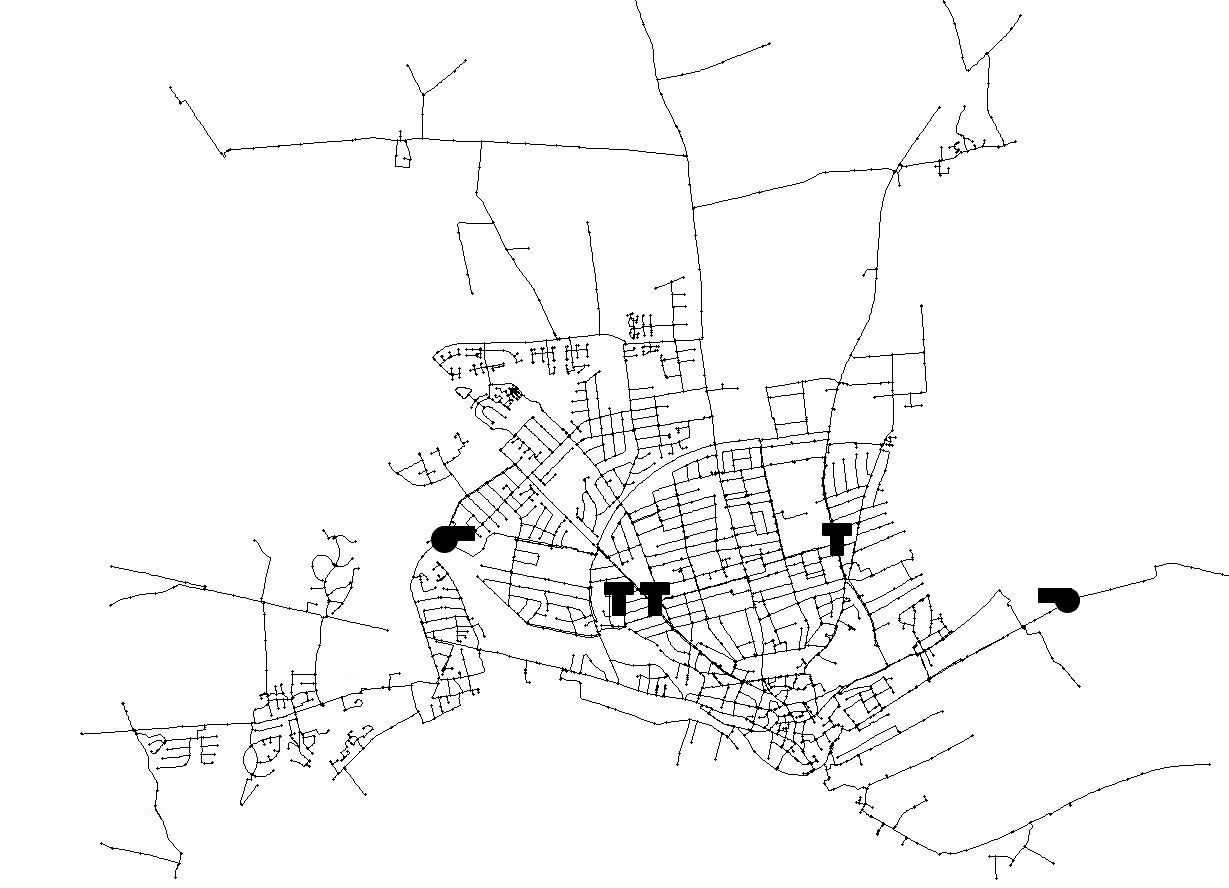
\includegraphics[width=\textwidth]{report/tikz/identification_map1}};
\node[black] at (11.4,4.75) {\footnotesize $\bm {\mathcal{W}_3}$};
\node[black] at (13.75,3.3) {\footnotesize $\bm {\mathcal{K}_2}$};
\node[black] at (4.7,4.65) {\footnotesize $\bm {\mathcal{K}_1}$};
\node[black] at (8.4,1) {\footnotesize $\bm {\mathcal{W}_2}$};
\node[black] at (6.8,1) {\footnotesize $\bm {\mathcal{W}_1}$};
\draw [-latex][thick](8.05,3.2) -- (8.4,1.35);
\draw [-latex][thick](7.55,3.2) -- (6.8,1.35);
\end{tikzpicture}

%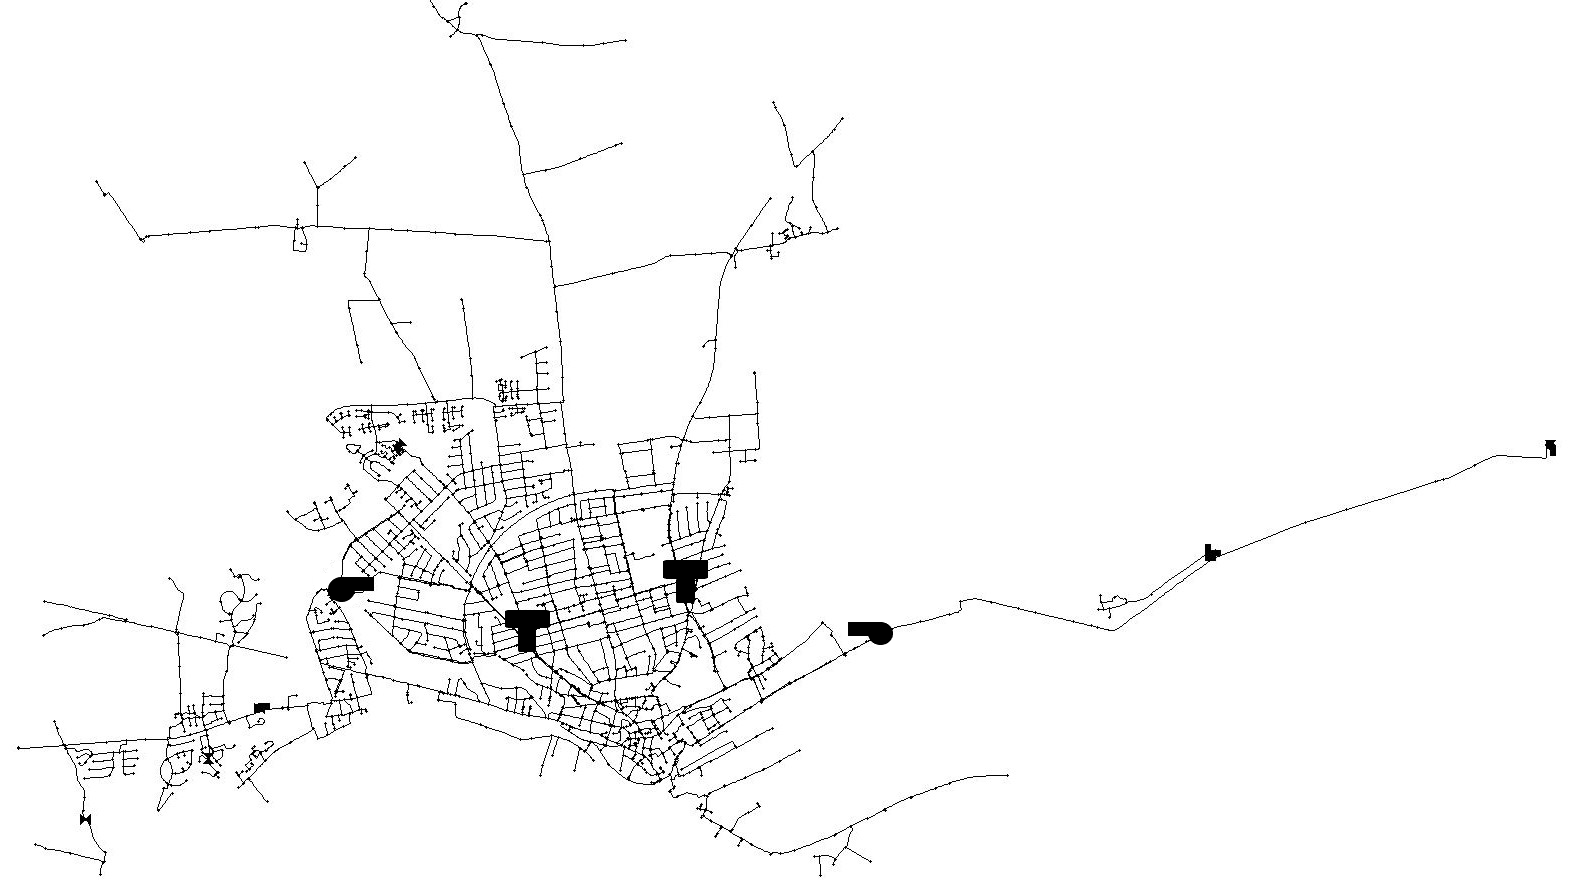
\includegraphics[width=0.95\textwidth]{report/pictures/verdo_pic3}
\caption{The network map with the corresponding WTs and pumping stations.}
\label{fig:simplified_network_identification1223}
\end{figure}
\vspace{-3mm}

In the following description, let us use the notation for the pumping stations and WTs shown in \figref{fig:simplified_network_identification1223}. Thus, $\mathcal{K}_1$ denotes Oust Mølle(OMV) waterwork and $\mathcal{K}_1$ denotes Toldbodgade(TBP) pumping station. The WTs at Hobrovej(HBP) pumping station are denoted with $\mathcal{W}_1$ and $\mathcal{W}_2$, furthermore the WT at Hadsundevej(HSP) pumping station is denoted with $\mathcal{W}_3$. 

The identification of the model has been carried out on measurement data provided by Verdo A/S, such that four days-long data sets have been extracted from three different time periods in 2017. It turned out to be difficult to find four day-long measurement sets, as certain sensors are frequently losing the radio signal, thus making the measurements unusable. The three data sets on which the identification and validations have been carried out is shown in \tabref{identification_periods}.

\begin{center}
    \begin{tabular}{ | p{3cm} | p{3cm} | p{3cm} |}
    \hline
     & \textbf{Start time} & \textbf{End time} \\ 
    \hline
    Period 1 & 21.10.2017 0.00 &  24.10.2017 23.00 \\ 
    \hline
    Period 2 & 07.11.2017 0.00 & 10.11.2017 23.00  \\ 
    \hline
    Period 3 & 09.12.2017 0.00 & 12.12.2017 23.00 \\ 
    \hline
    \end{tabular}
    \label{identification_periods}
    \captionof{table}{Dates from which data are extracted.}
\end{center}

\vspace{-3mm}

The model is first identified on the data set from Period 1. After the identification, the model is validated on the data sets from Period 2 and Period 3. The extracted data is sampled with $T_s = 1$ [min] sampling time, except for the total consumption $\sigma$, as it has been calculated by using the measurements on the WT flows. The sampling rate of the total water consumption $\sigma$ is $T_s = 1$ [h]. 

The total water consumption in the three different periods is shown in \figref{fig:data_allconsumption}, where $\sigma_1$, $\sigma_2$ and $\sigma_3$ denote the consumption in period 1, period 2 and period 3, respectively.

%Total consumptions
  \begin{figure}[H]
  \centering
  %\hspace{0mm}
  %
\includegraphics[width=0.35\textwidth]{report/pictures/missingfigure}
  % This file was created by matlab2tikz.
%
%The latest updates can be retrieved from
%  http://www.mathworks.com/matlabcentral/fileexchange/22022-matlab2tikz-matlab2tikz
%where you can also make suggestions and rate matlab2tikz.
%
\definecolor{mycolor1}{rgb}{0.00000,0.44700,0.74100}%
\definecolor{mycolor2}{rgb}{0.85000,0.32500,0.09800}%
\definecolor{mycolor3}{rgb}{0.92900,0.69400,0.12500}%
%
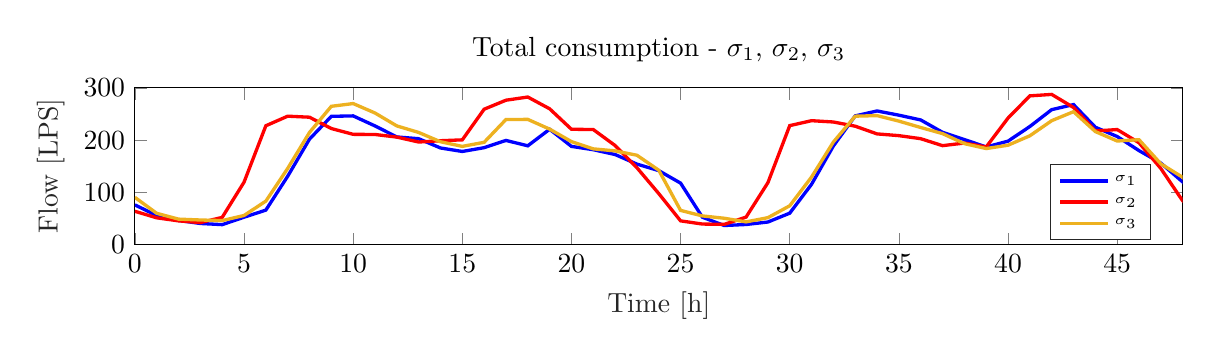
\begin{tikzpicture}

\begin{axis}[%
width=5.239in,
height=0.784in,
at={(1.013in,0.427in)},
scale only axis,
xmin=0,
xmax=48,
xlabel style={font=\color{white!15!black}},
xlabel={Time [h]},
ymin=0,
ymax=300,
ylabel style={font=\color{white!15!black}},
ylabel={Flow  [LPS]},
axis background/.style={fill=white},
title style={},
title={Total consumption - $\sigma_1$, $\sigma_2$, $\sigma_3$},
legend style={at={(0.97,0.03)}, anchor=south east, legend cell align=left, align=left, draw=white!15!black}
]
\addplot [color=blue, line width=1.2pt]
  table[row sep=crcr]{%
0	76.111111172\\
1	55.833333378\\
2	46.388888926\\
3	40.555555588\\
4	38.333333364\\
5	52.500000042\\
6	66.111111164\\
7	130.833333438\\
8	201.944444606\\
9	245.555555752\\
10	246.388889086\\
11	227.222222404\\
12	206.111111276\\
13	202.77777794\\
14	185.000000148\\
15	178.333333476\\
16	185.555555704\\
17	199.444444604\\
18	189.166666818\\
19	220.83333351\\
20	188.055555706\\
21	181.666666812\\
22	172.500000138\\
23	154.16666679\\
24	141.66666678\\
25	117.777777872\\
26	52.500000042\\
27	36.666666696\\
28	38.611111142\\
29	43.333333368\\
30	60.277777826\\
31	115.555555648\\
32	188.88888904\\
33	246.388889086\\
34	255.833333538\\
35	247.777777976\\
36	238.611111302\\
37	215.000000172\\
38	201.111111272\\
39	186.944444594\\
40	198.055555714\\
41	226.111111292\\
42	258.33333354\\
43	268.05555577\\
44	224.722222402\\
45	206.94444461\\
46	180.000000144\\
47	156.111111236\\
48	120.000000096\\
49	73.61111117\\
50	39.722222254\\
51	39.722222254\\
52	45.277777814\\
53	112.777777868\\
54	219.722222398\\
55	225.00000018\\
56	218.888889064\\
57	223.055555734\\
58	208.3333335\\
59	214.444444616\\
60	195.000000156\\
61	201.38888905\\
62	189.166666818\\
63	184.444444592\\
64	221.944444622\\
65	279.16666689\\
66	291.111111344\\
67	262.777777988\\
68	220.555555732\\
69	218.611111286\\
70	200.555555716\\
71	154.444444568\\
72	81.94444451\\
73	49.722222262\\
74	40.27777781\\
75	40.000000032\\
76	48.333333372\\
77	110.833333422\\
78	216.111111284\\
79	213.333333504\\
80	206.94444461\\
81	209.444444612\\
82	201.666666828\\
83	202.77777794\\
84	191.944444598\\
85	189.444444596\\
86	183.888889036\\
87	209.166666834\\
88	252.222222424\\
89	271.388889106\\
90	279.16666689\\
91	253.055555758\\
92	217.777777952\\
93	210.000000168\\
94	186.388889038\\
95	146.111111228\\
};
\addlegendentry{\tiny $\sigma_1$}

\addplot [color=red, line width=1.2pt]
  table[row sep=crcr]{%
0	63.88888894\\
1	51.38888893\\
2	45.555555592\\
3	42.222222256\\
4	52.222222264\\
5	119.44444454\\
6	227.500000182\\
7	245.83333353\\
8	243.888889084\\
9	222.2222224\\
10	211.11111128\\
11	210.833333502\\
12	205.833333498\\
13	196.388889046\\
14	198.888889048\\
15	200.555555716\\
16	259.166666874\\
17	276.38888911\\
18	282.500000226\\
19	260.000000208\\
20	220.83333351\\
21	220.277777954\\
22	189.722222374\\
23	147.22222234\\
24	97.777777856\\
25	45.555555592\\
26	39.444444476\\
27	38.88888892\\
28	52.77777782\\
29	118.611111206\\
30	227.77777796\\
31	237.222222412\\
32	234.72222241\\
33	226.666666848\\
34	211.944444614\\
35	208.611111278\\
36	202.77777794\\
37	189.444444596\\
38	194.4444446\\
39	186.944444594\\
40	242.222222416\\
41	284.72222245\\
42	287.50000023\\
43	262.50000021\\
44	217.500000174\\
45	220.277777954\\
46	195.000000156\\
47	145.83333345\\
48	83.888888956\\
49	47.22222226\\
50	46.388888926\\
51	42.777777812\\
52	51.666666708\\
53	118.888888984\\
54	231.388889074\\
55	236.666666856\\
56	216.66666684\\
57	226.666666848\\
58	213.055555726\\
59	209.166666834\\
60	202.222222384\\
61	193.888889044\\
62	189.722222374\\
63	198.888889048\\
64	262.50000021\\
65	286.11111134\\
66	282.222222448\\
67	265.555555768\\
68	220.000000176\\
69	216.388889062\\
70	193.888889044\\
71	153.333333456\\
72	99.166666746\\
73	50.833333374\\
74	46.111111148\\
75	47.500000038\\
76	56.94444449\\
77	120.000000096\\
78	223.61111129\\
79	240.000000192\\
80	223.333333512\\
81	235.555555744\\
82	210.000000168\\
83	216.388889062\\
84	203.333333496\\
85	214.444444616\\
86	206.388889054\\
87	224.444444624\\
88	271.388889106\\
89	267.777777992\\
90	259.166666874\\
91	236.666666856\\
92	201.666666828\\
93	199.722222382\\
94	187.777777928\\
95	130.833333438\\
};
\addlegendentry{\tiny $\sigma_2$}

\addplot [color=mycolor3, line width=1.2pt]
  table[row sep=crcr]{%
0	90.555555628\\
1	60.000000048\\
2	48.888888928\\
3	47.22222226\\
4	46.111111148\\
5	55.833333378\\
6	83.3333334\\
7	145.83333345\\
8	214.722222394\\
9	264.722222434\\
10	270.000000216\\
11	251.944444646\\
12	227.222222404\\
13	214.722222394\\
14	196.944444602\\
15	188.055555706\\
16	195.83333349\\
17	239.444444636\\
18	239.722222414\\
19	221.111111288\\
20	197.22222238\\
21	183.33333348\\
22	179.444444588\\
23	171.111111248\\
24	142.500000114\\
25	65.555555608\\
26	55.000000044\\
27	50.555555596\\
28	43.611111146\\
29	51.666666708\\
30	74.444444504\\
31	129.444444548\\
32	196.388889046\\
33	245.83333353\\
34	246.944444642\\
35	236.388889078\\
36	224.166666846\\
37	212.50000017\\
38	193.333333488\\
39	183.888889036\\
40	190.27777793\\
41	208.3333335\\
42	237.222222412\\
43	254.444444648\\
44	216.388889062\\
45	198.333333492\\
46	200.833333494\\
47	154.722222346\\
48	128.888888992\\
49	81.94444451\\
50	40.27777781\\
51	39.166666698\\
52	50.555555596\\
53	123.61111121\\
54	225.555555736\\
55	235.833333522\\
56	221.944444622\\
57	227.500000182\\
58	221.388889066\\
59	225.833333514\\
60	211.11111128\\
61	202.222222384\\
62	188.88888904\\
63	195.83333349\\
64	239.166666858\\
65	281.111111336\\
66	290.555555788\\
67	263.055555766\\
68	227.500000182\\
69	220.555555732\\
70	205.833333498\\
71	150.555555676\\
72	75.00000006\\
73	53.333333376\\
74	43.05555559\\
75	44.166666702\\
76	60.000000048\\
77	121.111111208\\
78	221.111111288\\
79	229.444444628\\
80	212.777777948\\
81	218.888889064\\
82	211.944444614\\
83	205.000000164\\
84	195.555555712\\
85	198.888889048\\
86	189.444444596\\
87	221.111111288\\
88	258.888889096\\
89	263.055555766\\
90	269.166666882\\
91	262.777777988\\
92	220.555555732\\
93	210.000000168\\
94	192.222222376\\
95	155.000000124\\
};
\addlegendentry{\tiny $\sigma_3$}

\end{axis}
\end{tikzpicture}% 
  %\vspace{-2.5mm}
  \caption{Total water consumption in three different periods.}
  \label{fig:data_allconsumption}
  \end{figure}
 %\vspace{-8mm}

As it is shown in \figref{fig:data_allconsumption}, the characteristics of the daily consumption is similar, although measurements are taken from different months. 

%Inlet flows - period 1
  \begin{figure}[H]
  \centering
  %\hspace{0mm}
  %
\includegraphics[width=0.35\textwidth]{report/pictures/missingfigure}
  % This file was created by matlab2tikz.
%
%The latest updates can be retrieved from
%  http://www.mathworks.com/matlabcentral/fileexchange/22022-matlab2tikz-matlab2tikz
%where you can also make suggestions and rate matlab2tikz.
%
\definecolor{mycolor1}{rgb}{0.00000,0.44700,0.74100}%
\definecolor{mycolor2}{rgb}{0.85000,0.32500,0.09800}%
%
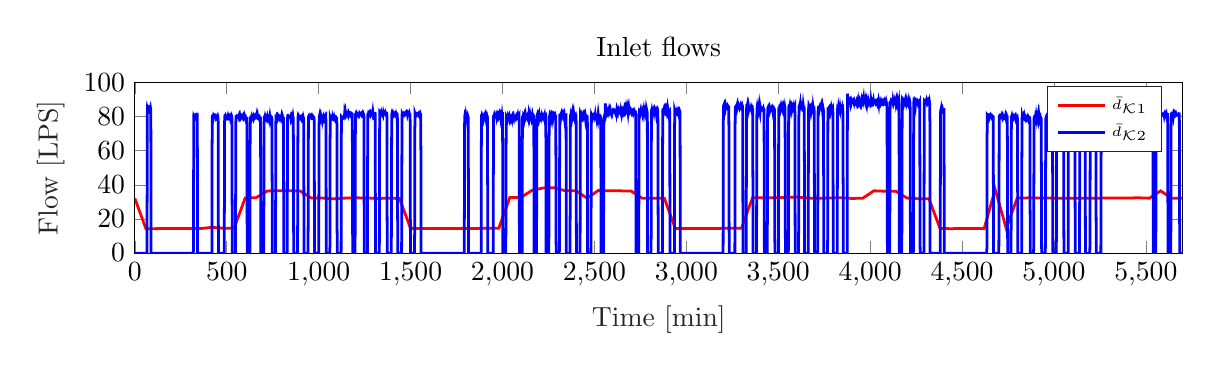
\begin{tikzpicture}

\begin{axis}[%
width=5.239in,
height=0.854in,
at={(1.02in,0.431in)},
scale only axis,
xmin=0,
xmax=5700,
xlabel style={font=\color{white!15!black}},
xlabel={Time [min]},
ymin=-0.1944444446,
ymax=100,
ylabel style={font=\color{white!15!black}},
ylabel={Flow  [LPS]},
axis background/.style={fill=white},
title style={},
title={Inlet flows},
legend style={legend cell align=left, align=left, draw=white!15!black}
]
\addplot [color=red, line width=1.0pt, forget plot]
  table[row sep=crcr]{%
0	32.0000000256\\
1	31.70416669203\\
2	31.40833335846\\
3	31.11250002489\\
4	30.81666669132\\
5	30.52083335775\\
6	30.22500002418\\
7	29.92916669061\\
8	29.63333335704\\
9	29.33750002347\\
10	29.0416666899\\
11	28.74583335633\\
12	28.45000002276\\
13	28.15416668919\\
14	27.85833335562\\
15	27.56250002205\\
16	27.26666668848\\
17	26.97083335491\\
18	26.67500002134\\
19	26.37916668777\\
20	26.0833333542\\
21	25.78750002063\\
22	25.49166668706\\
23	25.19583335349\\
24	24.90000001992\\
25	24.60416668635\\
26	24.30833335278\\
27	24.01250001921\\
28	23.71666668564\\
29	23.42083335207\\
30	23.1250000185\\
31	22.82916668493\\
32	22.53333335136\\
33	22.23750001779\\
34	21.94166668422\\
35	21.64583335065\\
36	21.35000001708\\
37	21.05416668351\\
38	20.75833334994\\
39	20.46250001637\\
40	20.1666666828\\
41	19.87083334923\\
42	19.57500001566\\
43	19.27916668209\\
44	18.98333334852\\
45	18.68750001495\\
46	18.39166668138\\
47	18.09583334781\\
48	17.80000001424\\
49	17.50416668067\\
50	17.2083333471\\
51	16.91250001353\\
52	16.61666667996\\
53	16.32083334639\\
54	16.02500001282\\
55	15.72916667925\\
56	15.43333334568\\
57	15.13750001211\\
58	14.84166667854\\
59	14.54583334497\\
60	14.2500000114\\
61	14.2504629743633\\
62	14.2509259373267\\
63	14.25138890029\\
64	14.2518518632533\\
65	14.2523148262167\\
66	14.25277778918\\
67	14.2532407521433\\
68	14.2537037151067\\
69	14.25416667807\\
70	14.2546296410333\\
71	14.2550926039967\\
72	14.25555556696\\
73	14.2560185299233\\
74	14.2564814928867\\
75	14.25694445585\\
76	14.2574074188133\\
77	14.2578703817767\\
78	14.25833334474\\
79	14.2587963077033\\
80	14.2592592706667\\
81	14.25972223363\\
82	14.2601851965933\\
83	14.2606481595567\\
84	14.26111112252\\
85	14.2615740854833\\
86	14.2620370484467\\
87	14.26250001141\\
88	14.2629629743733\\
89	14.2634259373367\\
90	14.2638889003\\
91	14.2643518632633\\
92	14.2648148262267\\
93	14.26527778919\\
94	14.2657407521533\\
95	14.2662037151167\\
96	14.26666667808\\
97	14.2671296410433\\
98	14.2675926040067\\
99	14.26805556697\\
100	14.2685185299333\\
101	14.2689814928967\\
102	14.26944445586\\
103	14.2699074188233\\
104	14.2703703817867\\
105	14.27083334475\\
106	14.2712963077133\\
107	14.2717592706767\\
108	14.27222223364\\
109	14.2726851966033\\
110	14.2731481595667\\
111	14.27361112253\\
112	14.2740740854933\\
113	14.2745370484567\\
114	14.27500001142\\
115	14.2754629743833\\
116	14.2759259373467\\
117	14.27638890031\\
118	14.2768518632733\\
119	14.2773148262367\\
120	14.2777777892\\
121	14.2787037151267\\
122	14.2796296410533\\
123	14.28055556698\\
124	14.2814814929067\\
125	14.2824074188333\\
126	14.28333334476\\
127	14.2842592706867\\
128	14.2851851966133\\
129	14.28611112254\\
130	14.2870370484667\\
131	14.2879629743933\\
132	14.28888890032\\
133	14.2898148262467\\
134	14.2907407521733\\
135	14.2916666781\\
136	14.2925926040267\\
137	14.2935185299533\\
138	14.29444445588\\
139	14.2953703818067\\
140	14.2962963077333\\
141	14.29722223366\\
142	14.2981481595867\\
143	14.2990740855133\\
144	14.30000001144\\
145	14.3009259373667\\
146	14.3018518632933\\
147	14.30277778922\\
148	14.3037037151467\\
149	14.3046296410733\\
150	14.305555567\\
151	14.3064814929267\\
152	14.3074074188533\\
153	14.30833334478\\
154	14.3092592707067\\
155	14.3101851966333\\
156	14.31111112256\\
157	14.3120370484867\\
158	14.3129629744133\\
159	14.31388890034\\
160	14.3148148262667\\
161	14.3157407521933\\
162	14.31666667812\\
163	14.3175926040467\\
164	14.3185185299733\\
165	14.3194444559\\
166	14.3203703818267\\
167	14.3212963077533\\
168	14.32222223368\\
169	14.3231481596067\\
170	14.3240740855333\\
171	14.32500001146\\
172	14.3259259373867\\
173	14.3268518633133\\
174	14.32777778924\\
175	14.3287037151667\\
176	14.3296296410933\\
177	14.33055556702\\
178	14.3314814929467\\
179	14.3324074188733\\
180	14.3333333448\\
181	14.3333333448\\
182	14.3333333448\\
183	14.3333333448\\
184	14.3333333448\\
185	14.3333333448\\
186	14.3333333448\\
187	14.3333333448\\
188	14.3333333448\\
189	14.3333333448\\
190	14.3333333448\\
191	14.3333333448\\
192	14.3333333448\\
193	14.3333333448\\
194	14.3333333448\\
195	14.3333333448\\
196	14.3333333448\\
197	14.3333333448\\
198	14.3333333448\\
199	14.3333333448\\
200	14.3333333448\\
201	14.3333333448\\
202	14.3333333448\\
203	14.3333333448\\
204	14.3333333448\\
205	14.3333333448\\
206	14.3333333448\\
207	14.3333333448\\
208	14.3333333448\\
209	14.3333333448\\
210	14.3333333448\\
211	14.3333333448\\
212	14.3333333448\\
213	14.3333333448\\
214	14.3333333448\\
215	14.3333333448\\
216	14.3333333448\\
217	14.3333333448\\
218	14.3333333448\\
219	14.3333333448\\
220	14.3333333448\\
221	14.3333333448\\
222	14.3333333448\\
223	14.3333333448\\
224	14.3333333448\\
225	14.3333333448\\
226	14.3333333448\\
227	14.3333333448\\
228	14.3333333448\\
229	14.3333333448\\
230	14.3333333448\\
231	14.3333333448\\
232	14.3333333448\\
233	14.3333333448\\
234	14.3333333448\\
235	14.3333333448\\
236	14.3333333448\\
237	14.3333333448\\
238	14.3333333448\\
239	14.3333333448\\
240	14.3333333448\\
241	14.3324074188733\\
242	14.3314814929467\\
243	14.33055556702\\
244	14.3296296410933\\
245	14.3287037151667\\
246	14.32777778924\\
247	14.3268518633133\\
248	14.3259259373867\\
249	14.32500001146\\
250	14.3240740855333\\
251	14.3231481596067\\
252	14.32222223368\\
253	14.3212963077533\\
254	14.3203703818267\\
255	14.3194444559\\
256	14.3185185299733\\
257	14.3175926040467\\
258	14.31666667812\\
259	14.3157407521933\\
260	14.3148148262667\\
261	14.31388890034\\
262	14.3129629744133\\
263	14.3120370484867\\
264	14.31111112256\\
265	14.3101851966333\\
266	14.3092592707067\\
267	14.30833334478\\
268	14.3074074188533\\
269	14.3064814929267\\
270	14.305555567\\
271	14.3046296410733\\
272	14.3037037151467\\
273	14.30277778922\\
274	14.3018518632933\\
275	14.3009259373667\\
276	14.30000001144\\
277	14.2990740855133\\
278	14.2981481595867\\
279	14.29722223366\\
280	14.2962963077333\\
281	14.2953703818067\\
282	14.29444445588\\
283	14.2935185299533\\
284	14.2925926040267\\
285	14.2916666781\\
286	14.2907407521733\\
287	14.2898148262467\\
288	14.28888890032\\
289	14.2879629743933\\
290	14.2870370484667\\
291	14.28611112254\\
292	14.2851851966133\\
293	14.2842592706867\\
294	14.28333334476\\
295	14.2824074188333\\
296	14.2814814929067\\
297	14.28055556698\\
298	14.2796296410533\\
299	14.2787037151267\\
300	14.2777777892\\
301	14.27916667809\\
302	14.28055556698\\
303	14.28194445587\\
304	14.28333334476\\
305	14.28472223365\\
306	14.28611112254\\
307	14.28750001143\\
308	14.28888890032\\
309	14.29027778921\\
310	14.2916666781\\
311	14.29305556699\\
312	14.29444445588\\
313	14.29583334477\\
314	14.29722223366\\
315	14.29861112255\\
316	14.30000001144\\
317	14.30138890033\\
318	14.30277778922\\
319	14.30416667811\\
320	14.305555567\\
321	14.30694445589\\
322	14.30833334478\\
323	14.30972223367\\
324	14.31111112256\\
325	14.31250001145\\
326	14.31388890034\\
327	14.31527778923\\
328	14.31666667812\\
329	14.31805556701\\
330	14.3194444559\\
331	14.32083334479\\
332	14.32222223368\\
333	14.32361112257\\
334	14.32500001146\\
335	14.32638890035\\
336	14.32777778924\\
337	14.32916667813\\
338	14.33055556702\\
339	14.33194445591\\
340	14.3333333448\\
341	14.33472223369\\
342	14.33611112258\\
343	14.33750001147\\
344	14.33888890036\\
345	14.34027778925\\
346	14.34166667814\\
347	14.34305556703\\
348	14.34444445592\\
349	14.34583334481\\
350	14.3472222337\\
351	14.34861112259\\
352	14.35000001148\\
353	14.35138890037\\
354	14.35277778926\\
355	14.35416667815\\
356	14.35555556704\\
357	14.35694445593\\
358	14.35833334482\\
359	14.35972223371\\
360	14.3611111226\\
361	14.37222223372\\
362	14.38333334484\\
363	14.39444445596\\
364	14.40555556708\\
365	14.4166666782\\
366	14.42777778932\\
367	14.43888890044\\
368	14.45000001156\\
369	14.46111112268\\
370	14.4722222338\\
371	14.48333334492\\
372	14.49444445604\\
373	14.50555556716\\
374	14.51666667828\\
375	14.5277777894\\
376	14.53888890052\\
377	14.55000001164\\
378	14.56111112276\\
379	14.57222223388\\
380	14.583333345\\
381	14.59444445612\\
382	14.60555556724\\
383	14.61666667836\\
384	14.62777778948\\
385	14.6388889006\\
386	14.65000001172\\
387	14.66111112284\\
388	14.67222223396\\
389	14.68333334508\\
390	14.6944444562\\
391	14.70555556732\\
392	14.71666667844\\
393	14.72777778956\\
394	14.73888890068\\
395	14.7500000118\\
396	14.76111112292\\
397	14.77222223404\\
398	14.78333334516\\
399	14.79444445628\\
400	14.8055555674\\
401	14.81666667852\\
402	14.82777778964\\
403	14.83888890076\\
404	14.85000001188\\
405	14.861111123\\
406	14.87222223412\\
407	14.88333334524\\
408	14.89444445636\\
409	14.90555556748\\
410	14.9166666786\\
411	14.92777778972\\
412	14.93888890084\\
413	14.95000001196\\
414	14.96111112308\\
415	14.9722222342\\
416	14.98333334532\\
417	14.99444445644\\
418	15.00555556756\\
419	15.01666667868\\
420	15.0277777898\\
421	15.01944445646\\
422	15.01111112312\\
423	15.00277778978\\
424	14.99444445644\\
425	14.9861111231\\
426	14.97777778976\\
427	14.96944445642\\
428	14.96111112308\\
429	14.95277778974\\
430	14.9444444564\\
431	14.93611112306\\
432	14.92777778972\\
433	14.91944445638\\
434	14.91111112304\\
435	14.9027777897\\
436	14.89444445636\\
437	14.88611112302\\
438	14.87777778968\\
439	14.86944445634\\
440	14.861111123\\
441	14.85277778966\\
442	14.84444445632\\
443	14.83611112298\\
444	14.82777778964\\
445	14.8194444563\\
446	14.81111112296\\
447	14.80277778962\\
448	14.79444445628\\
449	14.78611112294\\
450	14.7777777896\\
451	14.76944445626\\
452	14.76111112292\\
453	14.75277778958\\
454	14.74444445624\\
455	14.7361111229\\
456	14.72777778956\\
457	14.71944445622\\
458	14.71111112288\\
459	14.70277778954\\
460	14.6944444562\\
461	14.68611112286\\
462	14.67777778952\\
463	14.66944445618\\
464	14.66111112284\\
465	14.6527777895\\
466	14.64444445616\\
467	14.63611112282\\
468	14.62777778948\\
469	14.61944445614\\
470	14.6111111228\\
471	14.60277778946\\
472	14.59444445612\\
473	14.58611112278\\
474	14.57777778944\\
475	14.5694444561\\
476	14.56111112276\\
477	14.55277778942\\
478	14.54444445608\\
479	14.53611112274\\
480	14.5277777894\\
481	14.5277777894\\
482	14.5277777894\\
483	14.5277777894\\
484	14.5277777894\\
485	14.5277777894\\
486	14.5277777894\\
487	14.5277777894\\
488	14.5277777894\\
489	14.5277777894\\
490	14.5277777894\\
491	14.5277777894\\
492	14.5277777894\\
493	14.5277777894\\
494	14.5277777894\\
495	14.5277777894\\
496	14.5277777894\\
497	14.5277777894\\
498	14.5277777894\\
499	14.5277777894\\
500	14.5277777894\\
501	14.5277777894\\
502	14.5277777894\\
503	14.5277777894\\
504	14.5277777894\\
505	14.5277777894\\
506	14.5277777894\\
507	14.5277777894\\
508	14.5277777894\\
509	14.5277777894\\
510	14.5277777894\\
511	14.5277777894\\
512	14.5277777894\\
513	14.5277777894\\
514	14.5277777894\\
515	14.5277777894\\
516	14.5277777894\\
517	14.5277777894\\
518	14.5277777894\\
519	14.5277777894\\
520	14.5277777894\\
521	14.5277777894\\
522	14.5277777894\\
523	14.5277777894\\
524	14.5277777894\\
525	14.5277777894\\
526	14.5277777894\\
527	14.5277777894\\
528	14.5277777894\\
529	14.5277777894\\
530	14.5277777894\\
531	14.5277777894\\
532	14.5277777894\\
533	14.5277777894\\
534	14.5277777894\\
535	14.5277777894\\
536	14.5277777894\\
537	14.5277777894\\
538	14.5277777894\\
539	14.5277777894\\
540	14.5277777894\\
541	14.8231481600066\\
542	15.1185185306133\\
543	15.41388890122\\
544	15.7092592718267\\
545	16.0046296424333\\
546	16.30000001304\\
547	16.5953703836467\\
548	16.8907407542533\\
549	17.18611112486\\
550	17.4814814954667\\
551	17.7768518660733\\
552	18.07222223668\\
553	18.3675926072867\\
554	18.6629629778933\\
555	18.9583333485\\
556	19.2537037191066\\
557	19.5490740897133\\
558	19.84444446032\\
559	20.1398148309267\\
560	20.4351852015333\\
561	20.73055557214\\
562	21.0259259427467\\
563	21.3212963133533\\
564	21.61666668396\\
565	21.9120370545667\\
566	22.2074074251733\\
567	22.50277779578\\
568	22.7981481663867\\
569	23.0935185369933\\
570	23.3888889076\\
571	23.6842592782066\\
572	23.9796296488133\\
573	24.27500001942\\
574	24.5703703900267\\
575	24.8657407606333\\
576	25.16111113124\\
577	25.4564815018467\\
578	25.7518518724533\\
579	26.04722224306\\
580	26.3425926136667\\
581	26.6379629842733\\
582	26.93333335488\\
583	27.2287037254867\\
584	27.5240740960933\\
585	27.8194444667\\
586	28.1148148373067\\
587	28.4101852079133\\
588	28.70555557852\\
589	29.0009259491267\\
590	29.2962963197333\\
591	29.59166669034\\
592	29.8870370609467\\
593	30.1824074315533\\
594	30.47777780216\\
595	30.7731481727667\\
596	31.0685185433733\\
597	31.36388891398\\
598	31.6592592845867\\
599	31.9546296551933\\
600	32.2500000258\\
601	32.2532407665433\\
602	32.2564815072867\\
603	32.25972224803\\
604	32.2629629887733\\
605	32.2662037295167\\
606	32.26944447026\\
607	32.2726852110033\\
608	32.2759259517467\\
609	32.27916669249\\
610	32.2824074332333\\
611	32.2856481739767\\
612	32.28888891472\\
613	32.2921296554633\\
614	32.2953703962067\\
615	32.29861113695\\
616	32.3018518776933\\
617	32.3050926184367\\
618	32.30833335918\\
619	32.3115740999233\\
620	32.3148148406667\\
621	32.31805558141\\
622	32.3212963221533\\
623	32.3245370628967\\
624	32.32777780364\\
625	32.3310185443833\\
626	32.3342592851267\\
627	32.33750002587\\
628	32.3407407666133\\
629	32.3439815073567\\
630	32.3472222481\\
631	32.3504629888433\\
632	32.3537037295867\\
633	32.35694447033\\
634	32.3601852110733\\
635	32.3634259518167\\
636	32.36666669256\\
637	32.3699074333033\\
638	32.3731481740467\\
639	32.37638891479\\
640	32.3796296555333\\
641	32.3828703962767\\
642	32.38611113702\\
643	32.3893518777633\\
644	32.3925926185067\\
645	32.39583335925\\
646	32.3990740999933\\
647	32.4023148407367\\
648	32.40555558148\\
649	32.4087963222233\\
650	32.4120370629667\\
651	32.41527780371\\
652	32.4185185444533\\
653	32.4217592851967\\
654	32.42500002594\\
655	32.4282407666833\\
656	32.4314815074267\\
657	32.43472224817\\
658	32.4379629889133\\
659	32.4412037296567\\
660	32.4444444704\\
661	32.5101852111933\\
662	32.5759259519867\\
663	32.64166669278\\
664	32.7074074335733\\
665	32.7731481743667\\
666	32.83888891516\\
667	32.9046296559533\\
668	32.9703703967467\\
669	33.03611113754\\
670	33.1018518783333\\
671	33.1675926191267\\
672	33.23333335992\\
673	33.2990741007133\\
674	33.3648148415067\\
675	33.4305555823\\
676	33.4962963230933\\
677	33.5620370638867\\
678	33.62777780468\\
679	33.6935185454733\\
680	33.7592592862667\\
681	33.82500002706\\
682	33.8907407678533\\
683	33.9564815086467\\
684	34.02222224944\\
685	34.0879629902333\\
686	34.1537037310267\\
687	34.21944447182\\
688	34.2851852126133\\
689	34.3509259534067\\
690	34.4166666942\\
691	34.4824074349933\\
692	34.5481481757867\\
693	34.61388891658\\
694	34.6796296573733\\
695	34.7453703981667\\
696	34.81111113896\\
697	34.8768518797533\\
698	34.9425926205467\\
699	35.00833336134\\
700	35.0740741021333\\
701	35.1398148429267\\
702	35.20555558372\\
703	35.2712963245133\\
704	35.3370370653067\\
705	35.4027778061\\
706	35.4685185468933\\
707	35.5342592876867\\
708	35.60000002848\\
709	35.6657407692733\\
710	35.7314815100667\\
711	35.79722225086\\
712	35.8629629916533\\
713	35.9287037324467\\
714	35.99444447324\\
715	36.0601852140333\\
716	36.1259259548267\\
717	36.19166669562\\
718	36.2574074364133\\
719	36.3231481772067\\
720	36.388888918\\
721	36.3912037328167\\
722	36.3935185476333\\
723	36.39583336245\\
724	36.3981481772667\\
725	36.4004629920833\\
726	36.4027778069\\
727	36.4050926217167\\
728	36.4074074365333\\
729	36.40972225135\\
730	36.4120370661667\\
731	36.4143518809833\\
732	36.4166666958\\
733	36.4189815106167\\
734	36.4212963254333\\
735	36.42361114025\\
736	36.4259259550667\\
737	36.4282407698833\\
738	36.4305555847\\
739	36.4328703995167\\
740	36.4351852143333\\
741	36.43750002915\\
742	36.4398148439667\\
743	36.4421296587833\\
744	36.4444444736\\
745	36.4467592884167\\
746	36.4490741032333\\
747	36.45138891805\\
748	36.4537037328667\\
749	36.4560185476833\\
750	36.4583333625\\
751	36.4606481773167\\
752	36.4629629921333\\
753	36.46527780695\\
754	36.4675926217667\\
755	36.4699074365833\\
756	36.4722222514\\
757	36.4745370662167\\
758	36.4768518810333\\
759	36.47916669585\\
760	36.4814815106667\\
761	36.4837963254833\\
762	36.4861111403\\
763	36.4884259551167\\
764	36.4907407699333\\
765	36.49305558475\\
766	36.4953703995667\\
767	36.4976852143833\\
768	36.5000000292\\
769	36.5023148440167\\
770	36.5046296588333\\
771	36.50694447365\\
772	36.5092592884667\\
773	36.5115741032833\\
774	36.5138889181\\
775	36.5162037329167\\
776	36.5185185477333\\
777	36.52083336255\\
778	36.5231481773667\\
779	36.5254629921833\\
780	36.527777807\\
781	36.5273148440367\\
782	36.5268518810733\\
783	36.52638891811\\
784	36.5259259551467\\
785	36.5254629921833\\
786	36.52500002922\\
787	36.5245370662567\\
788	36.5240741032933\\
789	36.52361114033\\
790	36.5231481773667\\
791	36.5226852144033\\
792	36.52222225144\\
793	36.5217592884767\\
794	36.5212963255133\\
795	36.52083336255\\
796	36.5203703995867\\
797	36.5199074366233\\
798	36.51944447366\\
799	36.5189815106967\\
800	36.5185185477333\\
801	36.51805558477\\
802	36.5175926218067\\
803	36.5171296588433\\
804	36.51666669588\\
805	36.5162037329167\\
806	36.5157407699533\\
807	36.51527780699\\
808	36.5148148440267\\
809	36.5143518810633\\
810	36.5138889181\\
811	36.5134259551367\\
812	36.5129629921733\\
813	36.51250002921\\
814	36.5120370662467\\
815	36.5115741032833\\
816	36.51111114032\\
817	36.5106481773567\\
818	36.5101852143933\\
819	36.50972225143\\
820	36.5092592884667\\
821	36.5087963255033\\
822	36.50833336254\\
823	36.5078703995767\\
824	36.5074074366133\\
825	36.50694447365\\
826	36.5064815106867\\
827	36.5060185477233\\
828	36.50555558476\\
829	36.5050926217967\\
830	36.5046296588333\\
831	36.50416669587\\
832	36.5037037329067\\
833	36.5032407699433\\
834	36.50277780698\\
835	36.5023148440167\\
836	36.5018518810533\\
837	36.50138891809\\
838	36.5009259551267\\
839	36.5004629921633\\
840	36.5000000292\\
841	36.49722225142\\
842	36.49444447364\\
843	36.49166669586\\
844	36.48888891808\\
845	36.4861111403\\
846	36.48333336252\\
847	36.48055558474\\
848	36.47777780696\\
849	36.47500002918\\
850	36.4722222514\\
851	36.46944447362\\
852	36.46666669584\\
853	36.46388891806\\
854	36.46111114028\\
855	36.4583333625\\
856	36.45555558472\\
857	36.45277780694\\
858	36.45000002916\\
859	36.44722225138\\
860	36.4444444736\\
861	36.44166669582\\
862	36.43888891804\\
863	36.43611114026\\
864	36.43333336248\\
865	36.4305555847\\
866	36.42777780692\\
867	36.42500002914\\
868	36.42222225136\\
869	36.41944447358\\
870	36.4166666958\\
871	36.41388891802\\
872	36.41111114024\\
873	36.40833336246\\
874	36.40555558468\\
875	36.4027778069\\
876	36.40000002912\\
877	36.39722225134\\
878	36.39444447356\\
879	36.39166669578\\
880	36.388888918\\
881	36.38611114022\\
882	36.38333336244\\
883	36.38055558466\\
884	36.37777780688\\
885	36.3750000291\\
886	36.37222225132\\
887	36.36944447354\\
888	36.36666669576\\
889	36.36388891798\\
890	36.3611111402\\
891	36.35833336242\\
892	36.35555558464\\
893	36.35277780686\\
894	36.35000002908\\
895	36.3472222513\\
896	36.34444447352\\
897	36.34166669574\\
898	36.33888891796\\
899	36.33611114018\\
900	36.3333333624\\
901	36.2648148438267\\
902	36.1962963252533\\
903	36.12777780668\\
904	36.0592592881067\\
905	35.9907407695333\\
906	35.92222225096\\
907	35.8537037323867\\
908	35.7851852138133\\
909	35.71666669524\\
910	35.6481481766667\\
911	35.5796296580933\\
912	35.51111113952\\
913	35.4425926209467\\
914	35.3740741023733\\
915	35.3055555838\\
916	35.2370370652267\\
917	35.1685185466533\\
918	35.10000002808\\
919	35.0314815095067\\
920	34.9629629909333\\
921	34.89444447236\\
922	34.8259259537867\\
923	34.7574074352133\\
924	34.68888891664\\
925	34.6203703980667\\
926	34.5518518794933\\
927	34.48333336092\\
928	34.4148148423467\\
929	34.3462963237733\\
930	34.2777778052\\
931	34.2092592866267\\
932	34.1407407680533\\
933	34.07222224948\\
934	34.0037037309067\\
935	33.9351852123333\\
936	33.86666669376\\
937	33.7981481751867\\
938	33.7296296566133\\
939	33.66111113804\\
940	33.5925926194667\\
941	33.5240741008933\\
942	33.45555558232\\
943	33.3870370637467\\
944	33.3185185451733\\
945	33.2500000266\\
946	33.1814815080267\\
947	33.1129629894533\\
948	33.04444447088\\
949	32.9759259523067\\
950	32.9074074337333\\
951	32.83888891516\\
952	32.7703703965867\\
953	32.7018518780133\\
954	32.63333335944\\
955	32.5648148408667\\
956	32.4962963222933\\
957	32.42777780372\\
958	32.3592592851467\\
959	32.2907407665733\\
960	32.222222248\\
961	32.2217592850367\\
962	32.2212963220733\\
963	32.22083335911\\
964	32.2203703961467\\
965	32.2199074331833\\
966	32.21944447022\\
967	32.2189815072567\\
968	32.2185185442933\\
969	32.21805558133\\
970	32.2175926183667\\
971	32.2171296554033\\
972	32.21666669244\\
973	32.2162037294767\\
974	32.2157407665133\\
975	32.21527780355\\
976	32.2148148405867\\
977	32.2143518776233\\
978	32.21388891466\\
979	32.2134259516967\\
980	32.2129629887333\\
981	32.21250002577\\
982	32.2120370628067\\
983	32.2115740998433\\
984	32.21111113688\\
985	32.2106481739167\\
986	32.2101852109533\\
987	32.20972224799\\
988	32.2092592850267\\
989	32.2087963220633\\
990	32.2083333591\\
991	32.2078703961367\\
992	32.2074074331733\\
993	32.20694447021\\
994	32.2064815072467\\
995	32.2060185442833\\
996	32.20555558132\\
997	32.2050926183567\\
998	32.2046296553933\\
999	32.20416669243\\
1000	32.2037037294667\\
1001	32.2032407665033\\
1002	32.20277780354\\
1003	32.2023148405767\\
1004	32.2018518776133\\
1005	32.20138891465\\
1006	32.2009259516867\\
1007	32.2004629887233\\
1008	32.20000002576\\
1009	32.1995370627967\\
1010	32.1990740998333\\
1011	32.19861113687\\
1012	32.1981481739067\\
1013	32.1976852109433\\
1014	32.19722224798\\
1015	32.1967592850167\\
1016	32.1962963220533\\
1017	32.19583335909\\
1018	32.1953703961267\\
1019	32.1949074331633\\
1020	32.1944444702\\
1021	32.1879629887133\\
1022	32.1814815072267\\
1023	32.17500002574\\
1024	32.1685185442533\\
1025	32.1620370627667\\
1026	32.15555558128\\
1027	32.1490740997933\\
1028	32.1425926183067\\
1029	32.13611113682\\
1030	32.1296296553333\\
1031	32.1231481738467\\
1032	32.11666669236\\
1033	32.1101852108733\\
1034	32.1037037293867\\
1035	32.0972222479\\
1036	32.0907407664133\\
1037	32.0842592849267\\
1038	32.07777780344\\
1039	32.0712963219533\\
1040	32.0648148404667\\
1041	32.05833335898\\
1042	32.0518518774933\\
1043	32.0453703960067\\
1044	32.03888891452\\
1045	32.0324074330333\\
1046	32.0259259515467\\
1047	32.01944447006\\
1048	32.0129629885733\\
1049	32.0064815070867\\
1050	32.0000000256\\
1051	31.9935185441133\\
1052	31.9870370626267\\
1053	31.98055558114\\
1054	31.9740740996533\\
1055	31.9675926181667\\
1056	31.96111113668\\
1057	31.9546296551933\\
1058	31.9481481737067\\
1059	31.94166669222\\
1060	31.9351852107333\\
1061	31.9287037292467\\
1062	31.92222224776\\
1063	31.9157407662733\\
1064	31.9092592847867\\
1065	31.9027778033\\
1066	31.8962963218133\\
1067	31.8898148403267\\
1068	31.88333335884\\
1069	31.8768518773533\\
1070	31.8703703958667\\
1071	31.86388891438\\
1072	31.8574074328933\\
1073	31.8509259514067\\
1074	31.84444446992\\
1075	31.8379629884333\\
1076	31.8314815069467\\
1077	31.82500002546\\
1078	31.8185185439733\\
1079	31.8120370624867\\
1080	31.805555581\\
1081	31.8115740995233\\
1082	31.8175926180467\\
1083	31.82361113657\\
1084	31.8296296550933\\
1085	31.8356481736167\\
1086	31.84166669214\\
1087	31.8476852106633\\
1088	31.8537037291867\\
1089	31.85972224771\\
1090	31.8657407662333\\
1091	31.8717592847567\\
1092	31.87777780328\\
1093	31.8837963218033\\
1094	31.8898148403267\\
1095	31.89583335885\\
1096	31.9018518773733\\
1097	31.9078703958967\\
1098	31.91388891442\\
1099	31.9199074329433\\
1100	31.9259259514667\\
1101	31.93194446999\\
1102	31.9379629885133\\
1103	31.9439815070367\\
1104	31.95000002556\\
1105	31.9560185440833\\
1106	31.9620370626067\\
1107	31.96805558113\\
1108	31.9740740996533\\
1109	31.9800926181767\\
1110	31.9861111367\\
1111	31.9921296552233\\
1112	31.9981481737467\\
1113	32.00416669227\\
1114	32.0101852107933\\
1115	32.0162037293167\\
1116	32.02222224784\\
1117	32.0282407663633\\
1118	32.0342592848867\\
1119	32.04027780341\\
1120	32.0462963219333\\
1121	32.0523148404567\\
1122	32.05833335898\\
1123	32.0643518775033\\
1124	32.0703703960267\\
1125	32.07638891455\\
1126	32.0824074330733\\
1127	32.0884259515967\\
1128	32.09444447012\\
1129	32.1004629886433\\
1130	32.1064815071667\\
1131	32.11250002569\\
1132	32.1185185442133\\
1133	32.1245370627367\\
1134	32.13055558126\\
1135	32.1365740997833\\
1136	32.1425926183067\\
1137	32.14861113683\\
1138	32.1546296553533\\
1139	32.1606481738767\\
1140	32.1666666924\\
1141	32.16944447018\\
1142	32.17222224796\\
1143	32.17500002574\\
1144	32.17777780352\\
1145	32.1805555813\\
1146	32.18333335908\\
1147	32.18611113686\\
1148	32.18888891464\\
1149	32.19166669242\\
1150	32.1944444702\\
1151	32.19722224798\\
1152	32.20000002576\\
1153	32.20277780354\\
1154	32.20555558132\\
1155	32.2083333591\\
1156	32.21111113688\\
1157	32.21388891466\\
1158	32.21666669244\\
1159	32.21944447022\\
1160	32.222222248\\
1161	32.22500002578\\
1162	32.22777780356\\
1163	32.23055558134\\
1164	32.23333335912\\
1165	32.2361111369\\
1166	32.23888891468\\
1167	32.24166669246\\
1168	32.24444447024\\
1169	32.24722224802\\
1170	32.2500000258\\
1171	32.25277780358\\
1172	32.25555558136\\
1173	32.25833335914\\
1174	32.26111113692\\
1175	32.2638889147\\
1176	32.26666669248\\
1177	32.26944447026\\
1178	32.27222224804\\
1179	32.27500002582\\
1180	32.2777778036\\
1181	32.28055558138\\
1182	32.28333335916\\
1183	32.28611113694\\
1184	32.28888891472\\
1185	32.2916666925\\
1186	32.29444447028\\
1187	32.29722224806\\
1188	32.30000002584\\
1189	32.30277780362\\
1190	32.3055555814\\
1191	32.30833335918\\
1192	32.31111113696\\
1193	32.31388891474\\
1194	32.31666669252\\
1195	32.3194444703\\
1196	32.32222224808\\
1197	32.32500002586\\
1198	32.32777780364\\
1199	32.33055558142\\
1200	32.3333333592\\
1201	32.3324074332733\\
1202	32.3314815073467\\
1203	32.33055558142\\
1204	32.3296296554933\\
1205	32.3287037295667\\
1206	32.32777780364\\
1207	32.3268518777133\\
1208	32.3259259517867\\
1209	32.32500002586\\
1210	32.3240740999333\\
1211	32.3231481740067\\
1212	32.32222224808\\
1213	32.3212963221533\\
1214	32.3203703962267\\
1215	32.3194444703\\
1216	32.3185185443733\\
1217	32.3175926184467\\
1218	32.31666669252\\
1219	32.3157407665933\\
1220	32.3148148406667\\
1221	32.31388891474\\
1222	32.3129629888133\\
1223	32.3120370628867\\
1224	32.31111113696\\
1225	32.3101852110333\\
1226	32.3092592851067\\
1227	32.30833335918\\
1228	32.3074074332533\\
1229	32.3064815073267\\
1230	32.3055555814\\
1231	32.3046296554733\\
1232	32.3037037295467\\
1233	32.30277780362\\
1234	32.3018518776933\\
1235	32.3009259517667\\
1236	32.30000002584\\
1237	32.2990740999133\\
1238	32.2981481739867\\
1239	32.29722224806\\
1240	32.2962963221333\\
1241	32.2953703962067\\
1242	32.29444447028\\
1243	32.2935185443533\\
1244	32.2925926184267\\
1245	32.2916666925\\
1246	32.2907407665733\\
1247	32.2898148406467\\
1248	32.28888891472\\
1249	32.2879629887933\\
1250	32.2870370628667\\
1251	32.28611113694\\
1252	32.2851852110133\\
1253	32.2842592850867\\
1254	32.28333335916\\
1255	32.2824074332333\\
1256	32.2814815073067\\
1257	32.28055558138\\
1258	32.2796296554533\\
1259	32.2787037295267\\
1260	32.2777778036\\
1261	32.2726852110033\\
1262	32.2675926184067\\
1263	32.26250002581\\
1264	32.2574074332133\\
1265	32.2523148406167\\
1266	32.24722224802\\
1267	32.2421296554233\\
1268	32.2370370628267\\
1269	32.23194447023\\
1270	32.2268518776333\\
1271	32.2217592850367\\
1272	32.21666669244\\
1273	32.2115740998433\\
1274	32.2064815072467\\
1275	32.20138891465\\
1276	32.1962963220533\\
1277	32.1912037294567\\
1278	32.18611113686\\
1279	32.1810185442633\\
1280	32.1759259516667\\
1281	32.17083335907\\
1282	32.1657407664733\\
1283	32.1606481738767\\
1284	32.15555558128\\
1285	32.1504629886833\\
1286	32.1453703960867\\
1287	32.14027780349\\
1288	32.1351852108933\\
1289	32.1300926182967\\
1290	32.1250000257\\
1291	32.1199074331033\\
1292	32.1148148405067\\
1293	32.10972224791\\
1294	32.1046296553133\\
1295	32.0995370627167\\
1296	32.09444447012\\
1297	32.0893518775233\\
1298	32.0842592849267\\
1299	32.07916669233\\
1300	32.0740740997333\\
1301	32.0689815071367\\
1302	32.06388891454\\
1303	32.0587963219433\\
1304	32.0537037293467\\
1305	32.04861113675\\
1306	32.0435185441533\\
1307	32.0384259515567\\
1308	32.03333335896\\
1309	32.0282407663633\\
1310	32.0231481737667\\
1311	32.01805558117\\
1312	32.0129629885733\\
1313	32.0078703959767\\
1314	32.00277780338\\
1315	31.9976852107833\\
1316	31.9925926181867\\
1317	31.98750002559\\
1318	31.9824074329933\\
1319	31.9773148403967\\
1320	31.9722222478\\
1321	31.9745370626167\\
1322	31.9768518774333\\
1323	31.97916669225\\
1324	31.9814815070667\\
1325	31.9837963218833\\
1326	31.9861111367\\
1327	31.9884259515167\\
1328	31.9907407663333\\
1329	31.99305558115\\
1330	31.9953703959667\\
1331	31.9976852107833\\
1332	32.0000000256\\
1333	32.0023148404167\\
1334	32.0046296552333\\
1335	32.00694447005\\
1336	32.0092592848667\\
1337	32.0115740996833\\
1338	32.0138889145\\
1339	32.0162037293167\\
1340	32.0185185441333\\
1341	32.02083335895\\
1342	32.0231481737667\\
1343	32.0254629885833\\
1344	32.0277778034\\
1345	32.0300926182167\\
1346	32.0324074330333\\
1347	32.03472224785\\
1348	32.0370370626667\\
1349	32.0393518774833\\
1350	32.0416666923\\
1351	32.0439815071167\\
1352	32.0462963219333\\
1353	32.04861113675\\
1354	32.0509259515667\\
1355	32.0532407663833\\
1356	32.0555555812\\
1357	32.0578703960167\\
1358	32.0601852108333\\
1359	32.06250002565\\
1360	32.0648148404667\\
1361	32.0671296552833\\
1362	32.0694444701\\
1363	32.0717592849167\\
1364	32.0740740997333\\
1365	32.07638891455\\
1366	32.0787037293667\\
1367	32.0810185441833\\
1368	32.083333359\\
1369	32.0856481738167\\
1370	32.0879629886333\\
1371	32.09027780345\\
1372	32.0925926182667\\
1373	32.0949074330833\\
1374	32.0972222479\\
1375	32.0995370627167\\
1376	32.1018518775333\\
1377	32.10416669235\\
1378	32.1064815071667\\
1379	32.1087963219833\\
1380	32.1111111368\\
1381	32.1087963219833\\
1382	32.1064815071667\\
1383	32.10416669235\\
1384	32.1018518775333\\
1385	32.0995370627167\\
1386	32.0972222479\\
1387	32.0949074330833\\
1388	32.0925926182667\\
1389	32.09027780345\\
1390	32.0879629886333\\
1391	32.0856481738167\\
1392	32.083333359\\
1393	32.0810185441833\\
1394	32.0787037293667\\
1395	32.07638891455\\
1396	32.0740740997333\\
1397	32.0717592849167\\
1398	32.0694444701\\
1399	32.0671296552833\\
1400	32.0648148404667\\
1401	32.06250002565\\
1402	32.0601852108333\\
1403	32.0578703960167\\
1404	32.0555555812\\
1405	32.0532407663833\\
1406	32.0509259515667\\
1407	32.04861113675\\
1408	32.0462963219333\\
1409	32.0439815071167\\
1410	32.0416666923\\
1411	32.0393518774833\\
1412	32.0370370626667\\
1413	32.03472224785\\
1414	32.0324074330333\\
1415	32.0300926182167\\
1416	32.0277778034\\
1417	32.0254629885833\\
1418	32.0231481737667\\
1419	32.02083335895\\
1420	32.0185185441333\\
1421	32.0162037293167\\
1422	32.0138889145\\
1423	32.0115740996833\\
1424	32.0092592848667\\
1425	32.00694447005\\
1426	32.0046296552333\\
1427	32.0023148404167\\
1428	32.0000000256\\
1429	31.9976852107833\\
1430	31.9953703959667\\
1431	31.99305558115\\
1432	31.9907407663333\\
1433	31.9884259515167\\
1434	31.9861111367\\
1435	31.9837963218833\\
1436	31.9814815070667\\
1437	31.97916669225\\
1438	31.9768518774333\\
1439	31.9745370626167\\
1440	31.9722222478\\
1441	31.67777780312\\
1442	31.38333335844\\
1443	31.08888891376\\
1444	30.79444446908\\
1445	30.5000000244\\
1446	30.20555557972\\
1447	29.91111113504\\
1448	29.61666669036\\
1449	29.32222224568\\
1450	29.027777801\\
1451	28.73333335632\\
1452	28.43888891164\\
1453	28.14444446696\\
1454	27.85000002228\\
1455	27.5555555776\\
1456	27.26111113292\\
1457	26.96666668824\\
1458	26.67222224356\\
1459	26.37777779888\\
1460	26.0833333542\\
1461	25.78888890952\\
1462	25.49444446484\\
1463	25.20000002016\\
1464	24.90555557548\\
1465	24.6111111308\\
1466	24.31666668612\\
1467	24.02222224144\\
1468	23.72777779676\\
1469	23.43333335208\\
1470	23.1388889074\\
1471	22.84444446272\\
1472	22.55000001804\\
1473	22.25555557336\\
1474	21.96111112868\\
1475	21.666666684\\
1476	21.37222223932\\
1477	21.07777779464\\
1478	20.78333334996\\
1479	20.48888890528\\
1480	20.1944444606\\
1481	19.90000001592\\
1482	19.60555557124\\
1483	19.31111112656\\
1484	19.01666668188\\
1485	18.7222222372\\
1486	18.42777779252\\
1487	18.13333334784\\
1488	17.83888890316\\
1489	17.54444445848\\
1490	17.2500000138\\
1491	16.95555556912\\
1492	16.66111112444\\
1493	16.36666667976\\
1494	16.07222223508\\
1495	15.7777777904\\
1496	15.48333334572\\
1497	15.18888890104\\
1498	14.89444445636\\
1499	14.60000001168\\
1500	14.305555567\\
1501	14.3064814929267\\
1502	14.3074074188533\\
1503	14.30833334478\\
1504	14.3092592707067\\
1505	14.3101851966333\\
1506	14.31111112256\\
1507	14.3120370484867\\
1508	14.3129629744133\\
1509	14.31388890034\\
1510	14.3148148262667\\
1511	14.3157407521933\\
1512	14.31666667812\\
1513	14.3175926040467\\
1514	14.3185185299733\\
1515	14.3194444559\\
1516	14.3203703818267\\
1517	14.3212963077533\\
1518	14.32222223368\\
1519	14.3231481596067\\
1520	14.3240740855333\\
1521	14.32500001146\\
1522	14.3259259373867\\
1523	14.3268518633133\\
1524	14.32777778924\\
1525	14.3287037151667\\
1526	14.3296296410933\\
1527	14.33055556702\\
1528	14.3314814929467\\
1529	14.3324074188733\\
1530	14.3333333448\\
1531	14.3342592707267\\
1532	14.3351851966533\\
1533	14.33611112258\\
1534	14.3370370485067\\
1535	14.3379629744333\\
1536	14.33888890036\\
1537	14.3398148262867\\
1538	14.3407407522133\\
1539	14.34166667814\\
1540	14.3425926040667\\
1541	14.3435185299933\\
1542	14.34444445592\\
1543	14.3453703818467\\
1544	14.3462963077733\\
1545	14.3472222337\\
1546	14.3481481596267\\
1547	14.3490740855533\\
1548	14.35000001148\\
1549	14.3509259374067\\
1550	14.3518518633333\\
1551	14.35277778926\\
1552	14.3537037151867\\
1553	14.3546296411133\\
1554	14.35555556704\\
1555	14.3564814929667\\
1556	14.3574074188933\\
1557	14.35833334482\\
1558	14.3592592707467\\
1559	14.3601851966733\\
1560	14.3611111226\\
1561	14.3601851966733\\
1562	14.3592592707467\\
1563	14.35833334482\\
1564	14.3574074188933\\
1565	14.3564814929667\\
1566	14.35555556704\\
1567	14.3546296411133\\
1568	14.3537037151867\\
1569	14.35277778926\\
1570	14.3518518633333\\
1571	14.3509259374067\\
1572	14.35000001148\\
1573	14.3490740855533\\
1574	14.3481481596267\\
1575	14.3472222337\\
1576	14.3462963077733\\
1577	14.3453703818467\\
1578	14.34444445592\\
1579	14.3435185299933\\
1580	14.3425926040667\\
1581	14.34166667814\\
1582	14.3407407522133\\
1583	14.3398148262867\\
1584	14.33888890036\\
1585	14.3379629744333\\
1586	14.3370370485067\\
1587	14.33611112258\\
1588	14.3351851966533\\
1589	14.3342592707267\\
1590	14.3333333448\\
1591	14.3324074188733\\
1592	14.3314814929467\\
1593	14.33055556702\\
1594	14.3296296410933\\
1595	14.3287037151667\\
1596	14.32777778924\\
1597	14.3268518633133\\
1598	14.3259259373867\\
1599	14.32500001146\\
1600	14.3240740855333\\
1601	14.3231481596067\\
1602	14.32222223368\\
1603	14.3212963077533\\
1604	14.3203703818267\\
1605	14.3194444559\\
1606	14.3185185299733\\
1607	14.3175926040467\\
1608	14.31666667812\\
1609	14.3157407521933\\
1610	14.3148148262667\\
1611	14.31388890034\\
1612	14.3129629744133\\
1613	14.3120370484867\\
1614	14.31111112256\\
1615	14.3101851966333\\
1616	14.3092592707067\\
1617	14.30833334478\\
1618	14.3074074188533\\
1619	14.3064814929267\\
1620	14.305555567\\
1621	14.3064814929267\\
1622	14.3074074188533\\
1623	14.30833334478\\
1624	14.3092592707067\\
1625	14.3101851966333\\
1626	14.31111112256\\
1627	14.3120370484867\\
1628	14.3129629744133\\
1629	14.31388890034\\
1630	14.3148148262667\\
1631	14.3157407521933\\
1632	14.31666667812\\
1633	14.3175926040467\\
1634	14.3185185299733\\
1635	14.3194444559\\
1636	14.3203703818267\\
1637	14.3212963077533\\
1638	14.32222223368\\
1639	14.3231481596067\\
1640	14.3240740855333\\
1641	14.32500001146\\
1642	14.3259259373867\\
1643	14.3268518633133\\
1644	14.32777778924\\
1645	14.3287037151667\\
1646	14.3296296410933\\
1647	14.33055556702\\
1648	14.3314814929467\\
1649	14.3324074188733\\
1650	14.3333333448\\
1651	14.3342592707267\\
1652	14.3351851966533\\
1653	14.33611112258\\
1654	14.3370370485067\\
1655	14.3379629744333\\
1656	14.33888890036\\
1657	14.3398148262867\\
1658	14.3407407522133\\
1659	14.34166667814\\
1660	14.3425926040667\\
1661	14.3435185299933\\
1662	14.34444445592\\
1663	14.3453703818467\\
1664	14.3462963077733\\
1665	14.3472222337\\
1666	14.3481481596267\\
1667	14.3490740855533\\
1668	14.35000001148\\
1669	14.3509259374067\\
1670	14.3518518633333\\
1671	14.35277778926\\
1672	14.3537037151867\\
1673	14.3546296411133\\
1674	14.35555556704\\
1675	14.3564814929667\\
1676	14.3574074188933\\
1677	14.35833334482\\
1678	14.3592592707467\\
1679	14.3601851966733\\
1680	14.3611111226\\
1681	14.3620370485267\\
1682	14.3629629744533\\
1683	14.36388890038\\
1684	14.3648148263067\\
1685	14.3657407522333\\
1686	14.36666667816\\
1687	14.3675926040867\\
1688	14.3685185300133\\
1689	14.36944445594\\
1690	14.3703703818667\\
1691	14.3712963077933\\
1692	14.37222223372\\
1693	14.3731481596467\\
1694	14.3740740855733\\
1695	14.3750000115\\
1696	14.3759259374267\\
1697	14.3768518633533\\
1698	14.37777778928\\
1699	14.3787037152067\\
1700	14.3796296411333\\
1701	14.38055556706\\
1702	14.3814814929867\\
1703	14.3824074189133\\
1704	14.38333334484\\
1705	14.3842592707667\\
1706	14.3851851966933\\
1707	14.38611112262\\
1708	14.3870370485467\\
1709	14.3879629744733\\
1710	14.3888889004\\
1711	14.3898148263267\\
1712	14.3907407522533\\
1713	14.39166667818\\
1714	14.3925926041067\\
1715	14.3935185300333\\
1716	14.39444445596\\
1717	14.3953703818867\\
1718	14.3962963078133\\
1719	14.39722223374\\
1720	14.3981481596667\\
1721	14.3990740855933\\
1722	14.40000001152\\
1723	14.4009259374467\\
1724	14.4018518633733\\
1725	14.4027777893\\
1726	14.4037037152267\\
1727	14.4046296411533\\
1728	14.40555556708\\
1729	14.4064814930067\\
1730	14.4074074189333\\
1731	14.40833334486\\
1732	14.4092592707867\\
1733	14.4101851967133\\
1734	14.41111112264\\
1735	14.4120370485667\\
1736	14.4129629744933\\
1737	14.41388890042\\
1738	14.4148148263467\\
1739	14.4157407522733\\
1740	14.4166666782\\
1741	14.4157407522733\\
1742	14.4148148263467\\
1743	14.41388890042\\
1744	14.4129629744933\\
1745	14.4120370485667\\
1746	14.41111112264\\
1747	14.4101851967133\\
1748	14.4092592707867\\
1749	14.40833334486\\
1750	14.4074074189333\\
1751	14.4064814930067\\
1752	14.40555556708\\
1753	14.4046296411533\\
1754	14.4037037152267\\
1755	14.4027777893\\
1756	14.4018518633733\\
1757	14.4009259374467\\
1758	14.40000001152\\
1759	14.3990740855933\\
1760	14.3981481596667\\
1761	14.39722223374\\
1762	14.3962963078133\\
1763	14.3953703818867\\
1764	14.39444445596\\
1765	14.3935185300333\\
1766	14.3925926041067\\
1767	14.39166667818\\
1768	14.3907407522533\\
1769	14.3898148263267\\
1770	14.3888889004\\
1771	14.3879629744733\\
1772	14.3870370485467\\
1773	14.38611112262\\
1774	14.3851851966933\\
1775	14.3842592707667\\
1776	14.38333334484\\
1777	14.3824074189133\\
1778	14.3814814929867\\
1779	14.38055556706\\
1780	14.3796296411333\\
1781	14.3787037152067\\
1782	14.37777778928\\
1783	14.3768518633533\\
1784	14.3759259374267\\
1785	14.3750000115\\
1786	14.3740740855733\\
1787	14.3731481596467\\
1788	14.37222223372\\
1789	14.3712963077933\\
1790	14.3703703818667\\
1791	14.36944445594\\
1792	14.3685185300133\\
1793	14.3675926040867\\
1794	14.36666667816\\
1795	14.3657407522333\\
1796	14.3648148263067\\
1797	14.36388890038\\
1798	14.3629629744533\\
1799	14.3620370485267\\
1800	14.3611111226\\
1801	14.3620370485267\\
1802	14.3629629744533\\
1803	14.36388890038\\
1804	14.3648148263067\\
1805	14.3657407522333\\
1806	14.36666667816\\
1807	14.3675926040867\\
1808	14.3685185300133\\
1809	14.36944445594\\
1810	14.3703703818667\\
1811	14.3712963077933\\
1812	14.37222223372\\
1813	14.3731481596467\\
1814	14.3740740855733\\
1815	14.3750000115\\
1816	14.3759259374267\\
1817	14.3768518633533\\
1818	14.37777778928\\
1819	14.3787037152067\\
1820	14.3796296411333\\
1821	14.38055556706\\
1822	14.3814814929867\\
1823	14.3824074189133\\
1824	14.38333334484\\
1825	14.3842592707667\\
1826	14.3851851966933\\
1827	14.38611112262\\
1828	14.3870370485467\\
1829	14.3879629744733\\
1830	14.3888889004\\
1831	14.3898148263267\\
1832	14.3907407522533\\
1833	14.39166667818\\
1834	14.3925926041067\\
1835	14.3935185300333\\
1836	14.39444445596\\
1837	14.3953703818867\\
1838	14.3962963078133\\
1839	14.39722223374\\
1840	14.3981481596667\\
1841	14.3990740855933\\
1842	14.40000001152\\
1843	14.4009259374467\\
1844	14.4018518633733\\
1845	14.4027777893\\
1846	14.4037037152267\\
1847	14.4046296411533\\
1848	14.40555556708\\
1849	14.4064814930067\\
1850	14.4074074189333\\
1851	14.40833334486\\
1852	14.4092592707867\\
1853	14.4101851967133\\
1854	14.41111112264\\
1855	14.4120370485667\\
1856	14.4129629744933\\
1857	14.41388890042\\
1858	14.4148148263467\\
1859	14.4157407522733\\
1860	14.4166666782\\
1861	14.4171296411633\\
1862	14.4175926041267\\
1863	14.41805556709\\
1864	14.4185185300533\\
1865	14.4189814930167\\
1866	14.41944445598\\
1867	14.4199074189433\\
1868	14.4203703819067\\
1869	14.42083334487\\
1870	14.4212963078333\\
1871	14.4217592707967\\
1872	14.42222223376\\
1873	14.4226851967233\\
1874	14.4231481596867\\
1875	14.42361112265\\
1876	14.4240740856133\\
1877	14.4245370485767\\
1878	14.42500001154\\
1879	14.4254629745033\\
1880	14.4259259374667\\
1881	14.42638890043\\
1882	14.4268518633933\\
1883	14.4273148263567\\
1884	14.42777778932\\
1885	14.4282407522833\\
1886	14.4287037152467\\
1887	14.42916667821\\
1888	14.4296296411733\\
1889	14.4300926041367\\
1890	14.4305555671\\
1891	14.4310185300633\\
1892	14.4314814930267\\
1893	14.43194445599\\
1894	14.4324074189533\\
1895	14.4328703819167\\
1896	14.43333334488\\
1897	14.4337963078433\\
1898	14.4342592708067\\
1899	14.43472223377\\
1900	14.4351851967333\\
1901	14.4356481596967\\
1902	14.43611112266\\
1903	14.4365740856233\\
1904	14.4370370485867\\
1905	14.43750001155\\
1906	14.4379629745133\\
1907	14.4384259374767\\
1908	14.43888890044\\
1909	14.4393518634033\\
1910	14.4398148263667\\
1911	14.44027778933\\
1912	14.4407407522933\\
1913	14.4412037152567\\
1914	14.44166667822\\
1915	14.4421296411833\\
1916	14.4425926041467\\
1917	14.44305556711\\
1918	14.4435185300733\\
1919	14.4439814930367\\
1920	14.444444456\\
1921	14.4462963078533\\
1922	14.4481481597067\\
1923	14.45000001156\\
1924	14.4518518634133\\
1925	14.4537037152667\\
1926	14.45555556712\\
1927	14.4574074189733\\
1928	14.4592592708267\\
1929	14.46111112268\\
1930	14.4629629745333\\
1931	14.4648148263867\\
1932	14.46666667824\\
1933	14.4685185300933\\
1934	14.4703703819467\\
1935	14.4722222338\\
1936	14.4740740856533\\
1937	14.4759259375067\\
1938	14.47777778936\\
1939	14.4796296412133\\
1940	14.4814814930667\\
1941	14.48333334492\\
1942	14.4851851967733\\
1943	14.4870370486267\\
1944	14.48888890048\\
1945	14.4907407523333\\
1946	14.4925926041867\\
1947	14.49444445604\\
1948	14.4962963078933\\
1949	14.4981481597467\\
1950	14.5000000116\\
1951	14.5018518634533\\
1952	14.5037037153067\\
1953	14.50555556716\\
1954	14.5074074190133\\
1955	14.5092592708667\\
1956	14.51111112272\\
1957	14.5129629745733\\
1958	14.5148148264267\\
1959	14.51666667828\\
1960	14.5185185301333\\
1961	14.5203703819867\\
1962	14.52222223384\\
1963	14.5240740856933\\
1964	14.5259259375467\\
1965	14.5277777894\\
1966	14.5296296412533\\
1967	14.5314814931067\\
1968	14.53333334496\\
1969	14.5351851968133\\
1970	14.5370370486667\\
1971	14.53888890052\\
1972	14.5407407523733\\
1973	14.5425926042267\\
1974	14.54444445608\\
1975	14.5462963079333\\
1976	14.5481481597867\\
1977	14.55000001164\\
1978	14.5518518634933\\
1979	14.5537037153467\\
1980	14.5555555672\\
1981	14.85555556744\\
1982	15.15555556768\\
1983	15.4555555679199\\
1984	15.7555555681599\\
1985	16.0555555684\\
1986	16.35555556864\\
1987	16.65555556888\\
1988	16.95555556912\\
1989	17.25555556936\\
1990	17.5555555696\\
1991	17.8555555698399\\
1992	18.1555555700801\\
1993	18.45555557032\\
1994	18.75555557056\\
1995	19.0555555708\\
1996	19.35555557104\\
1997	19.65555557128\\
1998	19.9555555715199\\
1999	20.2555555717599\\
2000	20.555555572\\
2001	20.85555557224\\
2002	21.15555557248\\
2003	21.45555557272\\
2004	21.75555557296\\
2005	22.0555555732\\
2006	22.3555555734399\\
2007	22.65555557368\\
2008	22.95555557392\\
2009	23.25555557416\\
2010	23.5555555744\\
2011	23.85555557464\\
2012	24.15555557488\\
2013	24.4555555751199\\
2014	24.7555555753599\\
2015	25.0555555756\\
2016	25.35555557584\\
2017	25.65555557608\\
2018	25.95555557632\\
2019	26.25555557656\\
2020	26.5555555768\\
2021	26.8555555770399\\
2022	27.15555557728\\
2023	27.45555557752\\
2024	27.75555557776\\
2025	28.055555578\\
2026	28.35555557824\\
2027	28.65555557848\\
2028	28.9555555787199\\
2029	29.2555555789599\\
2030	29.5555555792\\
2031	29.85555557944\\
2032	30.15555557968\\
2033	30.45555557992\\
2034	30.75555558016\\
2035	31.0555555804\\
2036	31.3555555806399\\
2037	31.65555558088\\
2038	31.95555558112\\
2039	32.25555558136\\
2040	32.5555555816\\
2041	32.5564815075267\\
2042	32.5574074334533\\
2043	32.55833335938\\
2044	32.5592592853067\\
2045	32.5601852112333\\
2046	32.56111113716\\
2047	32.5620370630867\\
2048	32.5629629890133\\
2049	32.56388891494\\
2050	32.5648148408667\\
2051	32.5657407667933\\
2052	32.56666669272\\
2053	32.5675926186467\\
2054	32.5685185445733\\
2055	32.5694444705\\
2056	32.5703703964267\\
2057	32.5712963223533\\
2058	32.57222224828\\
2059	32.5731481742067\\
2060	32.5740741001333\\
2061	32.57500002606\\
2062	32.5759259519867\\
2063	32.5768518779133\\
2064	32.57777780384\\
2065	32.5787037297667\\
2066	32.5796296556933\\
2067	32.58055558162\\
2068	32.5814815075467\\
2069	32.5824074334733\\
2070	32.5833333594\\
2071	32.5842592853267\\
2072	32.5851852112533\\
2073	32.58611113718\\
2074	32.5870370631067\\
2075	32.5879629890333\\
2076	32.58888891496\\
2077	32.5898148408867\\
2078	32.5907407668133\\
2079	32.59166669274\\
2080	32.5925926186667\\
2081	32.5935185445933\\
2082	32.59444447052\\
2083	32.5953703964467\\
2084	32.5962963223733\\
2085	32.5972222483\\
2086	32.5981481742267\\
2087	32.5990741001533\\
2088	32.60000002608\\
2089	32.6009259520067\\
2090	32.6018518779333\\
2091	32.60277780386\\
2092	32.6037037297867\\
2093	32.6046296557133\\
2094	32.60555558164\\
2095	32.6064815075667\\
2096	32.6074074334933\\
2097	32.60833335942\\
2098	32.6092592853467\\
2099	32.6101852112733\\
2100	32.6111111372\\
2101	32.67916669281\\
2102	32.74722224842\\
2103	32.81527780403\\
2104	32.88333335964\\
2105	32.95138891525\\
2106	33.01944447086\\
2107	33.08750002647\\
2108	33.15555558208\\
2109	33.22361113769\\
2110	33.2916666933\\
2111	33.35972224891\\
2112	33.42777780452\\
2113	33.49583336013\\
2114	33.56388891574\\
2115	33.63194447135\\
2116	33.70000002696\\
2117	33.76805558257\\
2118	33.83611113818\\
2119	33.90416669379\\
2120	33.9722222494\\
2121	34.04027780501\\
2122	34.10833336062\\
2123	34.17638891623\\
2124	34.24444447184\\
2125	34.31250002745\\
2126	34.38055558306\\
2127	34.44861113867\\
2128	34.51666669428\\
2129	34.58472224989\\
2130	34.6527778055\\
2131	34.72083336111\\
2132	34.78888891672\\
2133	34.85694447233\\
2134	34.92500002794\\
2135	34.99305558355\\
2136	35.06111113916\\
2137	35.12916669477\\
2138	35.19722225038\\
2139	35.26527780599\\
2140	35.3333333616\\
2141	35.40138891721\\
2142	35.46944447282\\
2143	35.53750002843\\
2144	35.60555558404\\
2145	35.67361113965\\
2146	35.74166669526\\
2147	35.80972225087\\
2148	35.87777780648\\
2149	35.94583336209\\
2150	36.0138889177\\
2151	36.08194447331\\
2152	36.15000002892\\
2153	36.21805558453\\
2154	36.28611114014\\
2155	36.35416669575\\
2156	36.42222225136\\
2157	36.49027780697\\
2158	36.55833336258\\
2159	36.62638891819\\
2160	36.6944444738\\
2161	36.71805558493\\
2162	36.74166669606\\
2163	36.76527780719\\
2164	36.78888891832\\
2165	36.81250002945\\
2166	36.83611114058\\
2167	36.85972225171\\
2168	36.88333336284\\
2169	36.90694447397\\
2170	36.9305555851\\
2171	36.95416669623\\
2172	36.97777780736\\
2173	37.00138891849\\
2174	37.02500002962\\
2175	37.04861114075\\
2176	37.07222225188\\
2177	37.09583336301\\
2178	37.11944447414\\
2179	37.14305558527\\
2180	37.1666666964\\
2181	37.19027780753\\
2182	37.21388891866\\
2183	37.23750002979\\
2184	37.26111114092\\
2185	37.28472225205\\
2186	37.30833336318\\
2187	37.33194447431\\
2188	37.35555558544\\
2189	37.37916669657\\
2190	37.4027778077\\
2191	37.42638891883\\
2192	37.45000002996\\
2193	37.47361114109\\
2194	37.49722225222\\
2195	37.52083336335\\
2196	37.54444447448\\
2197	37.56805558561\\
2198	37.59166669674\\
2199	37.61527780787\\
2200	37.638888919\\
2201	37.66250003013\\
2202	37.68611114126\\
2203	37.70972225239\\
2204	37.73333336352\\
2205	37.75694447465\\
2206	37.78055558578\\
2207	37.80416669691\\
2208	37.82777780804\\
2209	37.85138891917\\
2210	37.8750000303\\
2211	37.89861114143\\
2212	37.92222225256\\
2213	37.94583336369\\
2214	37.96944447482\\
2215	37.99305558595\\
2216	38.01666669708\\
2217	38.04027780821\\
2218	38.06388891934\\
2219	38.08750003047\\
2220	38.1111111416\\
2221	38.1129629934533\\
2222	38.1148148453067\\
2223	38.11666669716\\
2224	38.1185185490133\\
2225	38.1203704008667\\
2226	38.12222225272\\
2227	38.1240741045733\\
2228	38.1259259564267\\
2229	38.12777780828\\
2230	38.1296296601333\\
2231	38.1314815119867\\
2232	38.13333336384\\
2233	38.1351852156933\\
2234	38.1370370675467\\
2235	38.1388889194\\
2236	38.1407407712533\\
2237	38.1425926231067\\
2238	38.14444447496\\
2239	38.1462963268133\\
2240	38.1481481786667\\
2241	38.15000003052\\
2242	38.1518518823733\\
2243	38.1537037342267\\
2244	38.15555558608\\
2245	38.1574074379333\\
2246	38.1592592897867\\
2247	38.16111114164\\
2248	38.1629629934933\\
2249	38.1648148453467\\
2250	38.1666666972\\
2251	38.1685185490533\\
2252	38.1703704009067\\
2253	38.17222225276\\
2254	38.1740741046133\\
2255	38.1759259564667\\
2256	38.17777780832\\
2257	38.1796296601733\\
2258	38.1814815120267\\
2259	38.18333336388\\
2260	38.1851852157333\\
2261	38.1870370675867\\
2262	38.18888891944\\
2263	38.1907407712933\\
2264	38.1925926231467\\
2265	38.194444475\\
2266	38.1962963268533\\
2267	38.1981481787067\\
2268	38.20000003056\\
2269	38.2018518824133\\
2270	38.2037037342667\\
2271	38.20555558612\\
2272	38.2074074379733\\
2273	38.2092592898267\\
2274	38.21111114168\\
2275	38.2129629935333\\
2276	38.2148148453867\\
2277	38.21666669724\\
2278	38.2185185490933\\
2279	38.2203704009467\\
2280	38.2222222528\\
2281	38.1939815120367\\
2282	38.1657407712733\\
2283	38.13750003051\\
2284	38.1092592897467\\
2285	38.0810185489833\\
2286	38.05277780822\\
2287	38.0245370674567\\
2288	37.9962963266933\\
2289	37.96805558593\\
2290	37.9398148451667\\
2291	37.9115741044033\\
2292	37.88333336364\\
2293	37.8550926228767\\
2294	37.8268518821133\\
2295	37.79861114135\\
2296	37.7703704005867\\
2297	37.7421296598233\\
2298	37.71388891906\\
2299	37.6856481782967\\
2300	37.6574074375333\\
2301	37.62916669677\\
2302	37.6009259560067\\
2303	37.5726852152433\\
2304	37.54444447448\\
2305	37.5162037337167\\
2306	37.4879629929533\\
2307	37.45972225219\\
2308	37.4314815114267\\
2309	37.4032407706633\\
2310	37.3750000299\\
2311	37.3467592891367\\
2312	37.3185185483733\\
2313	37.29027780761\\
2314	37.2620370668467\\
2315	37.2337963260833\\
2316	37.20555558532\\
2317	37.1773148445567\\
2318	37.1490741037933\\
2319	37.12083336303\\
2320	37.0925926222667\\
2321	37.0643518815033\\
2322	37.03611114074\\
2323	37.0078703999767\\
2324	36.9796296592133\\
2325	36.95138891845\\
2326	36.9231481776867\\
2327	36.8949074369233\\
2328	36.86666669616\\
2329	36.8384259553967\\
2330	36.8101852146333\\
2331	36.78194447387\\
2332	36.7537037331067\\
2333	36.7254629923433\\
2334	36.69722225158\\
2335	36.6689815108167\\
2336	36.6407407700533\\
2337	36.61250002929\\
2338	36.5842592885267\\
2339	36.5560185477633\\
2340	36.527777807\\
2341	36.527777807\\
2342	36.527777807\\
2343	36.527777807\\
2344	36.527777807\\
2345	36.527777807\\
2346	36.527777807\\
2347	36.527777807\\
2348	36.527777807\\
2349	36.527777807\\
2350	36.527777807\\
2351	36.527777807\\
2352	36.527777807\\
2353	36.527777807\\
2354	36.527777807\\
2355	36.527777807\\
2356	36.527777807\\
2357	36.527777807\\
2358	36.527777807\\
2359	36.527777807\\
2360	36.527777807\\
2361	36.527777807\\
2362	36.527777807\\
2363	36.527777807\\
2364	36.527777807\\
2365	36.527777807\\
2366	36.527777807\\
2367	36.527777807\\
2368	36.527777807\\
2369	36.527777807\\
2370	36.527777807\\
2371	36.527777807\\
2372	36.527777807\\
2373	36.527777807\\
2374	36.527777807\\
2375	36.527777807\\
2376	36.527777807\\
2377	36.527777807\\
2378	36.527777807\\
2379	36.527777807\\
2380	36.527777807\\
2381	36.527777807\\
2382	36.527777807\\
2383	36.527777807\\
2384	36.527777807\\
2385	36.527777807\\
2386	36.527777807\\
2387	36.527777807\\
2388	36.527777807\\
2389	36.527777807\\
2390	36.527777807\\
2391	36.527777807\\
2392	36.527777807\\
2393	36.527777807\\
2394	36.527777807\\
2395	36.527777807\\
2396	36.527777807\\
2397	36.527777807\\
2398	36.527777807\\
2399	36.527777807\\
2400	36.527777807\\
2401	36.45416669583\\
2402	36.38055558466\\
2403	36.30694447349\\
2404	36.23333336232\\
2405	36.15972225115\\
2406	36.08611113998\\
2407	36.01250002881\\
2408	35.93888891764\\
2409	35.86527780647\\
2410	35.7916666953\\
2411	35.71805558413\\
2412	35.64444447296\\
2413	35.57083336179\\
2414	35.49722225062\\
2415	35.42361113945\\
2416	35.35000002828\\
2417	35.27638891711\\
2418	35.20277780594\\
2419	35.12916669477\\
2420	35.0555555836\\
2421	34.98194447243\\
2422	34.90833336126\\
2423	34.83472225009\\
2424	34.76111113892\\
2425	34.68750002775\\
2426	34.61388891658\\
2427	34.54027780541\\
2428	34.46666669424\\
2429	34.39305558307\\
2430	34.3194444719\\
2431	34.24583336073\\
2432	34.17222224956\\
2433	34.09861113839\\
2434	34.02500002722\\
2435	33.95138891605\\
2436	33.87777780488\\
2437	33.80416669371\\
2438	33.73055558254\\
2439	33.65694447137\\
2440	33.5833333602\\
2441	33.50972224903\\
2442	33.43611113786\\
2443	33.36250002669\\
2444	33.28888891552\\
2445	33.21527780435\\
2446	33.14166669318\\
2447	33.06805558201\\
2448	32.99444447084\\
2449	32.92083335967\\
2450	32.8472222485\\
2451	32.77361113733\\
2452	32.70000002616\\
2453	32.62638891499\\
2454	32.55277780382\\
2455	32.47916669265\\
2456	32.40555558148\\
2457	32.33194447031\\
2458	32.25833335914\\
2459	32.18472224797\\
2460	32.1111111368\\
2461	32.1856481738967\\
2462	32.2601852109933\\
2463	32.33472224809\\
2464	32.4092592851867\\
2465	32.4837963222833\\
2466	32.55833335938\\
2467	32.6328703964767\\
2468	32.7074074335733\\
2469	32.78194447067\\
2470	32.8564815077667\\
2471	32.9310185448633\\
2472	33.00555558196\\
2473	33.0800926190567\\
2474	33.1546296561533\\
2475	33.22916669325\\
2476	33.3037037303467\\
2477	33.3782407674433\\
2478	33.45277780454\\
2479	33.5273148416366\\
2480	33.6018518787333\\
2481	33.67638891583\\
2482	33.7509259529267\\
2483	33.8254629900233\\
2484	33.90000002712\\
2485	33.9745370642167\\
2486	34.0490741013133\\
2487	34.12361113841\\
2488	34.1981481755067\\
2489	34.2726852126033\\
2490	34.3472222497\\
2491	34.4217592867967\\
2492	34.4962963238933\\
2493	34.57083336099\\
2494	34.6453703980866\\
2495	34.7199074351833\\
2496	34.79444447228\\
2497	34.8689815093767\\
2498	34.9435185464733\\
2499	35.01805558357\\
2500	35.0925926206667\\
2501	35.1671296577633\\
2502	35.24166669486\\
2503	35.3162037319567\\
2504	35.3907407690533\\
2505	35.46527780615\\
2506	35.5398148432467\\
2507	35.6143518803433\\
2508	35.68888891744\\
2509	35.7634259545366\\
2510	35.8379629916333\\
2511	35.91250002873\\
2512	35.9870370658267\\
2513	36.0615741029233\\
2514	36.13611114002\\
2515	36.2106481771166\\
2516	36.2851852142133\\
2517	36.35972225131\\
2518	36.4342592884067\\
2519	36.5087963255033\\
2520	36.5833333626\\
2521	36.5814815107467\\
2522	36.5796296588933\\
2523	36.57777780704\\
2524	36.5759259551867\\
2525	36.5740741033333\\
2526	36.57222225148\\
2527	36.5703703996267\\
2528	36.5685185477733\\
2529	36.56666669592\\
2530	36.5648148440667\\
2531	36.5629629922133\\
2532	36.56111114036\\
2533	36.5592592885067\\
2534	36.5574074366533\\
2535	36.5555555848\\
2536	36.5537037329467\\
2537	36.5518518810933\\
2538	36.55000002924\\
2539	36.5481481773867\\
2540	36.5462963255333\\
2541	36.54444447368\\
2542	36.5425926218267\\
2543	36.5407407699733\\
2544	36.53888891812\\
2545	36.5370370662667\\
2546	36.5351852144133\\
2547	36.53333336256\\
2548	36.5314815107067\\
2549	36.5296296588533\\
2550	36.527777807\\
2551	36.5259259551467\\
2552	36.5240741032933\\
2553	36.52222225144\\
2554	36.5203703995867\\
2555	36.5185185477333\\
2556	36.51666669588\\
2557	36.5148148440267\\
2558	36.5129629921733\\
2559	36.51111114032\\
2560	36.5092592884667\\
2561	36.5074074366133\\
2562	36.50555558476\\
2563	36.5037037329067\\
2564	36.5018518810533\\
2565	36.5000000292\\
2566	36.4981481773467\\
2567	36.4962963254933\\
2568	36.49444447364\\
2569	36.4925926217867\\
2570	36.4907407699333\\
2571	36.48888891808\\
2572	36.4870370662267\\
2573	36.4851852143733\\
2574	36.48333336252\\
2575	36.4814815106667\\
2576	36.4796296588133\\
2577	36.47777780696\\
2578	36.4759259551067\\
2579	36.4740741032533\\
2580	36.4722222514\\
2581	36.4717592884367\\
2582	36.4712963254733\\
2583	36.47083336251\\
2584	36.4703703995467\\
2585	36.4699074365833\\
2586	36.46944447362\\
2587	36.4689815106567\\
2588	36.4685185476933\\
2589	36.46805558473\\
2590	36.4675926217667\\
2591	36.4671296588033\\
2592	36.46666669584\\
2593	36.4662037328767\\
2594	36.4657407699133\\
2595	36.46527780695\\
2596	36.4648148439867\\
2597	36.4643518810233\\
2598	36.46388891806\\
2599	36.4634259550967\\
2600	36.4629629921333\\
2601	36.46250002917\\
2602	36.4620370662067\\
2603	36.4615741032433\\
2604	36.46111114028\\
2605	36.4606481773167\\
2606	36.4601852143533\\
2607	36.45972225139\\
2608	36.4592592884267\\
2609	36.4587963254633\\
2610	36.4583333625\\
2611	36.4578703995367\\
2612	36.4574074365733\\
2613	36.45694447361\\
2614	36.4564815106467\\
2615	36.4560185476833\\
2616	36.45555558472\\
2617	36.4550926217567\\
2618	36.4546296587933\\
2619	36.45416669583\\
2620	36.4537037328667\\
2621	36.4532407699033\\
2622	36.45277780694\\
2623	36.4523148439767\\
2624	36.4518518810133\\
2625	36.45138891805\\
2626	36.4509259550867\\
2627	36.4504629921233\\
2628	36.45000002916\\
2629	36.4495370661967\\
2630	36.4490741032333\\
2631	36.44861114027\\
2632	36.4481481773067\\
2633	36.4476852143433\\
2634	36.44722225138\\
2635	36.4467592884167\\
2636	36.4462963254533\\
2637	36.44583336249\\
2638	36.4453703995267\\
2639	36.4449074365633\\
2640	36.4444444736\\
2641	36.44166669582\\
2642	36.43888891804\\
2643	36.43611114026\\
2644	36.43333336248\\
2645	36.4305555847\\
2646	36.42777780692\\
2647	36.42500002914\\
2648	36.42222225136\\
2649	36.41944447358\\
2650	36.4166666958\\
2651	36.41388891802\\
2652	36.41111114024\\
2653	36.40833336246\\
2654	36.40555558468\\
2655	36.4027778069\\
2656	36.40000002912\\
2657	36.39722225134\\
2658	36.39444447356\\
2659	36.39166669578\\
2660	36.388888918\\
2661	36.38611114022\\
2662	36.38333336244\\
2663	36.38055558466\\
2664	36.37777780688\\
2665	36.3750000291\\
2666	36.37222225132\\
2667	36.36944447354\\
2668	36.36666669576\\
2669	36.36388891798\\
2670	36.3611111402\\
2671	36.35833336242\\
2672	36.35555558464\\
2673	36.35277780686\\
2674	36.35000002908\\
2675	36.3472222513\\
2676	36.34444447352\\
2677	36.34166669574\\
2678	36.33888891796\\
2679	36.33611114018\\
2680	36.3333333624\\
2681	36.33055558462\\
2682	36.32777780684\\
2683	36.32500002906\\
2684	36.32222225128\\
2685	36.3194444735\\
2686	36.31666669572\\
2687	36.31388891794\\
2688	36.31111114016\\
2689	36.30833336238\\
2690	36.3055555846\\
2691	36.30277780682\\
2692	36.30000002904\\
2693	36.29722225126\\
2694	36.29444447348\\
2695	36.2916666957\\
2696	36.28888891792\\
2697	36.28611114014\\
2698	36.28333336236\\
2699	36.28055558458\\
2700	36.2777778068\\
2701	36.2083333623\\
2702	36.1388889178\\
2703	36.0694444733\\
2704	36.0000000288\\
2705	35.9305555843\\
2706	35.8611111398\\
2707	35.7916666953\\
2708	35.7222222508\\
2709	35.6527778063\\
2710	35.5833333618\\
2711	35.5138889173\\
2712	35.4444444728\\
2713	35.3750000283\\
2714	35.3055555838\\
2715	35.2361111393\\
2716	35.1666666948\\
2717	35.0972222503\\
2718	35.0277778058\\
2719	34.9583333613\\
2720	34.8888889168\\
2721	34.8194444723\\
2722	34.7500000278\\
2723	34.6805555833\\
2724	34.6111111388\\
2725	34.5416666943\\
2726	34.4722222498\\
2727	34.4027778053\\
2728	34.3333333608\\
2729	34.2638889163\\
2730	34.1944444718\\
2731	34.1250000273\\
2732	34.0555555828\\
2733	33.9861111383\\
2734	33.9166666938\\
2735	33.8472222493\\
2736	33.7777778048\\
2737	33.7083333603\\
2738	33.6388889158\\
2739	33.5694444713\\
2740	33.5000000268\\
2741	33.4305555823\\
2742	33.3611111378\\
2743	33.2916666933\\
2744	33.2222222488\\
2745	33.1527778043\\
2746	33.0833333598\\
2747	33.0138889153\\
2748	32.9444444708\\
2749	32.8750000263\\
2750	32.8055555818\\
2751	32.7361111373\\
2752	32.6666666928\\
2753	32.5972222483\\
2754	32.5277778038\\
2755	32.4583333593\\
2756	32.3888889148\\
2757	32.3194444703\\
2758	32.2500000258\\
2759	32.1805555813\\
2760	32.1111111368\\
2761	32.1111111368\\
2762	32.1111111368\\
2763	32.1111111368\\
2764	32.1111111368\\
2765	32.1111111368\\
2766	32.1111111368\\
2767	32.1111111368\\
2768	32.1111111368\\
2769	32.1111111368\\
2770	32.1111111368\\
2771	32.1111111368\\
2772	32.1111111368\\
2773	32.1111111368\\
2774	32.1111111368\\
2775	32.1111111368\\
2776	32.1111111368\\
2777	32.1111111368\\
2778	32.1111111368\\
2779	32.1111111368\\
2780	32.1111111368\\
2781	32.1111111368\\
2782	32.1111111368\\
2783	32.1111111368\\
2784	32.1111111368\\
2785	32.1111111368\\
2786	32.1111111368\\
2787	32.1111111368\\
2788	32.1111111368\\
2789	32.1111111368\\
2790	32.1111111368\\
2791	32.1111111368\\
2792	32.1111111368\\
2793	32.1111111368\\
2794	32.1111111368\\
2795	32.1111111368\\
2796	32.1111111368\\
2797	32.1111111368\\
2798	32.1111111368\\
2799	32.1111111368\\
2800	32.1111111368\\
2801	32.1111111368\\
2802	32.1111111368\\
2803	32.1111111368\\
2804	32.1111111368\\
2805	32.1111111368\\
2806	32.1111111368\\
2807	32.1111111368\\
2808	32.1111111368\\
2809	32.1111111368\\
2810	32.1111111368\\
2811	32.1111111368\\
2812	32.1111111368\\
2813	32.1111111368\\
2814	32.1111111368\\
2815	32.1111111368\\
2816	32.1111111368\\
2817	32.1111111368\\
2818	32.1111111368\\
2819	32.1111111368\\
2820	32.1111111368\\
2821	32.1115740997633\\
2822	32.1120370627267\\
2823	32.11250002569\\
2824	32.1129629886533\\
2825	32.1134259516167\\
2826	32.11388891458\\
2827	32.1143518775433\\
2828	32.1148148405067\\
2829	32.11527780347\\
2830	32.1157407664333\\
2831	32.1162037293967\\
2832	32.11666669236\\
2833	32.1171296553233\\
2834	32.1175926182867\\
2835	32.11805558125\\
2836	32.1185185442133\\
2837	32.1189815071767\\
2838	32.11944447014\\
2839	32.1199074331033\\
2840	32.1203703960667\\
2841	32.12083335903\\
2842	32.1212963219933\\
2843	32.1217592849567\\
2844	32.12222224792\\
2845	32.1226852108833\\
2846	32.1231481738467\\
2847	32.12361113681\\
2848	32.1240740997733\\
2849	32.1245370627367\\
2850	32.1250000257\\
2851	32.1254629886633\\
2852	32.1259259516267\\
2853	32.12638891459\\
2854	32.1268518775533\\
2855	32.1273148405167\\
2856	32.12777780348\\
2857	32.1282407664433\\
2858	32.1287037294067\\
2859	32.12916669237\\
2860	32.1296296553333\\
2861	32.1300926182967\\
2862	32.13055558126\\
2863	32.1310185442233\\
2864	32.1314815071867\\
2865	32.13194447015\\
2866	32.1324074331133\\
2867	32.1328703960767\\
2868	32.13333335904\\
2869	32.1337963220033\\
2870	32.1342592849667\\
2871	32.13472224793\\
2872	32.1351852108933\\
2873	32.1356481738567\\
2874	32.13611113682\\
2875	32.1365740997833\\
2876	32.1370370627467\\
2877	32.13750002571\\
2878	32.1379629886733\\
2879	32.1384259516367\\
2880	32.1388889146\\
2881	31.8425926180667\\
2882	31.5462963215334\\
2883	31.2500000249999\\
2884	30.9537037284666\\
2885	30.6574074319333\\
2886	30.3611111354\\
2887	30.0648148388667\\
2888	29.7685185423333\\
2889	29.4722222458\\
2890	29.1759259492666\\
2891	28.8796296527333\\
2892	28.5833333561999\\
2893	28.2870370596666\\
2894	27.9907407631333\\
2895	27.6944444666\\
2896	27.3981481700667\\
2897	27.1018518735334\\
2898	26.8055555769999\\
2899	26.5092592804666\\
2900	26.2129629839333\\
2901	25.9166666874\\
2902	25.6203703908667\\
2903	25.3240740943333\\
2904	25.0277777978\\
2905	24.7314815012666\\
2906	24.4351852047333\\
2907	24.1388889081999\\
2908	23.8425926116666\\
2909	23.5462963151333\\
2910	23.2500000186\\
2911	22.9537037220667\\
2912	22.6574074255334\\
2913	22.3611111289999\\
2914	22.0648148324666\\
2915	21.7685185359333\\
2916	21.4722222394\\
2917	21.1759259428667\\
2918	20.8796296463333\\
2919	20.5833333498\\
2920	20.2870370532666\\
2921	19.9907407567333\\
2922	19.6944444601999\\
2923	19.3981481636666\\
2924	19.1018518671333\\
2925	18.8055555706\\
2926	18.5092592740667\\
2927	18.2129629775334\\
2928	17.9166666809999\\
2929	17.6203703844666\\
2930	17.3240740879333\\
2931	17.0277777914\\
2932	16.7314814948667\\
2933	16.4351851983333\\
2934	16.1388889018\\
2935	15.8425926052666\\
2936	15.5462963087333\\
2937	15.2500000121999\\
2938	14.9537037156666\\
2939	14.6574074191333\\
2940	14.3611111226\\
2941	14.3601851966733\\
2942	14.3592592707467\\
2943	14.35833334482\\
2944	14.3574074188933\\
2945	14.3564814929667\\
2946	14.35555556704\\
2947	14.3546296411133\\
2948	14.3537037151867\\
2949	14.35277778926\\
2950	14.3518518633333\\
2951	14.3509259374067\\
2952	14.35000001148\\
2953	14.3490740855533\\
2954	14.3481481596267\\
2955	14.3472222337\\
2956	14.3462963077733\\
2957	14.3453703818467\\
2958	14.34444445592\\
2959	14.3435185299933\\
2960	14.3425926040667\\
2961	14.34166667814\\
2962	14.3407407522133\\
2963	14.3398148262867\\
2964	14.33888890036\\
2965	14.3379629744333\\
2966	14.3370370485067\\
2967	14.33611112258\\
2968	14.3351851966533\\
2969	14.3342592707267\\
2970	14.3333333448\\
2971	14.3324074188733\\
2972	14.3314814929467\\
2973	14.33055556702\\
2974	14.3296296410933\\
2975	14.3287037151667\\
2976	14.32777778924\\
2977	14.3268518633133\\
2978	14.3259259373867\\
2979	14.32500001146\\
2980	14.3240740855333\\
2981	14.3231481596067\\
2982	14.32222223368\\
2983	14.3212963077533\\
2984	14.3203703818267\\
2985	14.3194444559\\
2986	14.3185185299733\\
2987	14.3175926040467\\
2988	14.31666667812\\
2989	14.3157407521933\\
2990	14.3148148262667\\
2991	14.31388890034\\
2992	14.3129629744133\\
2993	14.3120370484867\\
2994	14.31111112256\\
2995	14.3101851966333\\
2996	14.3092592707067\\
2997	14.30833334478\\
2998	14.3074074188533\\
2999	14.3064814929267\\
3000	14.305555567\\
3001	14.3060185299633\\
3002	14.3064814929267\\
3003	14.30694445589\\
3004	14.3074074188533\\
3005	14.3078703818167\\
3006	14.30833334478\\
3007	14.3087963077433\\
3008	14.3092592707067\\
3009	14.30972223367\\
3010	14.3101851966333\\
3011	14.3106481595967\\
3012	14.31111112256\\
3013	14.3115740855233\\
3014	14.3120370484867\\
3015	14.31250001145\\
3016	14.3129629744133\\
3017	14.3134259373767\\
3018	14.31388890034\\
3019	14.3143518633033\\
3020	14.3148148262667\\
3021	14.31527778923\\
3022	14.3157407521933\\
3023	14.3162037151567\\
3024	14.31666667812\\
3025	14.3171296410833\\
3026	14.3175926040467\\
3027	14.31805556701\\
3028	14.3185185299733\\
3029	14.3189814929367\\
3030	14.3194444559\\
3031	14.3199074188633\\
3032	14.3203703818267\\
3033	14.32083334479\\
3034	14.3212963077533\\
3035	14.3217592707167\\
3036	14.32222223368\\
3037	14.3226851966433\\
3038	14.3231481596067\\
3039	14.32361112257\\
3040	14.3240740855333\\
3041	14.3245370484967\\
3042	14.32500001146\\
3043	14.3254629744233\\
3044	14.3259259373867\\
3045	14.32638890035\\
3046	14.3268518633133\\
3047	14.3273148262767\\
3048	14.32777778924\\
3049	14.3282407522033\\
3050	14.3287037151667\\
3051	14.32916667813\\
3052	14.3296296410933\\
3053	14.3300926040567\\
3054	14.33055556702\\
3055	14.3310185299833\\
3056	14.3314814929467\\
3057	14.33194445591\\
3058	14.3324074188733\\
3059	14.3328703818367\\
3060	14.3333333448\\
3061	14.3333333448\\
3062	14.3333333448\\
3063	14.3333333448\\
3064	14.3333333448\\
3065	14.3333333448\\
3066	14.3333333448\\
3067	14.3333333448\\
3068	14.3333333448\\
3069	14.3333333448\\
3070	14.3333333448\\
3071	14.3333333448\\
3072	14.3333333448\\
3073	14.3333333448\\
3074	14.3333333448\\
3075	14.3333333448\\
3076	14.3333333448\\
3077	14.3333333448\\
3078	14.3333333448\\
3079	14.3333333448\\
3080	14.3333333448\\
3081	14.3333333448\\
3082	14.3333333448\\
3083	14.3333333448\\
3084	14.3333333448\\
3085	14.3333333448\\
3086	14.3333333448\\
3087	14.3333333448\\
3088	14.3333333448\\
3089	14.3333333448\\
3090	14.3333333448\\
3091	14.3333333448\\
3092	14.3333333448\\
3093	14.3333333448\\
3094	14.3333333448\\
3095	14.3333333448\\
3096	14.3333333448\\
3097	14.3333333448\\
3098	14.3333333448\\
3099	14.3333333448\\
3100	14.3333333448\\
3101	14.3333333448\\
3102	14.3333333448\\
3103	14.3333333448\\
3104	14.3333333448\\
3105	14.3333333448\\
3106	14.3333333448\\
3107	14.3333333448\\
3108	14.3333333448\\
3109	14.3333333448\\
3110	14.3333333448\\
3111	14.3333333448\\
3112	14.3333333448\\
3113	14.3333333448\\
3114	14.3333333448\\
3115	14.3333333448\\
3116	14.3333333448\\
3117	14.3333333448\\
3118	14.3333333448\\
3119	14.3333333448\\
3120	14.3333333448\\
3121	14.33472223369\\
3122	14.33611112258\\
3123	14.33750001147\\
3124	14.33888890036\\
3125	14.34027778925\\
3126	14.34166667814\\
3127	14.34305556703\\
3128	14.34444445592\\
3129	14.34583334481\\
3130	14.3472222337\\
3131	14.34861112259\\
3132	14.35000001148\\
3133	14.35138890037\\
3134	14.35277778926\\
3135	14.35416667815\\
3136	14.35555556704\\
3137	14.35694445593\\
3138	14.35833334482\\
3139	14.35972223371\\
3140	14.3611111226\\
3141	14.36250001149\\
3142	14.36388890038\\
3143	14.36527778927\\
3144	14.36666667816\\
3145	14.36805556705\\
3146	14.36944445594\\
3147	14.37083334483\\
3148	14.37222223372\\
3149	14.37361112261\\
3150	14.3750000115\\
3151	14.37638890039\\
3152	14.37777778928\\
3153	14.37916667817\\
3154	14.38055556706\\
3155	14.38194445595\\
3156	14.38333334484\\
3157	14.38472223373\\
3158	14.38611112262\\
3159	14.38750001151\\
3160	14.3888889004\\
3161	14.39027778929\\
3162	14.39166667818\\
3163	14.39305556707\\
3164	14.39444445596\\
3165	14.39583334485\\
3166	14.39722223374\\
3167	14.39861112263\\
3168	14.40000001152\\
3169	14.40138890041\\
3170	14.4027777893\\
3171	14.40416667819\\
3172	14.40555556708\\
3173	14.40694445597\\
3174	14.40833334486\\
3175	14.40972223375\\
3176	14.41111112264\\
3177	14.41250001153\\
3178	14.41388890042\\
3179	14.41527778931\\
3180	14.4166666782\\
3181	14.41805556709\\
3182	14.41944445598\\
3183	14.42083334487\\
3184	14.42222223376\\
3185	14.42361112265\\
3186	14.42500001154\\
3187	14.42638890043\\
3188	14.42777778932\\
3189	14.42916667821\\
3190	14.4305555671\\
3191	14.43194445599\\
3192	14.43333334488\\
3193	14.43472223377\\
3194	14.43611112266\\
3195	14.43750001155\\
3196	14.43888890044\\
3197	14.44027778933\\
3198	14.44166667822\\
3199	14.44305556711\\
3200	14.444444456\\
3201	14.44583334489\\
3202	14.44722223378\\
3203	14.44861112267\\
3204	14.45000001156\\
3205	14.45138890045\\
3206	14.45277778934\\
3207	14.45416667823\\
3208	14.45555556712\\
3209	14.45694445601\\
3210	14.4583333449\\
3211	14.45972223379\\
3212	14.46111112268\\
3213	14.46250001157\\
3214	14.46388890046\\
3215	14.46527778935\\
3216	14.46666667824\\
3217	14.46805556713\\
3218	14.46944445602\\
3219	14.47083334491\\
3220	14.4722222338\\
3221	14.47361112269\\
3222	14.47500001158\\
3223	14.47638890047\\
3224	14.47777778936\\
3225	14.47916667825\\
3226	14.48055556714\\
3227	14.48194445603\\
3228	14.48333334492\\
3229	14.48472223381\\
3230	14.4861111227\\
3231	14.48750001159\\
3232	14.48888890048\\
3233	14.49027778937\\
3234	14.49166667826\\
3235	14.49305556715\\
3236	14.49444445604\\
3237	14.49583334493\\
3238	14.49722223382\\
3239	14.49861112271\\
3240	14.5000000116\\
3241	14.5009259375267\\
3242	14.5018518634533\\
3243	14.50277778938\\
3244	14.5037037153067\\
3245	14.5046296412333\\
3246	14.50555556716\\
3247	14.5064814930867\\
3248	14.5074074190133\\
3249	14.50833334494\\
3250	14.5092592708667\\
3251	14.5101851967933\\
3252	14.51111112272\\
3253	14.5120370486467\\
3254	14.5129629745733\\
3255	14.5138889005\\
3256	14.5148148264267\\
3257	14.5157407523533\\
3258	14.51666667828\\
3259	14.5175926042067\\
3260	14.5185185301333\\
3261	14.51944445606\\
3262	14.5203703819867\\
3263	14.5212963079133\\
3264	14.52222223384\\
3265	14.5231481597667\\
3266	14.5240740856933\\
3267	14.52500001162\\
3268	14.5259259375467\\
3269	14.5268518634733\\
3270	14.5277777894\\
3271	14.5287037153267\\
3272	14.5296296412533\\
3273	14.53055556718\\
3274	14.5314814931067\\
3275	14.5324074190333\\
3276	14.53333334496\\
3277	14.5342592708867\\
3278	14.5351851968133\\
3279	14.53611112274\\
3280	14.5370370486667\\
3281	14.5379629745933\\
3282	14.53888890052\\
3283	14.5398148264467\\
3284	14.5407407523733\\
3285	14.5416666783\\
3286	14.5425926042267\\
3287	14.5435185301533\\
3288	14.54444445608\\
3289	14.5453703820067\\
3290	14.5462963079333\\
3291	14.54722223386\\
3292	14.5481481597867\\
3293	14.5490740857133\\
3294	14.55000001164\\
3295	14.5509259375667\\
3296	14.5518518634933\\
3297	14.55277778942\\
3298	14.5537037153467\\
3299	14.5546296412733\\
3300	14.5555555672\\
3301	14.8518518637333\\
3302	15.1481481602666\\
3303	15.4444444568001\\
3304	15.7407407533334\\
3305	16.0370370498667\\
3306	16.3333333464\\
3307	16.6296296429333\\
3308	16.9259259394667\\
3309	17.222222236\\
3310	17.5185185325334\\
3311	17.8148148290667\\
3312	18.1111111256\\
3313	18.4074074221334\\
3314	18.7037037186667\\
3315	19.0000000152\\
3316	19.2962963117333\\
3317	19.5925926082666\\
3318	19.8888889048001\\
3319	20.1851852013334\\
3320	20.4814814978667\\
3321	20.7777777944\\
3322	21.0740740909333\\
3323	21.3703703874667\\
3324	21.666666684\\
3325	21.9629629805334\\
3326	22.2592592770667\\
3327	22.5555555736\\
3328	22.8518518701334\\
3329	23.1481481666667\\
3330	23.4444444632\\
3331	23.7407407597333\\
3332	24.0370370562666\\
3333	24.3333333528001\\
3334	24.6296296493334\\
3335	24.9259259458667\\
3336	25.2222222424\\
3337	25.5185185389333\\
3338	25.8148148354667\\
3339	26.111111132\\
3340	26.4074074285334\\
3341	26.7037037250667\\
3342	27.0000000216\\
3343	27.2962963181334\\
3344	27.5925926146667\\
3345	27.8888889112\\
3346	28.1851852077333\\
3347	28.4814815042666\\
3348	28.7777778008001\\
3349	29.0740740973334\\
3350	29.3703703938667\\
3351	29.6666666904\\
3352	29.9629629869333\\
3353	30.2592592834667\\
3354	30.55555558\\
3355	30.8518518765334\\
3356	31.1481481730667\\
3357	31.4444444696\\
3358	31.7407407661334\\
3359	32.0370370626667\\
3360	32.3333333592\\
3361	32.33472224809\\
3362	32.33611113698\\
3363	32.33750002587\\
3364	32.33888891476\\
3365	32.34027780365\\
3366	32.34166669254\\
3367	32.34305558143\\
3368	32.34444447032\\
3369	32.34583335921\\
3370	32.3472222481\\
3371	32.34861113699\\
3372	32.35000002588\\
3373	32.35138891477\\
3374	32.35277780366\\
3375	32.35416669255\\
3376	32.35555558144\\
3377	32.35694447033\\
3378	32.35833335922\\
3379	32.35972224811\\
3380	32.361111137\\
3381	32.36250002589\\
3382	32.36388891478\\
3383	32.36527780367\\
3384	32.36666669256\\
3385	32.36805558145\\
3386	32.36944447034\\
3387	32.37083335923\\
3388	32.37222224812\\
3389	32.37361113701\\
3390	32.3750000259\\
3391	32.37638891479\\
3392	32.37777780368\\
3393	32.37916669257\\
3394	32.38055558146\\
3395	32.38194447035\\
3396	32.38333335924\\
3397	32.38472224813\\
3398	32.38611113702\\
3399	32.38750002591\\
3400	32.3888889148\\
3401	32.39027780369\\
3402	32.39166669258\\
3403	32.39305558147\\
3404	32.39444447036\\
3405	32.39583335925\\
3406	32.39722224814\\
3407	32.39861113703\\
3408	32.40000002592\\
3409	32.40138891481\\
3410	32.4027778037\\
3411	32.40416669259\\
3412	32.40555558148\\
3413	32.40694447037\\
3414	32.40833335926\\
3415	32.40972224815\\
3416	32.41111113704\\
3417	32.41250002593\\
3418	32.41388891482\\
3419	32.41527780371\\
3420	32.4166666926\\
3421	32.4157407666733\\
3422	32.4148148407467\\
3423	32.41388891482\\
3424	32.4129629888933\\
3425	32.4120370629667\\
3426	32.41111113704\\
3427	32.4101852111133\\
3428	32.4092592851867\\
3429	32.40833335926\\
3430	32.4074074333333\\
3431	32.4064815074067\\
3432	32.40555558148\\
3433	32.4046296555533\\
3434	32.4037037296267\\
3435	32.4027778037\\
3436	32.4018518777733\\
3437	32.4009259518467\\
3438	32.40000002592\\
3439	32.3990740999933\\
3440	32.3981481740667\\
3441	32.39722224814\\
3442	32.3962963222133\\
3443	32.3953703962867\\
3444	32.39444447036\\
3445	32.3935185444333\\
3446	32.3925926185067\\
3447	32.39166669258\\
3448	32.3907407666533\\
3449	32.3898148407267\\
3450	32.3888889148\\
3451	32.3879629888733\\
3452	32.3870370629467\\
3453	32.38611113702\\
3454	32.3851852110933\\
3455	32.3842592851667\\
3456	32.38333335924\\
3457	32.3824074333133\\
3458	32.3814815073867\\
3459	32.38055558146\\
3460	32.3796296555333\\
3461	32.3787037296067\\
3462	32.37777780368\\
3463	32.3768518777533\\
3464	32.3759259518267\\
3465	32.3750000259\\
3466	32.3740740999733\\
3467	32.3731481740467\\
3468	32.37222224812\\
3469	32.3712963221933\\
3470	32.3703703962667\\
3471	32.36944447034\\
3472	32.3685185444133\\
3473	32.3675926184867\\
3474	32.36666669256\\
3475	32.3657407666333\\
3476	32.3648148407067\\
3477	32.36388891478\\
3478	32.3629629888533\\
3479	32.3620370629267\\
3480	32.361111137\\
3481	32.36527780367\\
3482	32.36944447034\\
3483	32.37361113701\\
3484	32.37777780368\\
3485	32.38194447035\\
3486	32.38611113702\\
3487	32.39027780369\\
3488	32.39444447036\\
3489	32.39861113703\\
3490	32.4027778037\\
3491	32.40694447037\\
3492	32.41111113704\\
3493	32.41527780371\\
3494	32.41944447038\\
3495	32.42361113705\\
3496	32.42777780372\\
3497	32.43194447039\\
3498	32.43611113706\\
3499	32.44027780373\\
3500	32.4444444704\\
3501	32.44861113707\\
3502	32.45277780374\\
3503	32.45694447041\\
3504	32.46111113708\\
3505	32.46527780375\\
3506	32.46944447042\\
3507	32.47361113709\\
3508	32.47777780376\\
3509	32.48194447043\\
3510	32.4861111371\\
3511	32.49027780377\\
3512	32.49444447044\\
3513	32.49861113711\\
3514	32.50277780378\\
3515	32.50694447045\\
3516	32.51111113712\\
3517	32.51527780379\\
3518	32.51944447046\\
3519	32.52361113713\\
3520	32.5277778038\\
3521	32.53194447047\\
3522	32.53611113714\\
3523	32.54027780381\\
3524	32.54444447048\\
3525	32.54861113715\\
3526	32.55277780382\\
3527	32.55694447049\\
3528	32.56111113716\\
3529	32.56527780383\\
3530	32.5694444705\\
3531	32.57361113717\\
3532	32.57777780384\\
3533	32.58194447051\\
3534	32.58611113718\\
3535	32.59027780385\\
3536	32.59444447052\\
3537	32.59861113719\\
3538	32.60277780386\\
3539	32.60694447053\\
3540	32.6111111372\\
3541	32.6143518779433\\
3542	32.6175926186867\\
3543	32.62083335943\\
3544	32.6240741001733\\
3545	32.6273148409167\\
3546	32.63055558166\\
3547	32.6337963224033\\
3548	32.6370370631467\\
3549	32.64027780389\\
3550	32.6435185446333\\
3551	32.6467592853767\\
3552	32.65000002612\\
3553	32.6532407668633\\
3554	32.6564815076067\\
3555	32.65972224835\\
3556	32.6629629890933\\
3557	32.6662037298367\\
3558	32.66944447058\\
3559	32.6726852113233\\
3560	32.6759259520667\\
3561	32.67916669281\\
3562	32.6824074335533\\
3563	32.6856481742967\\
3564	32.68888891504\\
3565	32.6921296557833\\
3566	32.6953703965267\\
3567	32.69861113727\\
3568	32.7018518780133\\
3569	32.7050926187567\\
3570	32.7083333595\\
3571	32.7115741002433\\
3572	32.7148148409867\\
3573	32.71805558173\\
3574	32.7212963224733\\
3575	32.7245370632167\\
3576	32.72777780396\\
3577	32.7310185447033\\
3578	32.7342592854467\\
3579	32.73750002619\\
3580	32.7407407669333\\
3581	32.7439815076767\\
3582	32.74722224842\\
3583	32.7504629891633\\
3584	32.7537037299067\\
3585	32.75694447065\\
3586	32.7601852113933\\
3587	32.7634259521367\\
3588	32.76666669288\\
3589	32.7699074336233\\
3590	32.7731481743667\\
3591	32.77638891511\\
3592	32.7796296558533\\
3593	32.7828703965967\\
3594	32.78611113734\\
3595	32.7893518780833\\
3596	32.7925926188267\\
3597	32.79583335957\\
3598	32.7990741003133\\
3599	32.8023148410567\\
3600	32.8055555818\\
3601	32.7953703966067\\
3602	32.7851852114133\\
3603	32.77500002622\\
3604	32.7648148410267\\
3605	32.7546296558333\\
3606	32.74444447064\\
3607	32.7342592854467\\
3608	32.7240741002533\\
3609	32.71388891506\\
3610	32.7037037298667\\
3611	32.6935185446733\\
3612	32.68333335948\\
3613	32.6731481742867\\
3614	32.6629629890933\\
3615	32.6527778039\\
3616	32.6425926187067\\
3617	32.6324074335133\\
3618	32.62222224832\\
3619	32.6120370631267\\
3620	32.6018518779333\\
3621	32.59166669274\\
3622	32.5814815075467\\
3623	32.5712963223533\\
3624	32.56111113716\\
3625	32.5509259519667\\
3626	32.5407407667733\\
3627	32.53055558158\\
3628	32.5203703963867\\
3629	32.5101852111933\\
3630	32.500000026\\
3631	32.4898148408067\\
3632	32.4796296556133\\
3633	32.46944447042\\
3634	32.4592592852267\\
3635	32.4490741000333\\
3636	32.43888891484\\
3637	32.4287037296467\\
3638	32.4185185444533\\
3639	32.40833335926\\
3640	32.3981481740667\\
3641	32.3879629888733\\
3642	32.37777780368\\
3643	32.3675926184867\\
3644	32.3574074332933\\
3645	32.3472222481\\
3646	32.3370370629067\\
3647	32.3268518777133\\
3648	32.31666669252\\
3649	32.3064815073267\\
3650	32.2962963221333\\
3651	32.28611113694\\
3652	32.2759259517467\\
3653	32.2657407665533\\
3654	32.25555558136\\
3655	32.2453703961667\\
3656	32.2351852109733\\
3657	32.22500002578\\
3658	32.2148148405867\\
3659	32.2046296553933\\
3660	32.1944444702\\
3661	32.1925926183467\\
3662	32.1907407664933\\
3663	32.18888891464\\
3664	32.1870370627867\\
3665	32.1851852109333\\
3666	32.18333335908\\
3667	32.1814815072267\\
3668	32.1796296553733\\
3669	32.17777780352\\
3670	32.1759259516667\\
3671	32.1740740998133\\
3672	32.17222224796\\
3673	32.1703703961067\\
3674	32.1685185442533\\
3675	32.1666666924\\
3676	32.1648148405467\\
3677	32.1629629886933\\
3678	32.16111113684\\
3679	32.1592592849867\\
3680	32.1574074331333\\
3681	32.15555558128\\
3682	32.1537037294267\\
3683	32.1518518775733\\
3684	32.15000002572\\
3685	32.1481481738667\\
3686	32.1462963220133\\
3687	32.14444447016\\
3688	32.1425926183067\\
3689	32.1407407664533\\
3690	32.1388889146\\
3691	32.1370370627467\\
3692	32.1351852108933\\
3693	32.13333335904\\
3694	32.1314815071867\\
3695	32.1296296553333\\
3696	32.12777780348\\
3697	32.1259259516267\\
3698	32.1240740997733\\
3699	32.12222224792\\
3700	32.1203703960667\\
3701	32.1185185442133\\
3702	32.11666669236\\
3703	32.1148148405067\\
3704	32.1129629886533\\
3705	32.1111111368\\
3706	32.1092592849467\\
3707	32.1074074330933\\
3708	32.10555558124\\
3709	32.1037037293867\\
3710	32.1018518775333\\
3711	32.10000002568\\
3712	32.0981481738267\\
3713	32.0962963219733\\
3714	32.09444447012\\
3715	32.0925926182667\\
3716	32.0907407664133\\
3717	32.08888891456\\
3718	32.0870370627067\\
3719	32.0851852108533\\
3720	32.083333359\\
3721	32.0856481738167\\
3722	32.0879629886333\\
3723	32.09027780345\\
3724	32.0925926182667\\
3725	32.0949074330833\\
3726	32.0972222479\\
3727	32.0995370627167\\
3728	32.1018518775333\\
3729	32.10416669235\\
3730	32.1064815071667\\
3731	32.1087963219833\\
3732	32.1111111368\\
3733	32.1134259516167\\
3734	32.1157407664333\\
3735	32.11805558125\\
3736	32.1203703960667\\
3737	32.1226852108833\\
3738	32.1250000257\\
3739	32.1273148405167\\
3740	32.1296296553333\\
3741	32.13194447015\\
3742	32.1342592849667\\
3743	32.1365740997833\\
3744	32.1388889146\\
3745	32.1412037294167\\
3746	32.1435185442333\\
3747	32.14583335905\\
3748	32.1481481738667\\
3749	32.1504629886833\\
3750	32.1527778035\\
3751	32.1550926183167\\
3752	32.1574074331333\\
3753	32.15972224795\\
3754	32.1620370627667\\
3755	32.1643518775833\\
3756	32.1666666924\\
3757	32.1689815072167\\
3758	32.1712963220333\\
3759	32.17361113685\\
3760	32.1759259516667\\
3761	32.1782407664833\\
3762	32.1805555813\\
3763	32.1828703961167\\
3764	32.1851852109333\\
3765	32.18750002575\\
3766	32.1898148405667\\
3767	32.1921296553833\\
3768	32.1944444702\\
3769	32.1967592850167\\
3770	32.1990740998333\\
3771	32.20138891465\\
3772	32.2037037294667\\
3773	32.2060185442833\\
3774	32.2083333591\\
3775	32.2106481739167\\
3776	32.2129629887333\\
3777	32.21527780355\\
3778	32.2175926183667\\
3779	32.2199074331833\\
3780	32.222222248\\
3781	32.2259259517067\\
3782	32.2296296554133\\
3783	32.23333335912\\
3784	32.2370370628267\\
3785	32.2407407665333\\
3786	32.24444447024\\
3787	32.2481481739467\\
3788	32.2518518776533\\
3789	32.25555558136\\
3790	32.2592592850667\\
3791	32.2629629887733\\
3792	32.26666669248\\
3793	32.2703703961867\\
3794	32.2740740998933\\
3795	32.2777778036\\
3796	32.2814815073067\\
3797	32.2851852110133\\
3798	32.28888891472\\
3799	32.2925926184267\\
3800	32.2962963221333\\
3801	32.30000002584\\
3802	32.3037037295467\\
3803	32.3074074332533\\
3804	32.31111113696\\
3805	32.3148148406667\\
3806	32.3185185443733\\
3807	32.32222224808\\
3808	32.3259259517867\\
3809	32.3296296554933\\
3810	32.3333333592\\
3811	32.3370370629067\\
3812	32.3407407666133\\
3813	32.34444447032\\
3814	32.3481481740267\\
3815	32.3518518777333\\
3816	32.35555558144\\
3817	32.3592592851467\\
3818	32.3629629888533\\
3819	32.36666669256\\
3820	32.3703703962667\\
3821	32.3740740999733\\
3822	32.37777780368\\
3823	32.3814815073867\\
3824	32.3851852110933\\
3825	32.3888889148\\
3826	32.3925926185067\\
3827	32.3962963222133\\
3828	32.40000002592\\
3829	32.4037037296267\\
3830	32.4074074333333\\
3831	32.41111113704\\
3832	32.4148148407467\\
3833	32.4185185444533\\
3834	32.42222224816\\
3835	32.4259259518667\\
3836	32.4296296555733\\
3837	32.43333335928\\
3838	32.4370370629867\\
3839	32.4407407666933\\
3840	32.4444444704\\
3841	32.4365741000233\\
3842	32.4287037296467\\
3843	32.42083335927\\
3844	32.4129629888933\\
3845	32.4050926185167\\
3846	32.39722224814\\
3847	32.3893518777633\\
3848	32.3814815073867\\
3849	32.37361113701\\
3850	32.3657407666333\\
3851	32.3578703962567\\
3852	32.35000002588\\
3853	32.3421296555033\\
3854	32.3342592851267\\
3855	32.32638891475\\
3856	32.3185185443733\\
3857	32.3106481739967\\
3858	32.30277780362\\
3859	32.2949074332433\\
3860	32.2870370628667\\
3861	32.27916669249\\
3862	32.2712963221133\\
3863	32.2634259517367\\
3864	32.25555558136\\
3865	32.2476852109833\\
3866	32.2398148406067\\
3867	32.23194447023\\
3868	32.2240740998533\\
3869	32.2162037294767\\
3870	32.2083333591\\
3871	32.2004629887233\\
3872	32.1925926183467\\
3873	32.18472224797\\
3874	32.1768518775933\\
3875	32.1689815072167\\
3876	32.16111113684\\
3877	32.1532407664633\\
3878	32.1453703960867\\
3879	32.13750002571\\
3880	32.1296296553333\\
3881	32.1217592849567\\
3882	32.11388891458\\
3883	32.1060185442033\\
3884	32.0981481738267\\
3885	32.09027780345\\
3886	32.0824074330733\\
3887	32.0745370626967\\
3888	32.06666669232\\
3889	32.0587963219433\\
3890	32.0509259515667\\
3891	32.04305558119\\
3892	32.0351852108133\\
3893	32.0273148404367\\
3894	32.01944447006\\
3895	32.0115740996833\\
3896	32.0037037293067\\
3897	31.99583335893\\
3898	31.9879629885533\\
3899	31.9800926181767\\
3900	31.9722222478\\
3901	31.97500002558\\
3902	31.97777780336\\
3903	31.98055558114\\
3904	31.98333335892\\
3905	31.9861111367\\
3906	31.98888891448\\
3907	31.99166669226\\
3908	31.99444447004\\
3909	31.99722224782\\
3910	32.0000000256\\
3911	32.00277780338\\
3912	32.00555558116\\
3913	32.00833335894\\
3914	32.01111113672\\
3915	32.0138889145\\
3916	32.01666669228\\
3917	32.01944447006\\
3918	32.02222224784\\
3919	32.02500002562\\
3920	32.0277778034\\
3921	32.03055558118\\
3922	32.03333335896\\
3923	32.03611113674\\
3924	32.03888891452\\
3925	32.0416666923\\
3926	32.04444447008\\
3927	32.04722224786\\
3928	32.05000002564\\
3929	32.05277780342\\
3930	32.0555555812\\
3931	32.05833335898\\
3932	32.06111113676\\
3933	32.06388891454\\
3934	32.06666669232\\
3935	32.0694444701\\
3936	32.07222224788\\
3937	32.07500002566\\
3938	32.07777780344\\
3939	32.08055558122\\
3940	32.083333359\\
3941	32.08611113678\\
3942	32.08888891456\\
3943	32.09166669234\\
3944	32.09444447012\\
3945	32.0972222479\\
3946	32.10000002568\\
3947	32.10277780346\\
3948	32.10555558124\\
3949	32.10833335902\\
3950	32.1111111368\\
3951	32.11388891458\\
3952	32.11666669236\\
3953	32.11944447014\\
3954	32.12222224792\\
3955	32.1250000257\\
3956	32.12777780348\\
3957	32.13055558126\\
3958	32.13333335904\\
3959	32.13611113682\\
3960	32.1388889146\\
3961	32.21111113688\\
3962	32.28333335916\\
3963	32.35555558144\\
3964	32.42777780372\\
3965	32.500000026\\
3966	32.57222224828\\
3967	32.64444447056\\
3968	32.71666669284\\
3969	32.78888891512\\
3970	32.8611111374\\
3971	32.93333335968\\
3972	33.00555558196\\
3973	33.07777780424\\
3974	33.15000002652\\
3975	33.2222222488\\
3976	33.29444447108\\
3977	33.36666669336\\
3978	33.43888891564\\
3979	33.51111113792\\
3980	33.5833333602\\
3981	33.65555558248\\
3982	33.72777780476\\
3983	33.80000002704\\
3984	33.87222224932\\
3985	33.9444444716\\
3986	34.01666669388\\
3987	34.08888891616\\
3988	34.16111113844\\
3989	34.23333336072\\
3990	34.305555583\\
3991	34.37777780528\\
3992	34.45000002756\\
3993	34.52222224984\\
3994	34.59444447212\\
3995	34.6666666944\\
3996	34.73888891668\\
3997	34.81111113896\\
3998	34.88333336124\\
3999	34.95555558352\\
4000	35.0277778058\\
};
\addplot [color=red, line width=1.0pt]
  table[row sep=crcr]{%
4000	35.0277778058\\
4001	35.10000002808\\
4002	35.17222225036\\
4003	35.24444447264\\
4004	35.31666669492\\
4005	35.3888889172\\
4006	35.46111113948\\
4007	35.53333336176\\
4008	35.60555558404\\
4009	35.67777780632\\
4010	35.7500000286\\
4011	35.82222225088\\
4012	35.89444447316\\
4013	35.96666669544\\
4014	36.03888891772\\
4015	36.11111114\\
4016	36.18333336228\\
4017	36.25555558456\\
4018	36.32777780684\\
4019	36.40000002912\\
4020	36.4722222514\\
4021	36.46805558473\\
4022	36.46388891806\\
4023	36.45972225139\\
4024	36.45555558472\\
4025	36.45138891805\\
4026	36.44722225138\\
4027	36.44305558471\\
4028	36.43888891804\\
4029	36.43472225137\\
4030	36.4305555847\\
4031	36.42638891803\\
4032	36.42222225136\\
4033	36.41805558469\\
4034	36.41388891802\\
4035	36.40972225135\\
4036	36.40555558468\\
4037	36.40138891801\\
4038	36.39722225134\\
4039	36.39305558467\\
4040	36.388888918\\
4041	36.38472225133\\
4042	36.38055558466\\
4043	36.37638891799\\
4044	36.37222225132\\
4045	36.36805558465\\
4046	36.36388891798\\
4047	36.35972225131\\
4048	36.35555558464\\
4049	36.35138891797\\
4050	36.3472222513\\
4051	36.34305558463\\
4052	36.33888891796\\
4053	36.33472225129\\
4054	36.33055558462\\
4055	36.32638891795\\
4056	36.32222225128\\
4057	36.31805558461\\
4058	36.31388891794\\
4059	36.30972225127\\
4060	36.3055555846\\
4061	36.30138891793\\
4062	36.29722225126\\
4063	36.29305558459\\
4064	36.28888891792\\
4065	36.28472225125\\
4066	36.28055558458\\
4067	36.27638891791\\
4068	36.27222225124\\
4069	36.26805558457\\
4070	36.2638889179\\
4071	36.25972225123\\
4072	36.25555558456\\
4073	36.25138891789\\
4074	36.24722225122\\
4075	36.24305558455\\
4076	36.23888891788\\
4077	36.23472225121\\
4078	36.23055558454\\
4079	36.22638891787\\
4080	36.2222222512\\
4081	36.2222222512\\
4082	36.2222222512\\
4083	36.2222222512\\
4084	36.2222222512\\
4085	36.2222222512\\
4086	36.2222222512\\
4087	36.2222222512\\
4088	36.2222222512\\
4089	36.2222222512\\
4090	36.2222222512\\
4091	36.2222222512\\
4092	36.2222222512\\
4093	36.2222222512\\
4094	36.2222222512\\
4095	36.2222222512\\
4096	36.2222222512\\
4097	36.2222222512\\
4098	36.2222222512\\
4099	36.2222222512\\
4100	36.2222222512\\
4101	36.2222222512\\
4102	36.2222222512\\
4103	36.2222222512\\
4104	36.2222222512\\
4105	36.2222222512\\
4106	36.2222222512\\
4107	36.2222222512\\
4108	36.2222222512\\
4109	36.2222222512\\
4110	36.2222222512\\
4111	36.2222222512\\
4112	36.2222222512\\
4113	36.2222222512\\
4114	36.2222222512\\
4115	36.2222222512\\
4116	36.2222222512\\
4117	36.2222222512\\
4118	36.2222222512\\
4119	36.2222222512\\
4120	36.2222222512\\
4121	36.2222222512\\
4122	36.2222222512\\
4123	36.2222222512\\
4124	36.2222222512\\
4125	36.2222222512\\
4126	36.2222222512\\
4127	36.2222222512\\
4128	36.2222222512\\
4129	36.2222222512\\
4130	36.2222222512\\
4131	36.2222222512\\
4132	36.2222222512\\
4133	36.2222222512\\
4134	36.2222222512\\
4135	36.2222222512\\
4136	36.2222222512\\
4137	36.2222222512\\
4138	36.2222222512\\
4139	36.2222222512\\
4140	36.2222222512\\
4141	36.15555558448\\
4142	36.08888891776\\
4143	36.02222225104\\
4144	35.95555558432\\
4145	35.8888889176\\
4146	35.82222225088\\
4147	35.75555558416\\
4148	35.68888891744\\
4149	35.62222225072\\
4150	35.555555584\\
4151	35.48888891728\\
4152	35.42222225056\\
4153	35.35555558384\\
4154	35.28888891712\\
4155	35.2222222504\\
4156	35.15555558368\\
4157	35.08888891696\\
4158	35.02222225024\\
4159	34.95555558352\\
4160	34.8888889168\\
4161	34.82222225008\\
4162	34.75555558336\\
4163	34.68888891664\\
4164	34.62222224992\\
4165	34.5555555832\\
4166	34.48888891648\\
4167	34.42222224976\\
4168	34.35555558304\\
4169	34.28888891632\\
4170	34.2222222496\\
4171	34.15555558288\\
4172	34.08888891616\\
4173	34.02222224944\\
4174	33.95555558272\\
4175	33.888888916\\
4176	33.82222224928\\
4177	33.75555558256\\
4178	33.68888891584\\
4179	33.62222224912\\
4180	33.5555555824\\
4181	33.48888891568\\
4182	33.42222224896\\
4183	33.35555558224\\
4184	33.28888891552\\
4185	33.2222222488\\
4186	33.15555558208\\
4187	33.08888891536\\
4188	33.02222224864\\
4189	32.95555558192\\
4190	32.8888889152\\
4191	32.82222224848\\
4192	32.75555558176\\
4193	32.68888891504\\
4194	32.62222224832\\
4195	32.5555555816\\
4196	32.48888891488\\
4197	32.42222224816\\
4198	32.35555558144\\
4199	32.28888891472\\
4200	32.222222248\\
4201	32.2157407665133\\
4202	32.2092592850267\\
4203	32.20277780354\\
4204	32.1962963220533\\
4205	32.1898148405667\\
4206	32.18333335908\\
4207	32.1768518775933\\
4208	32.1703703961067\\
4209	32.16388891462\\
4210	32.1574074331333\\
4211	32.1509259516467\\
4212	32.14444447016\\
4213	32.1379629886733\\
4214	32.1314815071867\\
4215	32.1250000257\\
4216	32.1185185442133\\
4217	32.1120370627267\\
4218	32.10555558124\\
4219	32.0990740997533\\
4220	32.0925926182667\\
4221	32.08611113678\\
4222	32.0796296552933\\
4223	32.0731481738067\\
4224	32.06666669232\\
4225	32.0601852108333\\
4226	32.0537037293467\\
4227	32.04722224786\\
4228	32.0407407663733\\
4229	32.0342592848867\\
4230	32.0277778034\\
4231	32.0212963219133\\
4232	32.0148148404267\\
4233	32.00833335894\\
4234	32.0018518774533\\
4235	31.9953703959667\\
4236	31.98888891448\\
4237	31.9824074329933\\
4238	31.9759259515067\\
4239	31.96944447002\\
4240	31.9629629885333\\
4241	31.9564815070467\\
4242	31.95000002556\\
4243	31.9435185440733\\
4244	31.9370370625867\\
4245	31.9305555811\\
4246	31.9240740996133\\
4247	31.9175926181267\\
4248	31.91111113664\\
4249	31.9046296551533\\
4250	31.8981481736667\\
4251	31.89166669218\\
4252	31.8851852106933\\
4253	31.8787037292067\\
4254	31.87222224772\\
4255	31.8657407662333\\
4256	31.8592592847467\\
4257	31.85277780326\\
4258	31.8462963217733\\
4259	31.8398148402867\\
4260	31.8333333588\\
4261	31.8328703958367\\
4262	31.8324074328733\\
4263	31.83194446991\\
4264	31.8314815069467\\
4265	31.8310185439833\\
4266	31.83055558102\\
4267	31.8300926180567\\
4268	31.8296296550933\\
4269	31.82916669213\\
4270	31.8287037291667\\
4271	31.8282407662033\\
4272	31.82777780324\\
4273	31.8273148402767\\
4274	31.8268518773133\\
4275	31.82638891435\\
4276	31.8259259513867\\
4277	31.8254629884233\\
4278	31.82500002546\\
4279	31.8245370624967\\
4280	31.8240740995333\\
4281	31.82361113657\\
4282	31.8231481736067\\
4283	31.8226852106433\\
4284	31.82222224768\\
4285	31.8217592847167\\
4286	31.8212963217533\\
4287	31.82083335879\\
4288	31.8203703958267\\
4289	31.8199074328633\\
4290	31.8194444699\\
4291	31.8189815069367\\
4292	31.8185185439733\\
4293	31.81805558101\\
4294	31.8175926180467\\
4295	31.8171296550833\\
4296	31.81666669212\\
4297	31.8162037291567\\
4298	31.8157407661933\\
4299	31.81527780323\\
4300	31.8148148402667\\
4301	31.8143518773033\\
4302	31.81388891434\\
4303	31.8134259513767\\
4304	31.8129629884133\\
4305	31.81250002545\\
4306	31.8120370624867\\
4307	31.8115740995233\\
4308	31.81111113656\\
4309	31.8106481735967\\
4310	31.8101852106333\\
4311	31.80972224767\\
4312	31.8092592847067\\
4313	31.8087963217433\\
4314	31.80833335878\\
4315	31.8078703958167\\
4316	31.8074074328533\\
4317	31.80694446989\\
4318	31.8064815069267\\
4319	31.8060185439633\\
4320	31.805555581\\
4321	31.5148148400267\\
4322	31.2240740990534\\
4323	30.93333335808\\
4324	30.6425926171067\\
4325	30.3518518761332\\
4326	30.0611111351601\\
4327	29.7703703941865\\
4328	29.4796296532135\\
4329	29.1888889122399\\
4330	28.8981481712666\\
4331	28.6074074302933\\
4332	28.3166666893199\\
4333	28.0259259483466\\
4334	27.7351852073733\\
4335	27.4444444664\\
4336	27.1537037254267\\
4337	26.8629629844534\\
4338	26.57222224348\\
4339	26.2814815025067\\
4340	25.9907407615332\\
4341	25.7000000205601\\
4342	25.4092592795865\\
4343	25.1185185386135\\
4344	24.8277777976399\\
4345	24.5370370566666\\
4346	24.2462963156933\\
4347	23.9555555747199\\
4348	23.6648148337466\\
4349	23.3740740927733\\
4350	23.0833333518\\
4351	22.7925926108267\\
4352	22.5018518698534\\
4353	22.21111112888\\
4354	21.9203703879067\\
4355	21.6296296469332\\
4356	21.3388889059601\\
4357	21.0481481649865\\
4358	20.7574074240135\\
4359	20.4666666830399\\
4360	20.1759259420666\\
4361	19.8851852010933\\
4362	19.5944444601199\\
4363	19.3037037191466\\
4364	19.0129629781733\\
4365	18.7222222372\\
4366	18.4314814962267\\
4367	18.1407407552534\\
4368	17.85000001428\\
4369	17.5592592733067\\
4370	17.2685185323332\\
4371	16.9777777913601\\
4372	16.6870370503865\\
4373	16.3962963094135\\
4374	16.1055555684399\\
4375	15.8148148274666\\
4376	15.5240740864933\\
4377	15.2333333455199\\
4378	14.9425926045466\\
4379	14.6518518635733\\
4380	14.3611111226\\
4381	14.3592592707467\\
4382	14.3574074188933\\
4383	14.35555556704\\
4384	14.3537037151867\\
4385	14.3518518633333\\
4386	14.35000001148\\
4387	14.3481481596267\\
4388	14.3462963077733\\
4389	14.34444445592\\
4390	14.3425926040667\\
4391	14.3407407522133\\
4392	14.33888890036\\
4393	14.3370370485067\\
4394	14.3351851966533\\
4395	14.3333333448\\
4396	14.3314814929467\\
4397	14.3296296410933\\
4398	14.32777778924\\
4399	14.3259259373867\\
4400	14.3240740855333\\
4401	14.32222223368\\
4402	14.3203703818267\\
4403	14.3185185299733\\
4404	14.31666667812\\
4405	14.3148148262667\\
4406	14.3129629744133\\
4407	14.31111112256\\
4408	14.3092592707067\\
4409	14.3074074188533\\
4410	14.305555567\\
4411	14.3037037151467\\
4412	14.3018518632933\\
4413	14.30000001144\\
4414	14.2981481595867\\
4415	14.2962963077333\\
4416	14.29444445588\\
4417	14.2925926040267\\
4418	14.2907407521733\\
4419	14.28888890032\\
4420	14.2870370484667\\
4421	14.2851851966133\\
4422	14.28333334476\\
4423	14.2814814929067\\
4424	14.2796296410533\\
4425	14.2777777892\\
4426	14.2759259373467\\
4427	14.2740740854933\\
4428	14.27222223364\\
4429	14.2703703817867\\
4430	14.2685185299333\\
4431	14.26666667808\\
4432	14.2648148262267\\
4433	14.2629629743733\\
4434	14.26111112252\\
4435	14.2592592706667\\
4436	14.2574074188133\\
4437	14.25555556696\\
4438	14.2537037151067\\
4439	14.2518518632533\\
4440	14.2500000114\\
4441	14.2523148262167\\
4442	14.2546296410333\\
4443	14.25694445585\\
4444	14.2592592706667\\
4445	14.2615740854833\\
4446	14.2638889003\\
4447	14.2662037151167\\
4448	14.2685185299333\\
4449	14.27083334475\\
4450	14.2731481595667\\
4451	14.2754629743833\\
4452	14.2777777892\\
4453	14.2800926040167\\
4454	14.2824074188333\\
4455	14.28472223365\\
4456	14.2870370484667\\
4457	14.2893518632833\\
4458	14.2916666781\\
4459	14.2939814929167\\
4460	14.2962963077333\\
4461	14.29861112255\\
4462	14.3009259373667\\
4463	14.3032407521833\\
4464	14.305555567\\
4465	14.3078703818167\\
4466	14.3101851966333\\
4467	14.31250001145\\
4468	14.3148148262667\\
4469	14.3171296410833\\
4470	14.3194444559\\
4471	14.3217592707167\\
4472	14.3240740855333\\
4473	14.32638890035\\
4474	14.3287037151667\\
4475	14.3310185299833\\
4476	14.3333333448\\
4477	14.3356481596167\\
4478	14.3379629744333\\
4479	14.34027778925\\
4480	14.3425926040667\\
4481	14.3449074188833\\
4482	14.3472222337\\
4483	14.3495370485167\\
4484	14.3518518633333\\
4485	14.35416667815\\
4486	14.3564814929667\\
4487	14.3587963077833\\
4488	14.3611111226\\
4489	14.3634259374167\\
4490	14.3657407522333\\
4491	14.36805556705\\
4492	14.3703703818667\\
4493	14.3726851966833\\
4494	14.3750000115\\
4495	14.3773148263167\\
4496	14.3796296411333\\
4497	14.38194445595\\
4498	14.3842592707667\\
4499	14.3865740855833\\
4500	14.3888889004\\
4501	14.3884259374367\\
4502	14.3879629744733\\
4503	14.38750001151\\
4504	14.3870370485467\\
4505	14.3865740855833\\
4506	14.38611112262\\
4507	14.3856481596567\\
4508	14.3851851966933\\
4509	14.38472223373\\
4510	14.3842592707667\\
4511	14.3837963078033\\
4512	14.38333334484\\
4513	14.3828703818767\\
4514	14.3824074189133\\
4515	14.38194445595\\
4516	14.3814814929867\\
4517	14.3810185300233\\
4518	14.38055556706\\
4519	14.3800926040967\\
4520	14.3796296411333\\
4521	14.37916667817\\
4522	14.3787037152067\\
4523	14.3782407522433\\
4524	14.37777778928\\
4525	14.3773148263167\\
4526	14.3768518633533\\
4527	14.37638890039\\
4528	14.3759259374267\\
4529	14.3754629744633\\
4530	14.3750000115\\
4531	14.3745370485367\\
4532	14.3740740855733\\
4533	14.37361112261\\
4534	14.3731481596467\\
4535	14.3726851966833\\
4536	14.37222223372\\
4537	14.3717592707567\\
4538	14.3712963077933\\
4539	14.37083334483\\
4540	14.3703703818667\\
4541	14.3699074189033\\
4542	14.36944445594\\
4543	14.3689814929767\\
4544	14.3685185300133\\
4545	14.36805556705\\
4546	14.3675926040867\\
4547	14.3671296411233\\
4548	14.36666667816\\
4549	14.3662037151967\\
4550	14.3657407522333\\
4551	14.36527778927\\
4552	14.3648148263067\\
4553	14.3643518633433\\
4554	14.36388890038\\
4555	14.3634259374167\\
4556	14.3629629744533\\
4557	14.36250001149\\
4558	14.3620370485267\\
4559	14.3615740855633\\
4560	14.3611111226\\
4561	14.35972223371\\
4562	14.35833334482\\
4563	14.35694445593\\
4564	14.35555556704\\
4565	14.35416667815\\
4566	14.35277778926\\
4567	14.35138890037\\
4568	14.35000001148\\
4569	14.34861112259\\
4570	14.3472222337\\
4571	14.34583334481\\
4572	14.34444445592\\
4573	14.34305556703\\
4574	14.34166667814\\
4575	14.34027778925\\
4576	14.33888890036\\
4577	14.33750001147\\
4578	14.33611112258\\
4579	14.33472223369\\
4580	14.3333333448\\
4581	14.33194445591\\
4582	14.33055556702\\
4583	14.32916667813\\
4584	14.32777778924\\
4585	14.32638890035\\
4586	14.32500001146\\
4587	14.32361112257\\
4588	14.32222223368\\
4589	14.32083334479\\
4590	14.3194444559\\
4591	14.31805556701\\
4592	14.31666667812\\
4593	14.31527778923\\
4594	14.31388890034\\
4595	14.31250001145\\
4596	14.31111112256\\
4597	14.30972223367\\
4598	14.30833334478\\
4599	14.30694445589\\
4600	14.305555567\\
4601	14.30416667811\\
4602	14.30277778922\\
4603	14.30138890033\\
4604	14.30000001144\\
4605	14.29861112255\\
4606	14.29722223366\\
4607	14.29583334477\\
4608	14.29444445588\\
4609	14.29305556699\\
4610	14.2916666781\\
4611	14.29027778921\\
4612	14.28888890032\\
4613	14.28750001143\\
4614	14.28611112254\\
4615	14.28472223365\\
4616	14.28333334476\\
4617	14.28194445587\\
4618	14.28055556698\\
4619	14.27916667809\\
4620	14.2777777892\\
4621	14.6620370487666\\
4622	15.0462963083333\\
4623	15.4305555678999\\
4624	15.8148148274666\\
4625	16.1990740870336\\
4626	16.5833333465999\\
4627	16.9675926061668\\
4628	17.3518518657332\\
4629	17.7361111253001\\
4630	18.1203703848668\\
4631	18.5046296444334\\
4632	18.8888889040001\\
4633	19.2731481635667\\
4634	19.6574074231334\\
4635	20.0416666827\\
4636	20.4259259422666\\
4637	20.8101852018333\\
4638	21.1944444613999\\
4639	21.5787037209666\\
4640	21.9629629805336\\
4641	22.3472222400999\\
4642	22.7314814996668\\
4643	23.1157407592332\\
4644	23.5000000188001\\
4645	23.8842592783668\\
4646	24.2685185379334\\
4647	24.6527777975001\\
4648	25.0370370570667\\
4649	25.4212963166334\\
4650	25.8055555762\\
4651	26.1898148357666\\
4652	26.5740740953333\\
4653	26.9583333548999\\
4654	27.3425926144666\\
4655	27.7268518740335\\
4656	28.1111111335999\\
4657	28.4953703931668\\
4658	28.8796296527332\\
4659	29.2638889123001\\
4660	29.6481481718668\\
4661	30.0324074314334\\
4662	30.4166666910001\\
4663	30.8009259505667\\
4664	31.1851852101334\\
4665	31.5694444697\\
4666	31.9537037292666\\
4667	32.3379629888333\\
4668	32.7222222483999\\
4669	33.1064815079666\\
4670	33.4907407675336\\
4671	33.8750000270999\\
4672	34.2592592866668\\
4673	34.6435185462332\\
4674	35.0277778058001\\
4675	35.4120370653668\\
4676	35.7962963249334\\
4677	36.1805555845001\\
4678	36.5648148440667\\
4679	36.9490741036334\\
4680	37.3333333632\\
4681	36.9518518814134\\
4682	36.5703703996267\\
4683	36.1888889178401\\
4684	35.8074074360534\\
4685	35.4259259542664\\
4686	35.0444444724801\\
4687	34.6629629906932\\
4688	34.2814815089068\\
4689	33.9000000271199\\
4690	33.5185185453332\\
4691	33.1370370635466\\
4692	32.7555555817599\\
4693	32.3740740999733\\
4694	31.9925926181866\\
4695	31.6111111364\\
4696	31.2296296546134\\
4697	30.8481481728267\\
4698	30.4666666910401\\
4699	30.0851852092534\\
4700	29.7037037274664\\
4701	29.3222222456801\\
4702	28.9407407638932\\
4703	28.5592592821068\\
4704	28.1777778003199\\
4705	27.7962963185332\\
4706	27.4148148367466\\
4707	27.0333333549599\\
4708	26.6518518731733\\
4709	26.2703703913866\\
4710	25.8888889096\\
4711	25.5074074278134\\
4712	25.1259259460267\\
4713	24.7444444642401\\
4714	24.3629629824534\\
4715	23.9814815006664\\
4716	23.6000000188801\\
4717	23.2185185370932\\
4718	22.8370370553068\\
4719	22.4555555735199\\
4720	22.0740740917332\\
4721	21.6925926099466\\
4722	21.3111111281599\\
4723	20.9296296463733\\
4724	20.5481481645866\\
4725	20.1666666828\\
4726	19.7851852010134\\
4727	19.4037037192267\\
4728	19.0222222374401\\
4729	18.6407407556534\\
4730	18.2592592738664\\
4731	17.8777777920801\\
4732	17.4962963102932\\
4733	17.1148148285068\\
4734	16.7333333467199\\
4735	16.3518518649332\\
4736	15.9703703831466\\
4737	15.5888889013599\\
4738	15.2074074195733\\
4739	14.8259259377866\\
4740	14.444444456\\
4741	14.7398148266067\\
4742	15.0351851972133\\
4743	15.33055556782\\
4744	15.6259259384266\\
4745	15.9212963090332\\
4746	16.2166666796399\\
4747	16.5120370502468\\
4748	16.8074074208535\\
4749	17.1027777914601\\
4750	17.3981481620668\\
4751	17.6935185326734\\
4752	17.98888890328\\
4753	18.2842592738867\\
4754	18.5796296444933\\
4755	18.8750000151\\
4756	19.1703703857067\\
4757	19.4657407563133\\
4758	19.76111112692\\
4759	20.0564814975266\\
4760	20.3518518681332\\
4761	20.6472222387399\\
4762	20.9425926093468\\
4763	21.2379629799535\\
4764	21.5333333505601\\
4765	21.8287037211668\\
4766	22.1240740917734\\
4767	22.41944446238\\
4768	22.7148148329867\\
4769	23.0101852035933\\
4770	23.3055555742\\
4771	23.6009259448067\\
4772	23.8962963154133\\
4773	24.1916666860199\\
4774	24.4870370566266\\
4775	24.7824074272332\\
4776	25.0777777978399\\
4777	25.3731481684468\\
4778	25.6685185390535\\
4779	25.9638889096601\\
4780	26.2592592802668\\
4781	26.5546296508734\\
4782	26.8500000214801\\
4783	27.1453703920867\\
4784	27.4407407626933\\
4785	27.7361111333\\
4786	28.0314815039067\\
4787	28.3268518745133\\
4788	28.6222222451199\\
4789	28.9175926157266\\
4790	29.2129629863332\\
4791	29.5083333569399\\
4792	29.8037037275468\\
4793	30.0990740981535\\
4794	30.3944444687601\\
4795	30.6898148393668\\
4796	30.9851852099734\\
4797	31.2805555805801\\
4798	31.5759259511867\\
4799	31.8712963217933\\
4800	32.1666666924\\
4801	32.16944447018\\
4802	32.17222224796\\
4803	32.17500002574\\
4804	32.17777780352\\
4805	32.1805555813\\
4806	32.18333335908\\
4807	32.18611113686\\
4808	32.18888891464\\
4809	32.19166669242\\
4810	32.1944444702\\
4811	32.19722224798\\
4812	32.20000002576\\
4813	32.20277780354\\
4814	32.20555558132\\
4815	32.2083333591\\
4816	32.21111113688\\
4817	32.21388891466\\
4818	32.21666669244\\
4819	32.21944447022\\
4820	32.222222248\\
4821	32.22500002578\\
4822	32.22777780356\\
4823	32.23055558134\\
4824	32.23333335912\\
4825	32.2361111369\\
4826	32.23888891468\\
4827	32.24166669246\\
4828	32.24444447024\\
4829	32.24722224802\\
4830	32.2500000258\\
4831	32.25277780358\\
4832	32.25555558136\\
4833	32.25833335914\\
4834	32.26111113692\\
4835	32.2638889147\\
4836	32.26666669248\\
4837	32.26944447026\\
4838	32.27222224804\\
4839	32.27500002582\\
4840	32.2777778036\\
4841	32.28055558138\\
4842	32.28333335916\\
4843	32.28611113694\\
4844	32.28888891472\\
4845	32.2916666925\\
4846	32.29444447028\\
4847	32.29722224806\\
4848	32.30000002584\\
4849	32.30277780362\\
4850	32.3055555814\\
4851	32.30833335918\\
4852	32.31111113696\\
4853	32.31388891474\\
4854	32.31666669252\\
4855	32.3194444703\\
4856	32.32222224808\\
4857	32.32500002586\\
4858	32.32777780364\\
4859	32.33055558142\\
4860	32.3333333592\\
4861	32.33194447031\\
4862	32.33055558142\\
4863	32.32916669253\\
4864	32.32777780364\\
4865	32.32638891475\\
4866	32.32500002586\\
4867	32.32361113697\\
4868	32.32222224808\\
4869	32.32083335919\\
4870	32.3194444703\\
4871	32.31805558141\\
4872	32.31666669252\\
4873	32.31527780363\\
4874	32.31388891474\\
4875	32.31250002585\\
4876	32.31111113696\\
4877	32.30972224807\\
4878	32.30833335918\\
4879	32.30694447029\\
4880	32.3055555814\\
4881	32.30416669251\\
4882	32.30277780362\\
4883	32.30138891473\\
4884	32.30000002584\\
4885	32.29861113695\\
4886	32.29722224806\\
4887	32.29583335917\\
4888	32.29444447028\\
4889	32.29305558139\\
4890	32.2916666925\\
4891	32.29027780361\\
4892	32.28888891472\\
4893	32.28750002583\\
4894	32.28611113694\\
4895	32.28472224805\\
4896	32.28333335916\\
4897	32.28194447027\\
4898	32.28055558138\\
4899	32.27916669249\\
4900	32.2777778036\\
4901	32.27638891471\\
4902	32.27500002582\\
4903	32.27361113693\\
4904	32.27222224804\\
4905	32.27083335915\\
4906	32.26944447026\\
4907	32.26805558137\\
4908	32.26666669248\\
4909	32.26527780359\\
4910	32.2638889147\\
4911	32.26250002581\\
4912	32.26111113692\\
4913	32.25972224803\\
4914	32.25833335914\\
4915	32.25694447025\\
4916	32.25555558136\\
4917	32.25416669247\\
4918	32.25277780358\\
4919	32.25138891469\\
4920	32.2500000258\\
4921	32.2490740998733\\
4922	32.2481481739467\\
4923	32.24722224802\\
4924	32.2462963220933\\
4925	32.2453703961667\\
4926	32.24444447024\\
4927	32.2435185443133\\
4928	32.2425926183867\\
4929	32.24166669246\\
4930	32.2407407665333\\
4931	32.2398148406067\\
4932	32.23888891468\\
4933	32.2379629887533\\
4934	32.2370370628267\\
4935	32.2361111369\\
4936	32.2351852109733\\
4937	32.2342592850467\\
4938	32.23333335912\\
4939	32.2324074331933\\
4940	32.2314815072667\\
4941	32.23055558134\\
4942	32.2296296554133\\
4943	32.2287037294867\\
4944	32.22777780356\\
4945	32.2268518776333\\
4946	32.2259259517067\\
4947	32.22500002578\\
4948	32.2240740998533\\
4949	32.2231481739267\\
4950	32.222222248\\
4951	32.2212963220733\\
4952	32.2203703961467\\
4953	32.21944447022\\
4954	32.2185185442933\\
4955	32.2175926183667\\
4956	32.21666669244\\
4957	32.2157407665133\\
4958	32.2148148405867\\
4959	32.21388891466\\
4960	32.2129629887333\\
4961	32.2120370628067\\
4962	32.21111113688\\
4963	32.2101852109533\\
4964	32.2092592850267\\
4965	32.2083333591\\
4966	32.2074074331733\\
4967	32.2064815072467\\
4968	32.20555558132\\
4969	32.2046296553933\\
4970	32.2037037294667\\
4971	32.20277780354\\
4972	32.2018518776133\\
4973	32.2009259516867\\
4974	32.20000002576\\
4975	32.1990740998333\\
4976	32.1981481739067\\
4977	32.19722224798\\
4978	32.1962963220533\\
4979	32.1953703961267\\
4980	32.1944444702\\
4981	32.1925926183467\\
4982	32.1907407664933\\
4983	32.18888891464\\
4984	32.1870370627867\\
4985	32.1851852109333\\
4986	32.18333335908\\
4987	32.1814815072267\\
4988	32.1796296553733\\
4989	32.17777780352\\
4990	32.1759259516667\\
4991	32.1740740998133\\
4992	32.17222224796\\
4993	32.1703703961067\\
4994	32.1685185442533\\
4995	32.1666666924\\
4996	32.1648148405467\\
4997	32.1629629886933\\
4998	32.16111113684\\
4999	32.1592592849867\\
5000	32.1574074331333\\
5001	32.15555558128\\
5002	32.1537037294267\\
5003	32.1518518775733\\
5004	32.15000002572\\
5005	32.1481481738667\\
5006	32.1462963220133\\
5007	32.14444447016\\
5008	32.1425926183067\\
5009	32.1407407664533\\
5010	32.1388889146\\
5011	32.1370370627467\\
5012	32.1351852108933\\
5013	32.13333335904\\
5014	32.1314815071867\\
5015	32.1296296553333\\
5016	32.12777780348\\
5017	32.1259259516267\\
5018	32.1240740997733\\
5019	32.12222224792\\
5020	32.1203703960667\\
5021	32.1185185442133\\
5022	32.11666669236\\
5023	32.1148148405067\\
5024	32.1129629886533\\
5025	32.1111111368\\
5026	32.1092592849467\\
5027	32.1074074330933\\
5028	32.10555558124\\
5029	32.1037037293867\\
5030	32.1018518775333\\
5031	32.10000002568\\
5032	32.0981481738267\\
5033	32.0962963219733\\
5034	32.09444447012\\
5035	32.0925926182667\\
5036	32.0907407664133\\
5037	32.08888891456\\
5038	32.0870370627067\\
5039	32.0851852108533\\
5040	32.083333359\\
5041	32.0828703960367\\
5042	32.0824074330733\\
5043	32.08194447011\\
5044	32.0814815071467\\
5045	32.0810185441833\\
5046	32.08055558122\\
5047	32.0800926182567\\
5048	32.0796296552933\\
5049	32.07916669233\\
5050	32.0787037293667\\
5051	32.0782407664033\\
5052	32.07777780344\\
5053	32.0773148404767\\
5054	32.0768518775133\\
5055	32.07638891455\\
5056	32.0759259515867\\
5057	32.0754629886233\\
5058	32.07500002566\\
5059	32.0745370626967\\
5060	32.0740740997333\\
5061	32.07361113677\\
5062	32.0731481738067\\
5063	32.0726852108433\\
5064	32.07222224788\\
5065	32.0717592849167\\
5066	32.0712963219533\\
5067	32.07083335899\\
5068	32.0703703960267\\
5069	32.0699074330633\\
5070	32.0694444701\\
5071	32.0689815071367\\
5072	32.0685185441733\\
5073	32.06805558121\\
5074	32.0675926182467\\
5075	32.0671296552833\\
5076	32.06666669232\\
5077	32.0662037293567\\
5078	32.0657407663933\\
5079	32.06527780343\\
5080	32.0648148404667\\
5081	32.0643518775033\\
5082	32.06388891454\\
5083	32.0634259515767\\
5084	32.0629629886133\\
5085	32.06250002565\\
5086	32.0620370626867\\
5087	32.0615740997233\\
5088	32.06111113676\\
5089	32.0606481737967\\
5090	32.0601852108333\\
5091	32.05972224787\\
5092	32.0592592849067\\
5093	32.0587963219433\\
5094	32.05833335898\\
5095	32.0578703960167\\
5096	32.0574074330533\\
5097	32.05694447009\\
5098	32.0564815071267\\
5099	32.0560185441633\\
5100	32.0555555812\\
5101	32.0564815071267\\
5102	32.0574074330533\\
5103	32.05833335898\\
5104	32.0592592849067\\
5105	32.0601852108333\\
5106	32.06111113676\\
5107	32.0620370626867\\
5108	32.0629629886133\\
5109	32.06388891454\\
5110	32.0648148404667\\
5111	32.0657407663933\\
5112	32.06666669232\\
5113	32.0675926182467\\
5114	32.0685185441733\\
5115	32.0694444701\\
5116	32.0703703960267\\
5117	32.0712963219533\\
5118	32.07222224788\\
5119	32.0731481738067\\
5120	32.0740740997333\\
5121	32.07500002566\\
5122	32.0759259515867\\
5123	32.0768518775133\\
5124	32.07777780344\\
5125	32.0787037293667\\
5126	32.0796296552933\\
5127	32.08055558122\\
5128	32.0814815071467\\
5129	32.0824074330733\\
5130	32.083333359\\
5131	32.0842592849267\\
5132	32.0851852108533\\
5133	32.08611113678\\
5134	32.0870370627067\\
5135	32.0879629886333\\
5136	32.08888891456\\
5137	32.0898148404867\\
5138	32.0907407664133\\
5139	32.09166669234\\
5140	32.0925926182667\\
5141	32.0935185441933\\
5142	32.09444447012\\
5143	32.0953703960467\\
5144	32.0962963219733\\
5145	32.0972222479\\
5146	32.0981481738267\\
5147	32.0990740997533\\
5148	32.10000002568\\
5149	32.1009259516067\\
5150	32.1018518775333\\
5151	32.10277780346\\
5152	32.1037037293867\\
5153	32.1046296553133\\
5154	32.10555558124\\
5155	32.1064815071667\\
5156	32.1074074330933\\
5157	32.10833335902\\
5158	32.1092592849467\\
5159	32.1101852108733\\
5160	32.1111111368\\
5161	32.1101852108733\\
5162	32.1092592849467\\
5163	32.10833335902\\
5164	32.1074074330933\\
5165	32.1064815071667\\
5166	32.10555558124\\
5167	32.1046296553133\\
5168	32.1037037293867\\
5169	32.10277780346\\
5170	32.1018518775333\\
5171	32.1009259516067\\
5172	32.10000002568\\
5173	32.0990740997533\\
5174	32.0981481738267\\
5175	32.0972222479\\
5176	32.0962963219733\\
5177	32.0953703960467\\
5178	32.09444447012\\
5179	32.0935185441933\\
5180	32.0925926182667\\
5181	32.09166669234\\
5182	32.0907407664133\\
5183	32.0898148404867\\
5184	32.08888891456\\
5185	32.0879629886333\\
5186	32.0870370627067\\
5187	32.08611113678\\
5188	32.0851852108533\\
5189	32.0842592849267\\
5190	32.083333359\\
5191	32.0824074330733\\
5192	32.0814815071467\\
5193	32.08055558122\\
5194	32.0796296552933\\
5195	32.0787037293667\\
5196	32.07777780344\\
5197	32.0768518775133\\
5198	32.0759259515867\\
5199	32.07500002566\\
5200	32.0740740997333\\
5201	32.0731481738067\\
5202	32.07222224788\\
5203	32.0712963219533\\
5204	32.0703703960267\\
5205	32.0694444701\\
5206	32.0685185441733\\
5207	32.0675926182467\\
5208	32.06666669232\\
5209	32.0657407663933\\
5210	32.0648148404667\\
5211	32.06388891454\\
5212	32.0629629886133\\
5213	32.0620370626867\\
5214	32.06111113676\\
5215	32.0601852108333\\
5216	32.0592592849067\\
5217	32.05833335898\\
5218	32.0574074330533\\
5219	32.0564815071267\\
5220	32.0555555812\\
5221	32.0587963219433\\
5222	32.0620370626867\\
5223	32.06527780343\\
5224	32.0685185441733\\
5225	32.0717592849167\\
5226	32.07500002566\\
5227	32.0782407664033\\
5228	32.0814815071467\\
5229	32.08472224789\\
5230	32.0879629886333\\
5231	32.0912037293767\\
5232	32.09444447012\\
5233	32.0976852108633\\
5234	32.1009259516067\\
5235	32.10416669235\\
5236	32.1074074330933\\
5237	32.1106481738367\\
5238	32.11388891458\\
5239	32.1171296553233\\
5240	32.1203703960667\\
5241	32.12361113681\\
5242	32.1268518775533\\
5243	32.1300926182967\\
5244	32.13333335904\\
5245	32.1365740997833\\
5246	32.1398148405267\\
5247	32.14305558127\\
5248	32.1462963220133\\
5249	32.1495370627567\\
5250	32.1527778035\\
5251	32.1560185442433\\
5252	32.1592592849867\\
5253	32.16250002573\\
5254	32.1657407664733\\
5255	32.1689815072167\\
5256	32.17222224796\\
5257	32.1754629887033\\
5258	32.1787037294467\\
5259	32.18194447019\\
5260	32.1851852109333\\
5261	32.1884259516767\\
5262	32.19166669242\\
5263	32.1949074331633\\
5264	32.1981481739067\\
5265	32.20138891465\\
5266	32.2046296553933\\
5267	32.2078703961367\\
5268	32.21111113688\\
5269	32.2143518776233\\
5270	32.2175926183667\\
5271	32.22083335911\\
5272	32.2240740998533\\
5273	32.2273148405967\\
5274	32.23055558134\\
5275	32.2337963220833\\
5276	32.2370370628267\\
5277	32.24027780357\\
5278	32.2435185443133\\
5279	32.2467592850567\\
5280	32.2500000258\\
5281	32.2504629887633\\
5282	32.2509259517267\\
5283	32.25138891469\\
5284	32.2518518776533\\
5285	32.2523148406167\\
5286	32.25277780358\\
5287	32.2532407665433\\
5288	32.2537037295067\\
5289	32.25416669247\\
5290	32.2546296554333\\
5291	32.2550926183967\\
5292	32.25555558136\\
5293	32.2560185443233\\
5294	32.2564815072867\\
5295	32.25694447025\\
5296	32.2574074332133\\
5297	32.2578703961767\\
5298	32.25833335914\\
5299	32.2587963221033\\
5300	32.2592592850667\\
5301	32.25972224803\\
5302	32.2601852109933\\
5303	32.2606481739567\\
5304	32.26111113692\\
5305	32.2615740998833\\
5306	32.2620370628467\\
5307	32.26250002581\\
5308	32.2629629887733\\
5309	32.2634259517367\\
5310	32.2638889147\\
5311	32.2643518776633\\
5312	32.2648148406267\\
5313	32.26527780359\\
5314	32.2657407665533\\
5315	32.2662037295167\\
5316	32.26666669248\\
5317	32.2671296554433\\
5318	32.2675926184067\\
5319	32.26805558137\\
5320	32.2685185443333\\
5321	32.2689815072967\\
5322	32.26944447026\\
5323	32.2699074332233\\
5324	32.2703703961867\\
5325	32.27083335915\\
5326	32.2712963221133\\
5327	32.2717592850767\\
5328	32.27222224804\\
5329	32.2726852110033\\
5330	32.2731481739667\\
5331	32.27361113693\\
5332	32.2740740998933\\
5333	32.2745370628567\\
5334	32.27500002582\\
5335	32.2754629887833\\
5336	32.2759259517467\\
5337	32.27638891471\\
5338	32.2768518776733\\
5339	32.2773148406367\\
5340	32.2777778036\\
5341	32.2773148406367\\
5342	32.2768518776733\\
5343	32.27638891471\\
5344	32.2759259517467\\
5345	32.2754629887833\\
5346	32.27500002582\\
5347	32.2745370628567\\
5348	32.2740740998933\\
5349	32.27361113693\\
5350	32.2731481739667\\
5351	32.2726852110033\\
5352	32.27222224804\\
5353	32.2717592850767\\
5354	32.2712963221133\\
5355	32.27083335915\\
5356	32.2703703961867\\
5357	32.2699074332233\\
5358	32.26944447026\\
5359	32.2689815072967\\
5360	32.2685185443333\\
5361	32.26805558137\\
5362	32.2675926184067\\
5363	32.2671296554433\\
5364	32.26666669248\\
5365	32.2662037295167\\
5366	32.2657407665533\\
5367	32.26527780359\\
5368	32.2648148406267\\
5369	32.2643518776633\\
5370	32.2638889147\\
5371	32.2634259517367\\
5372	32.2629629887733\\
5373	32.26250002581\\
5374	32.2620370628467\\
5375	32.2615740998833\\
5376	32.26111113692\\
5377	32.2606481739567\\
5378	32.2601852109933\\
5379	32.25972224803\\
5380	32.2592592850667\\
5381	32.2587963221033\\
5382	32.25833335914\\
5383	32.2578703961767\\
5384	32.2574074332133\\
5385	32.25694447025\\
5386	32.2564815072867\\
5387	32.2560185443233\\
5388	32.25555558136\\
5389	32.2550926183967\\
5390	32.2546296554333\\
5391	32.25416669247\\
5392	32.2537037295067\\
5393	32.2532407665433\\
5394	32.25277780358\\
5395	32.2523148406167\\
5396	32.2518518776533\\
5397	32.25138891469\\
5398	32.2509259517267\\
5399	32.2504629887633\\
5400	32.2500000258\\
5401	32.2518518776533\\
5402	32.2537037295067\\
5403	32.25555558136\\
5404	32.2574074332133\\
5405	32.2592592850667\\
5406	32.26111113692\\
5407	32.2629629887733\\
5408	32.2648148406267\\
5409	32.26666669248\\
5410	32.2685185443333\\
5411	32.2703703961867\\
5412	32.27222224804\\
5413	32.2740740998933\\
5414	32.2759259517467\\
5415	32.2777778036\\
5416	32.2796296554533\\
5417	32.2814815073067\\
5418	32.28333335916\\
5419	32.2851852110133\\
5420	32.2870370628667\\
5421	32.28888891472\\
5422	32.2907407665733\\
5423	32.2925926184267\\
5424	32.29444447028\\
5425	32.2962963221333\\
5426	32.2981481739867\\
5427	32.30000002584\\
5428	32.3018518776933\\
5429	32.3037037295467\\
5430	32.3055555814\\
5431	32.3074074332533\\
5432	32.3092592851067\\
5433	32.31111113696\\
5434	32.3129629888133\\
5435	32.3148148406667\\
5436	32.31666669252\\
5437	32.3185185443733\\
5438	32.3203703962267\\
5439	32.32222224808\\
5440	32.3240740999333\\
5441	32.3259259517867\\
5442	32.32777780364\\
5443	32.3296296554933\\
5444	32.3314815073467\\
5445	32.3333333592\\
5446	32.3351852110533\\
5447	32.3370370629067\\
5448	32.33888891476\\
5449	32.3407407666133\\
5450	32.3425926184667\\
5451	32.34444447032\\
5452	32.3462963221733\\
5453	32.3481481740267\\
5454	32.35000002588\\
5455	32.3518518777333\\
5456	32.3537037295867\\
5457	32.35555558144\\
5458	32.3574074332933\\
5459	32.3592592851467\\
5460	32.361111137\\
5461	32.3574074332933\\
5462	32.3537037295867\\
5463	32.35000002588\\
5464	32.3462963221733\\
5465	32.3425926184667\\
5466	32.33888891476\\
5467	32.3351852110533\\
5468	32.3314815073467\\
5469	32.32777780364\\
5470	32.3240740999333\\
5471	32.3203703962267\\
5472	32.31666669252\\
5473	32.3129629888133\\
5474	32.3092592851067\\
5475	32.3055555814\\
5476	32.3018518776933\\
5477	32.2981481739867\\
5478	32.29444447028\\
5479	32.2907407665733\\
5480	32.2870370628667\\
5481	32.28333335916\\
5482	32.2796296554533\\
5483	32.2759259517467\\
5484	32.27222224804\\
5485	32.2685185443333\\
5486	32.2648148406267\\
5487	32.26111113692\\
5488	32.2574074332133\\
5489	32.2537037295067\\
5490	32.2500000258\\
5491	32.2462963220933\\
5492	32.2425926183867\\
5493	32.23888891468\\
5494	32.2351852109733\\
5495	32.2314815072667\\
5496	32.22777780356\\
5497	32.2240740998533\\
5498	32.2203703961467\\
5499	32.21666669244\\
5500	32.2129629887333\\
5501	32.2092592850267\\
5502	32.20555558132\\
5503	32.2018518776133\\
5504	32.1981481739067\\
5505	32.1944444702\\
5506	32.1907407664933\\
5507	32.1870370627867\\
5508	32.18333335908\\
5509	32.1796296553733\\
5510	32.1759259516667\\
5511	32.17222224796\\
5512	32.1685185442533\\
5513	32.1648148405467\\
5514	32.16111113684\\
5515	32.1574074331333\\
5516	32.1537037294267\\
5517	32.15000002572\\
5518	32.1462963220133\\
5519	32.1425926183067\\
5520	32.1388889146\\
5521	32.2106481739167\\
5522	32.2824074332333\\
5523	32.35416669255\\
5524	32.4259259518666\\
5525	32.4976852111833\\
5526	32.5694444705\\
5527	32.6412037298167\\
5528	32.7129629891334\\
5529	32.78472224845\\
5530	32.8564815077667\\
5531	32.9282407670833\\
5532	33.0000000264\\
5533	33.0717592857167\\
5534	33.1435185450333\\
5535	33.21527780435\\
5536	33.2870370636667\\
5537	33.3587963229833\\
5538	33.4305555823\\
5539	33.5023148416166\\
5540	33.5740741009333\\
5541	33.64583336025\\
5542	33.7175926195667\\
5543	33.7893518788834\\
5544	33.8611111382\\
5545	33.9328703975167\\
5546	34.0046296568333\\
5547	34.07638891615\\
5548	34.1481481754667\\
5549	34.2199074347833\\
5550	34.2916666941\\
5551	34.3634259534167\\
5552	34.4351852127333\\
5553	34.50694447205\\
5554	34.5787037313666\\
5555	34.6504629906833\\
5556	34.72222225\\
5557	34.7939815093167\\
5558	34.8657407686334\\
5559	34.93750002795\\
5560	35.0092592872667\\
5561	35.0810185465833\\
5562	35.1527778059\\
5563	35.2245370652167\\
5564	35.2962963245333\\
5565	35.36805558385\\
5566	35.4398148431667\\
5567	35.5115741024833\\
5568	35.5833333618\\
5569	35.6550926211166\\
5570	35.7268518804333\\
5571	35.79861113975\\
5572	35.8703703990667\\
5573	35.9421296583834\\
5574	36.0138889177\\
5575	36.0856481770167\\
5576	36.1574074363333\\
5577	36.22916669565\\
5578	36.3009259549667\\
5579	36.3726852142833\\
5580	36.4444444736\\
5581	36.3726852142833\\
5582	36.3009259549667\\
5583	36.22916669565\\
5584	36.1574074363333\\
5585	36.0856481770167\\
5586	36.0138889177\\
5587	35.9421296583833\\
5588	35.8703703990666\\
5589	35.79861113975\\
5590	35.7268518804333\\
5591	35.6550926211166\\
5592	35.5833333618\\
5593	35.5115741024833\\
5594	35.4398148431667\\
5595	35.36805558385\\
5596	35.2962963245333\\
5597	35.2245370652167\\
5598	35.1527778059\\
5599	35.0810185465833\\
5600	35.0092592872667\\
5601	34.93750002795\\
5602	34.8657407686333\\
5603	34.7939815093166\\
5604	34.72222225\\
5605	34.6504629906833\\
5606	34.5787037313666\\
5607	34.50694447205\\
5608	34.4351852127333\\
5609	34.3634259534167\\
5610	34.2916666941\\
5611	34.2199074347833\\
5612	34.1481481754667\\
5613	34.07638891615\\
5614	34.0046296568333\\
5615	33.9328703975167\\
5616	33.8611111382\\
5617	33.7893518788833\\
5618	33.7175926195666\\
5619	33.64583336025\\
5620	33.5740741009333\\
5621	33.5023148416166\\
5622	33.4305555823\\
5623	33.3587963229833\\
5624	33.2870370636667\\
5625	33.21527780435\\
5626	33.1435185450333\\
5627	33.0717592857167\\
5628	33.0000000264\\
5629	32.9282407670833\\
5630	32.8564815077667\\
5631	32.78472224845\\
5632	32.7129629891333\\
5633	32.6412037298166\\
5634	32.5694444705\\
5635	32.4976852111833\\
5636	32.4259259518666\\
5637	32.35416669255\\
5638	32.2824074332333\\
5639	32.2106481739167\\
5640	32.1388889146\\
5641	32.1384259516367\\
5642	32.1379629886733\\
5643	32.13750002571\\
5644	32.1370370627467\\
5645	32.1365740997833\\
5646	32.13611113682\\
5647	32.1356481738567\\
5648	32.1351852108933\\
5649	32.13472224793\\
5650	32.1342592849667\\
5651	32.1337963220033\\
5652	32.13333335904\\
5653	32.1328703960767\\
5654	32.1324074331133\\
5655	32.13194447015\\
5656	32.1314815071867\\
5657	32.1310185442233\\
5658	32.13055558126\\
5659	32.1300926182967\\
5660	32.1296296553333\\
5661	32.12916669237\\
5662	32.1287037294067\\
5663	32.1282407664433\\
5664	32.12777780348\\
5665	32.1273148405167\\
5666	32.1268518775533\\
5667	32.12638891459\\
5668	32.1259259516267\\
5669	32.1254629886633\\
5670	32.1250000257\\
5671	32.1245370627367\\
5672	32.1240740997733\\
5673	32.12361113681\\
5674	32.1231481738467\\
5675	32.1226852108833\\
5676	32.12222224792\\
5677	32.1217592849567\\
5678	32.1212963219933\\
5679	32.12083335903\\
5680	32.1203703960667\\
5681	32.1199074331033\\
5682	32.11944447014\\
5683	32.1189815071767\\
5684	32.1185185442133\\
5685	32.11805558125\\
5686	32.1175926182867\\
5687	32.1171296553233\\
5688	32.11666669236\\
5689	32.1162037293967\\
5690	32.1157407664333\\
5691	32.11527780347\\
5692	32.1148148405067\\
5693	32.1143518775433\\
5694	32.11388891458\\
5695	32.1134259516167\\
5696	32.1129629886533\\
5697	32.11250002569\\
5698	32.1120370627267\\
5699	32.1115740997633\\
};
\addlegendentry{\tiny $\bar{d}_{\mathcal{K}1}$}

\addplot [color=blue, line width=1.0pt, forget plot]
  table[row sep=crcr]{%
0	-0.1666666668\\
1	-0.1666666668\\
2	-0.1666666668\\
3	-0.1666666668\\
4	-0.1666666668\\
5	-0.1666666668\\
6	-0.1666666668\\
7	-0.1666666668\\
8	-0.1666666668\\
9	-0.1666666668\\
10	-0.1666666668\\
11	-0.1666666668\\
12	-0.1666666668\\
13	-0.1666666668\\
14	-0.1666666668\\
15	-0.1666666668\\
16	-0.1666666668\\
17	-0.1666666668\\
18	-0.1666666668\\
19	-0.1666666668\\
20	-0.1666666668\\
21	-0.1666666668\\
22	-0.1666666668\\
23	-0.1666666668\\
24	-0.1666666668\\
25	-0.1666666668\\
26	-0.1666666668\\
27	-0.1666666668\\
28	-0.1666666668\\
29	-0.1666666668\\
30	-0.1666666668\\
31	-0.1666666668\\
32	-0.1666666668\\
33	-0.1666666668\\
34	-0.1666666668\\
35	-0.1666666668\\
36	-0.1666666668\\
37	-0.1666666668\\
38	-0.1666666668\\
39	-0.1666666668\\
40	-0.1666666668\\
41	-0.1666666668\\
42	-0.1666666668\\
43	-0.1666666668\\
44	-0.1666666668\\
45	-0.1666666668\\
46	-0.1666666668\\
47	-0.1666666668\\
48	-0.1666666668\\
49	-0.1666666668\\
50	-0.1666666668\\
51	-0.1666666668\\
52	-0.1666666668\\
53	-0.1666666668\\
54	-0.1666666668\\
55	-0.1666666668\\
56	-0.1666666668\\
57	-0.1666666668\\
58	-0.1666666668\\
59	-0.1666666668\\
60	-0.1666666668\\
61	-0.1666666668\\
62	-0.1666666668\\
63	-0.1666666668\\
64	-0.1666666668\\
65	-0.1666666668\\
66	-0.1666666668\\
67	44.4722222578\\
68	82.500000066\\
69	85.5000000684\\
70	85.2222222904\\
71	84.6388889566\\
72	84.8888889568\\
73	84.8333334012\\
74	84.5555556232\\
75	85.138888957\\
76	85.138888957\\
77	84.5277778454\\
78	84.8055556234\\
79	84.583333401\\
80	84.9722222902\\
81	84.8055556234\\
82	84.72222229\\
83	84.583333401\\
84	84.583333401\\
85	85.0555556236\\
86	84.3333334008\\
87	77.7222222844\\
88	-0.1666666668\\
89	-0.1666666668\\
90	-0.1666666668\\
91	-0.1666666668\\
92	-0.1666666668\\
93	-0.1666666668\\
94	-0.1666666668\\
95	-0.1666666668\\
96	-0.1666666668\\
97	-0.1666666668\\
98	-0.1666666668\\
99	-0.1666666668\\
100	-0.1666666668\\
101	-0.1666666668\\
102	-0.1666666668\\
103	-0.1666666668\\
104	-0.1666666668\\
105	-0.1666666668\\
106	-0.1666666668\\
107	-0.1666666668\\
108	-0.1666666668\\
109	-0.1666666668\\
110	-0.1666666668\\
111	-0.1666666668\\
112	-0.1666666668\\
113	-0.1666666668\\
114	-0.1666666668\\
115	-0.1666666668\\
116	-0.1666666668\\
117	-0.1666666668\\
118	-0.1666666668\\
119	-0.1666666668\\
120	-0.1666666668\\
121	-0.1666666668\\
122	-0.1666666668\\
123	-0.1666666668\\
124	-0.1666666668\\
125	-0.1666666668\\
126	-0.1666666668\\
127	-0.1666666668\\
128	-0.1666666668\\
129	-0.1666666668\\
130	-0.1666666668\\
131	-0.1666666668\\
132	-0.1666666668\\
133	-0.1666666668\\
134	-0.1666666668\\
135	-0.1666666668\\
136	-0.1666666668\\
137	-0.1666666668\\
138	-0.1666666668\\
139	-0.1666666668\\
140	-0.1666666668\\
141	-0.1666666668\\
142	-0.1666666668\\
143	-0.1666666668\\
144	-0.1666666668\\
145	-0.1666666668\\
146	-0.1666666668\\
147	-0.1666666668\\
148	-0.1666666668\\
149	-0.1666666668\\
150	-0.1666666668\\
151	-0.1666666668\\
152	-0.1666666668\\
153	-0.1666666668\\
154	-0.1666666668\\
155	-0.1666666668\\
156	-0.1666666668\\
157	-0.1666666668\\
158	-0.1666666668\\
159	-0.1666666668\\
160	-0.1666666668\\
161	-0.1666666668\\
162	-0.1666666668\\
163	-0.1666666668\\
164	-0.1666666668\\
165	-0.1666666668\\
166	-0.1666666668\\
167	-0.1666666668\\
168	-0.1666666668\\
169	-0.1666666668\\
170	-0.1666666668\\
171	-0.1666666668\\
172	-0.1666666668\\
173	-0.1666666668\\
174	-0.1666666668\\
175	-0.1666666668\\
176	-0.1666666668\\
177	-0.1666666668\\
178	-0.1666666668\\
179	-0.1666666668\\
180	-0.1666666668\\
181	-0.1666666668\\
182	-0.1666666668\\
183	-0.1666666668\\
184	-0.1666666668\\
185	-0.1666666668\\
186	-0.1666666668\\
187	-0.1666666668\\
188	-0.1666666668\\
189	-0.1666666668\\
190	-0.1666666668\\
191	-0.1666666668\\
192	-0.1666666668\\
193	-0.1666666668\\
194	-0.1666666668\\
195	-0.1666666668\\
196	-0.1666666668\\
197	-0.1666666668\\
198	-0.1666666668\\
199	-0.1666666668\\
200	-0.1666666668\\
201	-0.1666666668\\
202	-0.1666666668\\
203	-0.1666666668\\
204	-0.1666666668\\
205	-0.1666666668\\
206	-0.1666666668\\
207	-0.1666666668\\
208	-0.1666666668\\
209	-0.1666666668\\
210	-0.1666666668\\
211	-0.1666666668\\
212	-0.1666666668\\
213	-0.1666666668\\
214	-0.1666666668\\
215	-0.1666666668\\
216	-0.1666666668\\
217	-0.1666666668\\
218	-0.1666666668\\
219	-0.1666666668\\
220	-0.1666666668\\
221	-0.1666666668\\
222	-0.1666666668\\
223	-0.1666666668\\
224	-0.1666666668\\
225	-0.1666666668\\
226	-0.1666666668\\
227	-0.1666666668\\
228	-0.1666666668\\
229	-0.1666666668\\
230	-0.1666666668\\
231	-0.1666666668\\
232	-0.1666666668\\
233	-0.1666666668\\
234	-0.1666666668\\
235	-0.1666666668\\
236	-0.1666666668\\
237	-0.1666666668\\
238	-0.1666666668\\
239	-0.1666666668\\
240	-0.1666666668\\
241	-0.1666666668\\
242	-0.1666666668\\
243	-0.1666666668\\
244	-0.1666666668\\
245	-0.1666666668\\
246	-0.1666666668\\
247	-0.1666666668\\
248	-0.1666666668\\
249	-0.1666666668\\
250	-0.1666666668\\
251	-0.1666666668\\
252	-0.1666666668\\
253	-0.1666666668\\
254	-0.1666666668\\
255	-0.1666666668\\
256	-0.1666666668\\
257	-0.1666666668\\
258	-0.1666666668\\
259	-0.1666666668\\
260	-0.1666666668\\
261	-0.1666666668\\
262	-0.1666666668\\
263	-0.1666666668\\
264	-0.1666666668\\
265	-0.1666666668\\
266	-0.1666666668\\
267	-0.1666666668\\
268	-0.1666666668\\
269	-0.1666666668\\
270	-0.1666666668\\
271	-0.1666666668\\
272	-0.1666666668\\
273	-0.1666666668\\
274	-0.1666666668\\
275	-0.1666666668\\
276	-0.1666666668\\
277	-0.1666666668\\
278	-0.1666666668\\
279	-0.1666666668\\
280	-0.1666666668\\
281	-0.1666666668\\
282	-0.1666666668\\
283	-0.1666666668\\
284	-0.1666666668\\
285	-0.1666666668\\
286	-0.1666666668\\
287	-0.1666666668\\
288	-0.1666666668\\
289	-0.1666666668\\
290	-0.1666666668\\
291	-0.1666666668\\
292	-0.1666666668\\
293	-0.1666666668\\
294	-0.1666666668\\
295	-0.1666666668\\
296	-0.1666666668\\
297	-0.1666666668\\
298	-0.1666666668\\
299	-0.1666666668\\
300	-0.1666666668\\
301	-0.1666666668\\
302	-0.1666666668\\
303	-0.1666666668\\
304	-0.1666666668\\
305	-0.1666666668\\
306	-0.1666666668\\
307	-0.1666666668\\
308	-0.1666666668\\
309	-0.1666666668\\
310	-0.1666666668\\
311	-0.1666666668\\
312	-0.1666666668\\
313	-0.1666666668\\
314	-0.1666666668\\
315	-0.1666666668\\
316	-0.1666666668\\
317	-0.1666666668\\
318	-0.1666666668\\
319	3.5277777806\\
320	66.805555609\\
321	80.1944445086\\
322	79.9722222862\\
323	80.416666731\\
324	80.5277778422\\
325	80.2222222864\\
326	80.138888953\\
327	80.0833333974\\
328	80.2500000642\\
329	79.8333333972\\
330	80.138888953\\
331	79.9722222862\\
332	79.9444445084\\
333	79.7777778416\\
334	79.9444445084\\
335	79.8333333972\\
336	79.9444445084\\
337	80.2500000642\\
338	79.8333333972\\
339	79.9722222862\\
340	63.2777778284\\
341	-0.1666666668\\
342	-0.1666666668\\
343	-0.1666666668\\
344	-0.1666666668\\
345	-0.1666666668\\
346	-0.1666666668\\
347	-0.1666666668\\
348	-0.1666666668\\
349	-0.1666666668\\
350	-0.1666666668\\
351	-0.1666666668\\
352	-0.1666666668\\
353	-0.1666666668\\
354	-0.1666666668\\
355	-0.1666666668\\
356	-0.1666666668\\
357	-0.1666666668\\
358	-0.1666666668\\
359	-0.1666666668\\
360	-0.1666666668\\
361	-0.1666666668\\
362	-0.1666666668\\
363	-0.1666666668\\
364	-0.1666666668\\
365	-0.1666666668\\
366	-0.1666666668\\
367	-0.1666666668\\
368	-0.1666666668\\
369	-0.1666666668\\
370	-0.1666666668\\
371	-0.1666666668\\
372	-0.1666666668\\
373	-0.1666666668\\
374	-0.1666666668\\
375	-0.1666666668\\
376	-0.1666666668\\
377	-0.1666666668\\
378	-0.1666666668\\
379	-0.1666666668\\
380	-0.1666666668\\
381	-0.1666666668\\
382	-0.1666666668\\
383	-0.1666666668\\
384	-0.1666666668\\
385	-0.1666666668\\
386	-0.1666666668\\
387	-0.1666666668\\
388	-0.1666666668\\
389	-0.1666666668\\
390	-0.1666666668\\
391	-0.1666666668\\
392	-0.1666666668\\
393	-0.1666666668\\
394	-0.1666666668\\
395	-0.1666666668\\
396	-0.1666666668\\
397	-0.1666666668\\
398	-0.1666666668\\
399	-0.1666666668\\
400	-0.1666666668\\
401	-0.1666666668\\
402	-0.1666666668\\
403	-0.1666666668\\
404	-0.1666666668\\
405	-0.1666666668\\
406	-0.1666666668\\
407	-0.1666666668\\
408	-0.1666666668\\
409	-0.1666666668\\
410	-0.1666666668\\
411	-0.1666666668\\
412	-0.1666666668\\
413	-0.1666666668\\
414	-0.1666666668\\
415	-0.1666666668\\
416	-0.1666666668\\
417	-0.1666666668\\
418	-0.1666666668\\
419	-0.1666666668\\
420	58.750000047\\
421	80.277777842\\
422	80.5000000644\\
423	80.55555562\\
424	80.5000000644\\
425	79.9722222862\\
426	80.138888953\\
427	79.7500000638\\
428	80.4444445088\\
429	80.2222222864\\
430	80.000000064\\
431	80.000000064\\
432	79.8888889528\\
433	80.000000064\\
434	79.9444445084\\
435	80.1944445086\\
436	80.4722222866\\
437	80.277777842\\
438	80.2222222864\\
439	79.9444445084\\
440	79.9166667306\\
441	79.4722222858\\
442	79.7500000638\\
443	80.0277778418\\
444	79.8333333972\\
445	79.5555556192\\
446	79.8333333972\\
447	79.9444445084\\
448	79.583333397\\
449	79.7500000638\\
450	79.722222286\\
451	80.0555556196\\
452	79.583333397\\
453	77.3055556174\\
454	21.9166666842\\
455	-0.1666666668\\
456	-0.1666666668\\
457	-0.1666666668\\
458	-0.1666666668\\
459	-0.1666666668\\
460	-0.1666666668\\
461	-0.1666666668\\
462	-0.1666666668\\
463	-0.1666666668\\
464	-0.1666666668\\
465	-0.1666666668\\
466	-0.1666666668\\
467	-0.1666666668\\
468	-0.1666666668\\
469	-0.1666666668\\
470	-0.1666666668\\
471	-0.1666666668\\
472	-0.1666666668\\
473	-0.1666666668\\
474	-0.1666666668\\
475	-0.1666666668\\
476	-0.1666666668\\
477	-0.1666666668\\
478	-0.1666666668\\
479	-0.1666666668\\
480	-0.1666666668\\
481	-0.1666666668\\
482	-0.1666666668\\
483	-0.1666666668\\
484	-0.1666666668\\
485	-0.1666666668\\
486	-0.1666666668\\
487	26.2777777988\\
488	76.250000061\\
489	80.1666667308\\
490	80.6388889534\\
491	80.6666667312\\
492	80.6388889534\\
493	80.0277778418\\
494	80.4444445088\\
495	80.1944445086\\
496	80.1666667308\\
497	79.9444445084\\
498	80.2500000642\\
499	80.1666667308\\
500	80.2500000642\\
501	80.2500000642\\
502	80.3055556198\\
503	79.8888889528\\
504	80.1666667308\\
505	80.1666667308\\
506	79.9444445084\\
507	80.3888889532\\
508	80.000000064\\
509	80.138888953\\
510	79.9166667306\\
511	80.277777842\\
512	80.0555556196\\
513	80.0555556196\\
514	80.1666667308\\
515	80.2500000642\\
516	80.416666731\\
517	80.0277778418\\
518	80.3888889532\\
519	80.5000000644\\
520	79.6666667304\\
521	80.0833333974\\
522	80.0555556196\\
523	80.277777842\\
524	80.0555556196\\
525	80.0555556196\\
526	80.3888889532\\
527	80.000000064\\
528	78.5000000628\\
529	33.5555555824\\
530	-0.1666666668\\
531	-0.1666666668\\
532	-0.1666666668\\
533	-0.1666666668\\
534	-0.1666666668\\
535	-0.1666666668\\
536	-0.1666666668\\
537	-0.1666666668\\
538	-0.1666666668\\
539	-0.1666666668\\
540	-0.1666666668\\
541	-0.1666666668\\
542	-0.1666666668\\
543	-0.1666666668\\
544	-0.1666666668\\
545	-0.1666666668\\
546	-0.1666666668\\
547	-0.1666666668\\
548	25.0277777978\\
549	73.750000059\\
550	79.9722222862\\
551	80.2222222864\\
552	80.277777842\\
553	80.277777842\\
554	80.138888953\\
555	80.000000064\\
556	80.3055556198\\
557	80.2222222864\\
558	80.3333333976\\
559	80.3888889532\\
560	80.0555556196\\
561	79.8333333972\\
562	79.7500000638\\
563	79.7500000638\\
564	79.722222286\\
565	79.8888889528\\
566	80.2500000642\\
567	79.6666667304\\
568	79.8888889528\\
569	79.5555556192\\
570	80.0277778418\\
571	79.7777778416\\
572	80.2500000642\\
573	79.6944445082\\
574	80.0277778418\\
575	80.1944445086\\
576	80.0277778418\\
577	80.1666667308\\
578	79.6944445082\\
579	79.9166667306\\
580	79.6388889526\\
581	79.8333333972\\
582	79.5277778414\\
583	79.444444508\\
584	79.5555556192\\
585	79.8055556194\\
586	79.8888889528\\
587	79.7777778416\\
588	80.0833333974\\
589	79.6944445082\\
590	80.000000064\\
591	79.583333397\\
592	79.8888889528\\
593	79.6944445082\\
594	79.7500000638\\
595	80.1944445086\\
596	79.6388889526\\
597	79.444444508\\
598	79.4166667302\\
599	79.583333397\\
600	79.2777778412\\
601	78.888888952\\
602	79.444444508\\
603	79.2222222856\\
604	79.5000000636\\
605	79.2500000634\\
606	79.2777778412\\
607	79.1944445078\\
608	78.9166667298\\
609	79.6388889526\\
610	69.2500000554\\
611	-0.1666666668\\
612	-0.1666666668\\
613	-0.1666666668\\
614	-0.1666666668\\
615	-0.1666666668\\
616	-0.1666666668\\
617	-0.1666666668\\
618	-0.1666666668\\
619	-0.1666666668\\
620	-0.1666666668\\
621	-0.1666666668\\
622	-0.1666666668\\
623	-0.1666666668\\
624	-0.1666666668\\
625	-0.1666666668\\
626	0.694444445\\
627	65.0555556076\\
628	79.9722222862\\
629	79.4166667302\\
630	79.444444508\\
631	79.5000000636\\
632	79.6944445082\\
633	79.5555556192\\
634	79.8888889528\\
635	79.1944445078\\
636	79.6666667304\\
637	79.5000000636\\
638	79.8888889528\\
639	79.6666667304\\
640	79.2777778412\\
641	79.2777778412\\
642	79.722222286\\
643	79.8055556194\\
644	79.5555556192\\
645	79.1388889522\\
646	79.6388889526\\
647	79.2777778412\\
648	79.6944445082\\
649	79.3888889524\\
650	79.4722222858\\
651	78.888888952\\
652	78.9444445076\\
653	79.5000000636\\
654	79.8333333972\\
655	79.4722222858\\
656	79.5555556192\\
657	79.6944445082\\
658	79.3888889524\\
659	79.305555619\\
660	79.2777778412\\
661	79.2777778412\\
662	79.2777778412\\
663	80.000000064\\
664	79.2500000634\\
665	79.16666673\\
666	79.305555619\\
667	79.3333333968\\
668	79.9166667306\\
669	79.16666673\\
670	79.0833333966\\
671	79.5555556192\\
672	79.1944445078\\
673	79.1944445078\\
674	79.0833333966\\
675	78.8333333964\\
676	79.583333397\\
677	79.7500000638\\
678	79.2222222856\\
679	79.2500000634\\
680	79.2777778412\\
681	79.3888889524\\
682	79.305555619\\
683	79.2222222856\\
684	69.9722222782\\
685	-0.1666666668\\
686	-0.1666666668\\
687	-0.1666666668\\
688	-0.1666666668\\
689	-0.1666666668\\
690	-0.1666666668\\
691	-0.1666666668\\
692	-0.1666666668\\
693	-0.1666666668\\
694	-0.1666666668\\
695	-0.1666666668\\
696	-0.1666666668\\
697	-0.1666666668\\
698	-0.1666666668\\
699	-0.1666666668\\
700	-0.1666666668\\
701	-0.1666666668\\
702	34.8055555834\\
703	76.0277778386\\
704	79.9444445084\\
705	80.000000064\\
706	79.4166667302\\
707	79.4166667302\\
708	79.9444445084\\
709	79.4722222858\\
710	79.1944445078\\
711	79.5555556192\\
712	79.8888889528\\
713	79.6666667304\\
714	80.0277778418\\
715	80.1944445086\\
716	80.0555556196\\
717	79.9722222862\\
718	79.5000000636\\
719	79.8333333972\\
720	79.0555556188\\
721	79.305555619\\
722	78.9444445076\\
723	79.8888889528\\
724	79.583333397\\
725	79.6666667304\\
726	79.5555556192\\
727	79.2222222856\\
728	79.5555556192\\
729	79.7500000638\\
730	79.5277778414\\
731	79.4722222858\\
732	79.7777778416\\
733	80.000000064\\
734	79.16666673\\
735	80.0277778418\\
736	79.3333333968\\
737	79.722222286\\
738	79.5277778414\\
739	79.6388889526\\
740	79.7500000638\\
741	79.7777778416\\
742	79.5000000636\\
743	79.7500000638\\
744	79.6388889526\\
745	79.0555556188\\
746	77.6944445066\\
747	30.0555555796\\
748	-0.1666666668\\
749	-0.1666666668\\
750	-0.1666666668\\
751	-0.1666666668\\
752	-0.1666666668\\
753	-0.1666666668\\
754	-0.1666666668\\
755	-0.1666666668\\
756	-0.1666666668\\
757	-0.1666666668\\
758	-0.1666666668\\
759	-0.1666666668\\
760	-0.1666666668\\
761	-0.1666666668\\
762	-0.1666666668\\
763	-0.1666666668\\
764	-0.1666666668\\
765	-0.1666666668\\
766	39.166666698\\
767	76.8333333948\\
768	79.7777778416\\
769	79.6944445082\\
770	79.5555556192\\
771	79.9444445084\\
772	79.6388889526\\
773	80.0555556196\\
774	79.7500000638\\
775	79.3888889524\\
776	79.7500000638\\
777	79.2500000634\\
778	79.6388889526\\
779	79.444444508\\
780	79.5555556192\\
781	79.9166667306\\
782	79.6666667304\\
783	79.9444445084\\
784	80.138888953\\
785	79.9444445084\\
786	80.000000064\\
787	79.2777778412\\
788	78.9722222854\\
789	79.583333397\\
790	79.8333333972\\
791	79.9722222862\\
792	80.000000064\\
793	80.000000064\\
794	79.7500000638\\
795	79.8055556194\\
796	79.722222286\\
797	79.5555556192\\
798	80.138888953\\
799	79.5555556192\\
800	79.9722222862\\
801	79.9722222862\\
802	80.6388889534\\
803	80.277777842\\
804	80.138888953\\
805	79.3333333968\\
806	79.5277778414\\
807	79.3888889524\\
808	79.2222222856\\
809	53.6666667096\\
810	-0.1666666668\\
811	-0.1666666668\\
812	-0.1666666668\\
813	-0.1666666668\\
814	-0.1666666668\\
815	-0.1666666668\\
816	-0.1666666668\\
817	-0.1666666668\\
818	-0.1666666668\\
819	-0.1666666668\\
820	-0.1666666668\\
821	-0.1666666668\\
822	-0.1666666668\\
823	-0.1666666668\\
824	-0.1666666668\\
825	-0.1666666668\\
826	-0.1666666668\\
827	-0.1666666668\\
828	-0.1666666668\\
829	-0.1666666668\\
830	59.166666714\\
831	79.583333397\\
832	80.5277778422\\
833	80.4722222866\\
834	80.3333333976\\
835	79.9444445084\\
836	80.1944445086\\
837	80.0555556196\\
838	80.0833333974\\
839	80.0555556196\\
840	79.6944445082\\
841	79.5555556192\\
842	79.4722222858\\
843	79.722222286\\
844	79.8333333972\\
845	79.5277778414\\
846	79.3333333968\\
847	79.6944445082\\
848	79.0555556188\\
849	79.583333397\\
850	80.0277778418\\
851	79.9722222862\\
852	79.722222286\\
853	79.8333333972\\
854	79.9166667306\\
855	79.2500000634\\
856	80.138888953\\
857	79.9166667306\\
858	79.9444445084\\
859	80.4722222866\\
860	79.583333397\\
861	79.3333333968\\
862	79.0555556188\\
863	41.8888889224\\
864	-0.1666666668\\
865	-0.1666666668\\
866	-0.1666666668\\
867	-0.1666666668\\
868	-0.1666666668\\
869	-0.1666666668\\
870	-0.1666666668\\
871	-0.1666666668\\
872	-0.1666666668\\
873	-0.1666666668\\
874	-0.1666666668\\
875	-0.1666666668\\
876	-0.1666666668\\
877	-0.1666666668\\
878	-0.1666666668\\
879	-0.1666666668\\
880	-0.1666666668\\
881	-0.1666666668\\
882	-0.1666666668\\
883	-0.1666666668\\
884	-0.1666666668\\
885	-0.1666666668\\
886	33.9722222494\\
887	75.3888889492\\
888	80.277777842\\
889	80.8888889536\\
890	80.694444509\\
891	80.416666731\\
892	79.9166667306\\
893	80.0833333974\\
894	79.9444445084\\
895	79.722222286\\
896	80.0555556196\\
897	80.0555556196\\
898	79.6388889526\\
899	79.7777778416\\
900	79.7500000638\\
901	79.5000000636\\
902	79.4166667302\\
903	79.16666673\\
904	79.6944445082\\
905	79.7777778416\\
906	80.0277778418\\
907	79.8888889528\\
908	79.4722222858\\
909	79.9444445084\\
910	80.000000064\\
911	79.583333397\\
912	79.8333333972\\
913	79.3888889524\\
914	79.5277778414\\
915	79.9722222862\\
916	79.5000000636\\
917	79.3333333968\\
918	79.1944445078\\
919	63.0000000504\\
920	-0.1666666668\\
921	-0.1666666668\\
922	-0.1666666668\\
923	-0.1666666668\\
924	-0.1666666668\\
925	-0.1666666668\\
926	-0.1666666668\\
927	-0.1666666668\\
928	-0.1666666668\\
929	-0.1666666668\\
930	-0.1666666668\\
931	-0.1666666668\\
932	-0.1666666668\\
933	-0.1666666668\\
934	-0.1666666668\\
935	-0.1666666668\\
936	-0.1666666668\\
937	-0.1666666668\\
938	-0.1666666668\\
939	-0.1666666668\\
940	-0.1666666668\\
941	-0.1666666668\\
942	-0.1666666668\\
943	25.7777777984\\
944	74.1944445038\\
945	79.9444445084\\
946	80.1666667308\\
947	79.6388889526\\
948	80.138888953\\
949	80.138888953\\
950	80.0555556196\\
951	79.6388889526\\
952	79.8055556194\\
953	79.9722222862\\
954	79.444444508\\
955	79.5277778414\\
956	79.6388889526\\
957	79.5277778414\\
958	80.1666667308\\
959	80.2500000642\\
960	79.7500000638\\
961	79.6388889526\\
962	80.0555556196\\
963	79.8055556194\\
964	79.9166667306\\
965	79.305555619\\
966	79.3888889524\\
967	79.3333333968\\
968	79.305555619\\
969	79.722222286\\
970	79.444444508\\
971	79.2777778412\\
972	79.5000000636\\
973	79.7500000638\\
974	79.6666667304\\
975	78.9444445076\\
976	74.8888889488\\
977	8.9166666738\\
978	-0.1666666668\\
979	-0.1666666668\\
980	-0.1666666668\\
981	-0.1666666668\\
982	-0.1666666668\\
983	-0.1666666668\\
984	-0.1666666668\\
985	-0.1666666668\\
986	-0.1666666668\\
987	-0.1666666668\\
988	-0.1666666668\\
989	-0.1666666668\\
990	-0.1666666668\\
991	-0.1666666668\\
992	-0.1666666668\\
993	-0.1666666668\\
994	-0.1666666668\\
995	-0.1666666668\\
996	-0.1666666668\\
997	-0.1666666668\\
998	-0.1666666668\\
999	-0.1666666668\\
1000	-0.1666666668\\
1001	31.3333333584\\
1002	74.166666726\\
1003	79.7777778416\\
1004	80.277777842\\
1005	79.5555556192\\
1006	80.138888953\\
1007	79.4166667302\\
1008	79.8333333972\\
1009	80.1666667308\\
1010	79.3888889524\\
1011	79.7777778416\\
1012	79.2777778412\\
1013	80.0277778418\\
1014	79.5555556192\\
1015	79.6944445082\\
1016	79.5555556192\\
1017	79.5000000636\\
1018	79.2222222856\\
1019	79.444444508\\
1020	80.0833333974\\
1021	79.9722222862\\
1022	78.7222222852\\
1023	79.3333333968\\
1024	79.583333397\\
1025	79.8888889528\\
1026	79.16666673\\
1027	79.5555556192\\
1028	79.5277778414\\
1029	79.4722222858\\
1030	79.6388889526\\
1031	78.9722222854\\
1032	79.2777778412\\
1033	79.1944445078\\
1034	79.305555619\\
1035	79.2500000634\\
1036	79.305555619\\
1037	79.6666667304\\
1038	79.0555556188\\
1039	79.3333333968\\
1040	65.000000052\\
1041	-0.1666666668\\
1042	-0.1666666668\\
1043	-0.1666666668\\
1044	-0.1666666668\\
1045	-0.1666666668\\
1046	-0.1666666668\\
1047	-0.1666666668\\
1048	-0.1666666668\\
1049	-0.1666666668\\
1050	-0.1666666668\\
1051	-0.1666666668\\
1052	-0.1666666668\\
1053	-0.1666666668\\
1054	-0.1666666668\\
1055	-0.1666666668\\
1056	-0.1666666668\\
1057	-0.1666666668\\
1058	-0.1666666668\\
1059	-0.1666666668\\
1060	-0.1666666668\\
1061	3.5277777806\\
1062	65.2500000522\\
1063	79.3888889524\\
1064	79.0555556188\\
1065	78.6944445074\\
1066	79.4722222858\\
1067	79.4722222858\\
1068	79.2222222856\\
1069	79.1388889522\\
1070	79.3888889524\\
1071	79.1388889522\\
1072	79.1944445078\\
1073	79.2222222856\\
1074	79.0833333966\\
1075	79.722222286\\
1076	79.2222222856\\
1077	79.027777841\\
1078	79.4166667302\\
1079	79.8055556194\\
1080	79.6388889526\\
1081	79.6666667304\\
1082	79.3888889524\\
1083	79.2222222856\\
1084	79.6388889526\\
1085	79.16666673\\
1086	79.0000000632\\
1087	79.4722222858\\
1088	79.5555556192\\
1089	79.0000000632\\
1090	79.1944445078\\
1091	79.0555556188\\
1092	79.1388889522\\
1093	78.5833333962\\
1094	78.8055556186\\
1095	79.027777841\\
1096	78.750000063\\
1097	78.7777778408\\
1098	78.8055556186\\
1099	76.1944445054\\
1100	17.8333333476\\
1101	-0.1666666668\\
1102	-0.1666666668\\
1103	-0.1666666668\\
1104	-0.1666666668\\
1105	-0.1666666668\\
1106	-0.1666666668\\
1107	-0.1666666668\\
1108	-0.1666666668\\
1109	-0.1666666668\\
1110	-0.1666666668\\
1111	-0.1666666668\\
1112	-0.1666666668\\
1113	-0.1666666668\\
1114	-0.1666666668\\
1115	-0.1666666668\\
1116	-0.1666666668\\
1117	-0.1666666668\\
1118	-0.1666666668\\
1119	-0.1666666668\\
1120	-0.1666666668\\
1121	-0.1666666668\\
1122	-0.1666666668\\
1123	64.5555556072\\
1124	79.8333333972\\
1125	79.6944445082\\
1126	79.3888889524\\
1127	79.1388889522\\
1128	79.2500000634\\
1129	79.16666673\\
1130	79.0833333966\\
1131	79.2500000634\\
1132	79.1944445078\\
1133	79.1388889522\\
1134	79.2777778412\\
1135	79.2777778412\\
1136	79.2777778412\\
1137	79.6944445082\\
1138	79.4166667302\\
1139	79.5000000636\\
1140	79.6388889526\\
1141	79.722222286\\
1142	82.3333333992\\
1143	81.8333333988\\
1144	81.5000000652\\
1145	82.1666667324\\
1146	81.1666667316\\
1147	81.4722222874\\
1148	81.2222222872\\
1149	81.6944445098\\
1150	81.5833333986\\
1151	81.4444445096\\
1152	81.7500000654\\
1153	81.527777843\\
1154	81.388888954\\
1155	81.1388889538\\
1156	81.1944445094\\
1157	80.972222287\\
1158	81.4166667318\\
1159	81.527777843\\
1160	81.1388889538\\
1161	81.7777778432\\
1162	81.5000000652\\
1163	81.2777778428\\
1164	81.805555621\\
1165	81.5000000652\\
1166	81.8333333988\\
1167	81.805555621\\
1168	81.5833333986\\
1169	81.7500000654\\
1170	81.5555556208\\
1171	81.6388889542\\
1172	81.7500000654\\
1173	81.388888954\\
1174	81.6388889542\\
1175	81.6944445098\\
1176	81.3055556206\\
1177	81.3055556206\\
1178	81.3055556206\\
1179	81.388888954\\
1180	81.4444445096\\
1181	81.666666732\\
1182	81.5833333986\\
1183	79.8333333972\\
1184	31.805555581\\
1185	-0.1666666668\\
1186	-0.1666666668\\
1187	-0.1666666668\\
1188	-0.1666666668\\
1189	-0.1666666668\\
1190	-0.1666666668\\
1191	-0.1666666668\\
1192	-0.1666666668\\
1193	-0.1666666668\\
1194	-0.1666666668\\
1195	-0.1666666668\\
1196	-0.1666666668\\
1197	-0.1666666668\\
1198	-0.1666666668\\
1199	56.805555601\\
1200	81.2222222872\\
1201	81.4722222874\\
1202	81.1944445094\\
1203	81.2777778428\\
1204	81.4444445096\\
1205	81.4166667318\\
1206	81.4444445096\\
1207	82.0000000656\\
1208	81.805555621\\
1209	81.5000000652\\
1210	81.6944445098\\
1211	81.6944445098\\
1212	81.5833333986\\
1213	81.6388889542\\
1214	81.666666732\\
1215	81.2222222872\\
1216	81.5555556208\\
1217	81.527777843\\
1218	81.7500000654\\
1219	81.805555621\\
1220	81.6388889542\\
1221	81.3333333984\\
1222	81.7500000654\\
1223	81.527777843\\
1224	81.7222222876\\
1225	81.5833333986\\
1226	81.527777843\\
1227	81.4166667318\\
1228	81.3333333984\\
1229	81.5000000652\\
1230	81.5833333986\\
1231	81.5555556208\\
1232	81.3333333984\\
1233	81.666666732\\
1234	81.5555556208\\
1235	81.250000065\\
1236	81.527777843\\
1237	81.7777778432\\
1238	81.3333333984\\
1239	81.2777778428\\
1240	81.4444445096\\
1241	81.666666732\\
1242	81.1944445094\\
1243	81.7222222876\\
1244	81.527777843\\
1245	81.3055556206\\
1246	80.3888889532\\
1247	37.0555555852\\
1248	-0.1666666668\\
1249	-0.1666666668\\
1250	-0.1666666668\\
1251	-0.1666666668\\
1252	-0.1666666668\\
1253	-0.1666666668\\
1254	-0.1666666668\\
1255	-0.1666666668\\
1256	-0.1666666668\\
1257	-0.1666666668\\
1258	-0.1666666668\\
1259	-0.1666666668\\
1260	-0.1666666668\\
1261	-0.1666666668\\
1262	-0.1666666668\\
1263	-0.1666666668\\
1264	-0.1666666668\\
1265	-0.1666666668\\
1266	47.8888889272\\
1267	80.4722222866\\
1268	81.666666732\\
1269	81.7222222876\\
1270	81.6944445098\\
1271	81.5000000652\\
1272	82.1944445102\\
1273	82.0555556212\\
1274	82.0277778434\\
1275	81.7500000654\\
1276	81.7777778432\\
1277	82.0277778434\\
1278	81.5000000652\\
1279	81.5000000652\\
1280	81.250000065\\
1281	81.805555621\\
1282	82.0555556212\\
1283	81.5000000652\\
1284	81.7500000654\\
1285	81.527777843\\
1286	81.5000000652\\
1287	81.527777843\\
1288	81.5555556208\\
1289	81.5555556208\\
1290	81.5833333986\\
1291	81.3333333984\\
1292	81.527777843\\
1293	81.6388889542\\
1294	81.3333333984\\
1295	82.2777778436\\
1296	81.388888954\\
1297	81.6944445098\\
1298	81.388888954\\
1299	81.6944445098\\
1300	81.7222222876\\
1301	81.7500000654\\
1302	81.5000000652\\
1303	81.5000000652\\
1304	81.5555556208\\
1305	81.6388889542\\
1306	81.3333333984\\
1307	81.388888954\\
1308	52.8055555978\\
1309	-0.1666666668\\
1310	-0.1666666668\\
1311	-0.1666666668\\
1312	-0.1666666668\\
1313	-0.1666666668\\
1314	-0.1666666668\\
1315	-0.1666666668\\
1316	-0.1666666668\\
1317	-0.1666666668\\
1318	-0.1666666668\\
1319	-0.1666666668\\
1320	-0.1666666668\\
1321	-0.1666666668\\
1322	-0.1666666668\\
1323	-0.1666666668\\
1324	-0.1666666668\\
1325	-0.1666666668\\
1326	-0.1666666668\\
1327	-0.1666666668\\
1328	-0.1666666668\\
1329	-0.1666666668\\
1330	-0.1666666668\\
1331	62.2777778276\\
1332	81.7500000654\\
1333	81.527777843\\
1334	82.1666667324\\
1335	81.9722222878\\
1336	81.9722222878\\
1337	81.6944445098\\
1338	81.805555621\\
1339	82.1666667324\\
1340	81.5000000652\\
1341	81.5833333986\\
1342	81.6388889542\\
1343	81.9722222878\\
1344	81.805555621\\
1345	81.527777843\\
1346	81.8888889544\\
1347	81.8333333988\\
1348	81.6944445098\\
1349	81.94444451\\
1350	81.9722222878\\
1351	81.5000000652\\
1352	82.222222288\\
1353	81.805555621\\
1354	81.7777778432\\
1355	81.6388889542\\
1356	81.7777778432\\
1357	81.8888889544\\
1358	81.8333333988\\
1359	81.94444451\\
1360	82.1944445102\\
1361	81.527777843\\
1362	81.5555556208\\
1363	81.94444451\\
1364	81.6388889542\\
1365	81.6944445098\\
1366	81.388888954\\
1367	81.5555556208\\
1368	81.805555621\\
1369	81.6388889542\\
1370	82.6944445106\\
1371	80.5000000644\\
1372	28.5277778006\\
1373	-0.1666666668\\
1374	-0.1666666668\\
1375	-0.1666666668\\
1376	-0.1666666668\\
1377	-0.1666666668\\
1378	-0.1666666668\\
1379	-0.1666666668\\
1380	-0.1666666668\\
1381	-0.1666666668\\
1382	-0.1666666668\\
1383	-0.1666666668\\
1384	-0.1666666668\\
1385	-0.1666666668\\
1386	-0.1666666668\\
1387	-0.1666666668\\
1388	-0.1666666668\\
1389	-0.1666666668\\
1390	-0.1666666668\\
1391	-0.1666666668\\
1392	-0.1666666668\\
1393	-0.1666666668\\
1394	-0.1666666668\\
1395	-0.1666666668\\
1396	25.3888889092\\
1397	76.8333333948\\
1398	81.527777843\\
1399	82.0555556212\\
1400	81.7777778432\\
1401	81.4722222874\\
1402	81.805555621\\
1403	81.94444451\\
1404	81.4722222874\\
1405	81.4444445096\\
1406	82.0555556212\\
1407	81.8333333988\\
1408	81.6944445098\\
1409	81.6944445098\\
1410	81.2777778428\\
1411	81.5000000652\\
1412	81.5833333986\\
1413	81.4722222874\\
1414	81.7777778432\\
1415	81.666666732\\
1416	81.5555556208\\
1417	81.5000000652\\
1418	81.7500000654\\
1419	81.0833333982\\
1420	81.250000065\\
1421	81.6388889542\\
1422	81.4722222874\\
1423	81.4444445096\\
1424	81.527777843\\
1425	81.250000065\\
1426	81.5555556208\\
1427	81.388888954\\
1428	79.9444445084\\
1429	35.833333362\\
1430	-0.1666666668\\
1431	-0.1666666668\\
1432	-0.1666666668\\
1433	-0.1666666668\\
1434	-0.1666666668\\
1435	-0.1666666668\\
1436	-0.1666666668\\
1437	-0.1666666668\\
1438	-0.1666666668\\
1439	-0.1666666668\\
1440	-0.1666666668\\
1441	-0.1666666668\\
1442	-0.1666666668\\
1443	-0.1666666668\\
1444	-0.1666666668\\
1445	-0.1666666668\\
1446	-0.1666666668\\
1447	-0.1666666668\\
1448	-0.1666666668\\
1449	-0.1666666668\\
1450	-0.1666666668\\
1451	-0.1666666668\\
1452	28.055555578\\
1453	78.1388889514\\
1454	81.7777778432\\
1455	81.5555556208\\
1456	81.6388889542\\
1457	81.3055556206\\
1458	81.388888954\\
1459	81.4722222874\\
1460	81.4166667318\\
1461	81.5000000652\\
1462	81.666666732\\
1463	81.4444445096\\
1464	81.2222222872\\
1465	81.5555556208\\
1466	81.4166667318\\
1467	81.5555556208\\
1468	81.527777843\\
1469	81.7222222876\\
1470	81.4444445096\\
1471	81.4444445096\\
1472	81.5833333986\\
1473	81.666666732\\
1474	81.4166667318\\
1475	81.527777843\\
1476	81.7500000654\\
1477	82.083333399\\
1478	81.7777778432\\
1479	81.8333333988\\
1480	81.7777778432\\
1481	81.9722222878\\
1482	81.4444445096\\
1483	82.0277778434\\
1484	81.9166667322\\
1485	81.4166667318\\
1486	81.666666732\\
1487	81.94444451\\
1488	82.222222288\\
1489	82.083333399\\
1490	81.7222222876\\
1491	81.5833333986\\
1492	81.4166667318\\
1493	81.7500000654\\
1494	81.1666667316\\
1495	81.4722222874\\
1496	81.388888954\\
1497	81.1388889538\\
1498	73.2777778364\\
1499	-0.1666666668\\
1500	-0.1666666668\\
1501	-0.1666666668\\
1502	-0.1666666668\\
1503	-0.1666666668\\
1504	-0.1666666668\\
1505	-0.1666666668\\
1506	-0.1666666668\\
1507	-0.1666666668\\
1508	-0.1666666668\\
1509	-0.1666666668\\
1510	-0.1666666668\\
1511	-0.1666666668\\
1512	-0.1666666668\\
1513	-0.1666666668\\
1514	-0.1666666668\\
1515	-0.1666666668\\
1516	-0.1666666668\\
1517	-0.1666666668\\
1518	-0.1666666668\\
1519	-0.1666666668\\
1520	-0.1666666668\\
1521	-0.1666666668\\
1522	11.3333333424\\
1523	71.6944445018\\
1524	81.7500000654\\
1525	81.4166667318\\
1526	81.4444445096\\
1527	81.3055556206\\
1528	81.5000000652\\
1529	81.4444445096\\
1530	81.5833333986\\
1531	81.666666732\\
1532	81.2222222872\\
1533	81.0555556204\\
1534	81.3333333984\\
1535	81.2222222872\\
1536	81.4444445096\\
1537	81.3333333984\\
1538	81.0833333982\\
1539	81.1666667316\\
1540	81.2777778428\\
1541	81.4444445096\\
1542	81.3055556206\\
1543	81.3055556206\\
1544	81.1944445094\\
1545	81.4722222874\\
1546	81.0833333982\\
1547	81.2222222872\\
1548	80.8055556202\\
1549	81.0000000648\\
1550	81.0555556204\\
1551	81.2777778428\\
1552	81.0277778426\\
1553	80.8888889536\\
1554	81.3055556206\\
1555	80.9444445092\\
1556	59.2777778252\\
1557	-0.1666666668\\
1558	-0.1666666668\\
1559	-0.1666666668\\
1560	-0.1666666668\\
1561	-0.1666666668\\
1562	-0.1666666668\\
1563	-0.1666666668\\
1564	-0.1666666668\\
1565	-0.1666666668\\
1566	-0.1666666668\\
1567	-0.1666666668\\
1568	-0.1666666668\\
1569	-0.1666666668\\
1570	-0.1666666668\\
1571	-0.1666666668\\
1572	-0.1666666668\\
1573	-0.1666666668\\
1574	-0.1666666668\\
1575	-0.1666666668\\
1576	-0.1666666668\\
1577	-0.1666666668\\
1578	-0.1666666668\\
1579	-0.1666666668\\
1580	-0.1666666668\\
1581	-0.1666666668\\
1582	-0.1666666668\\
1583	-0.1666666668\\
1584	-0.1666666668\\
1585	-0.1666666668\\
1586	-0.1666666668\\
1587	-0.1666666668\\
1588	-0.1666666668\\
1589	-0.1666666668\\
1590	-0.1666666668\\
1591	-0.1666666668\\
1592	-0.1666666668\\
1593	-0.1666666668\\
1594	-0.1666666668\\
1595	-0.1666666668\\
1596	-0.1666666668\\
1597	-0.1666666668\\
1598	-0.1666666668\\
1599	-0.1666666668\\
1600	-0.1666666668\\
1601	-0.1666666668\\
1602	-0.1666666668\\
1603	-0.1666666668\\
1604	-0.1666666668\\
1605	-0.1666666668\\
1606	-0.1666666668\\
1607	-0.1666666668\\
1608	-0.1666666668\\
1609	-0.1666666668\\
1610	-0.1666666668\\
1611	-0.1666666668\\
1612	-0.1666666668\\
1613	-0.1666666668\\
1614	-0.1666666668\\
1615	-0.1666666668\\
1616	-0.1666666668\\
1617	-0.1666666668\\
1618	-0.1666666668\\
1619	-0.1666666668\\
1620	-0.1666666668\\
1621	-0.1666666668\\
1622	-0.1666666668\\
1623	-0.1666666668\\
1624	-0.1666666668\\
1625	-0.1666666668\\
1626	-0.1666666668\\
1627	-0.1666666668\\
1628	-0.1666666668\\
1629	-0.1666666668\\
1630	-0.1666666668\\
1631	-0.1666666668\\
1632	-0.1666666668\\
1633	-0.1666666668\\
1634	-0.1666666668\\
1635	-0.1666666668\\
1636	-0.1666666668\\
1637	-0.1666666668\\
1638	-0.1666666668\\
1639	-0.1666666668\\
1640	-0.1666666668\\
1641	-0.1666666668\\
1642	-0.1666666668\\
1643	-0.1666666668\\
1644	-0.1666666668\\
1645	-0.1666666668\\
1646	-0.1666666668\\
1647	-0.1666666668\\
1648	-0.1666666668\\
1649	-0.1666666668\\
1650	-0.1666666668\\
1651	-0.1666666668\\
1652	-0.1666666668\\
1653	-0.1666666668\\
1654	-0.1666666668\\
1655	-0.1666666668\\
1656	-0.1666666668\\
1657	-0.1666666668\\
1658	-0.1666666668\\
1659	-0.1666666668\\
1660	-0.1666666668\\
1661	-0.1666666668\\
1662	-0.1666666668\\
1663	-0.1666666668\\
1664	-0.1666666668\\
1665	-0.1666666668\\
1666	-0.1666666668\\
1667	-0.1666666668\\
1668	-0.1666666668\\
1669	-0.1666666668\\
1670	-0.1666666668\\
1671	-0.1666666668\\
1672	-0.1666666668\\
1673	-0.1666666668\\
1674	-0.1666666668\\
1675	-0.1666666668\\
1676	-0.1666666668\\
1677	-0.1666666668\\
1678	-0.1666666668\\
1679	-0.1666666668\\
1680	-0.1666666668\\
1681	-0.1666666668\\
1682	-0.1666666668\\
1683	-0.1666666668\\
1684	-0.1666666668\\
1685	-0.1666666668\\
1686	-0.1666666668\\
1687	-0.1666666668\\
1688	-0.1666666668\\
1689	-0.1666666668\\
1690	-0.1666666668\\
1691	-0.1666666668\\
1692	-0.1666666668\\
1693	-0.1666666668\\
1694	-0.1666666668\\
1695	-0.1666666668\\
1696	-0.1666666668\\
1697	-0.1666666668\\
1698	-0.1666666668\\
1699	-0.1666666668\\
1700	-0.1666666668\\
1701	-0.1666666668\\
1702	-0.1666666668\\
1703	-0.1666666668\\
1704	-0.1666666668\\
1705	-0.1666666668\\
1706	-0.1666666668\\
1707	-0.1666666668\\
1708	-0.1666666668\\
1709	-0.1666666668\\
1710	-0.1666666668\\
1711	-0.1666666668\\
1712	-0.1666666668\\
1713	-0.1666666668\\
1714	-0.1666666668\\
1715	-0.1666666668\\
1716	-0.1666666668\\
1717	-0.1666666668\\
1718	-0.1666666668\\
1719	-0.1666666668\\
1720	-0.1666666668\\
1721	-0.1666666668\\
1722	-0.1666666668\\
1723	-0.1666666668\\
1724	-0.1666666668\\
1725	-0.1666666668\\
1726	-0.1666666668\\
1727	-0.1666666668\\
1728	-0.1666666668\\
1729	-0.1666666668\\
1730	-0.1666666668\\
1731	-0.1666666668\\
1732	-0.1666666668\\
1733	-0.1666666668\\
1734	-0.1666666668\\
1735	-0.1666666668\\
1736	-0.1666666668\\
1737	-0.1666666668\\
1738	-0.1666666668\\
1739	-0.1666666668\\
1740	-0.1666666668\\
1741	-0.1666666668\\
1742	-0.1666666668\\
1743	-0.1666666668\\
1744	-0.1666666668\\
1745	-0.1666666668\\
1746	-0.1666666668\\
1747	-0.1666666668\\
1748	-0.1666666668\\
1749	-0.1666666668\\
1750	-0.1666666668\\
1751	-0.1666666668\\
1752	-0.1666666668\\
1753	-0.1666666668\\
1754	-0.1666666668\\
1755	-0.1666666668\\
1756	-0.1666666668\\
1757	-0.1666666668\\
1758	-0.1666666668\\
1759	-0.1666666668\\
1760	-0.1666666668\\
1761	-0.1666666668\\
1762	-0.1666666668\\
1763	-0.1666666668\\
1764	-0.1666666668\\
1765	-0.1666666668\\
1766	-0.1666666668\\
1767	-0.1666666668\\
1768	-0.1666666668\\
1769	-0.1666666668\\
1770	-0.1666666668\\
1771	-0.1666666668\\
1772	-0.1666666668\\
1773	-0.1666666668\\
1774	-0.1666666668\\
1775	-0.1666666668\\
1776	-0.1666666668\\
1777	-0.1666666668\\
1778	-0.1666666668\\
1779	-0.1666666668\\
1780	-0.1666666668\\
1781	-0.1666666668\\
1782	-0.1666666668\\
1783	-0.1666666668\\
1784	-0.1666666668\\
1785	-0.1666666668\\
1786	-0.1666666668\\
1787	-0.1666666668\\
1788	-0.1666666668\\
1789	-0.1666666668\\
1790	-0.1666666668\\
1791	-0.1666666668\\
1792	-0.1666666668\\
1793	40.972222255\\
1794	78.5555556184\\
1795	80.416666731\\
1796	81.1944445094\\
1797	80.9166667314\\
1798	79.9722222862\\
1799	79.9166667306\\
1800	79.9444445084\\
1801	80.9166667314\\
1802	80.3333333976\\
1803	80.1666667308\\
1804	79.6388889526\\
1805	80.5000000644\\
1806	80.5000000644\\
1807	80.277777842\\
1808	80.0555556196\\
1809	80.416666731\\
1810	79.8888889528\\
1811	79.6666667304\\
1812	80.0555556196\\
1813	79.6944445082\\
1814	65.9444444972\\
1815	-0.1666666668\\
1816	-0.1666666668\\
1817	-0.1666666668\\
1818	-0.1666666668\\
1819	-0.1666666668\\
1820	-0.1666666668\\
1821	-0.1666666668\\
1822	-0.1666666668\\
1823	-0.1666666668\\
1824	-0.1666666668\\
1825	-0.1666666668\\
1826	-0.1666666668\\
1827	-0.1666666668\\
1828	-0.1666666668\\
1829	-0.1666666668\\
1830	-0.1666666668\\
1831	-0.1666666668\\
1832	-0.1666666668\\
1833	-0.1666666668\\
1834	-0.1666666668\\
1835	-0.1666666668\\
1836	-0.1666666668\\
1837	-0.1666666668\\
1838	-0.1666666668\\
1839	-0.1666666668\\
1840	-0.1666666668\\
1841	-0.1666666668\\
1842	-0.1666666668\\
1843	-0.1666666668\\
1844	-0.1666666668\\
1845	-0.1666666668\\
1846	-0.1666666668\\
1847	-0.1666666668\\
1848	-0.1666666668\\
1849	-0.1666666668\\
1850	-0.1666666668\\
1851	-0.1666666668\\
1852	-0.1666666668\\
1853	-0.1666666668\\
1854	-0.1666666668\\
1855	-0.1666666668\\
1856	-0.1666666668\\
1857	-0.1666666668\\
1858	-0.1666666668\\
1859	-0.1666666668\\
1860	-0.1666666668\\
1861	-0.1666666668\\
1862	-0.1666666668\\
1863	-0.1666666668\\
1864	-0.1666666668\\
1865	-0.1666666668\\
1866	-0.1666666668\\
1867	-0.1666666668\\
1868	-0.1666666668\\
1869	-0.1666666668\\
1870	-0.1666666668\\
1871	-0.1666666668\\
1872	-0.1666666668\\
1873	-0.1666666668\\
1874	-0.1666666668\\
1875	-0.1666666668\\
1876	-0.1666666668\\
1877	-0.1666666668\\
1878	-0.1666666668\\
1879	-0.1666666668\\
1880	-0.1666666668\\
1881	-0.1666666668\\
1882	-0.1666666668\\
1883	-0.1666666668\\
1884	-0.1666666668\\
1885	64.8333333852\\
1886	81.3055556206\\
1887	80.6388889534\\
1888	80.0833333974\\
1889	80.833333398\\
1890	80.5833333978\\
1891	80.5277778422\\
1892	80.3888889532\\
1893	80.4444445088\\
1894	79.9166667306\\
1895	80.000000064\\
1896	80.0833333974\\
1897	80.3055556198\\
1898	79.5000000636\\
1899	80.138888953\\
1900	80.0555556196\\
1901	80.138888953\\
1902	80.3055556198\\
1903	80.0555556196\\
1904	80.3888889532\\
1905	80.2222222864\\
1906	79.9166667306\\
1907	79.7777778416\\
1908	80.5833333978\\
1909	80.2222222864\\
1910	79.4166667302\\
1911	80.0277778418\\
1912	79.5000000636\\
1913	80.0833333974\\
1914	80.3333333976\\
1915	79.583333397\\
1916	80.0555556196\\
1917	80.0555556196\\
1918	79.0833333966\\
1919	42.4722222562\\
1920	-0.1666666668\\
1921	-0.1666666668\\
1922	-0.1666666668\\
1923	-0.1666666668\\
1924	-0.1666666668\\
1925	-0.1666666668\\
1926	-0.1666666668\\
1927	-0.1666666668\\
1928	-0.1666666668\\
1929	-0.1666666668\\
1930	-0.1666666668\\
1931	-0.1666666668\\
1932	-0.1666666668\\
1933	-0.1666666668\\
1934	-0.1666666668\\
1935	-0.1666666668\\
1936	-0.1666666668\\
1937	-0.1666666668\\
1938	-0.1666666668\\
1939	-0.1666666668\\
1940	-0.1666666668\\
1941	-0.1666666668\\
1942	-0.1666666668\\
1943	-0.1666666668\\
1944	-0.1666666668\\
1945	-0.1666666668\\
1946	-0.1666666668\\
1947	-0.1666666668\\
1948	-0.1666666668\\
1949	-0.1666666668\\
1950	35.555555584\\
1951	79.1944445078\\
1952	80.9166667314\\
1953	79.8333333972\\
1954	80.5000000644\\
1955	80.9166667314\\
1956	80.5000000644\\
1957	80.5277778422\\
1958	81.1944445094\\
1959	81.1388889538\\
1960	80.5833333978\\
1961	80.694444509\\
1962	81.0000000648\\
1963	80.8888889536\\
1964	80.972222287\\
1965	80.6388889534\\
1966	80.5833333978\\
1967	79.9722222862\\
1968	80.833333398\\
1969	80.5277778422\\
1970	80.7777778424\\
1971	80.5000000644\\
1972	80.3888889532\\
1973	80.000000064\\
1974	80.5000000644\\
1975	80.0555556196\\
1976	80.138888953\\
1977	80.4722222866\\
1978	79.9166667306\\
1979	80.2500000642\\
1980	80.55555562\\
1981	81.6944445098\\
1982	80.277777842\\
1983	80.277777842\\
1984	79.7777778416\\
1985	79.5277778414\\
1986	80.5277778422\\
1987	80.0833333974\\
1988	79.583333397\\
1989	80.0555556196\\
1990	79.2777778412\\
1991	80.138888953\\
1992	80.2500000642\\
1993	80.1666667308\\
1994	79.3888889524\\
1995	79.8888889528\\
1996	79.6666667304\\
1997	80.5277778422\\
1998	79.4722222858\\
1999	79.6388889526\\
2000	79.8333333972\\
2001	57.5833333794\\
2002	-0.1666666668\\
2003	-0.1666666668\\
2004	-0.1666666668\\
2005	-0.1666666668\\
2006	-0.1666666668\\
2007	-0.1666666668\\
2008	-0.1666666668\\
2009	-0.1666666668\\
2010	-0.1666666668\\
2011	-0.1666666668\\
2012	-0.1666666668\\
2013	-0.1666666668\\
2014	-0.1666666668\\
2015	-0.1666666668\\
2016	-0.1666666668\\
2017	-0.1666666668\\
2018	-0.1666666668\\
2019	42.9722222566\\
2020	77.9444445068\\
2021	80.0277778418\\
2022	79.8055556194\\
2023	79.9444445084\\
2024	79.9444445084\\
2025	80.138888953\\
2026	80.0277778418\\
2027	80.3055556198\\
2028	80.2500000642\\
2029	79.6666667304\\
2030	80.277777842\\
2031	79.9722222862\\
2032	79.8888889528\\
2033	80.138888953\\
2034	80.3333333976\\
2035	80.000000064\\
2036	79.8055556194\\
2037	80.1944445086\\
2038	79.5555556192\\
2039	80.3055556198\\
2040	80.138888953\\
2041	80.138888953\\
2042	79.583333397\\
2043	79.444444508\\
2044	79.8888889528\\
2045	80.3055556198\\
2046	80.3888889532\\
2047	79.4722222858\\
2048	79.9444445084\\
2049	79.8888889528\\
2050	80.0555556196\\
2051	80.2222222864\\
2052	80.3888889532\\
2053	79.9444445084\\
2054	79.027777841\\
2055	79.6666667304\\
2056	80.138888953\\
2057	79.8055556194\\
2058	79.9722222862\\
2059	80.2222222864\\
2060	79.3888889524\\
2061	79.027777841\\
2062	79.8333333972\\
2063	79.5000000636\\
2064	79.722222286\\
2065	80.2500000642\\
2066	80.1666667308\\
2067	80.1944445086\\
2068	79.9722222862\\
2069	79.6388889526\\
2070	79.7777778416\\
2071	79.9722222862\\
2072	79.583333397\\
2073	80.138888953\\
2074	80.3333333976\\
2075	79.8055556194\\
2076	80.0555556196\\
2077	78.9722222854\\
2078	80.277777842\\
2079	80.1666667308\\
2080	79.9444445084\\
2081	79.7777778416\\
2082	79.8055556194\\
2083	80.3333333976\\
2084	79.583333397\\
2085	79.722222286\\
2086	80.138888953\\
2087	80.0277778418\\
2088	80.000000064\\
2089	80.2500000642\\
2090	80.5000000644\\
2091	74.9166667266\\
2092	-0.1666666668\\
2093	-0.1666666668\\
2094	-0.1666666668\\
2095	-0.1666666668\\
2096	-0.1666666668\\
2097	-0.1666666668\\
2098	-0.1666666668\\
2099	-0.1666666668\\
2100	-0.1666666668\\
2101	-0.1666666668\\
2102	-0.1666666668\\
2103	-0.1666666668\\
2104	-0.1666666668\\
2105	-0.1666666668\\
2106	-0.1666666668\\
2107	-0.1666666668\\
2108	67.1944444982\\
2109	79.9444445084\\
2110	80.0555556196\\
2111	79.4166667302\\
2112	79.9444445084\\
2113	79.9166667306\\
2114	80.9166667314\\
2115	80.7222222868\\
2116	80.4722222866\\
2117	80.000000064\\
2118	80.416666731\\
2119	79.5277778414\\
2120	80.3055556198\\
2121	80.277777842\\
2122	80.0277778418\\
2123	80.6388889534\\
2124	80.1666667308\\
2125	80.7500000646\\
2126	80.000000064\\
2127	79.8055556194\\
2128	80.1944445086\\
2129	79.9444445084\\
2130	80.000000064\\
2131	79.9166667306\\
2132	80.416666731\\
2133	80.2500000642\\
2134	79.8888889528\\
2135	80.416666731\\
2136	80.416666731\\
2137	80.2500000642\\
2138	80.6666667312\\
2139	80.5000000644\\
2140	80.7777778424\\
2141	80.55555562\\
2142	79.8333333972\\
2143	81.0000000648\\
2144	80.3055556198\\
2145	80.0277778418\\
2146	80.2222222864\\
2147	80.0277778418\\
2148	79.3888889524\\
2149	79.9722222862\\
2150	80.694444509\\
2151	80.0277778418\\
2152	80.0555556196\\
2153	80.4444445088\\
2154	80.0277778418\\
2155	80.0277778418\\
2156	79.9722222862\\
2157	80.3333333976\\
2158	80.1944445086\\
2159	80.000000064\\
2160	80.3888889532\\
2161	79.0555556188\\
2162	79.444444508\\
2163	80.3888889532\\
2164	79.8055556194\\
2165	79.8333333972\\
2166	79.6944445082\\
2167	79.6944445082\\
2168	80.138888953\\
2169	80.3333333976\\
2170	80.0555556196\\
2171	53.6944444874\\
2172	-0.1666666668\\
2173	-0.1666666668\\
2174	-0.1666666668\\
2175	-0.1666666668\\
2176	-0.1666666668\\
2177	-0.1666666668\\
2178	-0.1666666668\\
2179	-0.1666666668\\
2180	-0.1666666668\\
2181	-0.1666666668\\
2182	-0.1666666668\\
2183	-0.1666666668\\
2184	-0.1666666668\\
2185	-0.1666666668\\
2186	39.6666666984\\
2187	79.4166667302\\
2188	80.6666667312\\
2189	81.0000000648\\
2190	80.138888953\\
2191	80.8055556202\\
2192	81.0277778426\\
2193	80.2222222864\\
2194	80.0555556196\\
2195	80.5833333978\\
2196	80.833333398\\
2197	80.5277778422\\
2198	80.4722222866\\
2199	80.9444445092\\
2200	79.8333333972\\
2201	80.416666731\\
2202	80.277777842\\
2203	80.694444509\\
2204	80.3333333976\\
2205	79.9444445084\\
2206	80.416666731\\
2207	80.3888889532\\
2208	80.277777842\\
2209	80.2500000642\\
2210	79.8055556194\\
2211	80.4444445088\\
2212	80.5277778422\\
2213	80.3055556198\\
2214	80.0555556196\\
2215	80.7777778424\\
2216	80.4444445088\\
2217	81.0000000648\\
2218	81.0277778426\\
2219	80.277777842\\
2220	80.1666667308\\
2221	80.277777842\\
2222	80.138888953\\
2223	80.0833333974\\
2224	80.694444509\\
2225	80.9166667314\\
2226	80.1666667308\\
2227	80.4722222866\\
2228	79.9444445084\\
2229	80.416666731\\
2230	79.4722222858\\
2231	80.000000064\\
2232	80.138888953\\
2233	79.9722222862\\
2234	80.3055556198\\
2235	80.4444445088\\
2236	66.9722222758\\
2237	-0.1666666668\\
2238	-0.1666666668\\
2239	-0.1666666668\\
2240	-0.1666666668\\
2241	-0.1666666668\\
2242	-0.1666666668\\
2243	-0.1666666668\\
2244	-0.1666666668\\
2245	-0.1666666668\\
2246	-0.1666666668\\
2247	-0.1666666668\\
2248	-0.1666666668\\
2249	-0.1666666668\\
2250	-0.1666666668\\
2251	-0.1666666668\\
2252	-0.1666666668\\
2253	57.1666667124\\
2254	79.722222286\\
2255	80.0277778418\\
2256	79.9722222862\\
2257	79.8888889528\\
2258	80.9166667314\\
2259	80.6388889534\\
2260	80.3055556198\\
2261	80.5000000644\\
2262	81.0833333982\\
2263	80.972222287\\
2264	80.55555562\\
2265	79.7500000638\\
2266	80.5833333978\\
2267	80.2500000642\\
2268	79.7777778416\\
2269	80.5277778422\\
2270	80.1944445086\\
2271	80.277777842\\
2272	80.1666667308\\
2273	79.9722222862\\
2274	81.0000000648\\
2275	79.7777778416\\
2276	80.55555562\\
2277	80.3055556198\\
2278	80.138888953\\
2279	80.5833333978\\
2280	80.2222222864\\
2281	80.1944445086\\
2282	80.694444509\\
2283	80.9166667314\\
2284	80.6388889534\\
2285	80.8888889536\\
2286	80.416666731\\
2287	80.0555556196\\
2288	80.416666731\\
2289	80.0555556196\\
2290	77.8055556178\\
2291	16.7222222356\\
2292	-0.1666666668\\
2293	-0.1666666668\\
2294	-0.1666666668\\
2295	-0.1666666668\\
2296	-0.1666666668\\
2297	-0.1666666668\\
2298	-0.1666666668\\
2299	-0.1666666668\\
2300	-0.1666666668\\
2301	-0.1666666668\\
2302	-0.1666666668\\
2303	-0.1666666668\\
2304	-0.1666666668\\
2305	-0.1666666668\\
2306	-0.1666666668\\
2307	-0.1666666668\\
2308	-0.1666666668\\
2309	-0.1666666668\\
2310	4.3333333368\\
2311	74.6944445042\\
2312	80.972222287\\
2313	81.0555556204\\
2314	81.0277778426\\
2315	80.833333398\\
2316	80.833333398\\
2317	80.1944445086\\
2318	81.2222222872\\
2319	81.5555556208\\
2320	80.833333398\\
2321	80.8888889536\\
2322	81.2777778428\\
2323	80.6666667312\\
2324	80.6388889534\\
2325	81.0277778426\\
2326	81.1944445094\\
2327	80.55555562\\
2328	80.1944445086\\
2329	80.6388889534\\
2330	81.1666667316\\
2331	80.8055556202\\
2332	81.0000000648\\
2333	81.1388889538\\
2334	80.5000000644\\
2335	80.5277778422\\
2336	80.9166667314\\
2337	79.9166667306\\
2338	80.972222287\\
2339	80.6388889534\\
2340	80.5277778422\\
2341	81.0277778426\\
2342	80.9444445092\\
2343	80.7222222868\\
2344	80.5000000644\\
2345	80.5833333978\\
2346	74.0555556148\\
2347	-0.1666666668\\
2348	-0.1666666668\\
2349	-0.1666666668\\
2350	-0.1666666668\\
2351	-0.1666666668\\
2352	-0.1666666668\\
2353	-0.1666666668\\
2354	-0.1666666668\\
2355	-0.1666666668\\
2356	-0.1666666668\\
2357	-0.1666666668\\
2358	-0.1666666668\\
2359	-0.1666666668\\
2360	-0.1666666668\\
2361	-0.1666666668\\
2362	-0.1666666668\\
2363	-0.1666666668\\
2364	-0.1666666668\\
2365	-0.1666666668\\
2366	-0.1666666668\\
2367	-0.1666666668\\
2368	25.7777777984\\
2369	77.8888889512\\
2370	80.6388889534\\
2371	81.0833333982\\
2372	81.250000065\\
2373	81.8888889544\\
2374	81.5000000652\\
2375	80.5277778422\\
2376	80.6388889534\\
2377	79.9444445084\\
2378	80.9444445092\\
2379	81.0277778426\\
2380	80.8888889536\\
2381	81.6388889542\\
2382	80.694444509\\
2383	80.3333333976\\
2384	80.7222222868\\
2385	80.138888953\\
2386	80.4722222866\\
2387	81.250000065\\
2388	80.1944445086\\
2389	80.4444445088\\
2390	79.9722222862\\
2391	80.9166667314\\
2392	80.4722222866\\
2393	80.6666667312\\
2394	80.55555562\\
2395	80.6666667312\\
2396	80.6388889534\\
2397	80.416666731\\
2398	80.6388889534\\
2399	80.000000064\\
2400	81.250000065\\
2401	72.2500000578\\
2402	-0.1666666668\\
2403	-0.1666666668\\
2404	-0.1666666668\\
2405	-0.1666666668\\
2406	-0.1666666668\\
2407	-0.1666666668\\
2408	-0.1666666668\\
2409	-0.1666666668\\
2410	-0.1666666668\\
2411	-0.1666666668\\
2412	-0.1666666668\\
2413	-0.1666666668\\
2414	-0.1666666668\\
2415	-0.1666666668\\
2416	-0.1666666668\\
2417	-0.1666666668\\
2418	-0.1666666668\\
2419	-0.1666666668\\
2420	-0.1666666668\\
2421	-0.1666666668\\
2422	-0.1666666668\\
2423	73.3888889476\\
2424	80.972222287\\
2425	80.6388889534\\
2426	80.9444445092\\
2427	80.9166667314\\
2428	80.3888889532\\
2429	79.0000000632\\
2430	79.0555556188\\
2431	80.416666731\\
2432	80.0555556196\\
2433	80.5833333978\\
2434	80.3888889532\\
2435	80.0277778418\\
2436	80.5833333978\\
2437	80.5833333978\\
2438	80.972222287\\
2439	80.4722222866\\
2440	80.000000064\\
2441	80.3888889532\\
2442	80.7222222868\\
2443	79.7500000638\\
2444	79.5555556192\\
2445	79.7777778416\\
2446	79.6388889526\\
2447	80.138888953\\
2448	79.6666667304\\
2449	79.5277778414\\
2450	80.0277778418\\
2451	79.0555556188\\
2452	80.000000064\\
2453	80.138888953\\
2454	79.722222286\\
2455	79.8333333972\\
2456	79.7500000638\\
2457	79.5277778414\\
2458	79.444444508\\
2459	80.1944445086\\
2460	80.2222222864\\
2461	79.9166667306\\
2462	74.1944445038\\
2463	-0.1666666668\\
2464	-0.1666666668\\
2465	-0.1666666668\\
2466	-0.1666666668\\
2467	-0.1666666668\\
2468	-0.1666666668\\
2469	-0.1666666668\\
2470	-0.1666666668\\
2471	-0.1666666668\\
2472	-0.1666666668\\
2473	-0.1666666668\\
2474	-0.1666666668\\
2475	-0.1666666668\\
2476	-0.1666666668\\
2477	-0.1666666668\\
2478	-0.1666666668\\
2479	-0.1666666668\\
2480	-0.1666666668\\
2481	-0.1666666668\\
2482	26.527777799\\
2483	78.0277778402\\
2484	80.7500000646\\
2485	80.416666731\\
2486	79.7500000638\\
2487	80.277777842\\
2488	80.5277778422\\
2489	80.5000000644\\
2490	80.7777778424\\
2491	80.7500000646\\
2492	80.5000000644\\
2493	79.6388889526\\
2494	79.9722222862\\
2495	79.8888889528\\
2496	79.7777778416\\
2497	80.6666667312\\
2498	80.5277778422\\
2499	80.277777842\\
2500	80.2222222864\\
2501	79.7777778416\\
2502	79.7777778416\\
2503	79.7500000638\\
2504	80.5277778422\\
2505	79.5555556192\\
2506	79.8055556194\\
2507	79.6388889526\\
2508	79.722222286\\
2509	79.9166667306\\
2510	80.4444445088\\
2511	80.4444445088\\
2512	80.1944445086\\
2513	79.305555619\\
2514	80.1666667308\\
2515	80.3888889532\\
2516	79.7777778416\\
2517	80.0555556196\\
2518	79.7500000638\\
2519	80.6388889534\\
2520	79.7777778416\\
2521	80.8888889536\\
2522	79.9722222862\\
2523	79.583333397\\
2524	80.55555562\\
2525	80.3888889532\\
2526	80.1944445086\\
2527	79.7500000638\\
2528	80.2222222864\\
2529	80.3055556198\\
2530	79.9444445084\\
2531	80.0277778418\\
2532	80.0555556196\\
2533	79.4166667302\\
2534	79.16666673\\
2535	57.638888935\\
2536	-0.1666666668\\
2537	-0.1666666668\\
2538	-0.1666666668\\
2539	-0.1666666668\\
2540	-0.1666666668\\
2541	-0.1666666668\\
2542	-0.1666666668\\
2543	-0.1666666668\\
2544	-0.1666666668\\
2545	-0.1666666668\\
2546	-0.1666666668\\
2547	-0.1666666668\\
2548	-0.1666666668\\
2549	-0.1666666668\\
2550	24.4722222418\\
2551	77.4444445064\\
2552	79.5277778414\\
2553	79.7500000638\\
2554	80.1666667308\\
2555	79.0555556188\\
2556	80.0277778418\\
2557	80.55555562\\
2558	79.9166667306\\
2559	87.8055556258\\
2560	82.9444445108\\
2561	83.5277778446\\
2562	83.4444445112\\
2563	83.6388889558\\
2564	82.8055556218\\
2565	83.4166667334\\
2566	82.7500000662\\
2567	83.0277778442\\
2568	83.0833333998\\
2569	82.916666733\\
2570	82.8333333996\\
2571	82.2777778436\\
2572	82.5555556216\\
2573	82.2500000658\\
2574	82.916666733\\
2575	83.0000000664\\
2576	83.5000000668\\
2577	83.2777778444\\
2578	82.6944445106\\
2579	82.8055556218\\
2580	83.9166667338\\
2581	84.5000000676\\
2582	84.0833334006\\
2583	84.1944445118\\
2584	84.2222222896\\
2585	83.4166667334\\
2586	83.7777778448\\
2587	82.9444445108\\
2588	82.8333333996\\
2589	83.472222289\\
2590	83.2777778444\\
2591	83.194444511\\
2592	82.638888955\\
2593	83.2500000666\\
2594	83.194444511\\
2595	82.7222222884\\
2596	82.3333333992\\
2597	83.055555622\\
2598	83.2500000666\\
2599	82.6666667328\\
2600	83.0000000664\\
2601	83.1388889554\\
2602	83.5555556224\\
2603	83.6388889558\\
2604	83.7222222892\\
2605	83.1388889554\\
2606	83.2222222888\\
2607	83.1666667332\\
2608	83.1666667332\\
2609	83.3333334\\
2610	83.3055556222\\
2611	83.0000000664\\
2612	83.7777778448\\
2613	83.7777778448\\
2614	83.5277778446\\
2615	83.5833334002\\
2616	83.4166667334\\
2617	83.0000000664\\
2618	83.5277778446\\
2619	83.6944445114\\
2620	82.777777844\\
2621	83.6388889558\\
2622	83.0833333998\\
2623	82.7222222884\\
2624	83.3055556222\\
2625	82.916666733\\
2626	83.1388889554\\
2627	83.1388889554\\
2628	82.638888955\\
2629	83.2222222888\\
2630	83.7777778448\\
2631	83.3888889556\\
2632	83.5833334002\\
2633	83.5277778446\\
2634	83.8333334004\\
2635	83.888888956\\
2636	84.0833334006\\
2637	83.5555556224\\
2638	83.5833334002\\
2639	82.916666733\\
2640	83.055555622\\
2641	82.9444445108\\
2642	82.638888955\\
2643	83.0833333998\\
2644	82.5833333994\\
2645	83.6388889558\\
2646	83.1388889554\\
2647	83.2777778444\\
2648	83.4166667334\\
2649	82.4444445104\\
2650	83.194444511\\
2651	83.3888889556\\
2652	83.2222222888\\
2653	83.1388889554\\
2654	82.8055556218\\
2655	83.3333334\\
2656	82.9722222886\\
2657	83.2777778444\\
2658	83.055555622\\
2659	82.777777844\\
2660	82.8888889552\\
2661	83.472222289\\
2662	82.7500000662\\
2663	83.055555622\\
2664	83.055555622\\
2665	83.055555622\\
2666	83.6944445114\\
2667	82.7222222884\\
2668	82.916666733\\
2669	83.472222289\\
2670	82.5277778438\\
2671	82.7500000662\\
2672	82.5833333994\\
2673	82.7500000662\\
2674	82.638888955\\
2675	83.2777778444\\
2676	84.0555556228\\
2677	83.055555622\\
2678	83.0000000664\\
2679	82.6944445106\\
2680	83.1666667332\\
2681	83.055555622\\
2682	83.3888889556\\
2683	82.4722222882\\
2684	83.5555556224\\
2685	82.6944445106\\
2686	82.8333333996\\
2687	82.7500000662\\
2688	83.5555556224\\
2689	82.4722222882\\
2690	82.777777844\\
2691	83.2222222888\\
2692	83.3333334\\
2693	82.5833333994\\
2694	82.5277778438\\
2695	82.8888889552\\
2696	82.916666733\\
2697	83.3888889556\\
2698	83.055555622\\
2699	82.916666733\\
2700	82.5555556216\\
2701	82.1944445102\\
2702	81.94444451\\
2703	82.4166667326\\
2704	82.3055556214\\
2705	83.0000000664\\
2706	82.8055556218\\
2707	82.3055556214\\
2708	82.5555556216\\
2709	82.9722222886\\
2710	83.2777778444\\
2711	83.1666667332\\
2712	82.6944445106\\
2713	83.1666667332\\
2714	83.0000000664\\
2715	82.6666667328\\
2716	82.5833333994\\
2717	83.055555622\\
2718	82.7500000662\\
2719	83.2500000666\\
2720	83.0833333998\\
2721	82.5555556216\\
2722	82.8333333996\\
2723	82.8055556218\\
2724	82.2777778436\\
2725	76.6388889502\\
2726	-0.1666666668\\
2727	-0.1666666668\\
2728	-0.1666666668\\
2729	-0.1666666668\\
2730	-0.1666666668\\
2731	-0.1666666668\\
2732	-0.1666666668\\
2733	-0.1666666668\\
2734	-0.1666666668\\
2735	-0.1666666668\\
2736	-0.1666666668\\
2737	-0.1666666668\\
2738	-0.1666666668\\
2739	-0.1666666668\\
2740	-0.1666666668\\
2741	-0.1666666668\\
2742	37.5277778078\\
2743	81.4166667318\\
2744	82.8888889552\\
2745	82.7222222884\\
2746	83.3888889556\\
2747	83.3888889556\\
2748	83.5833334002\\
2749	83.0277778442\\
2750	83.5277778446\\
2751	83.9166667338\\
2752	82.9722222886\\
2753	83.472222289\\
2754	83.0000000664\\
2755	83.0277778442\\
2756	83.2500000666\\
2757	83.2500000666\\
2758	83.0277778442\\
2759	82.7222222884\\
2760	82.638888955\\
2761	83.0277778442\\
2762	82.222222288\\
2763	82.7500000662\\
2764	83.0000000664\\
2765	82.2500000658\\
2766	83.055555622\\
2767	82.7222222884\\
2768	82.5833333994\\
2769	83.4166667334\\
2770	82.638888955\\
2771	82.9444445108\\
2772	83.2777778444\\
2773	82.6944445106\\
2774	82.5277778438\\
2775	82.9444445108\\
2776	82.083333399\\
2777	82.638888955\\
2778	83.1388889554\\
2779	82.3055556214\\
2780	82.638888955\\
2781	83.6944445114\\
2782	82.8888889552\\
2783	82.9444445108\\
2784	82.9444445108\\
2785	83.6944445114\\
2786	83.2222222888\\
2787	82.5277778438\\
2788	77.0277778394\\
2789	-0.1666666668\\
2790	-0.1666666668\\
2791	-0.1666666668\\
2792	-0.1666666668\\
2793	-0.1666666668\\
2794	-0.1666666668\\
2795	-0.1666666668\\
2796	-0.1666666668\\
2797	-0.1666666668\\
2798	-0.1666666668\\
2799	-0.1666666668\\
2800	-0.1666666668\\
2801	-0.1666666668\\
2802	-0.1666666668\\
2803	-0.1666666668\\
2804	-0.1666666668\\
2805	-0.1666666668\\
2806	-0.1666666668\\
2807	-0.1666666668\\
2808	-0.1666666668\\
2809	21.3055555726\\
2810	80.2222222864\\
2811	83.3333334\\
2812	83.2500000666\\
2813	82.5833333994\\
2814	83.5277778446\\
2815	83.055555622\\
2816	83.0833333998\\
2817	82.8333333996\\
2818	82.916666733\\
2819	83.0277778442\\
2820	82.8333333996\\
2821	83.0833333998\\
2822	82.7500000662\\
2823	83.1666667332\\
2824	82.5833333994\\
2825	83.4166667334\\
2826	83.0833333998\\
2827	82.8888889552\\
2828	82.5277778438\\
2829	82.6944445106\\
2830	83.5833334002\\
2831	83.2500000666\\
2832	82.9722222886\\
2833	83.3333334\\
2834	83.0277778442\\
2835	83.2777778444\\
2836	82.4166667326\\
2837	83.2777778444\\
2838	83.2222222888\\
2839	82.916666733\\
2840	82.5555556216\\
2841	83.3333334\\
2842	83.6388889558\\
2843	83.055555622\\
2844	83.2777778444\\
2845	82.5833333994\\
2846	52.1666667084\\
2847	-0.1666666668\\
2848	-0.1666666668\\
2849	-0.1666666668\\
2850	-0.1666666668\\
2851	-0.1666666668\\
2852	-0.1666666668\\
2853	-0.1666666668\\
2854	-0.1666666668\\
2855	-0.1666666668\\
2856	-0.1666666668\\
2857	-0.1666666668\\
2858	-0.1666666668\\
2859	-0.1666666668\\
2860	-0.1666666668\\
2861	-0.1666666668\\
2862	-0.1666666668\\
2863	-0.1666666668\\
2864	-0.1666666668\\
2865	-0.1666666668\\
2866	-0.1666666668\\
2867	-0.1666666668\\
2868	-0.1666666668\\
2869	-0.1666666668\\
2870	-0.1666666668\\
2871	67.1388889426\\
2872	83.4444445112\\
2873	84.1944445118\\
2874	84.2222222896\\
2875	84.1388889562\\
2876	83.750000067\\
2877	83.8055556226\\
2878	84.2222222896\\
2879	83.8055556226\\
2880	83.5000000668\\
2881	83.472222289\\
2882	83.3888889556\\
2883	84.0000000672\\
2884	83.5277778446\\
2885	84.027777845\\
2886	83.3333334\\
2887	83.3055556222\\
2888	83.4444445112\\
2889	83.1666667332\\
2890	83.3055556222\\
2891	83.8055556226\\
2892	83.0000000664\\
2893	83.194444511\\
2894	83.3055556222\\
2895	82.638888955\\
2896	83.1388889554\\
2897	83.1388889554\\
2898	83.1666667332\\
2899	82.6944445106\\
2900	84.305555623\\
2901	83.6666667336\\
2902	83.0000000664\\
2903	83.2777778444\\
2904	82.8888889552\\
2905	83.5833334002\\
2906	83.472222289\\
2907	82.916666733\\
2908	83.2500000666\\
2909	83.3888889556\\
2910	76.38888895\\
2911	-0.1666666668\\
2912	-0.1666666668\\
2913	-0.1666666668\\
2914	-0.1666666668\\
2915	-0.1666666668\\
2916	-0.1666666668\\
2917	-0.1666666668\\
2918	-0.1666666668\\
2919	-0.1666666668\\
2920	-0.1666666668\\
2921	-0.1666666668\\
2922	-0.1666666668\\
2923	-0.1666666668\\
2924	-0.1666666668\\
2925	-0.1666666668\\
2926	-0.1666666668\\
2927	-0.1666666668\\
2928	-0.1666666668\\
2929	-0.1666666668\\
2930	-0.1666666668\\
2931	-0.1666666668\\
2932	-0.1666666668\\
2933	-0.1666666668\\
2934	-0.1666666668\\
2935	-0.1666666668\\
2936	72.6944445026\\
2937	83.5833334002\\
2938	83.194444511\\
2939	83.5555556224\\
2940	83.3333334\\
2941	83.3333334\\
2942	83.055555622\\
2943	82.777777844\\
2944	83.194444511\\
2945	83.4166667334\\
2946	83.2777778444\\
2947	83.0833333998\\
2948	83.3888889556\\
2949	82.8333333996\\
2950	83.0833333998\\
2951	83.1388889554\\
2952	82.777777844\\
2953	83.1666667332\\
2954	83.1388889554\\
2955	83.0000000664\\
2956	83.2777778444\\
2957	82.7222222884\\
2958	83.4166667334\\
2959	83.4166667334\\
2960	83.2500000666\\
2961	82.916666733\\
2962	82.8888889552\\
2963	82.6944445106\\
2964	83.194444511\\
2965	82.8888889552\\
2966	74.7500000598\\
2967	-0.1666666668\\
2968	-0.1666666668\\
2969	-0.1666666668\\
2970	-0.1666666668\\
2971	-0.1666666668\\
2972	-0.1666666668\\
2973	-0.1666666668\\
2974	-0.1666666668\\
2975	-0.1666666668\\
2976	-0.1666666668\\
2977	-0.1666666668\\
2978	-0.1666666668\\
2979	-0.1666666668\\
2980	-0.1666666668\\
2981	-0.1666666668\\
2982	-0.1666666668\\
2983	-0.1666666668\\
2984	-0.1666666668\\
2985	-0.1666666668\\
2986	-0.1666666668\\
2987	-0.1666666668\\
2988	-0.1666666668\\
2989	-0.1666666668\\
2990	-0.1666666668\\
2991	-0.1666666668\\
2992	-0.1666666668\\
2993	-0.1666666668\\
2994	-0.1666666668\\
2995	-0.1666666668\\
2996	-0.1666666668\\
2997	-0.1666666668\\
2998	-0.1666666668\\
2999	-0.1666666668\\
3000	-0.1666666668\\
3001	-0.1666666668\\
3002	-0.1666666668\\
3003	-0.1666666668\\
3004	-0.1666666668\\
3005	-0.1666666668\\
3006	-0.1666666668\\
3007	-0.1666666668\\
3008	-0.1666666668\\
3009	-0.1666666668\\
3010	-0.1666666668\\
3011	-0.1666666668\\
3012	-0.1666666668\\
3013	-0.1666666668\\
3014	-0.1666666668\\
3015	-0.1666666668\\
3016	-0.1666666668\\
3017	-0.1666666668\\
3018	-0.1666666668\\
3019	-0.1666666668\\
3020	-0.1666666668\\
3021	-0.1666666668\\
3022	-0.1666666668\\
3023	-0.1666666668\\
3024	-0.1666666668\\
3025	-0.1666666668\\
3026	-0.1666666668\\
3027	-0.1666666668\\
3028	-0.1666666668\\
3029	-0.1666666668\\
3030	-0.1666666668\\
3031	-0.1666666668\\
3032	-0.1666666668\\
3033	-0.1666666668\\
3034	-0.1666666668\\
3035	-0.1666666668\\
3036	-0.1666666668\\
3037	-0.1666666668\\
3038	-0.1666666668\\
3039	-0.1666666668\\
3040	-0.1666666668\\
3041	-0.1666666668\\
3042	-0.1666666668\\
3043	-0.1666666668\\
3044	-0.1666666668\\
3045	-0.1666666668\\
3046	-0.1666666668\\
3047	-0.1666666668\\
3048	-0.1666666668\\
3049	-0.1666666668\\
3050	-0.1666666668\\
3051	-0.1666666668\\
3052	-0.1666666668\\
3053	-0.1666666668\\
3054	-0.1666666668\\
3055	-0.1944444446\\
3056	-0.1666666668\\
3057	-0.1666666668\\
3058	-0.1666666668\\
3059	-0.1666666668\\
3060	-0.1666666668\\
3061	-0.1666666668\\
3062	-0.1666666668\\
3063	-0.1666666668\\
3064	-0.1666666668\\
3065	-0.1666666668\\
3066	-0.1666666668\\
3067	-0.1666666668\\
3068	-0.1666666668\\
3069	-0.1666666668\\
3070	-0.1666666668\\
3071	-0.1666666668\\
3072	-0.1666666668\\
3073	-0.1666666668\\
3074	-0.1666666668\\
3075	-0.1666666668\\
3076	-0.1666666668\\
3077	-0.1666666668\\
3078	-0.1666666668\\
3079	-0.1666666668\\
3080	-0.1666666668\\
3081	-0.1666666668\\
3082	-0.1666666668\\
3083	-0.1666666668\\
3084	-0.1666666668\\
3085	-0.1666666668\\
3086	-0.1666666668\\
3087	-0.1666666668\\
3088	-0.1666666668\\
3089	-0.1666666668\\
3090	-0.1666666668\\
3091	-0.1666666668\\
3092	-0.1666666668\\
3093	-0.1666666668\\
3094	-0.1666666668\\
3095	-0.1666666668\\
3096	-0.1666666668\\
3097	-0.1666666668\\
3098	-0.1666666668\\
3099	-0.1666666668\\
3100	-0.1666666668\\
3101	-0.1666666668\\
3102	-0.1666666668\\
3103	-0.1666666668\\
3104	-0.1666666668\\
3105	-0.1666666668\\
3106	-0.1666666668\\
3107	-0.1666666668\\
3108	-0.1666666668\\
3109	-0.1666666668\\
3110	-0.1666666668\\
3111	-0.1666666668\\
3112	-0.1666666668\\
3113	-0.1666666668\\
3114	-0.1666666668\\
3115	-0.1666666668\\
3116	-0.1666666668\\
3117	-0.1666666668\\
3118	-0.1666666668\\
3119	-0.1666666668\\
3120	-0.1666666668\\
3121	-0.1666666668\\
3122	-0.1666666668\\
3123	-0.1666666668\\
3124	-0.1666666668\\
3125	-0.1666666668\\
3126	-0.1666666668\\
3127	-0.1666666668\\
3128	-0.1666666668\\
3129	-0.1666666668\\
3130	-0.1666666668\\
3131	-0.1666666668\\
3132	-0.1666666668\\
3133	-0.1666666668\\
3134	-0.1666666668\\
3135	-0.1666666668\\
3136	-0.1666666668\\
3137	-0.1666666668\\
3138	-0.1666666668\\
3139	-0.1666666668\\
3140	-0.1666666668\\
3141	-0.1666666668\\
3142	-0.1666666668\\
3143	-0.1666666668\\
3144	-0.1666666668\\
3145	-0.1666666668\\
3146	-0.1666666668\\
3147	-0.1666666668\\
3148	-0.1666666668\\
3149	-0.1666666668\\
3150	-0.1666666668\\
3151	-0.1666666668\\
3152	-0.1666666668\\
3153	-0.1666666668\\
3154	-0.1666666668\\
3155	-0.1666666668\\
3156	-0.1666666668\\
3157	-0.1666666668\\
3158	-0.1666666668\\
3159	-0.1666666668\\
3160	-0.1666666668\\
3161	-0.1666666668\\
3162	-0.1666666668\\
3163	-0.1666666668\\
3164	-0.1666666668\\
3165	-0.1666666668\\
3166	-0.1666666668\\
3167	-0.1666666668\\
3168	-0.1666666668\\
3169	-0.1666666668\\
3170	-0.1666666668\\
3171	-0.1666666668\\
3172	-0.1666666668\\
3173	-0.1666666668\\
3174	-0.1666666668\\
3175	-0.1666666668\\
3176	-0.1666666668\\
3177	-0.1666666668\\
3178	-0.1666666668\\
3179	-0.1666666668\\
3180	-0.1666666668\\
3181	-0.1666666668\\
3182	-0.1666666668\\
3183	-0.1666666668\\
3184	-0.1666666668\\
3185	-0.1666666668\\
3186	-0.1666666668\\
3187	-0.1666666668\\
3188	-0.1666666668\\
3189	-0.1666666668\\
3190	-0.1666666668\\
3191	-0.1666666668\\
3192	-0.1666666668\\
3193	-0.1666666668\\
3194	-0.1666666668\\
3195	-0.1666666668\\
3196	-0.1666666668\\
3197	-0.1666666668\\
3198	-0.1666666668\\
3199	-0.1666666668\\
3200	-0.1666666668\\
3201	71.9166667242\\
3202	86.1944445134\\
3203	86.5000000692\\
3204	86.7777778472\\
3205	85.555555624\\
3206	86.250000069\\
3207	87.4444445144\\
3208	84.9722222902\\
3209	85.8055556242\\
3210	85.3888889572\\
3211	85.7777778464\\
3212	86.0000000688\\
3213	85.3055556238\\
3214	86.0000000688\\
3215	85.416666735\\
3216	85.5277778462\\
3217	85.0555556236\\
3218	84.72222229\\
3219	84.8055556234\\
3220	85.2222222904\\
3221	85.4444445128\\
3222	85.277777846\\
3223	85.1944445126\\
3224	85.000000068\\
3225	85.3333334016\\
3226	85.972222291\\
3227	85.7500000686\\
3228	85.416666735\\
3229	85.9166667354\\
3230	85.7777778464\\
3231	85.694444513\\
3232	62.1388889386\\
3233	-0.1666666668\\
3234	-0.1666666668\\
3235	-0.1666666668\\
3236	-0.1666666668\\
3237	-0.1666666668\\
3238	-0.1666666668\\
3239	-0.1666666668\\
3240	-0.1666666668\\
3241	-0.1666666668\\
3242	-0.1666666668\\
3243	-0.1666666668\\
3244	-0.1666666668\\
3245	-0.1666666668\\
3246	-0.1666666668\\
3247	-0.1666666668\\
3248	-0.1666666668\\
3249	-0.1666666668\\
3250	-0.1666666668\\
3251	-0.1666666668\\
3252	-0.1666666668\\
3253	-0.1666666668\\
3254	-0.1666666668\\
3255	-0.1666666668\\
3256	-0.1666666668\\
3257	-0.1666666668\\
3258	-0.1666666668\\
3259	-0.1666666668\\
3260	-0.1666666668\\
3261	-0.1666666668\\
3262	-0.1666666668\\
3263	-0.1666666668\\
3264	-0.1666666668\\
3265	70.6666667232\\
3266	85.3333334016\\
3267	85.555555624\\
3268	85.7222222908\\
3269	85.4444445128\\
3270	85.4722222906\\
3271	86.4722222914\\
3272	84.8333334012\\
3273	85.6388889574\\
3274	86.1388889578\\
3275	86.0000000688\\
3276	86.4722222914\\
3277	85.694444513\\
3278	86.250000069\\
3279	86.7500000694\\
3280	85.972222291\\
3281	86.1388889578\\
3282	86.1666667356\\
3283	85.694444513\\
3284	85.833333402\\
3285	85.5277778462\\
3286	85.4444445128\\
3287	86.0000000688\\
3288	85.694444513\\
3289	85.833333402\\
3290	85.5277778462\\
3291	84.8333334012\\
3292	85.0555556236\\
3293	85.1666667348\\
3294	85.3888889572\\
3295	85.833333402\\
3296	85.2500000682\\
3297	85.3888889572\\
3298	85.277777846\\
3299	85.138888957\\
3300	86.4722222914\\
3301	86.5555556248\\
3302	86.3333334024\\
3303	86.666666736\\
3304	86.250000069\\
3305	85.8888889576\\
3306	85.8888889576\\
3307	75.138888949\\
3308	-0.1666666668\\
3309	-0.1666666668\\
3310	-0.1666666668\\
3311	-0.1666666668\\
3312	-0.1666666668\\
3313	-0.1666666668\\
3314	-0.1666666668\\
3315	-0.1666666668\\
3316	-0.1666666668\\
3317	-0.1666666668\\
3318	-0.1666666668\\
3319	-0.1666666668\\
3320	-0.1666666668\\
3321	-0.1666666668\\
3322	-0.1666666668\\
3323	-0.1666666668\\
3324	-0.1666666668\\
3325	-0.1666666668\\
3326	-0.1666666668\\
3327	70.3333333896\\
3328	85.1944445126\\
3329	85.0555556236\\
3330	85.277777846\\
3331	85.8888889576\\
3332	84.6944445122\\
3333	85.0277778458\\
3334	85.7500000686\\
3335	85.3333334016\\
3336	85.3333334016\\
3337	85.416666735\\
3338	84.7777778456\\
3339	85.833333402\\
3340	85.2500000682\\
3341	84.5277778454\\
3342	84.9444445124\\
3343	84.7777778456\\
3344	86.1666667356\\
3345	84.0833334006\\
3346	84.2777778452\\
3347	84.444444512\\
3348	84.444444512\\
3349	85.9444445132\\
3350	83.2500000666\\
3351	84.0000000672\\
3352	84.72222229\\
3353	85.3055556238\\
3354	84.9166667346\\
3355	83.8333334004\\
3356	84.9444445124\\
3357	85.8055556242\\
3358	85.7500000686\\
3359	83.9722222894\\
3360	84.305555623\\
3361	83.5833334002\\
3362	44.6666667024\\
3363	-0.1666666668\\
3364	-0.1666666668\\
3365	-0.1666666668\\
3366	-0.1666666668\\
3367	-0.1666666668\\
3368	-0.1666666668\\
3369	-0.1666666668\\
3370	-0.1666666668\\
3371	-0.1666666668\\
3372	-0.1666666668\\
3373	-0.1666666668\\
3374	-0.1666666668\\
3375	-0.1666666668\\
3376	-0.1666666668\\
3377	-0.1666666668\\
3378	-0.1666666668\\
3379	-0.1666666668\\
3380	-0.1666666668\\
3381	-0.1666666668\\
3382	-0.1666666668\\
3383	70.277777834\\
3384	84.6944445122\\
3385	85.4444445128\\
3386	84.6944445122\\
3387	84.305555623\\
3388	86.3055556246\\
3389	84.2777778452\\
3390	85.138888957\\
3391	86.7500000694\\
3392	85.3888889572\\
3393	85.7222222908\\
3394	85.1944445126\\
3395	86.0000000688\\
3396	84.583333401\\
3397	85.0833334014\\
3398	84.4166667342\\
3399	84.6388889566\\
3400	83.8055556226\\
3401	84.5555556232\\
3402	83.6666667336\\
3403	85.000000068\\
3404	84.3888889564\\
3405	84.5555556232\\
3406	83.9722222894\\
3407	83.9722222894\\
3408	85.833333402\\
3409	82.9444445108\\
3410	83.6944445114\\
3411	84.0000000672\\
3412	84.166666734\\
3413	84.2777778452\\
3414	84.6666667344\\
3415	84.8333334012\\
3416	85.000000068\\
3417	84.9722222902\\
3418	84.3888889564\\
3419	83.9722222894\\
3420	84.4166667342\\
3421	83.9722222894\\
3422	83.9166667338\\
3423	79.8888889528\\
3424	5.55555556\\
3425	-0.1666666668\\
3426	-0.1666666668\\
3427	-0.1666666668\\
3428	-0.1666666668\\
3429	-0.1666666668\\
3430	-0.1666666668\\
3431	-0.1666666668\\
3432	-0.1666666668\\
3433	-0.1666666668\\
3434	-0.1666666668\\
3435	-0.1666666668\\
3436	-0.1666666668\\
3437	-0.1666666668\\
3438	-0.1666666668\\
3439	-0.1666666668\\
3440	-0.1666666668\\
3441	21.1666666836\\
3442	80.3333333976\\
3443	85.000000068\\
3444	85.2500000682\\
3445	84.6944445122\\
3446	84.4722222898\\
3447	84.2777778452\\
3448	86.5000000692\\
3449	84.2500000674\\
3450	84.2222222896\\
3451	86.5555556248\\
3452	84.6944445122\\
3453	85.1944445126\\
3454	84.72222229\\
3455	84.8333334012\\
3456	85.8055556242\\
3457	84.2777778452\\
3458	84.6388889566\\
3459	84.9444445124\\
3460	85.1944445126\\
3461	85.0833334014\\
3462	85.0277778458\\
3463	84.9166667346\\
3464	85.138888957\\
3465	84.4722222898\\
3466	84.3888889564\\
3467	84.583333401\\
3468	84.7777778456\\
3469	84.0833334006\\
3470	85.7777778464\\
3471	83.6388889558\\
3472	84.6388889566\\
3473	84.7777778456\\
3474	84.305555623\\
3475	84.444444512\\
3476	84.583333401\\
3477	84.305555623\\
3478	84.5555556232\\
3479	84.3333334008\\
3480	81.1666667316\\
3481	19.6388889046\\
3482	-0.1666666668\\
3483	-0.1666666668\\
3484	-0.1666666668\\
3485	-0.1666666668\\
3486	-0.1666666668\\
3487	-0.1666666668\\
3488	-0.1666666668\\
3489	-0.1666666668\\
3490	-0.1666666668\\
3491	-0.1666666668\\
3492	-0.1666666668\\
3493	-0.1666666668\\
3494	-0.1666666668\\
3495	-0.1666666668\\
3496	-0.1666666668\\
3497	-0.1666666668\\
3498	-0.1666666668\\
3499	-0.1666666668\\
3500	-0.1666666668\\
3501	-0.1666666668\\
3502	61.944444494\\
3503	84.6388889566\\
3504	84.6666667344\\
3505	84.9444445124\\
3506	85.3055556238\\
3507	85.000000068\\
3508	85.2222222904\\
3509	86.8333334028\\
3510	84.8333334012\\
3511	85.3055556238\\
3512	85.5833334018\\
3513	84.9166667346\\
3514	85.4722222906\\
3515	84.6944445122\\
3516	85.0833334014\\
3517	84.9166667346\\
3518	84.6944445122\\
3519	84.5000000676\\
3520	85.2500000682\\
3521	85.0555556236\\
3522	84.6666667344\\
3523	85.3888889572\\
3524	84.9722222902\\
3525	85.0555556236\\
3526	85.0277778458\\
3527	85.1666667348\\
3528	85.694444513\\
3529	85.0833334014\\
3530	84.2777778452\\
3531	85.3333334016\\
3532	85.0555556236\\
3533	85.5277778462\\
3534	86.2777778468\\
3535	84.3333334008\\
3536	85.1666667348\\
3537	84.444444512\\
3538	46.5000000372\\
3539	-0.1666666668\\
3540	-0.1666666668\\
3541	-0.1666666668\\
3542	-0.1666666668\\
3543	-0.1666666668\\
3544	-0.1666666668\\
3545	-0.1666666668\\
3546	-0.1666666668\\
3547	-0.1666666668\\
3548	-0.1666666668\\
3549	-0.1666666668\\
3550	-0.1666666668\\
3551	-0.1666666668\\
3552	-0.1666666668\\
3553	-0.1666666668\\
3554	-0.1666666668\\
3555	-0.1666666668\\
3556	69.6666667224\\
3557	85.0555556236\\
3558	86.5555556248\\
3559	84.7777778456\\
3560	85.5833334018\\
3561	85.4722222906\\
3562	85.3888889572\\
3563	86.3333334024\\
3564	86.8888889584\\
3565	86.388888958\\
3566	86.4722222914\\
3567	84.9166667346\\
3568	85.555555624\\
3569	85.3333334016\\
3570	85.3888889572\\
3571	85.2222222904\\
3572	85.4444445128\\
3573	84.6666667344\\
3574	85.5277778462\\
3575	85.138888957\\
3576	85.6666667352\\
3577	85.555555624\\
3578	85.3055556238\\
3579	85.0277778458\\
3580	85.4722222906\\
3581	85.138888957\\
3582	85.0555556236\\
3583	85.5277778462\\
3584	84.583333401\\
3585	84.7777778456\\
3586	84.5000000676\\
3587	85.4722222906\\
3588	85.4722222906\\
3589	84.9444445124\\
3590	85.3055556238\\
3591	79.4166667302\\
3592	3.7777777808\\
3593	-0.1666666668\\
3594	-0.1666666668\\
3595	-0.1666666668\\
3596	-0.1666666668\\
3597	-0.1666666668\\
3598	-0.1666666668\\
3599	-0.1666666668\\
3600	-0.1666666668\\
3601	-0.1666666668\\
3602	-0.1666666668\\
3603	-0.1666666668\\
3604	-0.1666666668\\
3605	-0.1666666668\\
3606	-0.1666666668\\
3607	-0.1666666668\\
3608	-0.1666666668\\
3609	-0.1666666668\\
3610	-0.1666666668\\
3611	14.1944444558\\
3612	79.2222222856\\
3613	85.833333402\\
3614	86.1666667356\\
3615	85.555555624\\
3616	84.7777778456\\
3617	85.5000000684\\
3618	85.7500000686\\
3619	86.527777847\\
3620	85.2222222904\\
3621	86.250000069\\
3622	85.138888957\\
3623	84.9722222902\\
3624	84.8888889568\\
3625	85.3333334016\\
3626	85.2500000682\\
3627	86.0555556244\\
3628	85.6388889574\\
3629	85.5833334018\\
3630	85.6666667352\\
3631	85.694444513\\
3632	85.138888957\\
3633	85.3888889572\\
3634	85.0555556236\\
3635	85.2222222904\\
3636	86.527777847\\
3637	85.7222222908\\
3638	85.2500000682\\
3639	85.5833334018\\
3640	85.4722222906\\
3641	85.0555556236\\
3642	63.8333333844\\
3643	-0.1666666668\\
3644	-0.1666666668\\
3645	-0.1666666668\\
3646	-0.1666666668\\
3647	-0.1666666668\\
3648	-0.1666666668\\
3649	-0.1666666668\\
3650	-0.1666666668\\
3651	-0.1666666668\\
3652	-0.1666666668\\
3653	-0.1666666668\\
3654	-0.1666666668\\
3655	-0.1666666668\\
3656	-0.1666666668\\
3657	-0.1666666668\\
3658	-0.1666666668\\
3659	-0.1666666668\\
3660	-0.1666666668\\
3661	-0.1666666668\\
3662	-0.1666666668\\
3663	-0.1666666668\\
3664	57.0000000456\\
3665	84.2500000674\\
3666	85.9166667354\\
3667	85.555555624\\
3668	85.4722222906\\
3669	85.9444445132\\
3670	85.7500000686\\
3671	85.1944445126\\
3672	85.6388889574\\
3673	85.7222222908\\
3674	85.4444445128\\
3675	84.6944445122\\
3676	86.1666667356\\
3677	84.5277778454\\
3678	85.7500000686\\
3679	85.5833334018\\
3680	84.72222229\\
3681	85.5833334018\\
3682	85.694444513\\
3683	86.0833334022\\
3684	84.8888889568\\
3685	85.1944445126\\
3686	85.1666667348\\
3687	84.8055556234\\
3688	84.3333334008\\
3689	85.5833334018\\
3690	84.7500000678\\
3691	84.7500000678\\
3692	85.4444445128\\
3693	85.1944445126\\
3694	85.2222222904\\
3695	84.166666734\\
3696	79.9166667306\\
3697	8.5000000068\\
3698	-0.1666666668\\
3699	-0.1666666668\\
3700	-0.1666666668\\
3701	-0.1666666668\\
3702	-0.1666666668\\
3703	-0.1666666668\\
3704	-0.1666666668\\
3705	-0.1666666668\\
3706	-0.1666666668\\
3707	-0.1666666668\\
3708	-0.1666666668\\
3709	-0.1666666668\\
3710	-0.1666666668\\
3711	-0.1666666668\\
3712	-0.1666666668\\
3713	-0.1666666668\\
3714	-0.1666666668\\
3715	-0.1666666668\\
3716	57.5555556016\\
3717	84.2500000674\\
3718	85.000000068\\
3719	84.9444445124\\
3720	85.0555556236\\
3721	84.6944445122\\
3722	85.2222222904\\
3723	85.4722222906\\
3724	84.3333334008\\
3725	84.9166667346\\
3726	85.000000068\\
3727	84.9444445124\\
3728	85.0277778458\\
3729	85.2222222904\\
3730	85.1666667348\\
3731	84.9444445124\\
3732	84.72222229\\
3733	84.6944445122\\
3734	85.416666735\\
3735	84.6666667344\\
3736	84.583333401\\
3737	84.8888889568\\
3738	85.0555556236\\
3739	85.6388889574\\
3740	84.4722222898\\
3741	85.2500000682\\
3742	84.6388889566\\
3743	84.9166667346\\
3744	84.1388889562\\
3745	84.1944445118\\
3746	83.3333334\\
3747	40.3055555878\\
3748	-0.1666666668\\
3749	-0.1666666668\\
3750	-0.1666666668\\
3751	-0.1666666668\\
3752	-0.1666666668\\
3753	-0.1666666668\\
3754	-0.1666666668\\
3755	-0.1666666668\\
3756	-0.1666666668\\
3757	-0.1666666668\\
3758	-0.1666666668\\
3759	-0.1666666668\\
3760	-0.1666666668\\
3761	-0.1666666668\\
3762	-0.1666666668\\
3763	-0.1666666668\\
3764	-0.1666666668\\
3765	-0.1666666668\\
3766	-0.1666666668\\
3767	-0.1666666668\\
3768	-0.1666666668\\
3769	11.5555555648\\
3770	77.4166667286\\
3771	85.3333334016\\
3772	84.6388889566\\
3773	84.8055556234\\
3774	84.2500000674\\
3775	84.444444512\\
3776	84.2500000674\\
3777	85.5833334018\\
3778	84.583333401\\
3779	84.7500000678\\
3780	84.9722222902\\
3781	84.1944445118\\
3782	85.000000068\\
3783	84.8333334012\\
3784	83.5833334002\\
3785	84.5277778454\\
3786	85.8888889576\\
3787	84.583333401\\
3788	85.138888957\\
3789	84.4722222898\\
3790	84.3888889564\\
3791	84.2500000674\\
3792	84.444444512\\
3793	84.5000000676\\
3794	84.2500000674\\
3795	84.8055556234\\
3796	85.0555556236\\
3797	83.6666667336\\
3798	75.0833333934\\
3799	-0.1666666668\\
3800	-0.1666666668\\
3801	-0.1666666668\\
3802	-0.1666666668\\
3803	-0.1666666668\\
3804	-0.1666666668\\
3805	-0.1944444446\\
3806	-0.1666666668\\
3807	-0.1666666668\\
3808	-0.1666666668\\
3809	-0.1666666668\\
3810	-0.1666666668\\
3811	-0.1666666668\\
3812	-0.1666666668\\
3813	-0.1666666668\\
3814	-0.1666666668\\
3815	-0.1666666668\\
3816	-0.1666666668\\
3817	-0.1666666668\\
3818	-0.1666666668\\
3819	-0.1666666668\\
3820	-0.1666666668\\
3821	-0.1666666668\\
3822	64.722222274\\
3823	84.1944445118\\
3824	83.9722222894\\
3825	84.5555556232\\
3826	84.3333334008\\
3827	85.2222222904\\
3828	84.4166667342\\
3829	84.7777778456\\
3830	84.2777778452\\
3831	84.8888889568\\
3832	84.8333334012\\
3833	84.72222229\\
3834	84.6666667344\\
3835	84.3333334008\\
3836	84.0833334006\\
3837	85.0277778458\\
3838	84.305555623\\
3839	85.138888957\\
3840	84.6944445122\\
3841	84.9166667346\\
3842	84.4722222898\\
3843	84.444444512\\
3844	84.5555556232\\
3845	85.0555556236\\
3846	84.8888889568\\
3847	84.2222222896\\
3848	83.8055556226\\
3849	84.444444512\\
3850	83.6666667336\\
3851	83.9166667338\\
3852	82.4722222882\\
3853	38.472222253\\
3854	-0.1666666668\\
3855	-0.1666666668\\
3856	-0.1666666668\\
3857	-0.1666666668\\
3858	-0.1666666668\\
3859	-0.1666666668\\
3860	-0.1666666668\\
3861	-0.1666666668\\
3862	-0.1666666668\\
3863	-0.1666666668\\
3864	-0.1666666668\\
3865	-0.1666666668\\
3866	-0.1666666668\\
3867	-0.1666666668\\
3868	-0.1666666668\\
3869	-0.1666666668\\
3870	-0.1666666668\\
3871	-0.1666666668\\
3872	-0.1666666668\\
3873	-0.1666666668\\
3874	-0.1666666668\\
3875	-0.1666666668\\
3876	73.2777778364\\
3877	93.5277778526\\
3878	89.2777778492\\
3879	89.0833334046\\
3880	89.1388889602\\
3881	89.1388889602\\
3882	89.583333405\\
3883	89.1388889602\\
3884	89.027777849\\
3885	88.9722222934\\
3886	88.6388889598\\
3887	87.6666667368\\
3888	89.0555556268\\
3889	88.7777778488\\
3890	89.0555556268\\
3891	88.5555556264\\
3892	87.8888889592\\
3893	88.6388889598\\
3894	89.027777849\\
3895	88.472222293\\
3896	88.1388889594\\
3897	88.9722222934\\
3898	88.9722222934\\
3899	89.2777778492\\
3900	89.7500000718\\
3901	89.5555556272\\
3902	89.3888889604\\
3903	89.2777778492\\
3904	89.1388889602\\
3905	89.4166667382\\
3906	89.4722222938\\
3907	89.305555627\\
3908	89.4722222938\\
3909	89.0555556268\\
3910	88.5833334042\\
3911	88.8055556266\\
3912	89.0555556268\\
3913	89.3333334048\\
3914	88.9166667378\\
3915	88.1388889594\\
3916	88.5555556264\\
3917	88.6666667376\\
3918	88.7222222932\\
3919	88.6944445154\\
3920	88.750000071\\
3921	88.7777778488\\
3922	88.9722222934\\
3923	88.9444445156\\
3924	88.3888889596\\
3925	88.5555556264\\
3926	88.1666667372\\
3927	88.6944445154\\
3928	88.333333404\\
3929	89.0000000712\\
3930	89.1388889602\\
3931	88.9166667378\\
3932	88.194444515\\
3933	88.5833334042\\
3934	89.2222222936\\
3935	88.3055556262\\
3936	88.6388889598\\
3937	87.5833334034\\
3938	87.5833334034\\
3939	88.6388889598\\
3940	88.4166667374\\
3941	88.7777778488\\
3942	87.8888889592\\
3943	88.1666667372\\
3944	88.6666667376\\
3945	88.7777778488\\
3946	88.5555556264\\
3947	88.0833334038\\
3948	88.6388889598\\
3949	88.6944445154\\
3950	88.0277778482\\
3951	88.5000000708\\
3952	88.0277778482\\
3953	88.7222222932\\
3954	87.9444445148\\
3955	88.2500000706\\
3956	88.8055556266\\
3957	88.6388889598\\
3958	88.5000000708\\
3959	88.750000071\\
3960	89.3888889604\\
3961	88.9722222934\\
3962	89.722222294\\
3963	89.7500000718\\
3964	90.4444445168\\
3965	89.1944445158\\
3966	89.1388889602\\
3967	89.2500000714\\
3968	88.9444445156\\
3969	88.750000071\\
3970	89.1388889602\\
3971	88.6388889598\\
3972	88.4444445152\\
3973	88.9722222934\\
3974	88.4166667374\\
3975	88.7222222932\\
3976	88.2500000706\\
3977	89.0833334046\\
3978	88.333333404\\
3979	88.5555556264\\
3980	88.9166667378\\
3981	88.1666667372\\
3982	87.50000007\\
3983	88.5277778486\\
3984	88.0277778482\\
3985	88.6388889598\\
3986	88.333333404\\
3987	88.0833334038\\
3988	88.4166667374\\
3989	88.750000071\\
3990	88.4166667374\\
3991	88.1388889594\\
3992	89.2777778492\\
3993	88.88888896\\
3994	88.472222293\\
3995	88.4166667374\\
3996	88.3888889596\\
3997	88.2222222928\\
3998	88.6944445154\\
3999	88.8055556266\\
4000	88.4166667374\\
};
\addplot [color=blue, line width=1.0pt]
  table[row sep=crcr]{%
4000	88.4166667374\\
4001	88.6666667376\\
4002	88.472222293\\
4003	88.2500000706\\
4004	89.2500000714\\
4005	88.333333404\\
4006	88.6666667376\\
4007	88.4166667374\\
4008	88.88888896\\
4009	88.5833334042\\
4010	88.2777778484\\
4011	88.6666667376\\
4012	88.9444445156\\
4013	88.194444515\\
4014	88.3055556262\\
4015	88.5555556264\\
4016	88.6944445154\\
4017	88.4444445152\\
4018	89.0555556268\\
4019	88.2777778484\\
4020	88.4444445152\\
4021	88.4166667374\\
4022	88.8333334044\\
4023	89.0555556268\\
4024	89.1388889602\\
4025	89.1388889602\\
4026	89.0555556268\\
4027	88.5000000708\\
4028	88.2777778484\\
4029	88.750000071\\
4030	88.7777778488\\
4031	88.5277778486\\
4032	89.0555556268\\
4033	88.9444445156\\
4034	88.333333404\\
4035	88.333333404\\
4036	88.88888896\\
4037	89.0833334046\\
4038	88.4444445152\\
4039	88.0277778482\\
4040	88.6388889598\\
4041	88.8333334044\\
4042	88.5000000708\\
4043	88.2222222928\\
4044	88.2777778484\\
4045	88.6388889598\\
4046	88.472222293\\
4047	87.7222222924\\
4048	88.9166667378\\
4049	88.4166667374\\
4050	88.0000000704\\
4051	88.2222222928\\
4052	88.2777778484\\
4053	88.5833334042\\
4054	88.4444445152\\
4055	88.5833334042\\
4056	88.194444515\\
4057	88.750000071\\
4058	88.8055556266\\
4059	88.5833334042\\
4060	89.1388889602\\
4061	88.8333334044\\
4062	88.2777778484\\
4063	88.3888889596\\
4064	88.4166667374\\
4065	88.1666667372\\
4066	88.4166667374\\
4067	88.2222222928\\
4068	88.750000071\\
4069	88.5833334042\\
4070	88.5555556264\\
4071	88.333333404\\
4072	88.6388889598\\
4073	88.4444445152\\
4074	88.7777778488\\
4075	88.5000000708\\
4076	88.3888889596\\
4077	88.6944445154\\
4078	87.8333334036\\
4079	87.9444445148\\
4080	87.8888889592\\
4081	88.1388889594\\
4082	87.777777848\\
4083	87.5833334034\\
4084	87.7222222924\\
4085	87.6944445146\\
4086	87.8888889592\\
4087	87.8888889592\\
4088	88.5000000708\\
4089	88.0000000704\\
4090	87.9444445148\\
4091	87.8888889592\\
4092	84.305555623\\
4093	17.2777777916\\
4094	-0.1666666668\\
4095	-0.1666666668\\
4096	-0.1666666668\\
4097	-0.1666666668\\
4098	-0.1666666668\\
4099	-0.1666666668\\
4100	-0.1666666668\\
4101	-0.1666666668\\
4102	-0.1666666668\\
4103	-0.1666666668\\
4104	-0.1666666668\\
4105	-0.1666666668\\
4106	-0.1666666668\\
4107	11.666666676\\
4108	79.5555556192\\
4109	89.1388889602\\
4110	88.3888889596\\
4111	88.055555626\\
4112	88.5000000708\\
4113	88.1388889594\\
4114	88.4166667374\\
4115	88.8333334044\\
4116	88.9444445156\\
4117	89.1388889602\\
4118	88.5277778486\\
4119	88.6666667376\\
4120	88.6388889598\\
4121	88.6944445154\\
4122	88.750000071\\
4123	88.333333404\\
4124	89.3333334048\\
4125	88.6666667376\\
4126	88.8333334044\\
4127	88.750000071\\
4128	88.3055556262\\
4129	88.6944445154\\
4130	89.0555556268\\
4131	88.9444445156\\
4132	88.5277778486\\
4133	88.750000071\\
4134	89.2777778492\\
4135	88.8055556266\\
4136	88.472222293\\
4137	88.2500000706\\
4138	88.2500000706\\
4139	88.0833334038\\
4140	87.5833334034\\
4141	88.2500000706\\
4142	87.083333403\\
4143	87.5277778478\\
4144	87.1666667364\\
4145	87.3333334032\\
4146	87.3333334032\\
4147	87.4166667366\\
4148	87.0000000696\\
4149	88.1388889594\\
4150	87.4722222922\\
4151	88.2500000706\\
4152	87.7222222924\\
4153	88.055555626\\
4154	87.5555556256\\
4155	87.5833334034\\
4156	88.2777778484\\
4157	86.388888958\\
4158	37.9722222526\\
4159	-0.1666666668\\
4160	-0.1666666668\\
4161	-0.1666666668\\
4162	-0.1666666668\\
4163	-0.1666666668\\
4164	-0.1666666668\\
4165	-0.1666666668\\
4166	-0.1666666668\\
4167	-0.1666666668\\
4168	-0.1666666668\\
4169	-0.1666666668\\
4170	-0.1666666668\\
4171	-0.1666666668\\
4172	-0.1666666668\\
4173	25.5833333538\\
4174	83.5833334002\\
4175	89.166666738\\
4176	88.88888896\\
4177	89.0833334046\\
4178	88.3888889596\\
4179	88.9166667378\\
4180	88.5833334042\\
4181	88.7777778488\\
4182	88.5000000708\\
4183	88.8333334044\\
4184	89.027777849\\
4185	88.3888889596\\
4186	88.88888896\\
4187	88.9444445156\\
4188	88.2222222928\\
4189	88.2222222928\\
4190	88.5277778486\\
4191	89.1388889602\\
4192	88.6944445154\\
4193	89.027777849\\
4194	89.166666738\\
4195	88.6388889598\\
4196	89.5555556272\\
4197	89.0000000712\\
4198	88.9722222934\\
4199	88.9166667378\\
4200	88.6666667376\\
4201	88.4166667374\\
4202	88.2500000706\\
4203	88.1666667372\\
4204	87.7222222924\\
4205	87.9444445148\\
4206	87.9722222926\\
4207	87.9444445148\\
4208	88.7777778488\\
4209	88.1388889594\\
4210	88.5277778486\\
4211	88.2500000706\\
4212	88.3888889596\\
4213	88.7222222932\\
4214	87.916666737\\
4215	87.9722222926\\
4216	88.5555556264\\
4217	88.0277778482\\
4218	80.5000000644\\
4219	-0.1666666668\\
4220	-0.1666666668\\
4221	-0.1666666668\\
4222	-0.1666666668\\
4223	-0.1666666668\\
4224	-0.1666666668\\
4225	-0.1666666668\\
4226	-0.1666666668\\
4227	-0.1666666668\\
4228	-0.1666666668\\
4229	-0.1666666668\\
4230	-0.1666666668\\
4231	-0.1666666668\\
4232	-0.1666666668\\
4233	-0.1666666668\\
4234	-0.1666666668\\
4235	-0.1666666668\\
4236	55.3055555998\\
4237	87.4166667366\\
4238	88.9166667378\\
4239	88.750000071\\
4240	89.2500000714\\
4241	89.0000000712\\
4242	89.027777849\\
4243	88.9444445156\\
4244	88.7222222932\\
4245	88.7222222932\\
4246	88.7777778488\\
4247	87.916666737\\
4248	89.2500000714\\
4249	89.0555556268\\
4250	88.7777778488\\
4251	89.027777849\\
4252	89.1944445158\\
4253	88.7222222932\\
4254	88.6944445154\\
4255	89.166666738\\
4256	89.166666738\\
4257	88.9444445156\\
4258	88.5555556264\\
4259	89.2222222936\\
4260	89.0833334046\\
4261	88.3055556262\\
4262	87.8055556258\\
4263	88.0000000704\\
4264	88.194444515\\
4265	87.9444445148\\
4266	88.4166667374\\
4267	88.5277778486\\
4268	88.3055556262\\
4269	88.5833334042\\
4270	84.4166667342\\
4271	13.5000000108\\
4272	-0.1666666668\\
4273	-0.1666666668\\
4274	-0.1666666668\\
4275	-0.1666666668\\
4276	-0.1666666668\\
4277	-0.1666666668\\
4278	-0.1666666668\\
4279	-0.1666666668\\
4280	-0.1666666668\\
4281	-0.1666666668\\
4282	-0.1666666668\\
4283	-0.1666666668\\
4284	-0.1666666668\\
4285	-0.1666666668\\
4286	-0.1666666668\\
4287	-0.1666666668\\
4288	-0.1666666668\\
4289	-0.1666666668\\
4290	-0.1666666668\\
4291	-0.1666666668\\
4292	-0.1666666668\\
4293	4.16666667\\
4294	77.7500000622\\
4295	89.1388889602\\
4296	89.0000000712\\
4297	88.6388889598\\
4298	88.9722222934\\
4299	89.0000000712\\
4300	88.8333334044\\
4301	88.8055556266\\
4302	89.027777849\\
4303	88.7777778488\\
4304	88.88888896\\
4305	89.2777778492\\
4306	89.0833334046\\
4307	88.6944445154\\
4308	89.1944445158\\
4309	89.9444445164\\
4310	89.6944445162\\
4311	88.9444445156\\
4312	88.472222293\\
4313	88.8055556266\\
4314	88.9722222934\\
4315	89.0555556268\\
4316	89.305555627\\
4317	88.9444445156\\
4318	88.5833334042\\
4319	88.8055556266\\
4320	88.6944445154\\
4321	88.4166667374\\
4322	88.88888896\\
4323	88.055555626\\
4324	87.6944445146\\
4325	75.9166667274\\
4326	-0.1666666668\\
4327	-0.1666666668\\
4328	-0.1666666668\\
4329	-0.1666666668\\
4330	-0.1666666668\\
4331	-0.1666666668\\
4332	-0.1666666668\\
4333	-0.1666666668\\
4334	-0.1666666668\\
4335	-0.1666666668\\
4336	-0.1666666668\\
4337	-0.1666666668\\
4338	-0.1666666668\\
4339	-0.1666666668\\
4340	-0.1666666668\\
4341	-0.1666666668\\
4342	-0.1666666668\\
4343	-0.1666666668\\
4344	-0.1666666668\\
4345	-0.1666666668\\
4346	-0.1666666668\\
4347	-0.1666666668\\
4348	-0.1666666668\\
4349	-0.1666666668\\
4350	-0.1666666668\\
4351	-0.1666666668\\
4352	-0.1666666668\\
4353	-0.1666666668\\
4354	-0.1666666668\\
4355	-0.1666666668\\
4356	-0.1666666668\\
4357	-0.1666666668\\
4358	-0.1666666668\\
4359	-0.1666666668\\
4360	-0.1666666668\\
4361	-0.1666666668\\
4362	-0.1666666668\\
4363	-0.1666666668\\
4364	-0.1666666668\\
4365	-0.1666666668\\
4366	-0.1666666668\\
4367	-0.1666666668\\
4368	-0.1666666668\\
4369	-0.1666666668\\
4370	-0.1666666668\\
4371	-0.1666666668\\
4372	-0.1666666668\\
4373	-0.1666666668\\
4374	-0.1666666668\\
4375	-0.1666666668\\
4376	-0.1666666668\\
4377	-0.1666666668\\
4378	-0.1666666668\\
4379	-0.1666666668\\
4380	-0.1666666668\\
4381	-0.1666666668\\
4382	44.3333333688\\
4383	82.1944445102\\
4384	84.5277778454\\
4385	83.6944445114\\
4386	84.2777778452\\
4387	84.0555556228\\
4388	84.8055556234\\
4389	84.2500000674\\
4390	84.305555623\\
4391	84.4722222898\\
4392	83.9444445116\\
4393	84.0000000672\\
4394	84.3888889564\\
4395	83.9722222894\\
4396	83.8055556226\\
4397	84.1388889562\\
4398	84.0833334006\\
4399	83.3888889556\\
4400	84.1944445118\\
4401	84.1944445118\\
4402	73.5555556144\\
4403	-0.1666666668\\
4404	-0.1666666668\\
4405	-0.1666666668\\
4406	-0.1666666668\\
4407	-0.1666666668\\
4408	-0.1666666668\\
4409	-0.1666666668\\
4410	-0.1666666668\\
4411	-0.1666666668\\
4412	-0.1666666668\\
4413	-0.1666666668\\
4414	-0.1666666668\\
4415	-0.1666666668\\
4416	-0.1666666668\\
4417	-0.1666666668\\
4418	-0.1666666668\\
4419	-0.1666666668\\
4420	-0.1666666668\\
4421	-0.1666666668\\
4422	-0.1666666668\\
4423	-0.1666666668\\
4424	-0.1666666668\\
4425	-0.1666666668\\
4426	-0.1666666668\\
4427	-0.1666666668\\
4428	-0.1666666668\\
4429	-0.1666666668\\
4430	-0.1666666668\\
4431	-0.1666666668\\
4432	-0.1666666668\\
4433	-0.1666666668\\
4434	-0.1666666668\\
4435	-0.1666666668\\
4436	-0.1666666668\\
4437	-0.1666666668\\
4438	-0.1666666668\\
4439	-0.1666666668\\
4440	-0.1666666668\\
4441	-0.1666666668\\
4442	-0.1666666668\\
4443	-0.1666666668\\
4444	-0.1666666668\\
4445	-0.1666666668\\
4446	-0.1666666668\\
4447	-0.1666666668\\
4448	-0.1666666668\\
4449	-0.1666666668\\
4450	-0.1666666668\\
4451	-0.1666666668\\
4452	-0.1666666668\\
4453	-0.1666666668\\
4454	-0.1666666668\\
4455	-0.1666666668\\
4456	-0.1666666668\\
4457	-0.1666666668\\
4458	-0.1666666668\\
4459	-0.1666666668\\
4460	-0.1666666668\\
4461	-0.1666666668\\
4462	-0.1666666668\\
4463	-0.1666666668\\
4464	-0.1666666668\\
4465	-0.1666666668\\
4466	-0.1666666668\\
4467	-0.1666666668\\
4468	-0.1666666668\\
4469	-0.1666666668\\
4470	-0.1666666668\\
4471	-0.1666666668\\
4472	-0.1666666668\\
4473	-0.1666666668\\
4474	-0.1666666668\\
4475	-0.1666666668\\
4476	-0.1666666668\\
4477	-0.1666666668\\
4478	-0.1666666668\\
4479	-0.1666666668\\
4480	-0.1666666668\\
4481	-0.1666666668\\
4482	-0.1666666668\\
4483	-0.1666666668\\
4484	-0.1666666668\\
4485	-0.1666666668\\
4486	-0.1666666668\\
4487	-0.1666666668\\
4488	-0.1666666668\\
4489	-0.1666666668\\
4490	-0.1666666668\\
4491	-0.1666666668\\
4492	-0.1666666668\\
4493	-0.1666666668\\
4494	-0.1666666668\\
4495	-0.1666666668\\
4496	-0.1666666668\\
4497	-0.1666666668\\
4498	-0.1666666668\\
4499	-0.1666666668\\
4500	-0.1666666668\\
4501	-0.1666666668\\
4502	-0.1666666668\\
4503	-0.1666666668\\
4504	-0.1666666668\\
4505	-0.1666666668\\
4506	-0.1666666668\\
4507	-0.1666666668\\
4508	-0.1666666668\\
4509	-0.1666666668\\
4510	-0.1666666668\\
4511	-0.1666666668\\
4512	-0.1666666668\\
4513	-0.1666666668\\
4514	-0.1666666668\\
4515	-0.1666666668\\
4516	-0.1666666668\\
4517	-0.1666666668\\
4518	-0.1666666668\\
4519	-0.1666666668\\
4520	-0.1666666668\\
4521	-0.1666666668\\
4522	-0.1666666668\\
4523	-0.1666666668\\
4524	-0.1666666668\\
4525	-0.1666666668\\
4526	-0.1666666668\\
4527	-0.1666666668\\
4528	-0.1666666668\\
4529	-0.1666666668\\
4530	-0.1666666668\\
4531	-0.1666666668\\
4532	-0.1666666668\\
4533	-0.1666666668\\
4534	-0.1666666668\\
4535	-0.1666666668\\
4536	-0.1666666668\\
4537	-0.1666666668\\
4538	-0.1666666668\\
4539	-0.1666666668\\
4540	-0.1666666668\\
4541	-0.1666666668\\
4542	-0.1666666668\\
4543	-0.1944444446\\
4544	-0.1666666668\\
4545	-0.1666666668\\
4546	-0.1666666668\\
4547	-0.1666666668\\
4548	-0.1666666668\\
4549	-0.1666666668\\
4550	-0.1666666668\\
4551	-0.1666666668\\
4552	-0.1666666668\\
4553	-0.1666666668\\
4554	-0.1666666668\\
4555	-0.1666666668\\
4556	-0.1666666668\\
4557	-0.1666666668\\
4558	-0.1666666668\\
4559	-0.1666666668\\
4560	-0.1666666668\\
4561	-0.1666666668\\
4562	-0.1666666668\\
4563	-0.1666666668\\
4564	-0.1666666668\\
4565	-0.1666666668\\
4566	-0.1666666668\\
4567	-0.1666666668\\
4568	-0.1666666668\\
4569	-0.1666666668\\
4570	-0.1666666668\\
4571	-0.1666666668\\
4572	-0.1666666668\\
4573	-0.1666666668\\
4574	-0.1666666668\\
4575	-0.1666666668\\
4576	-0.1666666668\\
4577	-0.1666666668\\
4578	-0.1666666668\\
4579	-0.1666666668\\
4580	-0.1666666668\\
4581	-0.1666666668\\
4582	-0.1666666668\\
4583	-0.1666666668\\
4584	-0.1666666668\\
4585	-0.1666666668\\
4586	-0.1666666668\\
4587	-0.1666666668\\
4588	-0.1666666668\\
4589	-0.1666666668\\
4590	-0.1666666668\\
4591	-0.1666666668\\
4592	-0.1666666668\\
4593	-0.1666666668\\
4594	-0.1666666668\\
4595	-0.1666666668\\
4596	-0.1666666668\\
4597	-0.1666666668\\
4598	-0.1666666668\\
4599	-0.1666666668\\
4600	-0.1666666668\\
4601	-0.1666666668\\
4602	-0.1666666668\\
4603	-0.1666666668\\
4604	-0.1666666668\\
4605	-0.1666666668\\
4606	-0.1666666668\\
4607	-0.1666666668\\
4608	-0.1666666668\\
4609	-0.1666666668\\
4610	-0.1666666668\\
4611	-0.1666666668\\
4612	-0.1666666668\\
4613	-0.1666666668\\
4614	-0.1666666668\\
4615	-0.1666666668\\
4616	-0.1666666668\\
4617	-0.1666666668\\
4618	-0.1666666668\\
4619	-0.1666666668\\
4620	-0.1666666668\\
4621	-0.1666666668\\
4622	-0.1666666668\\
4623	-0.1666666668\\
4624	-0.1666666668\\
4625	-0.1666666668\\
4626	-0.1666666668\\
4627	-0.1666666668\\
4628	-0.1666666668\\
4629	-0.1666666668\\
4630	-0.1666666668\\
4631	-0.1666666668\\
4632	-0.1666666668\\
4633	-0.1666666668\\
4634	-0.1666666668\\
4635	2.6944444466\\
4636	67.083333387\\
4637	80.6666667312\\
4638	80.5000000644\\
4639	80.55555562\\
4640	80.3888889532\\
4641	80.1944445086\\
4642	80.55555562\\
4643	80.416666731\\
4644	80.2222222864\\
4645	80.3888889532\\
4646	80.1944445086\\
4647	80.3333333976\\
4648	79.722222286\\
4649	80.138888953\\
4650	80.1666667308\\
4651	80.1666667308\\
4652	80.3888889532\\
4653	79.8055556194\\
4654	79.8055556194\\
4655	79.9444445084\\
4656	79.8888889528\\
4657	79.9722222862\\
4658	80.0833333974\\
4659	79.8888889528\\
4660	79.6388889526\\
4661	79.9166667306\\
4662	79.7777778416\\
4663	80.138888953\\
4664	79.9166667306\\
4665	80.1666667308\\
4666	80.138888953\\
4667	79.7500000638\\
4668	79.6944445082\\
4669	79.6944445082\\
4670	58.2777778244\\
4671	-0.1666666668\\
4672	-0.1666666668\\
4673	-0.1666666668\\
4674	-0.1666666668\\
4675	-0.1666666668\\
4676	-0.1666666668\\
4677	-0.1666666668\\
4678	-0.1666666668\\
4679	-0.1666666668\\
4680	-0.1666666668\\
4681	-0.1666666668\\
4682	-0.1666666668\\
4683	-0.1666666668\\
4684	-0.1666666668\\
4685	-0.1666666668\\
4686	-0.1666666668\\
4687	-0.1666666668\\
4688	-0.1666666668\\
4689	-0.1666666668\\
4690	-0.1666666668\\
4691	-0.1666666668\\
4692	-0.1666666668\\
4693	-0.1666666668\\
4694	-0.1666666668\\
4695	-0.1666666668\\
4696	-0.1666666668\\
4697	-0.1666666668\\
4698	-0.1666666668\\
4699	-0.1666666668\\
4700	-0.1666666668\\
4701	32.500000026\\
4702	76.5833333946\\
4703	80.5000000644\\
4704	80.55555562\\
4705	80.6666667312\\
4706	80.4722222866\\
4707	80.2222222864\\
4708	80.000000064\\
4709	80.3055556198\\
4710	80.3888889532\\
4711	80.138888953\\
4712	80.1666667308\\
4713	80.1944445086\\
4714	80.2222222864\\
4715	80.0277778418\\
4716	80.4722222866\\
4717	80.0833333974\\
4718	79.722222286\\
4719	80.277777842\\
4720	79.9444445084\\
4721	80.2500000642\\
4722	79.722222286\\
4723	79.5555556192\\
4724	80.2222222864\\
4725	80.277777842\\
4726	80.000000064\\
4727	79.9722222862\\
4728	80.0555556196\\
4729	80.000000064\\
4730	79.8888889528\\
4731	80.2500000642\\
4732	80.3888889532\\
4733	79.9722222862\\
4734	80.138888953\\
4735	80.1944445086\\
4736	80.0277778418\\
4737	80.6388889534\\
4738	80.2222222864\\
4739	79.5555556192\\
4740	79.9444445084\\
4741	80.2222222864\\
4742	80.5833333978\\
4743	80.2500000642\\
4744	80.416666731\\
4745	80.3055556198\\
4746	79.8888889528\\
4747	49.583333373\\
4748	-0.1666666668\\
4749	-0.1666666668\\
4750	-0.1666666668\\
4751	-0.1666666668\\
4752	-0.1666666668\\
4753	-0.1666666668\\
4754	-0.1666666668\\
4755	-0.1666666668\\
4756	-0.1666666668\\
4757	-0.1666666668\\
4758	-0.1666666668\\
4759	-0.1666666668\\
4760	-0.1666666668\\
4761	-0.1666666668\\
4762	-0.1666666668\\
4763	-0.1666666668\\
4764	-0.1666666668\\
4765	-0.1666666668\\
4766	-0.1666666668\\
4767	17.083333347\\
4768	71.7222222796\\
4769	79.9444445084\\
4770	79.9722222862\\
4771	80.3888889532\\
4772	79.8888889528\\
4773	79.6944445082\\
4774	79.7500000638\\
4775	79.8888889528\\
4776	79.8888889528\\
4777	79.8055556194\\
4778	79.8055556194\\
4779	79.5000000636\\
4780	79.8888889528\\
4781	79.6388889526\\
4782	79.6388889526\\
4783	79.4722222858\\
4784	79.6388889526\\
4785	79.7500000638\\
4786	80.2500000642\\
4787	80.416666731\\
4788	79.5555556192\\
4789	79.583333397\\
4790	79.1388889522\\
4791	79.6944445082\\
4792	80.000000064\\
4793	79.5000000636\\
4794	79.722222286\\
4795	79.8055556194\\
4796	79.6944445082\\
4797	79.4166667302\\
4798	79.583333397\\
4799	79.4722222858\\
4800	79.6388889526\\
4801	78.7777778408\\
4802	46.2222222592\\
4803	-0.1666666668\\
4804	-0.1666666668\\
4805	-0.1666666668\\
4806	-0.1666666668\\
4807	-0.1666666668\\
4808	-0.1666666668\\
4809	-0.1666666668\\
4810	-0.1666666668\\
4811	-0.1666666668\\
4812	-0.1666666668\\
4813	-0.1666666668\\
4814	-0.1666666668\\
4815	-0.1666666668\\
4816	-0.1666666668\\
4817	-0.1666666668\\
4818	-0.1666666668\\
4819	-0.1666666668\\
4820	-0.1666666668\\
4821	-0.1666666668\\
4822	-0.1666666668\\
4823	-0.1666666668\\
4824	-0.1666666668\\
4825	49.1388889282\\
4826	78.0000000624\\
4827	80.0555556196\\
4828	79.5555556192\\
4829	79.9722222862\\
4830	79.9444445084\\
4831	79.6388889526\\
4832	79.583333397\\
4833	79.9722222862\\
4834	79.4166667302\\
4835	79.3333333968\\
4836	79.16666673\\
4837	79.6388889526\\
4838	79.444444508\\
4839	79.2777778412\\
4840	80.000000064\\
4841	79.5000000636\\
4842	79.6666667304\\
4843	79.6388889526\\
4844	79.9166667306\\
4845	79.8055556194\\
4846	79.3888889524\\
4847	79.9444445084\\
4848	79.8055556194\\
4849	79.4166667302\\
4850	79.5555556192\\
4851	79.2500000634\\
4852	79.6388889526\\
4853	79.9722222862\\
4854	79.9444445084\\
4855	80.0555556196\\
4856	79.722222286\\
4857	79.3333333968\\
4858	78.9722222854\\
4859	79.5555556192\\
4860	79.2777778412\\
4861	78.9166667298\\
4862	79.3888889524\\
4863	79.16666673\\
4864	79.3888889524\\
4865	79.5000000636\\
4866	79.4166667302\\
4867	79.4722222858\\
4868	79.305555619\\
4869	77.6944445066\\
4870	29.1388889122\\
4871	-0.1666666668\\
4872	-0.1666666668\\
4873	-0.1666666668\\
4874	-0.1666666668\\
4875	-0.1666666668\\
4876	-0.1666666668\\
4877	-0.1666666668\\
4878	-0.1666666668\\
4879	-0.1666666668\\
4880	-0.1666666668\\
4881	-0.1666666668\\
4882	-0.1666666668\\
4883	-0.1666666668\\
4884	-0.1666666668\\
4885	-0.1666666668\\
4886	-0.1666666668\\
4887	-0.1666666668\\
4888	-0.1666666668\\
4889	-0.1666666668\\
4890	9.1388888962\\
4891	68.9166667218\\
4892	79.583333397\\
4893	79.722222286\\
4894	80.0555556196\\
4895	80.1944445086\\
4896	79.305555619\\
4897	79.5000000636\\
4898	79.027777841\\
4899	79.8055556194\\
4900	79.4166667302\\
4901	79.1388889522\\
4902	79.6944445082\\
4903	78.6944445074\\
4904	79.8888889528\\
4905	79.16666673\\
4906	80.3888889532\\
4907	79.0555556188\\
4908	79.3333333968\\
4909	79.16666673\\
4910	79.4166667302\\
4911	79.8888889528\\
4912	80.000000064\\
4913	80.694444509\\
4914	79.5277778414\\
4915	79.6388889526\\
4916	78.6944445074\\
4917	79.4722222858\\
4918	80.4444445088\\
4919	79.3888889524\\
4920	79.7500000638\\
4921	79.305555619\\
4922	78.7222222852\\
4923	79.1944445078\\
4924	79.305555619\\
4925	78.9444445076\\
4926	78.750000063\\
4927	79.1388889522\\
4928	78.5833333962\\
4929	79.1388889522\\
4930	78.888888952\\
4931	73.888888948\\
4932	11.9722222318\\
4933	-0.1666666668\\
4934	-0.1666666668\\
4935	-0.1666666668\\
4936	-0.1666666668\\
4937	-0.1666666668\\
4938	-0.1666666668\\
4939	-0.1666666668\\
4940	-0.1666666668\\
4941	-0.1666666668\\
4942	-0.1666666668\\
4943	-0.1666666668\\
4944	-0.1944444446\\
4945	-0.1666666668\\
4946	-0.1666666668\\
4947	-0.1666666668\\
4948	-0.1666666668\\
4949	-0.1666666668\\
4950	-0.1666666668\\
4951	-0.1666666668\\
4952	-0.1666666668\\
4953	-0.1666666668\\
4954	30.277777802\\
4955	74.0555556148\\
4956	79.4166667302\\
4957	79.7500000638\\
4958	80.000000064\\
4959	79.6666667304\\
4960	79.3888889524\\
4961	79.9166667306\\
4962	79.6944445082\\
4963	79.4722222858\\
4964	79.305555619\\
4965	79.3333333968\\
4966	79.8055556194\\
4967	79.9722222862\\
4968	80.0555556196\\
4969	79.5277778414\\
4970	79.3888889524\\
4971	79.4722222858\\
4972	79.583333397\\
4973	79.3888889524\\
4974	79.444444508\\
4975	78.8333333964\\
4976	79.5277778414\\
4977	79.7777778416\\
4978	79.8333333972\\
4979	79.583333397\\
4980	79.6666667304\\
4981	79.5277778414\\
4982	79.5277778414\\
4983	79.3888889524\\
4984	79.5555556192\\
4985	79.6388889526\\
4986	79.9722222862\\
4987	79.305555619\\
4988	79.3333333968\\
4989	80.1944445086\\
4990	79.8888889528\\
4991	78.9444445076\\
4992	77.77777784\\
4993	28.2500000226\\
4994	-0.1666666668\\
4995	-0.1666666668\\
4996	-0.1666666668\\
4997	-0.1666666668\\
4998	-0.1666666668\\
4999	-0.1666666668\\
5000	-0.1666666668\\
5001	-0.1666666668\\
5002	-0.1666666668\\
5003	-0.1666666668\\
5004	-0.1666666668\\
5005	-0.1666666668\\
5006	-0.1666666668\\
5007	-0.1666666668\\
5008	-0.1666666668\\
5009	-0.1666666668\\
5010	-0.1666666668\\
5011	-0.1666666668\\
5012	-0.1666666668\\
5013	7.0000000056\\
5014	68.8333333884\\
5015	79.722222286\\
5016	80.1666667308\\
5017	79.9444445084\\
5018	79.8055556194\\
5019	79.583333397\\
5020	80.2222222864\\
5021	79.7500000638\\
5022	79.8333333972\\
5023	80.0277778418\\
5024	79.5555556192\\
5025	79.1944445078\\
5026	79.4166667302\\
5027	79.3333333968\\
5028	79.7500000638\\
5029	80.0277778418\\
5030	79.583333397\\
5031	80.3333333976\\
5032	80.0277778418\\
5033	79.583333397\\
5034	79.9722222862\\
5035	80.138888953\\
5036	79.9166667306\\
5037	79.9444445084\\
5038	79.6388889526\\
5039	80.0833333974\\
5040	79.305555619\\
5041	79.6944445082\\
5042	79.7777778416\\
5043	80.0555556196\\
5044	79.6944445082\\
5045	80.0555556196\\
5046	79.0000000632\\
5047	79.0000000632\\
5048	78.8333333964\\
5049	79.5000000636\\
5050	80.416666731\\
5051	79.6388889526\\
5052	79.2500000634\\
5053	49.2222222616\\
5054	-0.1666666668\\
5055	-0.1666666668\\
5056	-0.1666666668\\
5057	-0.1666666668\\
5058	-0.1666666668\\
5059	-0.1666666668\\
5060	-0.1666666668\\
5061	-0.1666666668\\
5062	-0.1666666668\\
5063	-0.1666666668\\
5064	-0.1666666668\\
5065	-0.1666666668\\
5066	-0.1666666668\\
5067	-0.1666666668\\
5068	-0.1666666668\\
5069	-0.1666666668\\
5070	-0.1666666668\\
5071	-0.1666666668\\
5072	-0.1666666668\\
5073	-0.1666666668\\
5074	-0.1666666668\\
5075	-0.1666666668\\
5076	-0.1666666668\\
5077	-0.1666666668\\
5078	57.4722222682\\
5079	79.7500000638\\
5080	80.3055556198\\
5081	80.5833333978\\
5082	79.6944445082\\
5083	80.3055556198\\
5084	80.2222222864\\
5085	80.4444445088\\
5086	80.138888953\\
5087	80.5833333978\\
5088	79.9166667306\\
5089	80.0555556196\\
5090	81.0000000648\\
5091	80.55555562\\
5092	79.8055556194\\
5093	80.1944445086\\
5094	80.7777778424\\
5095	80.0555556196\\
5096	80.1944445086\\
5097	80.5833333978\\
5098	79.6388889526\\
5099	80.2500000642\\
5100	80.1944445086\\
5101	80.1944445086\\
5102	80.0833333974\\
5103	79.5277778414\\
5104	80.0277778418\\
5105	80.0833333974\\
5106	79.6388889526\\
5107	79.2777778412\\
5108	79.5277778414\\
5109	80.000000064\\
5110	79.7500000638\\
5111	80.1944445086\\
5112	79.6666667304\\
5113	79.9444445084\\
5114	77.6944445066\\
5115	26.6388889102\\
5116	-0.1666666668\\
5117	-0.1666666668\\
5118	-0.1666666668\\
5119	-0.1666666668\\
5120	-0.1666666668\\
5121	-0.1666666668\\
5122	-0.1666666668\\
5123	-0.1666666668\\
5124	-0.1666666668\\
5125	-0.1666666668\\
5126	-0.1666666668\\
5127	-0.1666666668\\
5128	-0.1666666668\\
5129	-0.1666666668\\
5130	-0.1666666668\\
5131	-0.1944444446\\
5132	-0.1666666668\\
5133	-0.1666666668\\
5134	-0.1666666668\\
5135	-0.1944444446\\
5136	-0.1666666668\\
5137	-0.1666666668\\
5138	-0.1666666668\\
5139	-0.1666666668\\
5140	59.027777825\\
5141	79.6944445082\\
5142	80.694444509\\
5143	78.4166667294\\
5144	80.138888953\\
5145	80.5000000644\\
5146	80.55555562\\
5147	80.0555556196\\
5148	80.5277778422\\
5149	79.7500000638\\
5150	80.4444445088\\
5151	80.277777842\\
5152	80.277777842\\
5153	80.0833333974\\
5154	79.9722222862\\
5155	80.2222222864\\
5156	80.000000064\\
5157	80.3333333976\\
5158	80.000000064\\
5159	80.1944445086\\
5160	80.0277778418\\
5161	79.722222286\\
5162	79.8055556194\\
5163	79.8055556194\\
5164	79.444444508\\
5165	79.3888889524\\
5166	79.444444508\\
5167	79.444444508\\
5168	81.388888954\\
5169	79.722222286\\
5170	68.9166667218\\
5171	-0.1666666668\\
5172	-0.1666666668\\
5173	-0.1666666668\\
5174	-0.1666666668\\
5175	-0.1666666668\\
5176	-0.1666666668\\
5177	-0.1666666668\\
5178	-0.1666666668\\
5179	-0.1666666668\\
5180	-0.1666666668\\
5181	-0.1666666668\\
5182	-0.1666666668\\
5183	-0.1666666668\\
5184	-0.1666666668\\
5185	-0.1666666668\\
5186	-0.1666666668\\
5187	-0.1666666668\\
5188	-0.1666666668\\
5189	-0.1666666668\\
5190	-0.1666666668\\
5191	-0.1666666668\\
5192	-0.1666666668\\
5193	-0.1666666668\\
5194	-0.1666666668\\
5195	-0.1666666668\\
5196	12.222222232\\
5197	70.3888889452\\
5198	79.8888889528\\
5199	80.3055556198\\
5200	80.000000064\\
5201	79.6666667304\\
5202	79.9722222862\\
5203	79.8333333972\\
5204	79.722222286\\
5205	79.9166667306\\
5206	79.9722222862\\
5207	80.1666667308\\
5208	79.6944445082\\
5209	79.3888889524\\
5210	79.4722222858\\
5211	79.4166667302\\
5212	81.0000000648\\
5213	80.55555562\\
5214	80.3333333976\\
5215	79.6944445082\\
5216	79.583333397\\
5217	79.7500000638\\
5218	79.722222286\\
5219	79.3333333968\\
5220	79.3333333968\\
5221	79.444444508\\
5222	79.8055556194\\
5223	79.583333397\\
5224	79.6388889526\\
5225	79.5000000636\\
5226	79.9722222862\\
5227	79.7777778416\\
5228	77.4444445064\\
5229	25.00000002\\
5230	-0.1666666668\\
5231	-0.1666666668\\
5232	-0.1666666668\\
5233	-0.1666666668\\
5234	-0.1666666668\\
5235	-0.1666666668\\
5236	-0.1666666668\\
5237	-0.1666666668\\
5238	-0.1666666668\\
5239	-0.1666666668\\
5240	-0.1666666668\\
5241	-0.1666666668\\
5242	-0.1666666668\\
5243	-0.1666666668\\
5244	-0.1666666668\\
5245	-0.1666666668\\
5246	-0.1666666668\\
5247	-0.1666666668\\
5248	-0.1666666668\\
5249	-0.1666666668\\
5250	-0.1666666668\\
5251	-0.1666666668\\
5252	-0.1666666668\\
5253	-0.1666666668\\
5254	-0.1666666668\\
5255	-0.1666666668\\
5256	46.4444444816\\
5257	77.1666667284\\
5258	79.4722222858\\
5259	79.8333333972\\
5260	83.3888889556\\
5261	81.805555621\\
5262	81.805555621\\
5263	81.666666732\\
5264	81.7222222876\\
5265	81.4722222874\\
5266	81.4722222874\\
5267	82.0277778434\\
5268	81.7500000654\\
5269	81.527777843\\
5270	81.5833333986\\
5271	81.4722222874\\
5272	81.4722222874\\
5273	81.5000000652\\
5274	82.0277778434\\
5275	81.2777778428\\
5276	81.3055556206\\
5277	81.3333333984\\
5278	81.666666732\\
5279	81.805555621\\
5280	81.6388889542\\
5281	81.4166667318\\
5282	81.1388889538\\
5283	81.1666667316\\
5284	81.5000000652\\
5285	81.3055556206\\
5286	81.666666732\\
5287	81.4166667318\\
5288	81.6388889542\\
5289	81.7777778432\\
5290	81.0555556204\\
5291	81.4166667318\\
5292	81.6388889542\\
5293	81.5833333986\\
5294	81.250000065\\
5295	81.388888954\\
5296	81.3055556206\\
5297	81.5000000652\\
5298	81.527777843\\
5299	81.1666667316\\
5300	81.4444445096\\
5301	81.5555556208\\
5302	81.388888954\\
5303	80.972222287\\
5304	81.527777843\\
5305	81.388888954\\
5306	80.9166667314\\
5307	81.0833333982\\
5308	81.2222222872\\
5309	80.9166667314\\
5310	81.3055556206\\
5311	81.5000000652\\
5312	81.1944445094\\
5313	81.250000065\\
5314	81.3055556206\\
5315	80.9166667314\\
5316	80.972222287\\
5317	80.55555562\\
5318	80.694444509\\
5319	80.6666667312\\
5320	81.6944445098\\
5321	80.972222287\\
5322	81.0277778426\\
5323	81.1388889538\\
5324	81.2222222872\\
5325	81.3055556206\\
5326	81.0833333982\\
5327	81.1944445094\\
5328	81.5555556208\\
5329	81.0833333982\\
5330	81.3333333984\\
5331	80.8055556202\\
5332	80.9166667314\\
5333	81.1666667316\\
5334	80.9166667314\\
5335	81.3055556206\\
5336	81.1944445094\\
5337	81.2222222872\\
5338	81.5000000652\\
5339	81.527777843\\
5340	81.4444445096\\
5341	81.4722222874\\
5342	81.250000065\\
5343	81.3055556206\\
5344	81.388888954\\
5345	81.527777843\\
5346	81.4166667318\\
5347	81.5000000652\\
5348	81.3333333984\\
5349	81.4444445096\\
5350	81.4166667318\\
5351	81.1666667316\\
5352	81.1666667316\\
5353	81.3333333984\\
5354	81.1388889538\\
5355	81.1666667316\\
5356	81.250000065\\
5357	81.4722222874\\
5358	81.2222222872\\
5359	80.8888889536\\
5360	81.0000000648\\
5361	80.833333398\\
5362	81.1944445094\\
5363	80.7777778424\\
5364	81.250000065\\
5365	80.8888889536\\
5366	81.388888954\\
5367	81.3055556206\\
5368	81.250000065\\
5369	81.4166667318\\
5370	81.2777778428\\
5371	81.1666667316\\
5372	81.7222222876\\
5373	80.972222287\\
5374	80.55555562\\
5375	80.694444509\\
5376	80.9166667314\\
5377	81.1944445094\\
5378	80.6388889534\\
5379	80.7500000646\\
5380	80.833333398\\
5381	80.9444445092\\
5382	81.0277778426\\
5383	81.527777843\\
5384	81.250000065\\
5385	81.0277778426\\
5386	81.250000065\\
5387	81.388888954\\
5388	81.0277778426\\
5389	80.9444445092\\
5390	81.4444445096\\
5391	81.527777843\\
5392	81.4166667318\\
5393	81.388888954\\
5394	81.250000065\\
5395	81.1388889538\\
5396	80.833333398\\
5397	80.9444445092\\
5398	81.2777778428\\
5399	81.250000065\\
5400	81.5555556208\\
5401	81.3333333984\\
5402	81.805555621\\
5403	81.9722222878\\
5404	81.4444445096\\
5405	81.2222222872\\
5406	81.6388889542\\
5407	81.4166667318\\
5408	81.5000000652\\
5409	81.2777778428\\
5410	81.1944445094\\
5411	81.3333333984\\
5412	81.3333333984\\
5413	81.0000000648\\
5414	81.2222222872\\
5415	81.5555556208\\
5416	81.1388889538\\
5417	81.1944445094\\
5418	81.2222222872\\
5419	81.3333333984\\
5420	81.1666667316\\
5421	81.5000000652\\
5422	81.388888954\\
5423	81.4722222874\\
5424	80.7222222868\\
5425	81.4166667318\\
5426	81.3055556206\\
5427	81.250000065\\
5428	81.250000065\\
5429	81.250000065\\
5430	81.2222222872\\
5431	81.4166667318\\
5432	80.8888889536\\
5433	80.972222287\\
5434	81.388888954\\
5435	81.4444445096\\
5436	81.0277778426\\
5437	81.0555556204\\
5438	81.2222222872\\
5439	81.250000065\\
5440	81.2222222872\\
5441	80.4722222866\\
5442	81.0277778426\\
5443	81.3055556206\\
5444	80.7222222868\\
5445	81.0277778426\\
5446	81.0000000648\\
5447	81.5833333986\\
5448	81.250000065\\
5449	81.4444445096\\
5450	81.1666667316\\
5451	81.4166667318\\
5452	81.5000000652\\
5453	80.833333398\\
5454	80.9166667314\\
5455	80.8888889536\\
5456	81.1388889538\\
5457	81.5000000652\\
5458	81.1944445094\\
5459	81.7777778432\\
5460	81.3055556206\\
5461	81.527777843\\
5462	81.5555556208\\
5463	81.388888954\\
5464	81.5000000652\\
5465	81.2777778428\\
5466	81.4444445096\\
5467	81.4722222874\\
5468	82.0555556212\\
5469	81.388888954\\
5470	81.3055556206\\
5471	80.8888889536\\
5472	81.0555556204\\
5473	81.3055556206\\
5474	81.5555556208\\
5475	81.2777778428\\
5476	81.2777778428\\
5477	81.1388889538\\
5478	81.2777778428\\
5479	81.527777843\\
5480	81.1666667316\\
5481	81.3055556206\\
5482	81.3055556206\\
5483	81.1388889538\\
5484	81.6388889542\\
5485	81.250000065\\
5486	81.5555556208\\
5487	81.1944445094\\
5488	81.1388889538\\
5489	81.3333333984\\
5490	80.972222287\\
5491	81.1666667316\\
5492	81.3055556206\\
5493	81.1666667316\\
5494	81.250000065\\
5495	81.0555556204\\
5496	81.1944445094\\
5497	81.5833333986\\
5498	81.1666667316\\
5499	81.3333333984\\
5500	81.0277778426\\
5501	81.5833333986\\
5502	81.1666667316\\
5503	81.0833333982\\
5504	81.4166667318\\
5505	81.1666667316\\
5506	81.0555556204\\
5507	81.5555556208\\
5508	81.6388889542\\
5509	81.388888954\\
5510	81.4722222874\\
5511	81.3333333984\\
5512	81.4166667318\\
5513	81.1944445094\\
5514	81.1666667316\\
5515	81.7500000654\\
5516	81.3333333984\\
5517	81.3333333984\\
5518	81.0000000648\\
5519	81.0833333982\\
5520	80.6388889534\\
5521	80.8055556202\\
5522	80.9444445092\\
5523	80.9166667314\\
5524	80.8055556202\\
5525	81.0000000648\\
5526	80.7500000646\\
5527	81.0277778426\\
5528	80.833333398\\
5529	81.0833333982\\
5530	80.9444445092\\
5531	81.6944445098\\
5532	81.4166667318\\
5533	81.8333333988\\
5534	81.3333333984\\
5535	81.0277778426\\
5536	80.8055556202\\
5537	81.388888954\\
5538	80.5833333978\\
5539	49.5277778174\\
5540	-0.1666666668\\
5541	-0.1666666668\\
5542	-0.1666666668\\
5543	-0.1666666668\\
5544	-0.1666666668\\
5545	-0.1666666668\\
5546	-0.1666666668\\
5547	-0.1666666668\\
5548	-0.1666666668\\
5549	-0.1666666668\\
5550	-0.1666666668\\
5551	-0.1666666668\\
5552	-0.1666666668\\
5553	-0.1666666668\\
5554	-0.1666666668\\
5555	61.6944444938\\
5556	82.0277778434\\
5557	81.1944445094\\
5558	81.6388889542\\
5559	81.666666732\\
5560	81.4444445096\\
5561	81.5000000652\\
5562	81.5833333986\\
5563	81.5555556208\\
5564	81.7500000654\\
5565	81.3055556206\\
5566	81.4444445096\\
5567	81.6388889542\\
5568	81.2222222872\\
5569	81.0277778426\\
5570	81.5555556208\\
5571	81.3333333984\\
5572	81.7222222876\\
5573	81.6944445098\\
5574	81.5833333986\\
5575	81.7777778432\\
5576	81.9722222878\\
5577	81.2777778428\\
5578	81.5555556208\\
5579	81.4722222874\\
5580	81.4722222874\\
5581	80.7777778424\\
5582	81.2777778428\\
5583	80.9166667314\\
5584	81.1666667316\\
5585	80.972222287\\
5586	81.0833333982\\
5587	81.3333333984\\
5588	81.3333333984\\
5589	81.1388889538\\
5590	81.0277778426\\
5591	81.1944445094\\
5592	81.0555556204\\
5593	81.0833333982\\
5594	81.1666667316\\
5595	81.1944445094\\
5596	81.1666667316\\
5597	81.388888954\\
5598	81.4444445096\\
5599	81.6388889542\\
5600	80.8055556202\\
5601	81.388888954\\
5602	81.5555556208\\
5603	81.0000000648\\
5604	81.250000065\\
5605	81.2777778428\\
5606	81.1944445094\\
5607	81.6388889542\\
5608	81.4722222874\\
5609	81.6944445098\\
5610	81.1944445094\\
5611	81.527777843\\
5612	80.8888889536\\
5613	81.3333333984\\
5614	81.5000000652\\
5615	81.5000000652\\
5616	81.2777778428\\
5617	81.4722222874\\
5618	81.4166667318\\
5619	69.6666667224\\
5620	-0.1666666668\\
5621	-0.1666666668\\
5622	-0.1666666668\\
5623	-0.1666666668\\
5624	-0.1666666668\\
5625	-0.1666666668\\
5626	-0.1666666668\\
5627	-0.1666666668\\
5628	-0.1666666668\\
5629	-0.1666666668\\
5630	-0.1666666668\\
5631	-0.1666666668\\
5632	-0.1666666668\\
5633	-0.1666666668\\
5634	-0.1666666668\\
5635	-0.1666666668\\
5636	15.6666666792\\
5637	73.5277778366\\
5638	81.5833333986\\
5639	81.6944445098\\
5640	81.4444445096\\
5641	81.3055556206\\
5642	81.1388889538\\
5643	81.1666667316\\
5644	81.1388889538\\
5645	81.3055556206\\
5646	81.1666667316\\
5647	81.388888954\\
5648	81.0277778426\\
5649	81.3333333984\\
5650	80.55555562\\
5651	81.388888954\\
5652	81.0833333982\\
5653	81.388888954\\
5654	80.972222287\\
5655	81.2222222872\\
5656	81.2222222872\\
5657	81.3055556206\\
5658	81.1388889538\\
5659	81.5555556208\\
5660	81.2222222872\\
5661	81.388888954\\
5662	81.666666732\\
5663	81.4722222874\\
5664	81.6944445098\\
5665	81.388888954\\
5666	81.4722222874\\
5667	81.5000000652\\
5668	81.4722222874\\
5669	81.1666667316\\
5670	81.250000065\\
5671	81.2777778428\\
5672	81.1944445094\\
5673	81.0833333982\\
5674	81.0555556204\\
5675	81.0555556204\\
5676	81.1944445094\\
5677	81.2777778428\\
5678	81.4444445096\\
5679	81.3055556206\\
5680	81.250000065\\
5681	81.3055556206\\
5682	80.0277778418\\
5683	33.6666666936\\
5684	-0.1666666668\\
5685	-0.1666666668\\
5686	-0.1666666668\\
5687	-0.1666666668\\
5688	-0.1666666668\\
5689	-0.1666666668\\
5690	-0.1666666668\\
5691	-0.1666666668\\
5692	-0.1666666668\\
5693	-0.1666666668\\
5694	-0.1666666668\\
5695	-0.1666666668\\
5696	-0.1666666668\\
5697	-0.1666666668\\
5698	-0.1666666668\\
5699	-0.1666666668\\
};
\addlegendentry{\tiny $\bar{d}_{\mathcal{K}2}$}

\end{axis}
\end{tikzpicture}% 
  %\vspace{-2.5mm}
  \caption{Inlet flows of the two pumping stations.}
  \label{fig:inlet_flows_p1}
  \end{figure}
 %\vspace{-8mm}

 %w3 - period 1
  \begin{figure}[H]
  \centering
  %\hspace{0mm}
  %
\includegraphics[width=0.35\textwidth]{report/pictures/missingfigure}
  % This file was created by matlab2tikz.
%
%The latest updates can be retrieved from
%  http://www.mathworks.com/matlabcentral/fileexchange/22022-matlab2tikz-matlab2tikz
%where you can also make suggestions and rate matlab2tikz.
%
\definecolor{mycolor1}{rgb}{0.00000,0.44700,0.74100}%
%
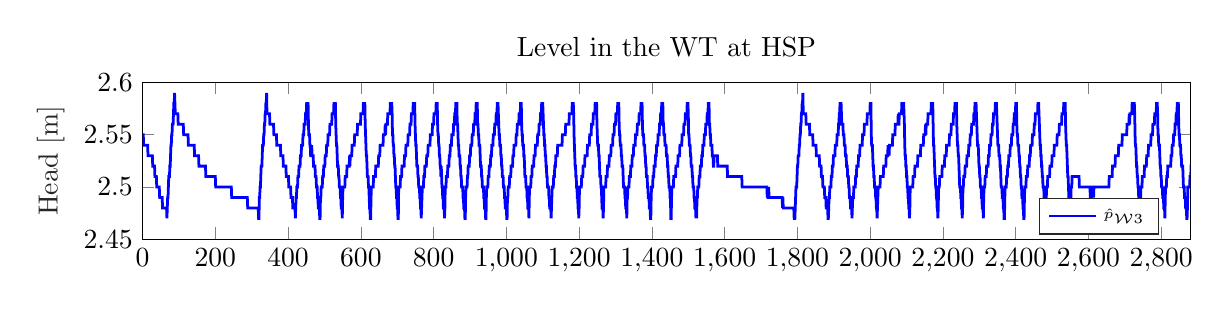
\begin{tikzpicture}

\begin{axis}[%
width=5.239in,
height=0.784in,
at={(1.017in,0.434in)},
scale only axis,
xmin=0,
xmax=2880,
%xlabel style={font=\color{white!15!black}},
%xlabel={Time [min]},
ymin=2.45,
ymax=2.6,
ylabel style={font=\color{white!15!black}},
ylabel={Head  [m]},
axis background/.style={fill=white},
title style={},
title={Level in the WT at HSP},
legend style={at={(0.97,0.03)}, anchor=south east, legend cell align=left, align=left, draw=white!15!black}
]
\addplot [color=blue, line width=1.0pt]
  table[row sep=crcr]{%
0	2.55\\
1	2.55\\
2	2.55\\
3	2.54\\
4	2.54\\
5	2.54\\
6	2.54\\
7	2.54\\
8	2.54\\
9	2.54\\
10	2.54\\
11	2.54\\
12	2.54\\
13	2.54\\
14	2.54\\
15	2.53\\
16	2.53\\
17	2.53\\
18	2.53\\
19	2.53\\
20	2.53\\
21	2.53\\
22	2.53\\
23	2.53\\
24	2.53\\
25	2.53\\
26	2.53\\
27	2.53\\
28	2.52\\
29	2.52\\
30	2.52\\
31	2.52\\
32	2.52\\
33	2.52\\
34	2.51\\
35	2.51\\
36	2.51\\
37	2.51\\
38	2.51\\
39	2.5\\
40	2.5\\
41	2.5\\
42	2.5\\
43	2.5\\
44	2.5\\
45	2.5\\
46	2.5\\
47	2.49\\
48	2.49\\
49	2.49\\
50	2.49\\
51	2.49\\
52	2.49\\
53	2.49\\
54	2.49\\
55	2.48\\
56	2.48\\
57	2.48\\
58	2.48\\
59	2.48\\
60	2.48\\
61	2.48\\
62	2.48\\
63	2.48\\
64	2.48\\
65	2.48\\
66	2.48\\
67	2.47\\
68	2.48\\
69	2.49\\
70	2.49\\
71	2.5\\
72	2.51\\
73	2.51\\
74	2.51\\
75	2.52\\
76	2.52\\
77	2.53\\
78	2.54\\
79	2.54\\
80	2.55\\
81	2.55\\
82	2.56\\
83	2.56\\
84	2.56\\
85	2.57\\
86	2.58\\
87	2.58\\
88	2.59\\
89	2.58\\
90	2.57\\
91	2.57\\
92	2.57\\
93	2.57\\
94	2.57\\
95	2.57\\
96	2.57\\
97	2.57\\
98	2.56\\
99	2.56\\
100	2.56\\
101	2.56\\
102	2.56\\
103	2.56\\
104	2.56\\
105	2.56\\
106	2.56\\
107	2.56\\
108	2.56\\
109	2.56\\
110	2.56\\
111	2.56\\
112	2.56\\
113	2.55\\
114	2.55\\
115	2.55\\
116	2.55\\
117	2.55\\
118	2.55\\
119	2.55\\
120	2.55\\
121	2.55\\
122	2.55\\
123	2.55\\
124	2.55\\
125	2.55\\
126	2.54\\
127	2.54\\
128	2.54\\
129	2.54\\
130	2.54\\
131	2.54\\
132	2.54\\
133	2.54\\
134	2.54\\
135	2.54\\
136	2.54\\
137	2.54\\
138	2.54\\
139	2.54\\
140	2.54\\
141	2.54\\
142	2.54\\
143	2.53\\
144	2.53\\
145	2.53\\
146	2.53\\
147	2.53\\
148	2.53\\
149	2.53\\
150	2.53\\
151	2.53\\
152	2.53\\
153	2.53\\
154	2.53\\
155	2.52\\
156	2.52\\
157	2.52\\
158	2.52\\
159	2.52\\
160	2.52\\
161	2.52\\
162	2.52\\
163	2.52\\
164	2.52\\
165	2.52\\
166	2.52\\
167	2.52\\
168	2.52\\
169	2.52\\
170	2.52\\
171	2.52\\
172	2.52\\
173	2.52\\
174	2.51\\
175	2.51\\
176	2.51\\
177	2.51\\
178	2.51\\
179	2.51\\
180	2.51\\
181	2.51\\
182	2.51\\
183	2.51\\
184	2.51\\
185	2.51\\
186	2.51\\
187	2.51\\
188	2.51\\
189	2.51\\
190	2.51\\
191	2.51\\
192	2.51\\
193	2.51\\
194	2.51\\
195	2.51\\
196	2.51\\
197	2.51\\
198	2.51\\
199	2.51\\
200	2.51\\
201	2.5\\
202	2.5\\
203	2.5\\
204	2.5\\
205	2.5\\
206	2.5\\
207	2.5\\
208	2.5\\
209	2.5\\
210	2.5\\
211	2.5\\
212	2.5\\
213	2.5\\
214	2.5\\
215	2.5\\
216	2.5\\
217	2.5\\
218	2.5\\
219	2.5\\
220	2.5\\
221	2.5\\
222	2.5\\
223	2.5\\
224	2.5\\
225	2.5\\
226	2.5\\
227	2.5\\
228	2.5\\
229	2.5\\
230	2.5\\
231	2.5\\
232	2.5\\
233	2.5\\
234	2.5\\
235	2.5\\
236	2.5\\
237	2.5\\
238	2.5\\
239	2.5\\
240	2.5\\
241	2.5\\
242	2.5\\
243	2.5\\
244	2.5\\
245	2.49\\
246	2.49\\
247	2.49\\
248	2.49\\
249	2.49\\
250	2.49\\
251	2.49\\
252	2.49\\
253	2.49\\
254	2.49\\
255	2.49\\
256	2.49\\
257	2.49\\
258	2.49\\
259	2.49\\
260	2.49\\
261	2.49\\
262	2.49\\
263	2.49\\
264	2.49\\
265	2.49\\
266	2.49\\
267	2.49\\
268	2.49\\
269	2.49\\
270	2.49\\
271	2.49\\
272	2.49\\
273	2.49\\
274	2.49\\
275	2.49\\
276	2.49\\
277	2.49\\
278	2.49\\
279	2.49\\
280	2.49\\
281	2.49\\
282	2.49\\
283	2.49\\
284	2.49\\
285	2.49\\
286	2.49\\
287	2.49\\
288	2.49\\
289	2.48\\
290	2.48\\
291	2.48\\
292	2.48\\
293	2.48\\
294	2.48\\
295	2.48\\
296	2.48\\
297	2.48\\
298	2.48\\
299	2.48\\
300	2.48\\
301	2.48\\
302	2.48\\
303	2.48\\
304	2.48\\
305	2.48\\
306	2.48\\
307	2.48\\
308	2.48\\
309	2.48\\
310	2.48\\
311	2.48\\
312	2.48\\
313	2.48\\
314	2.48\\
315	2.48\\
316	2.48\\
317	2.48\\
318	2.48\\
319	2.47\\
320	2.47\\
321	2.49\\
322	2.49\\
323	2.5\\
324	2.5\\
325	2.51\\
326	2.52\\
327	2.52\\
328	2.52\\
329	2.53\\
330	2.54\\
331	2.54\\
332	2.54\\
333	2.55\\
334	2.55\\
335	2.56\\
336	2.56\\
337	2.57\\
338	2.57\\
339	2.58\\
340	2.58\\
341	2.59\\
342	2.57\\
343	2.57\\
344	2.57\\
345	2.57\\
346	2.57\\
347	2.57\\
348	2.57\\
349	2.57\\
350	2.56\\
351	2.56\\
352	2.56\\
353	2.56\\
354	2.56\\
355	2.56\\
356	2.56\\
357	2.56\\
358	2.56\\
359	2.56\\
360	2.56\\
361	2.55\\
362	2.55\\
363	2.55\\
364	2.55\\
365	2.55\\
366	2.55\\
367	2.55\\
368	2.55\\
369	2.54\\
370	2.54\\
371	2.54\\
372	2.54\\
373	2.54\\
374	2.54\\
375	2.54\\
376	2.54\\
377	2.54\\
378	2.54\\
379	2.54\\
380	2.53\\
381	2.53\\
382	2.53\\
383	2.53\\
384	2.53\\
385	2.53\\
386	2.53\\
387	2.52\\
388	2.52\\
389	2.52\\
390	2.52\\
391	2.52\\
392	2.52\\
393	2.52\\
394	2.52\\
395	2.51\\
396	2.51\\
397	2.51\\
398	2.51\\
399	2.51\\
400	2.51\\
401	2.51\\
402	2.5\\
403	2.5\\
404	2.5\\
405	2.5\\
406	2.5\\
407	2.5\\
408	2.49\\
409	2.49\\
410	2.49\\
411	2.49\\
412	2.49\\
413	2.48\\
414	2.48\\
415	2.48\\
416	2.48\\
417	2.48\\
418	2.48\\
419	2.48\\
420	2.47\\
421	2.48\\
422	2.49\\
423	2.49\\
424	2.5\\
425	2.5\\
426	2.5\\
427	2.51\\
428	2.51\\
429	2.51\\
430	2.52\\
431	2.52\\
432	2.52\\
433	2.52\\
434	2.53\\
435	2.53\\
436	2.53\\
437	2.54\\
438	2.54\\
439	2.54\\
440	2.54\\
441	2.55\\
442	2.55\\
443	2.55\\
444	2.56\\
445	2.56\\
446	2.56\\
447	2.56\\
448	2.57\\
449	2.57\\
450	2.57\\
451	2.58\\
452	2.58\\
453	2.58\\
454	2.58\\
455	2.58\\
456	2.56\\
457	2.55\\
458	2.55\\
459	2.55\\
460	2.54\\
461	2.54\\
462	2.53\\
463	2.53\\
464	2.53\\
465	2.54\\
466	2.53\\
467	2.53\\
468	2.53\\
469	2.53\\
470	2.52\\
471	2.52\\
472	2.52\\
473	2.52\\
474	2.52\\
475	2.51\\
476	2.51\\
477	2.51\\
478	2.5\\
479	2.5\\
480	2.5\\
481	2.49\\
482	2.49\\
483	2.48\\
484	2.48\\
485	2.48\\
486	2.48\\
487	2.47\\
488	2.47\\
489	2.49\\
490	2.49\\
491	2.5\\
492	2.5\\
493	2.5\\
494	2.5\\
495	2.51\\
496	2.51\\
497	2.51\\
498	2.52\\
499	2.52\\
500	2.52\\
501	2.52\\
502	2.53\\
503	2.53\\
504	2.53\\
505	2.53\\
506	2.54\\
507	2.54\\
508	2.54\\
509	2.54\\
510	2.55\\
511	2.55\\
512	2.55\\
513	2.55\\
514	2.55\\
515	2.56\\
516	2.56\\
517	2.56\\
518	2.56\\
519	2.56\\
520	2.56\\
521	2.57\\
522	2.57\\
523	2.57\\
524	2.57\\
525	2.57\\
526	2.58\\
527	2.58\\
528	2.58\\
529	2.58\\
530	2.58\\
531	2.56\\
532	2.55\\
533	2.54\\
534	2.54\\
535	2.53\\
536	2.52\\
537	2.52\\
538	2.52\\
539	2.51\\
540	2.51\\
541	2.5\\
542	2.5\\
543	2.5\\
544	2.49\\
545	2.49\\
546	2.48\\
547	2.48\\
548	2.48\\
549	2.47\\
550	2.49\\
551	2.5\\
552	2.5\\
553	2.5\\
554	2.5\\
555	2.5\\
556	2.5\\
557	2.51\\
558	2.51\\
559	2.51\\
560	2.51\\
561	2.51\\
562	2.52\\
563	2.52\\
564	2.52\\
565	2.52\\
566	2.52\\
567	2.52\\
568	2.52\\
569	2.53\\
570	2.52\\
571	2.53\\
572	2.53\\
573	2.53\\
574	2.53\\
575	2.53\\
576	2.54\\
577	2.54\\
578	2.54\\
579	2.54\\
580	2.54\\
581	2.54\\
582	2.54\\
583	2.55\\
584	2.55\\
585	2.55\\
586	2.55\\
587	2.55\\
588	2.55\\
589	2.55\\
590	2.55\\
591	2.56\\
592	2.56\\
593	2.56\\
594	2.56\\
595	2.56\\
596	2.56\\
597	2.56\\
598	2.56\\
599	2.56\\
600	2.57\\
601	2.57\\
602	2.57\\
603	2.57\\
604	2.57\\
605	2.57\\
606	2.57\\
607	2.58\\
608	2.58\\
609	2.58\\
610	2.58\\
611	2.58\\
612	2.56\\
613	2.55\\
614	2.54\\
615	2.53\\
616	2.53\\
617	2.52\\
618	2.51\\
619	2.51\\
620	2.51\\
621	2.5\\
622	2.5\\
623	2.49\\
624	2.48\\
625	2.48\\
626	2.47\\
627	2.47\\
628	2.49\\
629	2.5\\
630	2.5\\
631	2.5\\
632	2.5\\
633	2.5\\
634	2.5\\
635	2.51\\
636	2.51\\
637	2.51\\
638	2.51\\
639	2.51\\
640	2.51\\
641	2.52\\
642	2.52\\
643	2.52\\
644	2.52\\
645	2.52\\
646	2.52\\
647	2.52\\
648	2.52\\
649	2.53\\
650	2.53\\
651	2.53\\
652	2.53\\
653	2.54\\
654	2.54\\
655	2.54\\
656	2.54\\
657	2.54\\
658	2.54\\
659	2.54\\
660	2.54\\
661	2.54\\
662	2.55\\
663	2.55\\
664	2.55\\
665	2.55\\
666	2.55\\
667	2.56\\
668	2.55\\
669	2.56\\
670	2.56\\
671	2.56\\
672	2.56\\
673	2.56\\
674	2.57\\
675	2.57\\
676	2.57\\
677	2.57\\
678	2.57\\
679	2.57\\
680	2.57\\
681	2.58\\
682	2.58\\
683	2.58\\
684	2.58\\
685	2.58\\
686	2.57\\
687	2.55\\
688	2.55\\
689	2.54\\
690	2.54\\
691	2.53\\
692	2.53\\
693	2.52\\
694	2.52\\
695	2.51\\
696	2.5\\
697	2.5\\
698	2.49\\
699	2.49\\
700	2.48\\
701	2.48\\
702	2.47\\
703	2.47\\
704	2.5\\
705	2.5\\
706	2.5\\
707	2.5\\
708	2.5\\
709	2.51\\
710	2.51\\
711	2.51\\
712	2.51\\
713	2.52\\
714	2.52\\
715	2.52\\
716	2.52\\
717	2.52\\
718	2.52\\
719	2.52\\
720	2.53\\
721	2.53\\
722	2.53\\
723	2.53\\
724	2.54\\
725	2.54\\
726	2.54\\
727	2.54\\
728	2.54\\
729	2.54\\
730	2.55\\
731	2.55\\
732	2.55\\
733	2.55\\
734	2.55\\
735	2.56\\
736	2.56\\
737	2.56\\
738	2.56\\
739	2.57\\
740	2.57\\
741	2.57\\
742	2.57\\
743	2.57\\
744	2.58\\
745	2.58\\
746	2.58\\
747	2.58\\
748	2.58\\
749	2.56\\
750	2.55\\
751	2.54\\
752	2.54\\
753	2.53\\
754	2.52\\
755	2.52\\
756	2.52\\
757	2.51\\
758	2.51\\
759	2.5\\
760	2.5\\
761	2.5\\
762	2.49\\
763	2.49\\
764	2.48\\
765	2.48\\
766	2.47\\
767	2.48\\
768	2.49\\
769	2.5\\
770	2.5\\
771	2.5\\
772	2.5\\
773	2.51\\
774	2.51\\
775	2.51\\
776	2.52\\
777	2.52\\
778	2.52\\
779	2.52\\
780	2.52\\
781	2.53\\
782	2.53\\
783	2.53\\
784	2.53\\
785	2.54\\
786	2.54\\
787	2.54\\
788	2.54\\
789	2.54\\
790	2.54\\
791	2.55\\
792	2.55\\
793	2.55\\
794	2.55\\
795	2.55\\
796	2.55\\
797	2.56\\
798	2.56\\
799	2.56\\
800	2.56\\
801	2.57\\
802	2.57\\
803	2.57\\
804	2.57\\
805	2.57\\
806	2.57\\
807	2.58\\
808	2.58\\
809	2.58\\
810	2.58\\
811	2.56\\
812	2.55\\
813	2.55\\
814	2.54\\
815	2.54\\
816	2.53\\
817	2.53\\
818	2.52\\
819	2.52\\
820	2.51\\
821	2.52\\
822	2.51\\
823	2.5\\
824	2.5\\
825	2.49\\
826	2.49\\
827	2.48\\
828	2.48\\
829	2.48\\
830	2.47\\
831	2.48\\
832	2.5\\
833	2.5\\
834	2.5\\
835	2.51\\
836	2.51\\
837	2.51\\
838	2.51\\
839	2.52\\
840	2.52\\
841	2.52\\
842	2.52\\
843	2.53\\
844	2.53\\
845	2.53\\
846	2.54\\
847	2.54\\
848	2.54\\
849	2.54\\
850	2.55\\
851	2.55\\
852	2.55\\
853	2.55\\
854	2.55\\
855	2.56\\
856	2.56\\
857	2.56\\
858	2.57\\
859	2.57\\
860	2.57\\
861	2.58\\
862	2.58\\
863	2.58\\
864	2.58\\
865	2.56\\
866	2.56\\
867	2.55\\
868	2.54\\
869	2.54\\
870	2.53\\
871	2.53\\
872	2.53\\
873	2.52\\
874	2.52\\
875	2.51\\
876	2.51\\
877	2.5\\
878	2.5\\
879	2.5\\
880	2.5\\
881	2.49\\
882	2.49\\
883	2.48\\
884	2.48\\
885	2.48\\
886	2.47\\
887	2.47\\
888	2.49\\
889	2.5\\
890	2.5\\
891	2.5\\
892	2.5\\
893	2.51\\
894	2.51\\
895	2.52\\
896	2.52\\
897	2.52\\
898	2.52\\
899	2.53\\
900	2.53\\
901	2.53\\
902	2.54\\
903	2.54\\
904	2.54\\
905	2.54\\
906	2.55\\
907	2.55\\
908	2.55\\
909	2.55\\
910	2.56\\
911	2.56\\
912	2.56\\
913	2.56\\
914	2.57\\
915	2.57\\
916	2.57\\
917	2.58\\
918	2.58\\
919	2.58\\
920	2.58\\
921	2.56\\
922	2.56\\
923	2.55\\
924	2.55\\
925	2.54\\
926	2.54\\
927	2.54\\
928	2.53\\
929	2.52\\
930	2.52\\
931	2.52\\
932	2.51\\
933	2.51\\
934	2.5\\
935	2.5\\
936	2.5\\
937	2.5\\
938	2.49\\
939	2.49\\
940	2.48\\
941	2.48\\
942	2.48\\
943	2.47\\
944	2.47\\
945	2.49\\
946	2.5\\
947	2.5\\
948	2.5\\
949	2.5\\
950	2.51\\
951	2.51\\
952	2.51\\
953	2.52\\
954	2.52\\
955	2.52\\
956	2.52\\
957	2.53\\
958	2.53\\
959	2.53\\
960	2.54\\
961	2.54\\
962	2.54\\
963	2.54\\
964	2.55\\
965	2.55\\
966	2.55\\
967	2.55\\
968	2.56\\
969	2.56\\
970	2.56\\
971	2.56\\
972	2.57\\
973	2.57\\
974	2.57\\
975	2.58\\
976	2.58\\
977	2.58\\
978	2.57\\
979	2.56\\
980	2.55\\
981	2.55\\
982	2.54\\
983	2.54\\
984	2.54\\
985	2.53\\
986	2.53\\
987	2.52\\
988	2.52\\
989	2.51\\
990	2.51\\
991	2.51\\
992	2.5\\
993	2.5\\
994	2.5\\
995	2.49\\
996	2.49\\
997	2.48\\
998	2.48\\
999	2.48\\
1000	2.48\\
1001	2.47\\
1002	2.47\\
1003	2.49\\
1004	2.49\\
1005	2.5\\
1006	2.5\\
1007	2.5\\
1008	2.5\\
1009	2.51\\
1010	2.51\\
1011	2.51\\
1012	2.51\\
1013	2.52\\
1014	2.52\\
1015	2.52\\
1016	2.52\\
1017	2.52\\
1018	2.53\\
1019	2.53\\
1020	2.53\\
1021	2.54\\
1022	2.54\\
1023	2.54\\
1024	2.54\\
1025	2.54\\
1026	2.54\\
1027	2.55\\
1028	2.55\\
1029	2.55\\
1030	2.56\\
1031	2.56\\
1032	2.56\\
1033	2.56\\
1034	2.56\\
1035	2.57\\
1036	2.57\\
1037	2.57\\
1038	2.57\\
1039	2.58\\
1040	2.58\\
1041	2.58\\
1042	2.56\\
1043	2.55\\
1044	2.55\\
1045	2.54\\
1046	2.54\\
1047	2.54\\
1048	2.53\\
1049	2.53\\
1050	2.52\\
1051	2.51\\
1052	2.51\\
1053	2.51\\
1054	2.5\\
1055	2.5\\
1056	2.5\\
1057	2.49\\
1058	2.49\\
1059	2.48\\
1060	2.48\\
1061	2.48\\
1062	2.47\\
1063	2.49\\
1064	2.5\\
1065	2.5\\
1066	2.5\\
1067	2.5\\
1068	2.51\\
1069	2.51\\
1070	2.51\\
1071	2.52\\
1072	2.52\\
1073	2.52\\
1074	2.52\\
1075	2.52\\
1076	2.53\\
1077	2.53\\
1078	2.53\\
1079	2.53\\
1080	2.54\\
1081	2.54\\
1082	2.54\\
1083	2.54\\
1084	2.54\\
1085	2.54\\
1086	2.55\\
1087	2.55\\
1088	2.55\\
1089	2.55\\
1090	2.56\\
1091	2.56\\
1092	2.56\\
1093	2.56\\
1094	2.57\\
1095	2.57\\
1096	2.57\\
1097	2.58\\
1098	2.58\\
1099	2.58\\
1100	2.58\\
1101	2.57\\
1102	2.56\\
1103	2.55\\
1104	2.55\\
1105	2.54\\
1106	2.54\\
1107	2.53\\
1108	2.53\\
1109	2.52\\
1110	2.52\\
1111	2.51\\
1112	2.51\\
1113	2.5\\
1114	2.5\\
1115	2.5\\
1116	2.5\\
1117	2.49\\
1118	2.49\\
1119	2.48\\
1120	2.48\\
1121	2.48\\
1122	2.48\\
1123	2.47\\
1124	2.48\\
1125	2.49\\
1126	2.5\\
1127	2.5\\
1128	2.5\\
1129	2.5\\
1130	2.51\\
1131	2.51\\
1132	2.51\\
1133	2.52\\
1134	2.52\\
1135	2.52\\
1136	2.53\\
1137	2.53\\
1138	2.53\\
1139	2.53\\
1140	2.53\\
1141	2.54\\
1142	2.54\\
1143	2.54\\
1144	2.54\\
1145	2.54\\
1146	2.54\\
1147	2.54\\
1148	2.54\\
1149	2.54\\
1150	2.54\\
1151	2.54\\
1152	2.54\\
1153	2.54\\
1154	2.55\\
1155	2.55\\
1156	2.55\\
1157	2.55\\
1158	2.55\\
1159	2.55\\
1160	2.55\\
1161	2.55\\
1162	2.55\\
1163	2.56\\
1164	2.56\\
1165	2.56\\
1166	2.56\\
1167	2.56\\
1168	2.56\\
1169	2.56\\
1170	2.56\\
1171	2.56\\
1172	2.56\\
1173	2.57\\
1174	2.57\\
1175	2.57\\
1176	2.57\\
1177	2.57\\
1178	2.57\\
1179	2.57\\
1180	2.57\\
1181	2.58\\
1182	2.58\\
1183	2.58\\
1184	2.58\\
1185	2.57\\
1186	2.55\\
1187	2.54\\
1188	2.53\\
1189	2.52\\
1190	2.52\\
1191	2.51\\
1192	2.51\\
1193	2.5\\
1194	2.5\\
1195	2.49\\
1196	2.49\\
1197	2.48\\
1198	2.48\\
1199	2.47\\
1200	2.48\\
1201	2.5\\
1202	2.5\\
1203	2.5\\
1204	2.5\\
1205	2.5\\
1206	2.5\\
1207	2.51\\
1208	2.51\\
1209	2.51\\
1210	2.51\\
1211	2.52\\
1212	2.52\\
1213	2.52\\
1214	2.52\\
1215	2.52\\
1216	2.53\\
1217	2.53\\
1218	2.53\\
1219	2.53\\
1220	2.53\\
1221	2.53\\
1222	2.53\\
1223	2.54\\
1224	2.54\\
1225	2.54\\
1226	2.54\\
1227	2.54\\
1228	2.54\\
1229	2.55\\
1230	2.55\\
1231	2.55\\
1232	2.55\\
1233	2.55\\
1234	2.56\\
1235	2.56\\
1236	2.56\\
1237	2.56\\
1238	2.56\\
1239	2.57\\
1240	2.57\\
1241	2.57\\
1242	2.57\\
1243	2.57\\
1244	2.58\\
1245	2.58\\
1246	2.58\\
1247	2.58\\
1248	2.58\\
1249	2.56\\
1250	2.55\\
1251	2.54\\
1252	2.54\\
1253	2.54\\
1254	2.53\\
1255	2.53\\
1256	2.52\\
1257	2.51\\
1258	2.51\\
1259	2.51\\
1260	2.5\\
1261	2.5\\
1262	2.49\\
1263	2.48\\
1264	2.48\\
1265	2.48\\
1266	2.47\\
1267	2.48\\
1268	2.5\\
1269	2.5\\
1270	2.5\\
1271	2.5\\
1272	2.5\\
1273	2.5\\
1274	2.51\\
1275	2.51\\
1276	2.51\\
1277	2.51\\
1278	2.52\\
1279	2.52\\
1280	2.52\\
1281	2.52\\
1282	2.52\\
1283	2.53\\
1284	2.53\\
1285	2.53\\
1286	2.53\\
1287	2.53\\
1288	2.54\\
1289	2.54\\
1290	2.54\\
1291	2.54\\
1292	2.54\\
1293	2.55\\
1294	2.55\\
1295	2.55\\
1296	2.55\\
1297	2.56\\
1298	2.56\\
1299	2.56\\
1300	2.56\\
1301	2.57\\
1302	2.57\\
1303	2.57\\
1304	2.57\\
1305	2.57\\
1306	2.58\\
1307	2.58\\
1308	2.58\\
1309	2.58\\
1310	2.56\\
1311	2.55\\
1312	2.55\\
1313	2.54\\
1314	2.54\\
1315	2.54\\
1316	2.53\\
1317	2.53\\
1318	2.52\\
1319	2.52\\
1320	2.52\\
1321	2.51\\
1322	2.5\\
1323	2.5\\
1324	2.5\\
1325	2.5\\
1326	2.49\\
1327	2.49\\
1328	2.48\\
1329	2.48\\
1330	2.48\\
1331	2.47\\
1332	2.49\\
1333	2.49\\
1334	2.5\\
1335	2.5\\
1336	2.5\\
1337	2.5\\
1338	2.51\\
1339	2.51\\
1340	2.51\\
1341	2.51\\
1342	2.52\\
1343	2.52\\
1344	2.52\\
1345	2.52\\
1346	2.53\\
1347	2.53\\
1348	2.53\\
1349	2.53\\
1350	2.54\\
1351	2.54\\
1352	2.54\\
1353	2.54\\
1354	2.54\\
1355	2.55\\
1356	2.55\\
1357	2.55\\
1358	2.55\\
1359	2.55\\
1360	2.56\\
1361	2.56\\
1362	2.56\\
1363	2.56\\
1364	2.56\\
1365	2.57\\
1366	2.57\\
1367	2.57\\
1368	2.57\\
1369	2.57\\
1370	2.58\\
1371	2.58\\
1372	2.58\\
1373	2.58\\
1374	2.56\\
1375	2.55\\
1376	2.55\\
1377	2.55\\
1378	2.54\\
1379	2.54\\
1380	2.54\\
1381	2.53\\
1382	2.53\\
1383	2.52\\
1384	2.52\\
1385	2.51\\
1386	2.51\\
1387	2.51\\
1388	2.5\\
1389	2.5\\
1390	2.49\\
1391	2.49\\
1392	2.49\\
1393	2.48\\
1394	2.48\\
1395	2.48\\
1396	2.47\\
1397	2.47\\
1398	2.49\\
1399	2.5\\
1400	2.5\\
1401	2.5\\
1402	2.5\\
1403	2.51\\
1404	2.51\\
1405	2.51\\
1406	2.52\\
1407	2.52\\
1408	2.52\\
1409	2.52\\
1410	2.53\\
1411	2.53\\
1412	2.53\\
1413	2.54\\
1414	2.54\\
1415	2.54\\
1416	2.54\\
1417	2.55\\
1418	2.55\\
1419	2.55\\
1420	2.55\\
1421	2.56\\
1422	2.56\\
1423	2.56\\
1424	2.57\\
1425	2.57\\
1426	2.57\\
1427	2.58\\
1428	2.58\\
1429	2.58\\
1430	2.58\\
1431	2.56\\
1432	2.56\\
1433	2.55\\
1434	2.55\\
1435	2.55\\
1436	2.54\\
1437	2.54\\
1438	2.54\\
1439	2.54\\
1440	2.53\\
1441	2.53\\
1442	2.53\\
1443	2.52\\
1444	2.52\\
1445	2.51\\
1446	2.51\\
1447	2.5\\
1448	2.5\\
1449	2.5\\
1450	2.49\\
1451	2.49\\
1452	2.47\\
1453	2.47\\
1454	2.49\\
1455	2.5\\
1456	2.5\\
1457	2.5\\
1458	2.5\\
1459	2.5\\
1460	2.51\\
1461	2.51\\
1462	2.51\\
1463	2.51\\
1464	2.51\\
1465	2.51\\
1466	2.52\\
1467	2.52\\
1468	2.52\\
1469	2.52\\
1470	2.52\\
1471	2.52\\
1472	2.53\\
1473	2.53\\
1474	2.53\\
1475	2.53\\
1476	2.53\\
1477	2.54\\
1478	2.54\\
1479	2.54\\
1480	2.54\\
1481	2.54\\
1482	2.54\\
1483	2.55\\
1484	2.55\\
1485	2.55\\
1486	2.55\\
1487	2.55\\
1488	2.56\\
1489	2.56\\
1490	2.56\\
1491	2.56\\
1492	2.57\\
1493	2.57\\
1494	2.57\\
1495	2.57\\
1496	2.57\\
1497	2.58\\
1498	2.58\\
1499	2.58\\
1500	2.57\\
1501	2.55\\
1502	2.55\\
1503	2.54\\
1504	2.54\\
1505	2.54\\
1506	2.53\\
1507	2.53\\
1508	2.52\\
1509	2.52\\
1510	2.52\\
1511	2.51\\
1512	2.51\\
1513	2.5\\
1514	2.5\\
1515	2.5\\
1516	2.49\\
1517	2.49\\
1518	2.48\\
1519	2.48\\
1520	2.48\\
1521	2.47\\
1522	2.48\\
1523	2.47\\
1524	2.49\\
1525	2.49\\
1526	2.5\\
1527	2.5\\
1528	2.5\\
1529	2.5\\
1530	2.51\\
1531	2.51\\
1532	2.51\\
1533	2.52\\
1534	2.52\\
1535	2.52\\
1536	2.52\\
1537	2.53\\
1538	2.53\\
1539	2.53\\
1540	2.54\\
1541	2.54\\
1542	2.54\\
1543	2.54\\
1544	2.55\\
1545	2.55\\
1546	2.55\\
1547	2.55\\
1548	2.56\\
1549	2.56\\
1550	2.56\\
1551	2.56\\
1552	2.57\\
1553	2.57\\
1554	2.57\\
1555	2.58\\
1556	2.58\\
1557	2.58\\
1558	2.56\\
1559	2.56\\
1560	2.55\\
1561	2.55\\
1562	2.54\\
1563	2.54\\
1564	2.54\\
1565	2.54\\
1566	2.53\\
1567	2.53\\
1568	2.53\\
1569	2.52\\
1570	2.52\\
1571	2.53\\
1572	2.53\\
1573	2.53\\
1574	2.53\\
1575	2.53\\
1576	2.53\\
1577	2.53\\
1578	2.53\\
1579	2.53\\
1580	2.53\\
1581	2.52\\
1582	2.52\\
1583	2.52\\
1584	2.52\\
1585	2.52\\
1586	2.52\\
1587	2.52\\
1588	2.52\\
1589	2.52\\
1590	2.52\\
1591	2.52\\
1592	2.52\\
1593	2.52\\
1594	2.52\\
1595	2.52\\
1596	2.52\\
1597	2.52\\
1598	2.52\\
1599	2.52\\
1600	2.52\\
1601	2.52\\
1602	2.52\\
1603	2.52\\
1604	2.52\\
1605	2.52\\
1606	2.52\\
1607	2.52\\
1608	2.51\\
1609	2.51\\
1610	2.51\\
1611	2.51\\
1612	2.51\\
1613	2.51\\
1614	2.51\\
1615	2.51\\
1616	2.51\\
1617	2.51\\
1618	2.51\\
1619	2.51\\
1620	2.51\\
1621	2.51\\
1622	2.51\\
1623	2.51\\
1624	2.51\\
1625	2.51\\
1626	2.51\\
1627	2.51\\
1628	2.51\\
1629	2.51\\
1630	2.51\\
1631	2.51\\
1632	2.51\\
1633	2.51\\
1634	2.51\\
1635	2.51\\
1636	2.51\\
1637	2.51\\
1638	2.51\\
1639	2.51\\
1640	2.51\\
1641	2.51\\
1642	2.51\\
1643	2.51\\
1644	2.51\\
1645	2.51\\
1646	2.51\\
1647	2.51\\
1648	2.5\\
1649	2.5\\
1650	2.5\\
1651	2.5\\
1652	2.5\\
1653	2.5\\
1654	2.5\\
1655	2.5\\
1656	2.5\\
1657	2.5\\
1658	2.5\\
1659	2.5\\
1660	2.5\\
1661	2.5\\
1662	2.5\\
1663	2.5\\
1664	2.5\\
1665	2.5\\
1666	2.5\\
1667	2.5\\
1668	2.5\\
1669	2.5\\
1670	2.5\\
1671	2.5\\
1672	2.5\\
1673	2.5\\
1674	2.5\\
1675	2.5\\
1676	2.5\\
1677	2.5\\
1678	2.5\\
1679	2.5\\
1680	2.5\\
1681	2.5\\
1682	2.5\\
1683	2.5\\
1684	2.5\\
1685	2.5\\
1686	2.5\\
1687	2.5\\
1688	2.5\\
1689	2.5\\
1690	2.5\\
1691	2.5\\
1692	2.5\\
1693	2.5\\
1694	2.5\\
1695	2.5\\
1696	2.5\\
1697	2.5\\
1698	2.5\\
1699	2.5\\
1700	2.5\\
1701	2.5\\
1702	2.5\\
1703	2.5\\
1704	2.5\\
1705	2.5\\
1706	2.5\\
1707	2.5\\
1708	2.5\\
1709	2.5\\
1710	2.5\\
1711	2.5\\
1712	2.5\\
1713	2.5\\
1714	2.5\\
1715	2.5\\
1716	2.5\\
1717	2.49\\
1718	2.5\\
1719	2.49\\
1720	2.49\\
1721	2.5\\
1722	2.49\\
1723	2.49\\
1724	2.49\\
1725	2.49\\
1726	2.49\\
1727	2.49\\
1728	2.49\\
1729	2.49\\
1730	2.49\\
1731	2.49\\
1732	2.49\\
1733	2.49\\
1734	2.49\\
1735	2.49\\
1736	2.49\\
1737	2.49\\
1738	2.49\\
1739	2.49\\
1740	2.49\\
1741	2.49\\
1742	2.49\\
1743	2.49\\
1744	2.49\\
1745	2.49\\
1746	2.49\\
1747	2.49\\
1748	2.49\\
1749	2.49\\
1750	2.49\\
1751	2.49\\
1752	2.49\\
1753	2.49\\
1754	2.49\\
1755	2.49\\
1756	2.49\\
1757	2.49\\
1758	2.49\\
1759	2.48\\
1760	2.49\\
1761	2.48\\
1762	2.48\\
1763	2.48\\
1764	2.48\\
1765	2.48\\
1766	2.48\\
1767	2.48\\
1768	2.48\\
1769	2.48\\
1770	2.48\\
1771	2.48\\
1772	2.48\\
1773	2.48\\
1774	2.48\\
1775	2.48\\
1776	2.48\\
1777	2.48\\
1778	2.48\\
1779	2.48\\
1780	2.48\\
1781	2.48\\
1782	2.48\\
1783	2.48\\
1784	2.48\\
1785	2.48\\
1786	2.48\\
1787	2.48\\
1788	2.48\\
1789	2.48\\
1790	2.48\\
1791	2.47\\
1792	2.47\\
1793	2.47\\
1794	2.48\\
1795	2.49\\
1796	2.5\\
1797	2.5\\
1798	2.5\\
1799	2.51\\
1800	2.52\\
1801	2.52\\
1802	2.53\\
1803	2.53\\
1804	2.53\\
1805	2.54\\
1806	2.54\\
1807	2.55\\
1808	2.55\\
1809	2.56\\
1810	2.56\\
1811	2.57\\
1812	2.57\\
1813	2.58\\
1814	2.58\\
1815	2.59\\
1816	2.57\\
1817	2.57\\
1818	2.57\\
1819	2.57\\
1820	2.57\\
1821	2.57\\
1822	2.57\\
1823	2.57\\
1824	2.56\\
1825	2.56\\
1826	2.56\\
1827	2.56\\
1828	2.56\\
1829	2.56\\
1830	2.56\\
1831	2.56\\
1832	2.56\\
1833	2.56\\
1834	2.55\\
1835	2.55\\
1836	2.55\\
1837	2.55\\
1838	2.55\\
1839	2.55\\
1840	2.55\\
1841	2.55\\
1842	2.55\\
1843	2.54\\
1844	2.54\\
1845	2.54\\
1846	2.54\\
1847	2.54\\
1848	2.54\\
1849	2.54\\
1850	2.54\\
1851	2.54\\
1852	2.53\\
1853	2.53\\
1854	2.53\\
1855	2.53\\
1856	2.53\\
1857	2.53\\
1858	2.53\\
1859	2.53\\
1860	2.53\\
1861	2.52\\
1862	2.52\\
1863	2.52\\
1864	2.52\\
1865	2.52\\
1866	2.51\\
1867	2.51\\
1868	2.51\\
1869	2.51\\
1870	2.5\\
1871	2.5\\
1872	2.5\\
1873	2.5\\
1874	2.5\\
1875	2.49\\
1876	2.49\\
1877	2.49\\
1878	2.49\\
1879	2.48\\
1880	2.48\\
1881	2.48\\
1882	2.48\\
1883	2.48\\
1884	2.47\\
1885	2.47\\
1886	2.48\\
1887	2.49\\
1888	2.49\\
1889	2.5\\
1890	2.5\\
1891	2.5\\
1892	2.5\\
1893	2.51\\
1894	2.51\\
1895	2.51\\
1896	2.52\\
1897	2.52\\
1898	2.52\\
1899	2.53\\
1900	2.53\\
1901	2.53\\
1902	2.53\\
1903	2.53\\
1904	2.54\\
1905	2.54\\
1906	2.54\\
1907	2.54\\
1908	2.54\\
1909	2.55\\
1910	2.55\\
1911	2.55\\
1912	2.55\\
1913	2.56\\
1914	2.56\\
1915	2.57\\
1916	2.57\\
1917	2.58\\
1918	2.58\\
1919	2.58\\
1920	2.58\\
1921	2.57\\
1922	2.56\\
1923	2.56\\
1924	2.56\\
1925	2.56\\
1926	2.55\\
1927	2.55\\
1928	2.55\\
1929	2.54\\
1930	2.54\\
1931	2.54\\
1932	2.53\\
1933	2.53\\
1934	2.53\\
1935	2.52\\
1936	2.52\\
1937	2.52\\
1938	2.51\\
1939	2.51\\
1940	2.51\\
1941	2.5\\
1942	2.5\\
1943	2.49\\
1944	2.49\\
1945	2.49\\
1946	2.48\\
1947	2.48\\
1948	2.48\\
1949	2.48\\
1950	2.47\\
1951	2.48\\
1952	2.49\\
1953	2.49\\
1954	2.49\\
1955	2.5\\
1956	2.5\\
1957	2.5\\
1958	2.5\\
1959	2.5\\
1960	2.51\\
1961	2.51\\
1962	2.51\\
1963	2.52\\
1964	2.52\\
1965	2.52\\
1966	2.52\\
1967	2.52\\
1968	2.53\\
1969	2.53\\
1970	2.53\\
1971	2.53\\
1972	2.54\\
1973	2.54\\
1974	2.54\\
1975	2.54\\
1976	2.54\\
1977	2.54\\
1978	2.54\\
1979	2.55\\
1980	2.55\\
1981	2.55\\
1982	2.55\\
1983	2.55\\
1984	2.56\\
1985	2.56\\
1986	2.56\\
1987	2.56\\
1988	2.56\\
1989	2.56\\
1990	2.56\\
1991	2.56\\
1992	2.57\\
1993	2.57\\
1994	2.57\\
1995	2.57\\
1996	2.57\\
1997	2.57\\
1998	2.57\\
1999	2.57\\
2000	2.58\\
2001	2.58\\
2002	2.58\\
2003	2.55\\
2004	2.54\\
2005	2.54\\
2006	2.54\\
2007	2.53\\
2008	2.52\\
2009	2.52\\
2010	2.51\\
2011	2.51\\
2012	2.5\\
2013	2.5\\
2014	2.5\\
2015	2.49\\
2016	2.49\\
2017	2.48\\
2018	2.48\\
2019	2.47\\
2020	2.48\\
2021	2.49\\
2022	2.5\\
2023	2.5\\
2024	2.5\\
2025	2.5\\
2026	2.5\\
2027	2.5\\
2028	2.51\\
2029	2.51\\
2030	2.51\\
2031	2.51\\
2032	2.51\\
2033	2.51\\
2034	2.51\\
2035	2.51\\
2036	2.51\\
2037	2.52\\
2038	2.52\\
2039	2.52\\
2040	2.52\\
2041	2.52\\
2042	2.52\\
2043	2.52\\
2044	2.53\\
2045	2.53\\
2046	2.53\\
2047	2.53\\
2048	2.53\\
2049	2.54\\
2050	2.53\\
2051	2.54\\
2052	2.53\\
2053	2.54\\
2054	2.54\\
2055	2.54\\
2056	2.54\\
2057	2.54\\
2058	2.54\\
2059	2.54\\
2060	2.54\\
2061	2.54\\
2062	2.55\\
2063	2.55\\
2064	2.55\\
2065	2.55\\
2066	2.55\\
2067	2.55\\
2068	2.55\\
2069	2.56\\
2070	2.56\\
2071	2.56\\
2072	2.56\\
2073	2.56\\
2074	2.56\\
2075	2.56\\
2076	2.56\\
2077	2.57\\
2078	2.56\\
2079	2.56\\
2080	2.57\\
2081	2.57\\
2082	2.57\\
2083	2.57\\
2084	2.57\\
2085	2.57\\
2086	2.57\\
2087	2.58\\
2088	2.58\\
2089	2.58\\
2090	2.58\\
2091	2.58\\
2092	2.58\\
2093	2.57\\
2094	2.56\\
2095	2.54\\
2096	2.53\\
2097	2.53\\
2098	2.52\\
2099	2.52\\
2100	2.51\\
2101	2.51\\
2102	2.5\\
2103	2.5\\
2104	2.49\\
2105	2.49\\
2106	2.48\\
2107	2.48\\
2108	2.47\\
2109	2.48\\
2110	2.5\\
2111	2.5\\
2112	2.5\\
2113	2.5\\
2114	2.5\\
2115	2.5\\
2116	2.5\\
2117	2.5\\
2118	2.51\\
2119	2.51\\
2120	2.51\\
2121	2.51\\
2122	2.51\\
2123	2.52\\
2124	2.52\\
2125	2.52\\
2126	2.52\\
2127	2.52\\
2128	2.52\\
2129	2.52\\
2130	2.52\\
2131	2.53\\
2132	2.53\\
2133	2.53\\
2134	2.53\\
2135	2.53\\
2136	2.53\\
2137	2.53\\
2138	2.53\\
2139	2.54\\
2140	2.54\\
2141	2.54\\
2142	2.54\\
2143	2.54\\
2144	2.54\\
2145	2.54\\
2146	2.54\\
2147	2.55\\
2148	2.55\\
2149	2.55\\
2150	2.55\\
2151	2.55\\
2152	2.56\\
2153	2.55\\
2154	2.56\\
2155	2.56\\
2156	2.56\\
2157	2.56\\
2158	2.56\\
2159	2.57\\
2160	2.57\\
2161	2.57\\
2162	2.57\\
2163	2.57\\
2164	2.57\\
2165	2.57\\
2166	2.57\\
2167	2.57\\
2168	2.58\\
2169	2.58\\
2170	2.58\\
2171	2.58\\
2172	2.58\\
2173	2.56\\
2174	2.54\\
2175	2.54\\
2176	2.53\\
2177	2.52\\
2178	2.51\\
2179	2.51\\
2180	2.5\\
2181	2.5\\
2182	2.49\\
2183	2.49\\
2184	2.48\\
2185	2.48\\
2186	2.47\\
2187	2.48\\
2188	2.5\\
2189	2.5\\
2190	2.5\\
2191	2.51\\
2192	2.51\\
2193	2.51\\
2194	2.51\\
2195	2.51\\
2196	2.51\\
2197	2.51\\
2198	2.52\\
2199	2.52\\
2200	2.52\\
2201	2.52\\
2202	2.52\\
2203	2.52\\
2204	2.52\\
2205	2.53\\
2206	2.53\\
2207	2.53\\
2208	2.53\\
2209	2.53\\
2210	2.54\\
2211	2.54\\
2212	2.54\\
2213	2.54\\
2214	2.54\\
2215	2.54\\
2216	2.54\\
2217	2.54\\
2218	2.55\\
2219	2.55\\
2220	2.55\\
2221	2.55\\
2222	2.55\\
2223	2.56\\
2224	2.56\\
2225	2.56\\
2226	2.56\\
2227	2.56\\
2228	2.56\\
2229	2.57\\
2230	2.57\\
2231	2.57\\
2232	2.57\\
2233	2.58\\
2234	2.58\\
2235	2.58\\
2236	2.58\\
2237	2.58\\
2238	2.56\\
2239	2.55\\
2240	2.54\\
2241	2.54\\
2242	2.53\\
2243	2.53\\
2244	2.52\\
2245	2.51\\
2246	2.5\\
2247	2.5\\
2248	2.5\\
2249	2.49\\
2250	2.49\\
2251	2.48\\
2252	2.48\\
2253	2.47\\
2254	2.48\\
2255	2.5\\
2256	2.5\\
2257	2.51\\
2258	2.51\\
2259	2.51\\
2260	2.51\\
2261	2.52\\
2262	2.52\\
2263	2.52\\
2264	2.52\\
2265	2.52\\
2266	2.53\\
2267	2.53\\
2268	2.53\\
2269	2.53\\
2270	2.53\\
2271	2.54\\
2272	2.54\\
2273	2.54\\
2274	2.54\\
2275	2.55\\
2276	2.55\\
2277	2.55\\
2278	2.55\\
2279	2.56\\
2280	2.56\\
2281	2.56\\
2282	2.56\\
2283	2.56\\
2284	2.56\\
2285	2.57\\
2286	2.57\\
2287	2.57\\
2288	2.58\\
2289	2.58\\
2290	2.58\\
2291	2.58\\
2292	2.57\\
2293	2.56\\
2294	2.55\\
2295	2.54\\
2296	2.54\\
2297	2.54\\
2298	2.53\\
2299	2.52\\
2300	2.52\\
2301	2.51\\
2302	2.51\\
2303	2.5\\
2304	2.5\\
2305	2.5\\
2306	2.49\\
2307	2.49\\
2308	2.48\\
2309	2.48\\
2310	2.48\\
2311	2.47\\
2312	2.49\\
2313	2.5\\
2314	2.5\\
2315	2.5\\
2316	2.51\\
2317	2.51\\
2318	2.51\\
2319	2.51\\
2320	2.52\\
2321	2.52\\
2322	2.52\\
2323	2.52\\
2324	2.52\\
2325	2.53\\
2326	2.53\\
2327	2.53\\
2328	2.54\\
2329	2.54\\
2330	2.54\\
2331	2.54\\
2332	2.55\\
2333	2.55\\
2334	2.55\\
2335	2.55\\
2336	2.56\\
2337	2.56\\
2338	2.56\\
2339	2.57\\
2340	2.57\\
2341	2.57\\
2342	2.57\\
2343	2.57\\
2344	2.58\\
2345	2.58\\
2346	2.58\\
2347	2.58\\
2348	2.57\\
2349	2.56\\
2350	2.55\\
2351	2.54\\
2352	2.54\\
2353	2.54\\
2354	2.53\\
2355	2.53\\
2356	2.53\\
2357	2.52\\
2358	2.52\\
2359	2.51\\
2360	2.5\\
2361	2.5\\
2362	2.5\\
2363	2.49\\
2364	2.49\\
2365	2.49\\
2366	2.48\\
2367	2.48\\
2368	2.47\\
2369	2.47\\
2370	2.49\\
2371	2.5\\
2372	2.5\\
2373	2.5\\
2374	2.5\\
2375	2.51\\
2376	2.51\\
2377	2.51\\
2378	2.52\\
2379	2.52\\
2380	2.52\\
2381	2.53\\
2382	2.53\\
2383	2.53\\
2384	2.53\\
2385	2.54\\
2386	2.54\\
2387	2.54\\
2388	2.54\\
2389	2.55\\
2390	2.55\\
2391	2.55\\
2392	2.55\\
2393	2.56\\
2394	2.56\\
2395	2.56\\
2396	2.57\\
2397	2.57\\
2398	2.57\\
2399	2.57\\
2400	2.58\\
2401	2.58\\
2402	2.58\\
2403	2.56\\
2404	2.55\\
2405	2.55\\
2406	2.54\\
2407	2.54\\
2408	2.54\\
2409	2.53\\
2410	2.53\\
2411	2.52\\
2412	2.52\\
2413	2.51\\
2414	2.51\\
2415	2.5\\
2416	2.5\\
2417	2.49\\
2418	2.49\\
2419	2.49\\
2420	2.48\\
2421	2.48\\
2422	2.47\\
2423	2.47\\
2424	2.49\\
2425	2.5\\
2426	2.5\\
2427	2.5\\
2428	2.5\\
2429	2.51\\
2430	2.51\\
2431	2.51\\
2432	2.51\\
2433	2.52\\
2434	2.52\\
2435	2.52\\
2436	2.52\\
2437	2.52\\
2438	2.53\\
2439	2.53\\
2440	2.53\\
2441	2.54\\
2442	2.54\\
2443	2.54\\
2444	2.54\\
2445	2.54\\
2446	2.55\\
2447	2.55\\
2448	2.55\\
2449	2.55\\
2450	2.55\\
2451	2.56\\
2452	2.56\\
2453	2.56\\
2454	2.57\\
2455	2.57\\
2456	2.57\\
2457	2.57\\
2458	2.57\\
2459	2.57\\
2460	2.57\\
2461	2.58\\
2462	2.58\\
2463	2.58\\
2464	2.57\\
2465	2.56\\
2466	2.55\\
2467	2.54\\
2468	2.54\\
2469	2.53\\
2470	2.53\\
2471	2.52\\
2472	2.52\\
2473	2.51\\
2474	2.51\\
2475	2.5\\
2476	2.5\\
2477	2.5\\
2478	2.49\\
2479	2.49\\
2480	2.48\\
2481	2.48\\
2482	2.48\\
2483	2.47\\
2484	2.49\\
2485	2.5\\
2486	2.5\\
2487	2.5\\
2488	2.51\\
2489	2.51\\
2490	2.51\\
2491	2.51\\
2492	2.51\\
2493	2.51\\
2494	2.52\\
2495	2.52\\
2496	2.52\\
2497	2.52\\
2498	2.52\\
2499	2.52\\
2500	2.53\\
2501	2.53\\
2502	2.53\\
2503	2.53\\
2504	2.53\\
2505	2.53\\
2506	2.54\\
2507	2.54\\
2508	2.54\\
2509	2.54\\
2510	2.54\\
2511	2.54\\
2512	2.54\\
2513	2.54\\
2514	2.55\\
2515	2.55\\
2516	2.55\\
2517	2.55\\
2518	2.55\\
2519	2.55\\
2520	2.56\\
2521	2.56\\
2522	2.56\\
2523	2.56\\
2524	2.56\\
2525	2.56\\
2526	2.56\\
2527	2.57\\
2528	2.57\\
2529	2.57\\
2530	2.57\\
2531	2.57\\
2532	2.58\\
2533	2.58\\
2534	2.58\\
2535	2.58\\
2536	2.58\\
2537	2.56\\
2538	2.55\\
2539	2.54\\
2540	2.54\\
2541	2.53\\
2542	2.52\\
2543	2.51\\
2544	2.51\\
2545	2.5\\
2546	2.49\\
2547	2.49\\
2548	2.48\\
2549	2.48\\
2550	2.48\\
2551	2.47\\
2552	2.5\\
2553	2.5\\
2554	2.5\\
2555	2.51\\
2556	2.51\\
2557	2.51\\
2558	2.51\\
2559	2.51\\
2560	2.51\\
2561	2.51\\
2562	2.51\\
2563	2.51\\
2564	2.51\\
2565	2.51\\
2566	2.51\\
2567	2.51\\
2568	2.51\\
2569	2.51\\
2570	2.51\\
2571	2.51\\
2572	2.51\\
2573	2.51\\
2574	2.51\\
2575	2.5\\
2576	2.5\\
2577	2.5\\
2578	2.5\\
2579	2.5\\
2580	2.5\\
2581	2.5\\
2582	2.5\\
2583	2.5\\
2584	2.5\\
2585	2.5\\
2586	2.5\\
2587	2.5\\
2588	2.5\\
2589	2.5\\
2590	2.5\\
2591	2.5\\
2592	2.5\\
2593	2.5\\
2594	2.5\\
2595	2.5\\
2596	2.5\\
2597	2.5\\
2598	2.5\\
2599	2.5\\
2600	2.5\\
2601	2.5\\
2602	2.5\\
2603	2.5\\
2604	2.5\\
2605	2.49\\
2606	2.49\\
2607	2.49\\
2608	2.49\\
2609	2.5\\
2610	2.5\\
2611	2.5\\
2612	2.5\\
2613	2.5\\
2614	2.49\\
2615	2.5\\
2616	2.5\\
2617	2.5\\
2618	2.5\\
2619	2.5\\
2620	2.5\\
2621	2.5\\
2622	2.5\\
2623	2.5\\
2624	2.5\\
2625	2.5\\
2626	2.5\\
2627	2.5\\
2628	2.5\\
2629	2.5\\
2630	2.5\\
2631	2.5\\
2632	2.5\\
2633	2.5\\
2634	2.5\\
2635	2.5\\
2636	2.5\\
2637	2.5\\
2638	2.5\\
2639	2.5\\
2640	2.5\\
2641	2.5\\
2642	2.5\\
2643	2.5\\
2644	2.5\\
2645	2.5\\
2646	2.5\\
2647	2.5\\
2648	2.5\\
2649	2.5\\
2650	2.5\\
2651	2.5\\
2652	2.5\\
2653	2.5\\
2654	2.5\\
2655	2.5\\
2656	2.5\\
2657	2.51\\
2658	2.51\\
2659	2.51\\
2660	2.51\\
2661	2.51\\
2662	2.51\\
2663	2.51\\
2664	2.51\\
2665	2.51\\
2666	2.52\\
2667	2.52\\
2668	2.52\\
2669	2.52\\
2670	2.52\\
2671	2.52\\
2672	2.52\\
2673	2.52\\
2674	2.53\\
2675	2.53\\
2676	2.53\\
2677	2.53\\
2678	2.53\\
2679	2.53\\
2680	2.53\\
2681	2.53\\
2682	2.53\\
2683	2.54\\
2684	2.54\\
2685	2.54\\
2686	2.54\\
2687	2.54\\
2688	2.54\\
2689	2.54\\
2690	2.54\\
2691	2.54\\
2692	2.54\\
2693	2.55\\
2694	2.55\\
2695	2.55\\
2696	2.55\\
2697	2.55\\
2698	2.55\\
2699	2.55\\
2700	2.55\\
2701	2.55\\
2702	2.55\\
2703	2.55\\
2704	2.55\\
2705	2.55\\
2706	2.56\\
2707	2.56\\
2708	2.56\\
2709	2.56\\
2710	2.56\\
2711	2.56\\
2712	2.57\\
2713	2.56\\
2714	2.57\\
2715	2.57\\
2716	2.57\\
2717	2.57\\
2718	2.57\\
2719	2.57\\
2720	2.58\\
2721	2.58\\
2722	2.58\\
2723	2.58\\
2724	2.58\\
2725	2.58\\
2726	2.58\\
2727	2.57\\
2728	2.55\\
2729	2.54\\
2730	2.54\\
2731	2.53\\
2732	2.52\\
2733	2.52\\
2734	2.51\\
2735	2.51\\
2736	2.5\\
2737	2.5\\
2738	2.49\\
2739	2.49\\
2740	2.48\\
2741	2.48\\
2742	2.47\\
2743	2.47\\
2744	2.5\\
2745	2.5\\
2746	2.5\\
2747	2.5\\
2748	2.51\\
2749	2.51\\
2750	2.51\\
2751	2.51\\
2752	2.51\\
2753	2.51\\
2754	2.52\\
2755	2.52\\
2756	2.52\\
2757	2.52\\
2758	2.52\\
2759	2.52\\
2760	2.53\\
2761	2.53\\
2762	2.53\\
2763	2.53\\
2764	2.53\\
2765	2.54\\
2766	2.54\\
2767	2.54\\
2768	2.54\\
2769	2.54\\
2770	2.54\\
2771	2.54\\
2772	2.55\\
2773	2.55\\
2774	2.55\\
2775	2.55\\
2776	2.55\\
2777	2.56\\
2778	2.56\\
2779	2.56\\
2780	2.56\\
2781	2.56\\
2782	2.57\\
2783	2.57\\
2784	2.57\\
2785	2.57\\
2786	2.57\\
2787	2.58\\
2788	2.58\\
2789	2.58\\
2790	2.57\\
2791	2.55\\
2792	2.55\\
2793	2.54\\
2794	2.54\\
2795	2.54\\
2796	2.53\\
2797	2.52\\
2798	2.52\\
2799	2.51\\
2800	2.51\\
2801	2.5\\
2802	2.5\\
2803	2.5\\
2804	2.49\\
2805	2.49\\
2806	2.49\\
2807	2.48\\
2808	2.48\\
2809	2.48\\
2810	2.47\\
2811	2.49\\
2812	2.5\\
2813	2.5\\
2814	2.5\\
2815	2.51\\
2816	2.51\\
2817	2.51\\
2818	2.52\\
2819	2.52\\
2820	2.52\\
2821	2.52\\
2822	2.52\\
2823	2.52\\
2824	2.52\\
2825	2.52\\
2826	2.52\\
2827	2.53\\
2828	2.53\\
2829	2.53\\
2830	2.54\\
2831	2.54\\
2832	2.54\\
2833	2.54\\
2834	2.55\\
2835	2.55\\
2836	2.55\\
2837	2.55\\
2838	2.56\\
2839	2.56\\
2840	2.56\\
2841	2.57\\
2842	2.57\\
2843	2.57\\
2844	2.58\\
2845	2.58\\
2846	2.58\\
2847	2.58\\
2848	2.56\\
2849	2.55\\
2850	2.55\\
2851	2.54\\
2852	2.54\\
2853	2.54\\
2854	2.53\\
2855	2.53\\
2856	2.52\\
2857	2.52\\
2858	2.52\\
2859	2.52\\
2860	2.51\\
2861	2.5\\
2862	2.5\\
2863	2.5\\
2864	2.49\\
2865	2.49\\
2866	2.49\\
2867	2.48\\
2868	2.48\\
2869	2.48\\
2870	2.47\\
2871	2.47\\
2872	2.48\\
2873	2.5\\
2874	2.5\\
2875	2.5\\
2876	2.5\\
2877	2.5\\
2878	2.5\\
2879	2.51\\
2880	2.51\\
2881	2.51\\
2882	2.52\\
2883	2.52\\
2884	2.52\\
2885	2.52\\
2886	2.52\\
2887	2.53\\
2888	2.53\\
2889	2.53\\
2890	2.53\\
2891	2.54\\
2892	2.54\\
2893	2.54\\
2894	2.54\\
2895	2.54\\
2896	2.55\\
2897	2.55\\
2898	2.55\\
2899	2.55\\
2900	2.56\\
2901	2.56\\
2902	2.56\\
2903	2.57\\
2904	2.57\\
2905	2.57\\
2906	2.57\\
2907	2.57\\
2908	2.58\\
2909	2.58\\
2910	2.58\\
};
\addlegendentry{\tiny $\hat{p}_{\mathcal{W}3}$}

\end{axis}
\end{tikzpicture}% 
  %\vspace{-2.5mm}
  \caption{Level in $\mathcal{W}3$ WT.}
  \label{fig:w3_p1}
  \end{figure}
 %\vspace{-8mm}

%  %Total consumptions
%  \begin{figure}[H]
%  \centering
%  %\hspace{0mm}
%  %
\includegraphics[width=0.35\textwidth]{report/pictures/missingfigure}
%  % This file was created by matlab2tikz.
%
%The latest updates can be retrieved from
%  http://www.mathworks.com/matlabcentral/fileexchange/22022-matlab2tikz-matlab2tikz
%where you can also make suggestions and rate matlab2tikz.
%
\definecolor{mycolor1}{rgb}{0.00000,0.44700,0.74100}%
%
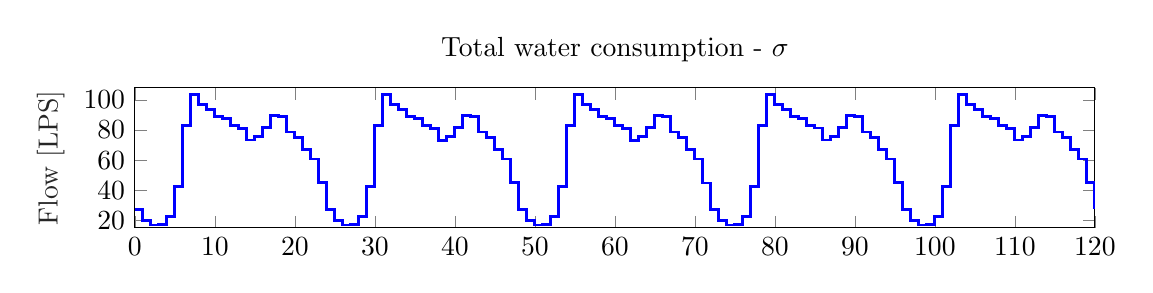
\begin{tikzpicture}

\begin{axis}[%
width=4.8in,
height=0.7in,
at={(0.888in,0.432in)},
scale only axis,
xmin=0,
xmax=120,
%xlabel style={font=\color{white!15!black}},
%xlabel={Time [h]},
ymin=15,
ymax=108,
ylabel style={font=\color{white!15!black}},
ylabel={Flow  [LPS]},
axis background/.style={fill=white},
title style={},
title={Total water consumption - $\sigma$}
]
\addplot[const plot, color=blue, line width=1pt, forget plot] table[row sep=crcr] {%
0	27.39\\
1	19.81\\
2	16.93\\
3	17.32\\
4	22.81\\
5	42.61\\
6	82.99\\
7	103.44\\
8	97.07\\
9	93.68\\
10	88.91\\
11	87.69\\
12	82.95\\
13	81.27\\
14	73.3\\
15	75.84\\
16	81.56\\
17	89.81\\
18	88.84\\
19	78.71\\
20	75.05\\
21	66.84\\
22	60.75\\
23	44.89\\
24	27.4\\
25	19.81\\
26	16.92\\
27	17.32\\
28	22.81\\
29	42.61\\
30	82.99\\
31	103.44\\
32	97.08\\
33	93.69\\
34	88.91\\
35	87.7\\
36	82.94\\
37	81.27\\
38	73.29\\
39	75.84\\
40	81.55\\
41	89.83\\
42	88.85\\
43	78.69\\
44	75.05\\
45	66.84\\
46	60.74\\
47	44.89\\
48	27.39\\
49	19.82\\
50	16.93\\
51	17.32\\
52	22.81\\
53	42.61\\
54	82.99\\
55	103.43\\
56	97.08\\
57	93.68\\
58	88.91\\
59	87.71\\
60	82.95\\
61	81.27\\
62	73.29\\
63	75.84\\
64	81.55\\
65	89.82\\
66	88.8500000000001\\
67	78.69\\
68	75.05\\
69	66.83\\
70	60.73\\
71	44.88\\
72	27.4\\
73	19.81\\
74	16.93\\
75	17.33\\
76	22.8\\
77	42.6\\
78	83\\
79	103.43\\
80	97.08\\
81	93.69\\
82	88.92\\
83	87.7\\
84	82.95\\
85	81.29\\
86	73.3\\
87	75.84\\
88	81.55\\
89	89.82\\
90	88.85\\
91	78.69\\
92	75.05\\
93	66.84\\
94	60.75\\
95	44.9\\
96	27.39\\
97	19.83\\
98	16.92\\
99	17.33\\
100	22.8\\
101	42.6\\
102	82.98\\
103	103.43\\
104	97.08\\
105	93.69\\
106	88.92\\
107	87.69\\
108	82.95\\
109	81.27\\
110	73.3\\
111	75.85\\
112	81.55\\
113	89.82\\
114	88.86\\
115	78.7\\
116	75.05\\
117	66.83\\
118	60.74\\
119	44.89\\
120	27.39\\
};
\end{axis}
\end{tikzpicture}% 
%  \vspace{-2.5mm}
%  %\caption{Consumption pattern in the identification.}
%  \label{fig:sigma_id}
%  \end{figure}
% \vspace{-8mm}

%  %Inlet flows
%  \begin{figure}[H]
%  \centering
%  %\hspace{0mm}
%  %
\includegraphics[width=0.35\textwidth]{report/pictures/missingfigure}
%  % This file was created by matlab2tikz.
%
%The latest updates can be retrieved from
%  http://www.mathworks.com/matlabcentral/fileexchange/22022-matlab2tikz-matlab2tikz
%where you can also make suggestions and rate matlab2tikz.
%
\definecolor{mycolor1}{rgb}{0.00000,0.44700,0.74100}%
\definecolor{mycolor2}{rgb}{0.85000,0.32500,0.09800}%
%
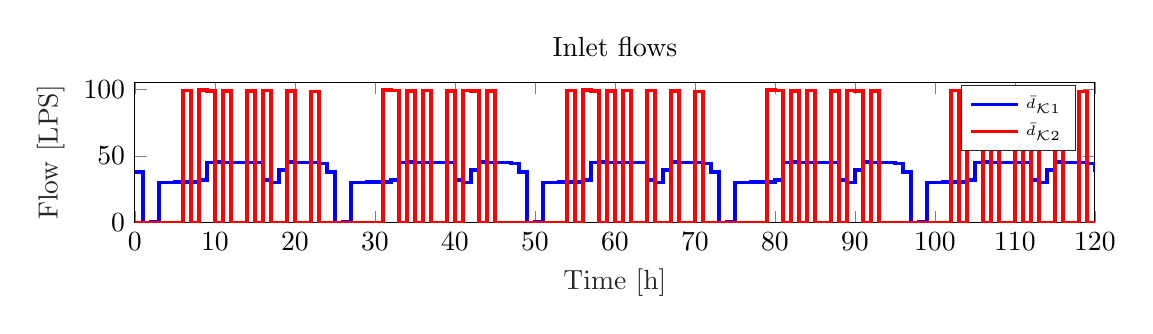
\begin{tikzpicture}

\begin{axis}[%
width=4.8in,
height=0.7in,
at={(0.758in,0.481in)},
scale only axis,
xmin=0,
xmax=120,
xlabel style={font=\color{white!15!black}},
xlabel={Time [h]},
ymin=0,
ymax=105,
ylabel style={font=\color{white!15!black}},
ylabel={Flow  [LPS]},
axis background/.style={fill=white},
title style={},
title={Inlet flows},
legend style={legend cell align=left, align=left, draw=white!15!black}
]
\addplot[const plot, color=blue, line width=1.2pt] table[row sep=crcr] {%
0	37.98\\
1	-0\\
2	0.59\\
3	30.03\\
4	30.03\\
5	30.33\\
6	30.33\\
7	30.33\\
8	31.8\\
9	45.05\\
10	45.34\\
11	45.05\\
12	44.76\\
13	45.05\\
14	44.76\\
15	45.05\\
16	31.8\\
17	30.03\\
18	39.46\\
19	45.34\\
20	45.05\\
21	44.76\\
22	45.05\\
23	44.46\\
24	37.98\\
25	-0\\
26	0.59\\
27	30.03\\
28	30.03\\
29	30.33\\
30	30.33\\
31	30.33\\
32	31.8\\
33	45.05\\
34	45.34\\
35	45.05\\
36	44.76\\
37	45.05\\
38	44.76\\
39	45.05\\
40	31.8\\
41	30.03\\
42	39.46\\
43	45.34\\
44	45.05\\
45	44.76\\
46	45.05\\
47	44.46\\
48	37.98\\
49	-0\\
50	0.59\\
51	30.03\\
52	30.03\\
53	30.33\\
54	30.33\\
55	30.33\\
56	31.8\\
57	45.05\\
58	45.34\\
59	45.05\\
60	44.76\\
61	45.05\\
62	44.76\\
63	45.05\\
64	31.8\\
65	30.03\\
66	39.46\\
67	45.34\\
68	45.05\\
69	44.76\\
70	45.05\\
71	44.46\\
72	37.98\\
73	-0\\
74	0.59\\
75	30.03\\
76	30.03\\
77	30.33\\
78	30.33\\
79	30.33\\
80	31.8\\
81	45.05\\
82	45.34\\
83	45.05\\
84	44.76\\
85	45.05\\
86	44.76\\
87	45.05\\
88	31.8\\
89	30.03\\
90	39.46\\
91	45.34\\
92	45.05\\
93	44.76\\
94	45.05\\
95	44.46\\
96	37.98\\
97	-0\\
98	0.59\\
99	30.03\\
100	30.03\\
101	30.33\\
102	30.33\\
103	30.33\\
104	31.8\\
105	45.05\\
106	45.34\\
107	45.05\\
108	44.76\\
109	45.05\\
110	44.76\\
111	45.05\\
112	31.8\\
113	30.03\\
114	39.46\\
115	45.34\\
116	45.05\\
117	44.76\\
118	45.05\\
119	44.46\\
120	37.98\\
};
\addlegendentry{\tiny $\bar{d}_{\mathcal{K}1}$}

\addplot[const plot, color=red, line width=1.2pt] table[row sep=crcr] {%
0	0\\
1	0\\
2	0\\
3	0\\
4	0\\
5	0\\
6	99.18\\
7	0\\
8	99.3\\
9	98.74\\
10	0\\
11	98.71\\
12	0\\
13	0\\
14	98.63\\
15	0\\
16	98.82\\
17	0\\
18	0\\
19	98.6\\
20	0\\
21	0\\
22	98.41\\
23	0\\
24	0\\
25	0\\
26	0\\
27	0\\
28	0\\
29	0\\
30	0\\
31	99.38\\
32	98.95\\
33	0\\
34	98.68\\
35	0\\
36	99.16\\
37	0\\
38	0\\
39	98.55\\
40	0\\
41	99.14\\
42	98.62\\
43	0\\
44	98.54\\
45	0\\
46	0\\
47	0\\
48	0\\
49	0\\
50	0\\
51	0\\
52	0\\
53	0\\
54	99.15\\
55	0\\
56	99.3\\
57	98.73\\
58	0\\
59	98.71\\
60	0\\
61	99.18\\
62	0\\
63	0\\
64	98.76\\
65	0\\
66	0\\
67	98.58\\
68	0\\
69	0\\
70	98.4\\
71	0\\
72	0\\
73	0\\
74	0\\
75	0\\
76	0\\
77	0\\
78	0\\
79	99.38\\
80	98.94\\
81	0\\
82	98.68\\
83	0\\
84	99.15\\
85	0\\
86	0\\
87	98.54\\
88	0\\
89	99.15\\
90	98.62\\
91	0\\
92	98.55\\
93	0\\
94	0\\
95	0\\
96	0\\
97	0\\
98	0\\
99	0\\
100	0\\
101	0\\
102	99.17\\
103	0\\
104	99.3\\
105	98.74\\
106	0\\
107	98.71\\
108	0\\
109	0\\
110	98.64\\
111	0\\
112	98.76\\
113	0\\
114	0\\
115	98.59\\
116	0\\
117	0\\
118	98.4\\
119	0\\
120	0\\
};
\addlegendentry{\tiny $\bar{d}_{\mathcal{K}2}$}

\end{axis}
\end{tikzpicture}% 
%  \vspace{-2.5mm}
%  \caption{Inlet flows of the two pumping stations.}
%  \label{fig:dk_12}
%  \end{figure}
%  \vspace{-3mm}